% document class -------------------------------------------
\documentclass[11pt,oneside,openright]{./style/phdthesis}
% ----------------------------------------------------------

% my definitions -------------------------------------------
%\def\bob()
%\def\dynamicHED{}
%\def\estimatorEntropy
%\def\qpsk{}
%\def\optical{}
%\def\bpsk{}
%\def\hammingED{}
%\def\huffmanED{}
%\def\arithemeticED{}
%\def\miEstimator{}
\def\mQAM{}
%\def\lBmQAM{}
%%\def\sdf{}
%\def\rofKK{}
%\def\dsp{}
%\def\quantumRNG{}
%\def\bb{}
%\def\qokd{}
%\def\dv{}
%\def\quantumA{}
%\def\cvQuantum{}
%\def\qkdCvWithoutBS{}
%\def\intradyne{}
%\def\classicalMpc{}
%\def\quantumMpc{}
%\def\secureMPC{}
%\def\tinyGarble{}
%

% ----------------------------------------------------------

% my packages ----------------------------------------------
\usepackage{amsmath}


\usepackage[ansinew]{inputenc}
%\usepackage[portuguese]{babel}
\usepackage[printonlyused, withpage]{acronym}
\usepackage{a4wide}
\usepackage{palatino}
\usepackage{fancyhdr}
\usepackage{fancybox}
\usepackage{amssymb}

% biblatex ------------------------------------------------------------------------------------------
% used to divide the bibliography into multiple parts for example per chapter or per section
\usepackage[sorting=none, backend=biber]{biblatex}
% ---------------------------------------------------------------------------------------------------

%\usepackage{chapterbib} %com este package as referencias bibliográficas aparecem no final de cada capítulo
%\usepackage{cite}
\usepackage{epsfig}
%\usepackage{subfigure}
\usepackage{graphics}
\usepackage{float}                   % figures place here [H]
\usepackage{here}
\usepackage[T1]{fontenc}
\usepackage{rotating}
\usepackage{multirow}
%\usepackage{comment}
%\usepackage{captionhack}
\usepackage{epigraph}
\usepackage[linkcolor=black]{hyperref}
%\renewcommand{\thesubfigure}{}
\hypersetup{colorlinks=true}
\usepackage{enumerate}
%\usepackage[numbers,sort&compress]{natbib}
%\usepackage{hypernat}
\usepackage{booktabs}
\usepackage{url}                    % needed to cite a site
\usepackage{eurosym}
\usepackage{makeidx}
\usepackage{datatool}
\usepackage[toc, acronym]{glossaries}

% graphicx -----------------------------------------------------------------------------------
% The graphicx package allows to specify several paths in which to search for figures.
\usepackage{graphicx}
% --------------------------------------------------------------------------------------------

\usepackage{caption}
\usepackage{subcaption}

\usepackage{longtable}				% Multi-page tables
\usepackage{tabulary}
\usepackage{braket}

% subfile handling packages
\usepackage{subfiles}

% For box
\usepackage{multicol}
\usepackage{tcolorbox}
\usepackage{booktabs}

% For flow chart
\usepackage{tikz}
\usetikzlibrary{shapes,arrows}

\usepackage{epstopdf}
\usepackage{listings}
\usepackage{color}
\usepackage{textcomp,xcolor}

\usepackage{mathrsfs}


% amsfonts ------------------------------------------------------------------------------------------
% Provides symbols for the number sets (prime, natural, integer, rational, real and complex) in LaTeX
\usepackage{amsfonts}
% ---------------------------------------------------------------------------------------------------

% ----------------------------------------------------------

% my bib files ---------------------------------------------
%%%%%%%%%%%%%%%%%%%%%%%%%%%%%%%%%%%%%%%%%%%%%%%%%%%%%%%%%%%%%%%%%%%%%%%%%%%%%%%%%%
% Bibliography for the Simulator Strucuture
%%%%%%%%%%%%%%%%%%%%%%%%%%%%%%%%%%%%%%%%%%%%%%%%%%%%%%%%%%%%%%%%%%%%%%%%%%%%%%%%%%

\addbibresource{./chapter/simulator_structure/simulator_structure.bib}

%%%%%%%%%%%%%%%%%%%%%%%%%%%%%%%%%%%%%%%%%%%%%%%%%%%%%%%%%%%%%%%%%%%%%%%%%%%%%%%%%%
% Bibliography for SDF
%%%%%%%%%%%%%%%%%%%%%%%%%%%%%%%%%%%%%%%%%%%%%%%%%%%%%%%%%%%%%%%%%%%%%%%%%%%%%%%%%%

\ifdefined\qpsk                 \addbibresource{./sdf/qpsk_transmitter/qpsk_transmitter.bib}\fi
\ifdefined\optical              \addbibresource{./sdf/optical_detection/optical_detection.bib}\fi
\ifdefined\bpsk                 \addbibresource{./sdf/bpsk_system/bpsk_system.bib}\fi
\ifdefined\mQAM                 \addbibresource{./sdf/m_qam_system/m_qam_system.bib}\fi
\ifdefined\hammingED            \addbibresource{./sdf/eit_25828_hamming_channel_encoder_decoder/eit_25828_hamming_channel_encoder_decoder.bib}\fi
\ifdefined\huffmanED            \addbibresource{./sdf/eit_45550_estimator_source_code_efficiency/eit_45550_estimator_source_code_efficiency.bib}\fi
\ifdefined\arithmeticED         \addbibresource{./sdf/eit_46084_arithmetic_encoder_decoder/eit_46084_arithmetic_encoder_decoder.bib}\fi
\ifdefined\miEstimator          \addbibresource{./sdf/eit_87071_mutual_information_estimator/eit_87071_mutual_information_estimator.bib}\fi
\ifdefined\dynamicHED           \addbibresource{./sdf/eit_64926_dynamic_huffman_encoder_decoder/eit_64926_dynamic_huffman_encoder_decoder.bib}\fi
\ifdefined\estimatorEntropy     \addbibresource{./sdf/eit_42256_estimator_entropy/eit_42256_estimator_entropy.bib}\fi
\ifdefined\lBmQAM               \addbibresource{./sdf/low_baud_m_qam_system/low_baud_m_qam_system.bib}\fi
\ifdefined\simplified           \addbibresource{./sdf/simplified_coherent_receiver/simplified_coherent_receiver.bib}\fi
\ifdefined\rofKK	            \addbibresource{./sdf/kramers_kronig_transceiver/kramers_kronig_transceiver.bib}\fi
\ifdefined\dsp                  \addbibresource{./sdf/dsp_laser_phase_compensation/dsp_laser_phase_compensation.bib}\fi
\ifdefined\quantumRNG           \addbibresource{./sdf/quantum_random_number_generator/quantum_random_number_generator.bib}\fi
\ifdefined\bb                   \addbibresource{./sdf/bb84_with_discrete_variables/bb84_with_discrete_variables.bib}\fi
\ifdefined\qokd                 \addbibresource{./sdf/qokd_with_discrete_variables/qokd_with_discrete_variables.bib}\fi
\ifdefined\dv                   \addbibresource{./sdf/dv_polarization_encoding_system/dv_polarization_encoding_system.bib}\fi
\ifdefined\bob                  \addbibresource{./sdf/dv_polarization_encoding_system_bob_processor/dv_polarization_encoding_system_bob_processor.bib}\fi
\ifdefined\quantumA             \addbibresource{./sdf/quantum_noise/quantum_noise.bib}\fi
\ifdefined\cvQuantum            \addbibresource{./sdf/cv_system/cv_system.bib}\fi
\ifdefined\intradyne            \addbibresource{./sdf/intradyne_cv_system/intradyne_cv_system.bib}\fi
\ifdefined\classicalMpc         \addbibresource{./sdf/classical_mpc/classical_mpc.bib}\fi
\ifdefined\quantumMpc           \addbibresource{./sdf/quantum_mpc/quantum_mpc.bib}\fi
\ifdefined\secureMPC            \addbibresource{./sdf/secure_multiparty_computation/secure_multiparty_computation.bib}\fi
\ifdefined\qkdCvWithoutBS       \addbibresource{./sdf/qkd_with_cv_without_base_switching/qkd_with_cv_without_base_switching.bib}\fi



%%%%%%%%%%%%%%%%%%%%%%%%%%%%%%%%%%%%%%%%%%%%%%%%%%%%%%%%%%%%%%%%%%%%%%%%%%%%%%%%%%
% Bibliography for the Library
%%%%%%%%%%%%%%%%%%%%%%%%%%%%%%%%%%%%%%%%%%%%%%%%%%%%%%%%%%%%%%%%%%%%%%%%%%%%%%%%%%

\addbibresource{./lib/bit_error_rate/bit_error_rate.bib}
\addbibresource{./lib/iir_filter/iir_filter.bib}
\addbibresource{./lib/iq_modulator/iq_modulator.bib}

%%%%%%%%%%%%%%%%%%%%%%%%%%%%%%%%%%%%%%%%%%%%%%%%%%%%%%%%%%%%%%%%%%%%%%%%%%%%%%%%%%
% Bibliography for the Algorithms
%%%%%%%%%%%%%%%%%%%%%%%%%%%%%%%%%%%%%%%%%%%%%%%%%%%%%%%%%%%%%%%%%%%%%%%%%%%%%%%%%%

\addbibresource{./algorithms/fft/fft.bib}
\addbibresource{./algorithms/overlap_save/overlap_save.bib}
\addbibresource{./algorithms/filter/filter.bib}
\addbibresource{./algorithms/hilbert/hilbert.bib}

%%%%%%%%%%%%%%%%%%%%%%%%%%%%%%%%%%%%%%%%%%%%%%%%%%%%%%%%%%%%%%%%%%%%%%%%%%%%%%%%%%
% Bibliography for the GitHelper
%%%%%%%%%%%%%%%%%%%%%%%%%%%%%%%%%%%%%%%%%%%%%%%%%%%%%%%%%%%%%%%%%%%%%%%%%%%%%%%%%%

\addbibresource{./chapter/git/git_helper.bib} 
%----------------------------------------------------------

% my commands ----------------------------------------------
\newcommand{\onlyinsubfile}[1]{#1}
\newcommand{\notinsubfile}[1]{}
\renewcommand{\textfraction}{0.01}
\renewcommand{\topfraction}{0.99}
\renewcommand{\floatpagefraction}{0.99}
\renewcommand{\bottomfraction}{0.99}
\renewcommand{\heavyrulewidth}{1pt}
\renewcommand{\lightrulewidth}{0.50pt}
\renewcommand{\chaptername}{Chapter}
\renewcommand{\figurename}{Figure}
\renewcommand{\appendixname}{\Large{Anex}}
\renewcommand{\tablename}{Table}
\renewcommand{\acronymname}{Acronimous}

\newcommand{\mli}[1]{\mathit{#1}}
\newcommand{\intSpace}{\!\!\!\!}
\newcommand{\doubleInt}{\!\!\int\intSpace\int\!\!}
\newcommand{\TX}{\mathit{TX}}
\newcommand{\NLI}{\mathit{NLI}}
\newcommand{\eff}{\mathit{eff}}
\newcommand{\LOASE}{\mathit{LO-ASE}}
\newcommand{\LONLI}{\mathit{LO-NLI}}


%\makesavenoteenv{tabular}



\hyphenpenalty=50000
\tolerance=10000
%%% General page formatting

\oddsidemargin 0.2in
\evensidemargin 0in
%\textwidth 155mm
\headheight 15.0pt
\topmargin 0in
%\textheight 237mm

% footheight 1.0in

\makeatletter
\providecommand*{\diff}%
{\@ifnextchar^{\DIfF}{\DIfF^{}}}
\def\DIfF^#1{%
\mathop{\mathrm{\mathstrut d}}%
\nolimits^{#1}\gobblespace}
\def\gobblespace{%
\futurelet\diffarg\opspace}
\def\opspace{%
\let\DiffSpace\!%
\ifx\diffarg(%
\let\DiffSpace\relax
\else
\ifx\diffarg[%
\let\DiffSpace\relax
\else
\ifx\diffarg\{%
\let\DiffSpace\relax
\fi\fi\fi\DiffSpace}

\providecommand*{\tDeriv}[3][]{%
\frac{\diff^{#1}#2}{\diff #3^{#1}}}
\providecommand*{\pDeriv}[3][]{%
\frac{\partial^{#1}#2}%
{\partial #3^{#1}}}



\DeclareMathOperator{\erf}{erf}
\DeclareMathOperator{\erfc}{erfc}
\DeclareMathOperator{\sinc}{sinc}
\DeclareMathOperator{\R}{Re}
\DeclareMathOperator{\I}{Im}
\DeclareMathOperator{\asinh}{asinh}

%\newcommand{\publ}{}

\pagenumbering{arabic} 
% ----------------------------------------------------------

% my figures ----------------------------------------------
\graphicspath{
    {./figures/}
    {./sdf/bpsk_system/figures/}
    {./sdf/cv_system/figures/}
    {./chapter/git/figures/}
    }
% ----------------------------------------------------------

% index ----------------------------------------------------
\makeindex
% ----------------------------------------------------------

\begin{document}

% title -----------------------------------------------------
\title{NetXPTO - LinkPlanner}
\author{Armando Nolasco Pinto}
\date{\today}
\maketitle
% -----------------------------------------------------------

% table of contents -----------------------------------------
\tableofcontents
% -----------------------------------------------------------

% chapters --------------------------------------------------

% ------------------------------------------------------------------------
\chapter{Preface}






% ------------------------------------------------------------------------
\chapter{Introduction}

LinkPlanner is devoted to the simulation of point-to-point links.







% ------------------------------------------------------------------------
\chapter{Simulator Structure}

LinkPlanner is a signals open-source simulator.

The major entity is the system.

A system comprises a set of blocks.

The blocks interact with each other through signals.

\section{System}

\section{Blocks}

\section{Signals}

List of available signals:

\begin{itemize}
    \item Signal

\end{itemize}










% ------------------------------------------------------------------------
\chapter{Development Cycle}

The NetXPTO-LinkPlanner is a open source project with its core implemented using ISO C++.
At the present the followed standard is the ISO C++14.


The developed environment has been the Visual Studio Community 2017, namely release 15.5 and beyond.
The Git has been used as the version control system.
The NetXPTO-LinkPlanner repository is located in the GitHub site http://github.com/netxpto/linkplanner.
Master branch should be considered a functional beta version of the software.
Periodically new releases are delivered from the master branch under the branch name R<Release Year>-<Release Number>.
The design and integration of the system has been performed by Prof. Armando Pinto.





\include{chapter/visualizer}

% ------------------------------------------------------------------------
\chapter{Case Studies}

\ifdefined\qpsk         	\section{QPSK Transmitter}

This system simulates a QPSK transmitter. A schematic representation of this system is shown in figure \ref{QPSK_transmitter_block_diagram_simple}.

\begin{figure}[h]
	\centering
	\includegraphics[width=0.5\textwidth]{figures/qpsk_transmitter.pdf}
	\caption{QPSK transmitter block diagram}\label{QPSK_transmitter_block_diagram_simple}
\end{figure}

\subsection*{Functional description}

This block generates an optical signal (output signal 1 in figure \ref{MQAM_transmitter_block_diagram}). The binary signal generated in the internal block Binary Source (block B1 in figure \ref{MQAM_transmitter_block_diagram}) can be used to perform a Bit Error Rate (BER) measurement and in that sense it works as an extra output signal (output signal 2 in figure \ref{MQAM_transmitter_block_diagram}).

\begin{figure}[h]
	\centering
	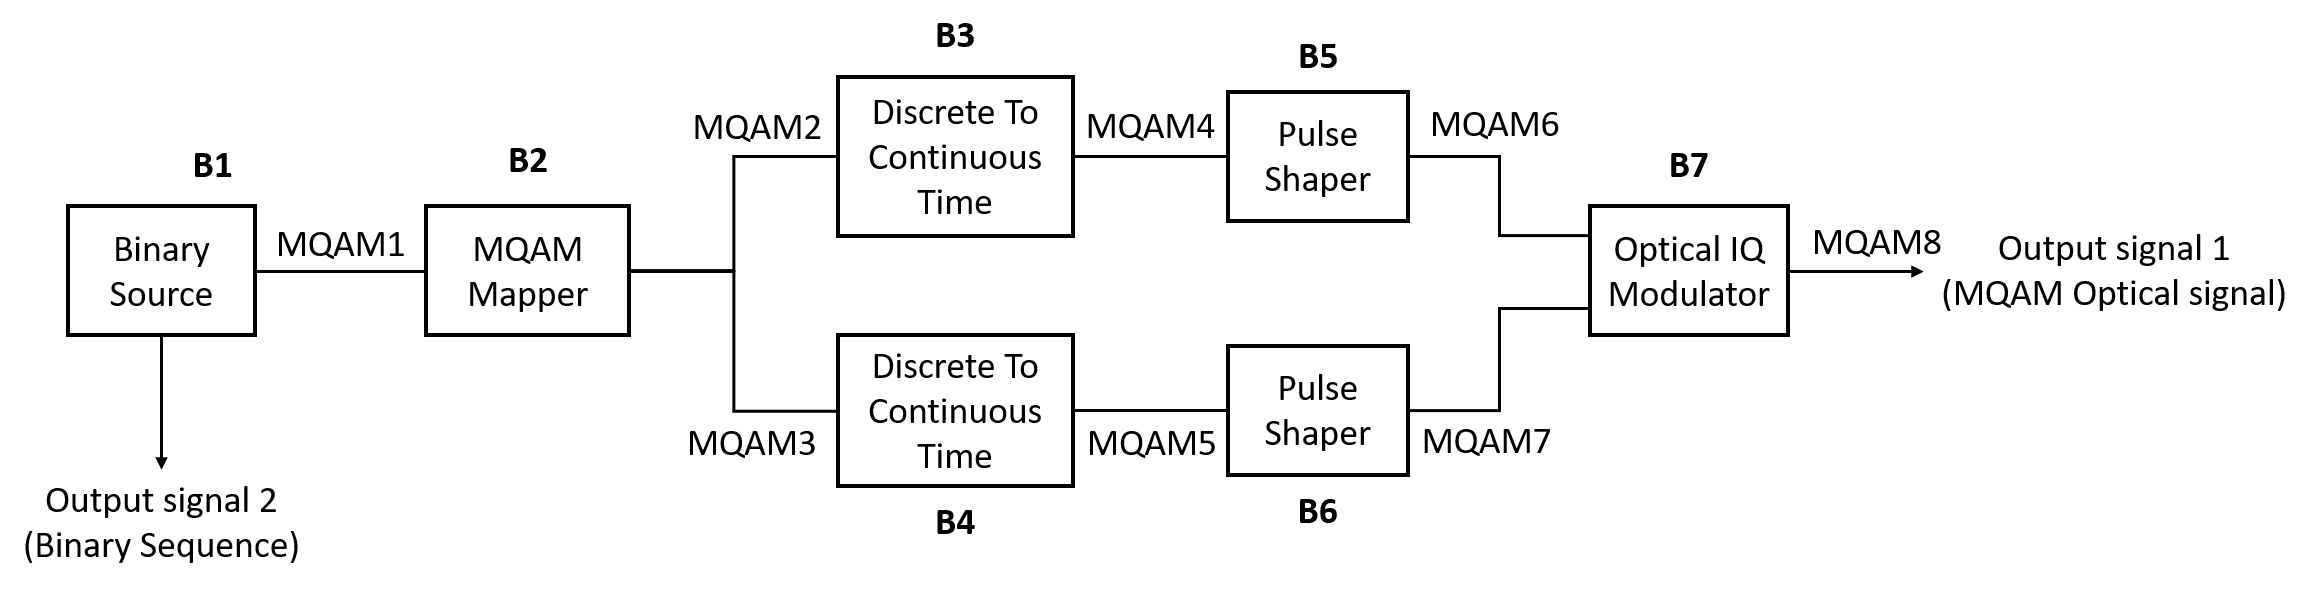
\includegraphics[width=\textwidth]{figures/MQAM_transmitter_block_diagram}
	\caption{Schematic representation of the block MQAM transmitter.}\label{MQAM_transmitter_block_diagram}
\end{figure}

\subsection*{Input parameters}

This block has a special set of functions that allow the user to change the basic configuration of the transmitter. The list of input parameters, functions used to change them and the values that each one can take are summarized in table \ref{table}.

\begin{table}[h]
\begin{center}
	\begin{tabular}{| m{3,5cm} | m{5,1cm} |  m{2,5cm} | m{4cm} | }
		\hline
		\textbf{Input parameters} & \textbf{Function} & Type & \textbf{Accepted values} \\ \hline
		Mode & setMode() & string & PseudoRandom \newline Random \newline DeterministicAppendZeros \newline DeterministicCyclic \\ \hline
		Number of bits generated & setNumberOfBits() & int & Any integer\\ \hline
		Pattern length & setPatternLength() & int & Real number greater than zero\\ \hline
		Number of bits & setNumberOfBits() & long & Integer number greater than zero\\ \hline
		Number of samples per symbol & setNumberOfSamplesPerSymbol() & int & Integer number of the type $2^n$ with n also integer\\ \hline
		Roll of factor & setRollOfFactor() & double & $\in$ [0,1] \\ \hline
		IQ amplitudes & setIqAmplitudes() & Vector of coordinate points in the I-Q plane & \textbf{Example} for a 4-qam mapping: \{ \{ 1.0, 1.0 \}, \{ -1.0, 1.0 \}, \{ -1.0, -1.0 \}, \{ 1.0, -1.0 \} \} \\ \hline
		Output optical power & setOutputOpticalPower() & int & Real number greater than zero\\ \hline
		Save internal signals & setSaveInternalSignals() & bool & True or False\\
		\hline
	\end{tabular}
	\caption{List of input parameters of the block MQAM transmitter} \label{table}
\end{center}
\end{table}

%\begin{itemize}
%	\item setMode(PseudoRandom);
%	\item setBitPeriod(1.0/50e9);
%	\linebreak (double)
%	\item setPatternLength(3);
%	\linebreak (int)
%	\item setNumberOfBits(10000);
%	\linebreak (long)
%	\item setNumberOfSamplesPerSymbol(32);
%	\linebreak (int)
%	\item setRollOffFactor(0.9);
%	\linebreak (double $\in$ [0,1])
%	\item setIqAmplitudes(\{ \{ 1, 1 \}, \{ -1, 1 \}, \{ -1, -1 \}, \{ 1, -1 \} \});
%	\item setOutputOpticalPower\_dBm(0);
%	\item setSaveInternalSignals(true);
%\end{itemize}

\pagebreak

\subsection*{Methods}

MQamTransmitter(vector$<$Signal *$>$ \&inputSignal, vector$<$Signal *$>$ \&outputSignal); (\textbf{constructor})
\bigbreak

void set(int opt);
\bigbreak
void setMode(BinarySourceMode m)
\bigbreak
BinarySourceMode const getMode(void)
\bigbreak
void setProbabilityOfZero(double pZero)
\bigbreak
double const getProbabilityOfZero(void)
\bigbreak
void setBitStream(string bStream)
\bigbreak
string const getBitStream(void)
\bigbreak
void setNumberOfBits(long int nOfBits)
\bigbreak
long int const getNumberOfBits(void)
\bigbreak
void setPatternLength(int pLength)
\bigbreak
int const getPatternLength(void)
\bigbreak
void setBitPeriod(double bPeriod)
\bigbreak
double const getBitPeriod(void)
\bigbreak
void setM(int mValue)
int const getM(void)
\bigbreak
void setIqAmplitudes(vector$<$t\textunderscore iqValues$>$ iqAmplitudesValues)
\bigbreak
vector$<$t\textunderscore iqValues$>$ const getIqAmplitudes(void)
\bigbreak
void setNumberOfSamplesPerSymbol(int n)
\bigbreak
int const getNumberOfSamplesPerSymbol(void)
\bigbreak
void setRollOffFactor(double rOffFactor)
\bigbreak
double const getRollOffFactor(void)
\bigbreak
void setSeeBeginningOfImpulseResponse(bool sBeginningOfImpulseResponse)
\bigbreak
double const getSeeBeginningOfImpulseResponse(void)
\bigbreak
void setOutputOpticalPower(t\textunderscore real outOpticalPower)
\bigbreak
t\textunderscore real const getOutputOpticalPower(void)
\bigbreak
void setOutputOpticalPower\_dBm(t\_real outOpticalPower\_dBm)
\bigbreak
t\_real const getOutputOpticalPower\_dBm(void)
\pagebreak

\subsection*{Output Signals}

\subparagraph*{Number:} 1 optical and 1 binary (optional)

\subparagraph*{Type:} Optical signal

\subsection*{Example}

\begin{figure}[h]
	\centering
	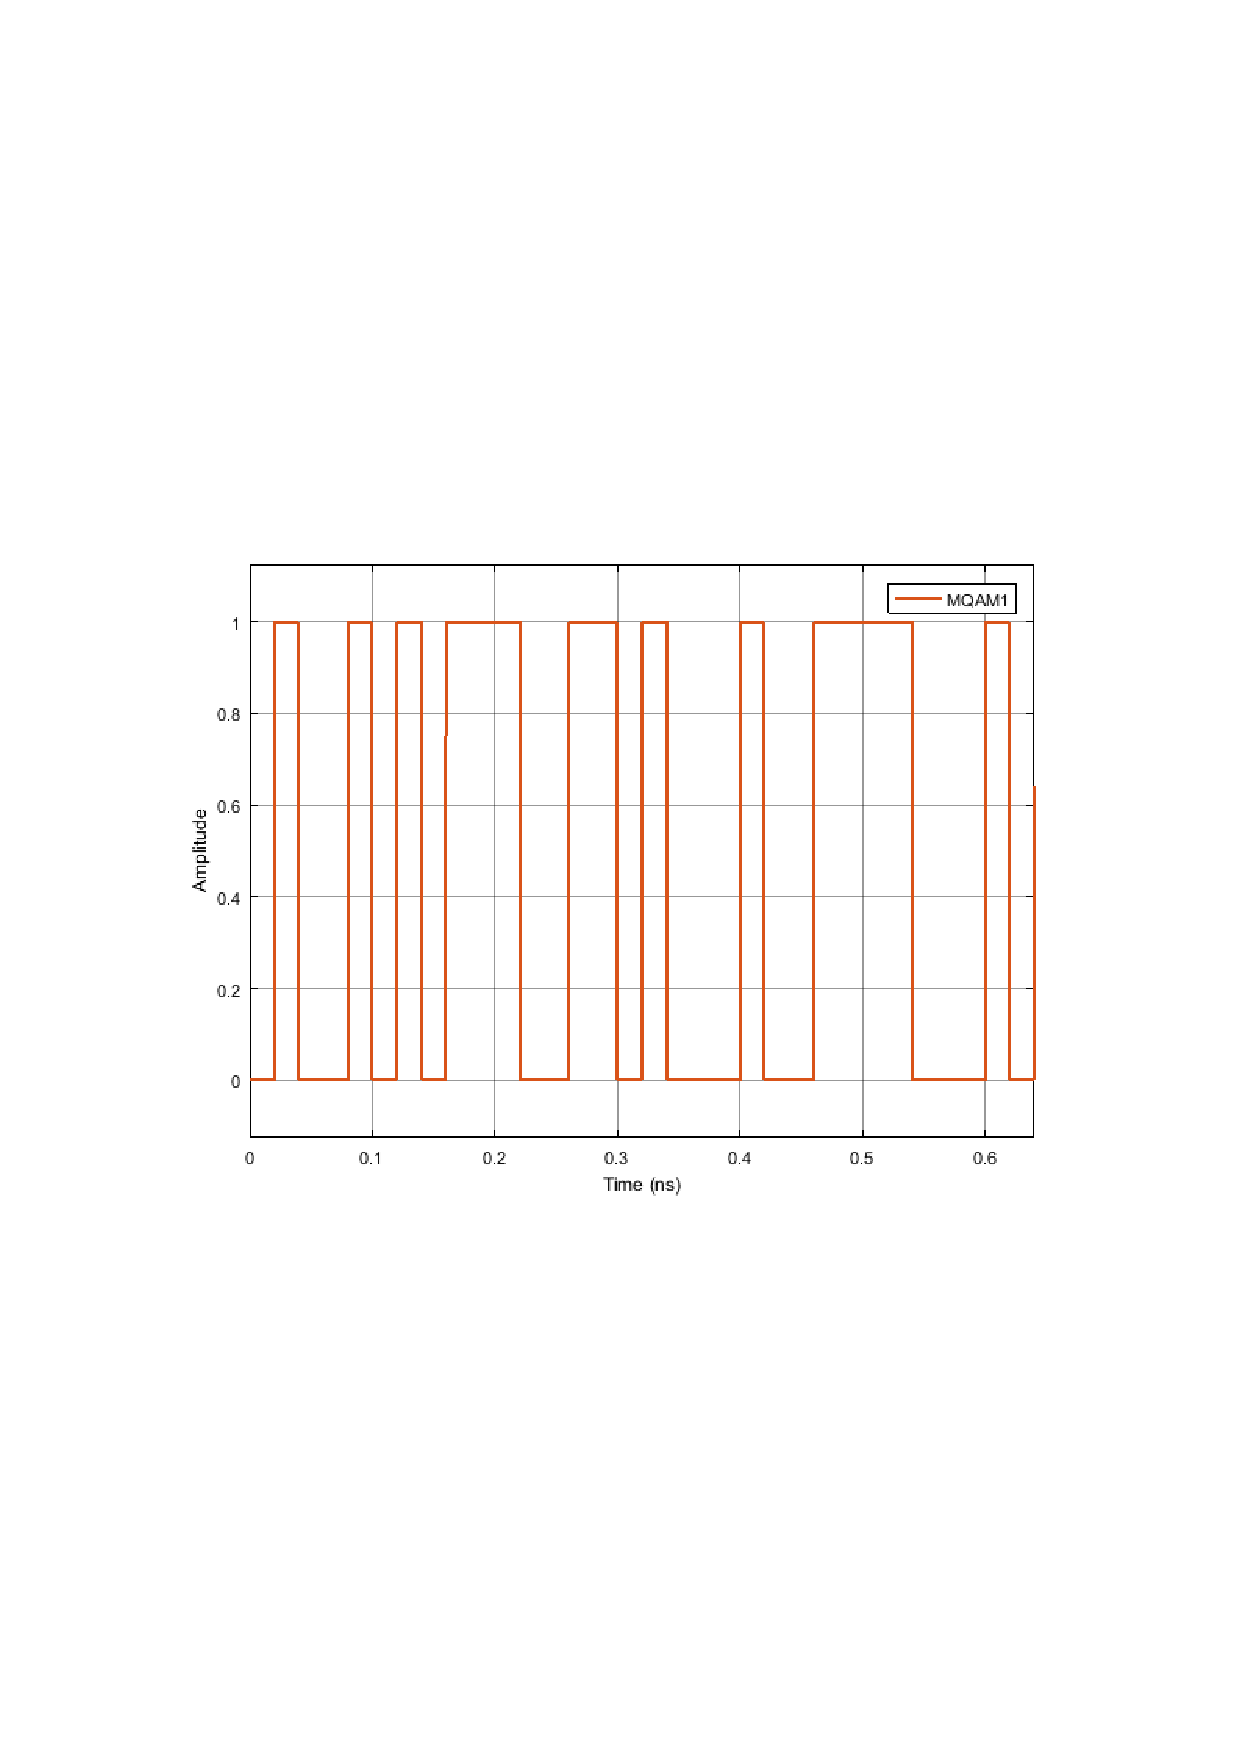
\includegraphics[width=0.8\textwidth]{figures/BinarySource_output}
	\caption{Example of the binary sequence generated by this block for a sequence 0100...}
\end{figure}

\begin{figure}[h]
	\centering
	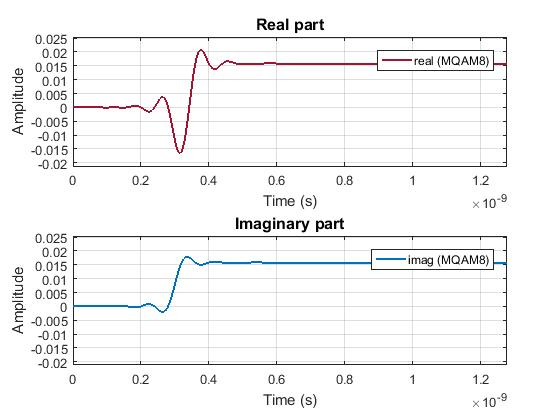
\includegraphics[width=0.8\textwidth]{figures/IQmodulator0_output}
	\caption{Example of the output optical signal generated by this block for a sequence 0100...}
\end{figure}

\subsection*{Sugestions for future improvement}

Add to the system another block similar to this one in order to generate two optical signals with perpendicular polarizations. This would allow to combine the two optical signals and generate an optical signal with any type of polarization.
 \fi
\ifdefined\optical      	\input{./sdf/optical_detection/optical_detection} \fi
\ifdefined\bpsk         	\input{./sdf/bpsk_system/bpsk_system} \fi
\ifdefined\hammingED        \input{./sdf/eit_25828_hamming_channel_encoder_decoder/eit_25828_hamming_channel_encoder_decoder}\fi
\ifdefined\huffmanED        \input{./sdf/eit_45550_estimator_source_code_efficiency/eit_45550_estimator_source_code_efficiency}\fi
\ifdefined\arithemeticED    \input{./sdf/eit_46084_arithmetic_encoder_decoder/eit_46084_arithmetic_encoder_decoder}\fi
\ifdefined\miEstimator      \input{./sdf/eit_87071_mutual_information_estimator/eit_87071_mutual_information_estimator}\fi
\ifdefined\dynamicHED       \input{./sdf/eit_64926_dynamic_huffman_encoder_decoder/eit_64926_dynamic_huffman_encoder_decoder}\fi
\ifdefined\estimatorEntropy \input{./sdf/eit_42256_estimator_entropy/eit_42256_estimator_entropy}\fi
\ifdefined\mQAM         	%! TEX root = ../../main_netxpto.tex
\clearpage



\section{M-QAM Transmission System}


% Show subsubsections on the Table of Contents
\setcounter{tocdepth}{3}
\setcounter{secnumdepth}{3}

\begin{refsection}
	\begin{tcolorbox}
		\begin{tabular}{p{2.75cm} p{0.2cm} p{10.5cm}}
			\textbf{Student Name} & & Andoni Santos (2018/01/03 - )\\
														& & Ana Luisa Carvalho (2017/04/01 - 2017/12/31) \\
			\textbf{Goal}         &:& M-QAM system implementation with BER measurement and comparison with theoretical and experimental values.\\
			\textbf{Directory} &:& sdf/m\_qam\_system
		\end{tabular}
	\end{tcolorbox}

	\subsection{Introduction}

	The goal of this project is to simulate a Quadrature Amplitude Modulation
	transmission system with M points in the constellation diagram (M-QAM) and to
	perform a Bit Error Rate (BER) measurement that can be compared with theoretical
	and experimental values.
	M-QAM systems can encode $\log_2 M$ bits per symbol which means they can
	transmit higher data rates keeping the same bandwidth. However, because the states are closer together, these
	systems require a higher signal-to-noise ratio.
	The Bit Error Rate (BER) is a measurement of how a bit stream is altered by a
	transmission system due to noise or intersymbol interference.

	For $M=4$ the M-QAM system can be reduced to a Quadrature Phase Shift Keying
	system (QPSK) system that uses four equispaced points in the constellation
	diagram, as shown in figure \ref{fig:const_2m} where a Gray encoding is
	assumed~\cite{proakis08}.

	\begin{figure}[H]
		\centering
		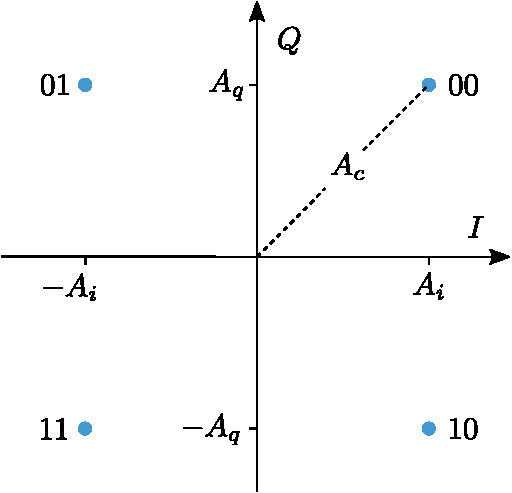
\includegraphics[width=0.5\textwidth]{./sdf/m_qam_system/figures/intro/constellation.pdf}
		\caption{A QPSK constellation, assuming $ A = A_i = A_q =
			A_c/\sqrt{2}$.\label{fig:const_2m}}
	\end{figure}

    %! TEX root = ../../main_netxpto.tex
	\subsection{Theoretical Analysis}\label{sec:mqamTeor}
	\subsubsection{QPSK Transmitter}
	\begin{figure}[H]
		\centering
		\centering
		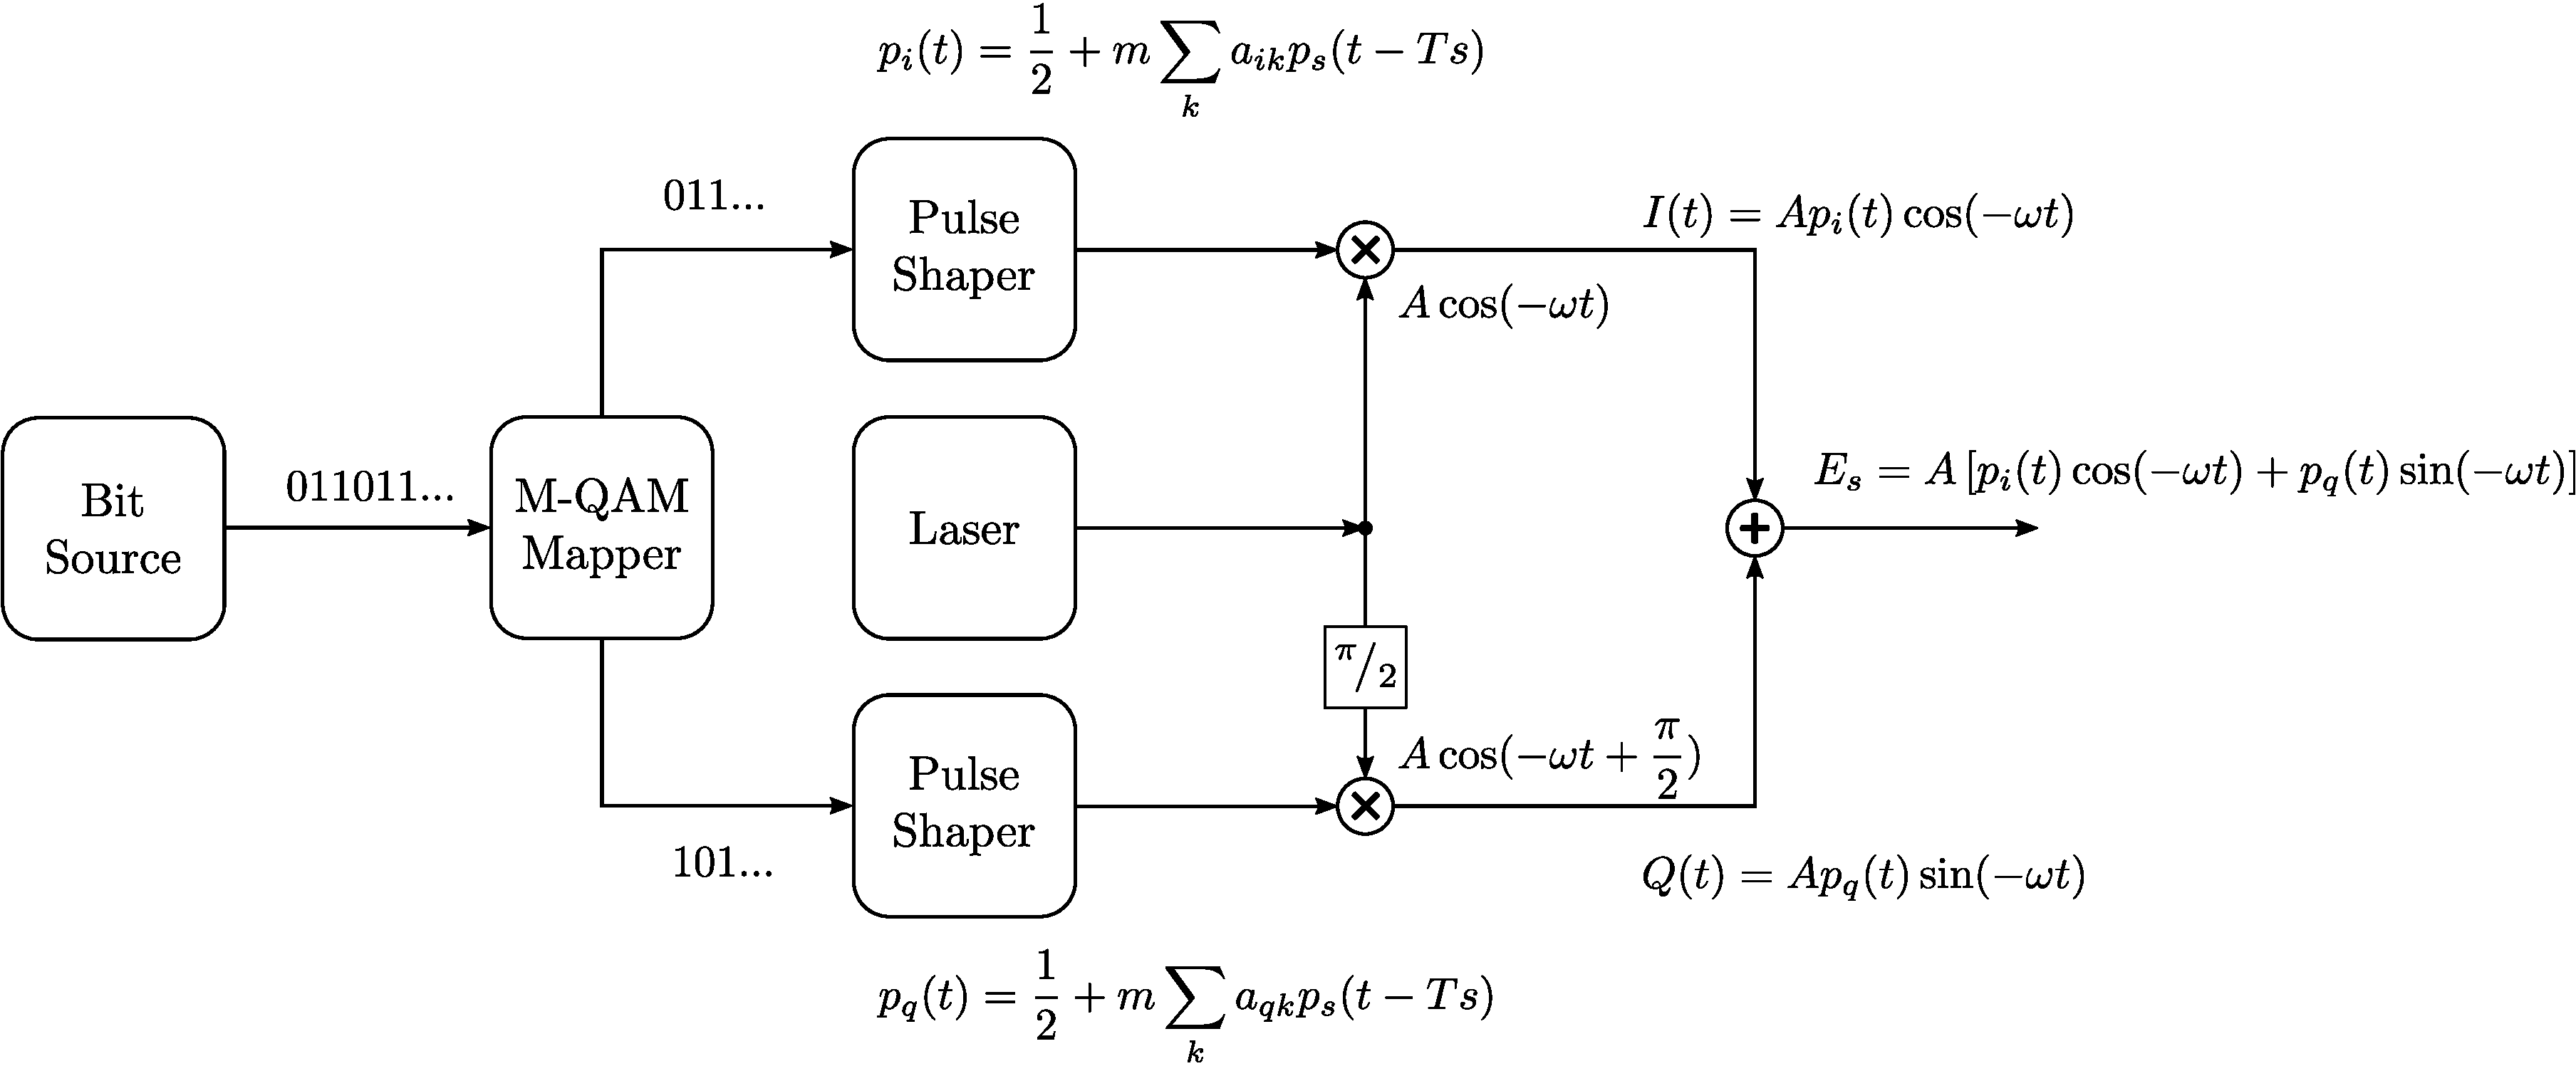
\includegraphics[
		width=0.95\textwidth]{./sdf/m_qam_system/figures/txDiagramTeor.pdf}
		\caption{Transmitter diagram.}
		\label{fig:txDiagramTeor}
	\end{figure}

	M-QAM is a modulation scheme that takes advantage of two sinusoidal carriers
	with a phase difference of $\pi/2$. The resultant output consists of a signal
	with both amplitude and phase variations. For the particular case of M = 4, it
	can be considered that $A_i = A_q = A$ , and therefore $A_c = A \sqrt{2}$.
	The two carriers, referred to as I (In-phase) and Q (Quadrature), can be
	represented as~\cite{carlson86}:

	\begin{align}\label{eq:pulsesi}
		I(t) &= p_i(t) A \cos(-\omega t) \\
		Q(t) &= p_q(t) A \cos\left(-\omega t + \frac{\pi}{2}\right) = p_q(t) A \sin(-\omega
		t) \label{eq:pulsesq}
	\end{align}

	Here, $p_i(t)$ and $p_q(t)$ is the sequence of pulses for each of the
	components, as defined by:

	\begin{equation}\label{eq:pulseDef}
				p(t) = \frac{1}{2}+m \sum_k{a_k p_s(t-T_s)},
				\qquad a_k =
					\begin{cases}
						-1       & \text{if bit} = 1, \\
						1        & \text{if bit} = 0
					\end{cases}
	\end{equation}

	\noindent where m is a scaling coefficient, to ensure the following
	conditions are met

	\begin{equation*}
		\begin{cases}
			\frac{1}{2}+m \left(\max\left\{p_s(t)\right\}\right) = 1 \\
			\frac{1}{2}+m p_s(t) > 0
		\end{cases}
	\end{equation*}

	Following from equations~\ref{eq:pulsesi} and~\ref{eq:pulsesq}, we
	have~\cite{apostol67,oo12}:

	\begin{equation}\label{eq:sigEq}
		\begin{split}
			E_s(t) &= I(t) + Q(t)  = \\
					 &= p_i(t) A\cos(-\omega t)+ p_q(t) A\sin(-\omega t) \\
					 &= p_i(t) A\cos(\omega t)- p_q(t) A\sin(\omega t) \\
					 &= A \sqrt{p_i^2(t) + p_q^2(t)} \cos{\left(- \omega t +
					 \phi_s(t)\right)}, \quad  \phi_s(t)=
					 \operatorname{arctan}{\left({p_q(t)},{p_i(t)}\right)}
		\end{split}
	\end{equation}

	The \textit{arctan} function shown above is the two argument arctangent
	function, sometimes also called \textit{atan2}. While
	the normal arctangent is defined only for the interval~$\left]-\frac{\pi}{2},
	+\frac{\pi}{2}\right]$, the two argument arctangent is a piecewise function
defined in the interval~$\left]-{\pi}, +{\pi}\right]$~\cite{glisson11}.

	\begin{align}
		\arctan(x,y) = \begin{cases}
			\arctan(y/x),                                  & if x > 0,\\
			\left(\operatorname{sign}\left\{y\right\}\right) \left({\pi}/{2}\right)  & if x = 0~\text{and}~y \neq 0, \\
			\pi +  \operatorname{arctan}({y/x})            & if x < 0, \\
			0,                                             & if x = 0~\text{and}~y = 0
		\end{cases}
	\end{align}

%		a(t) = \begin{cases}
%			A               & 0 \le t \le T_s\\
%			0               & t > T_s\\
%		\end{cases}

%	The expression for the electric field when $t_s = n T_s$ becomes:
%
%	\begin{equation}\label{eq:elFieldConst}
%		\begin{split}
%			E_s(t) &= {A} \sqrt{2} \cos{\left[ -\omega t
%					 +\operatorname{arctan}{(p_q(t_s), p_i(t_s))} \right]}\\
%					 &= \frac{A_c}{\sqrt{2}} \sqrt{2} \cos{\left[ -\omega t
%					 +\operatorname{arctan}{(p_q(t_s), p_i(t_s))} \right]}\\
%					 &= A_c \cos{\left( -\omega t + \phi_s(t)\right)}
%%						 \quad \phi_s(t)\in \left[\frac{\pi}{4},\frac{3\pi}{4},\frac{5\pi}{4},\frac{7\pi}{4} \right]
%		\end{split}
%	\end{equation}


	\subsubsection{QPSK Receiver}\label{sec:teorRX}
	We will consider a homodyne receiver with phase diversity. This is a
	configuration which uses a local oscillator with the same optical frequency,
	and measures both the in-phase and the quadrature component at the same time.

	A typical configuration for this receiver is shown in
	Figure~\ref{fig:rxDiagram}. The local oscillator laser uses the same frequency
	of the incoming signal. It is used in coherent
	detection to extract the phase and amplitude information contained in the received optical
	signal. This is done by mixing the LO with the incoming optical signal in a
	${\pi}/{2}$ optical hybrid. The optical hybrid then outputs 4 different
	optical signals, where the phase difference between the LO and the signal is
	at $0$, ${\pi}/{2}$, ${\pi}$, ${3\pi}/{2}$. This difference is relative to
	their phase difference at the input of the optical hybrid. The signals with a
	difference of $\pi$ between themselves are paired and sent to a pair of
	balanced photodiodes, where each pair measures one of the quadratures. The
	transimpedance amplifier then amplifies the signal, while converting the
	current to a voltage to be sampled and quantified in an ADC.



	\begin{figure}[H]
		\centering
		\centering
		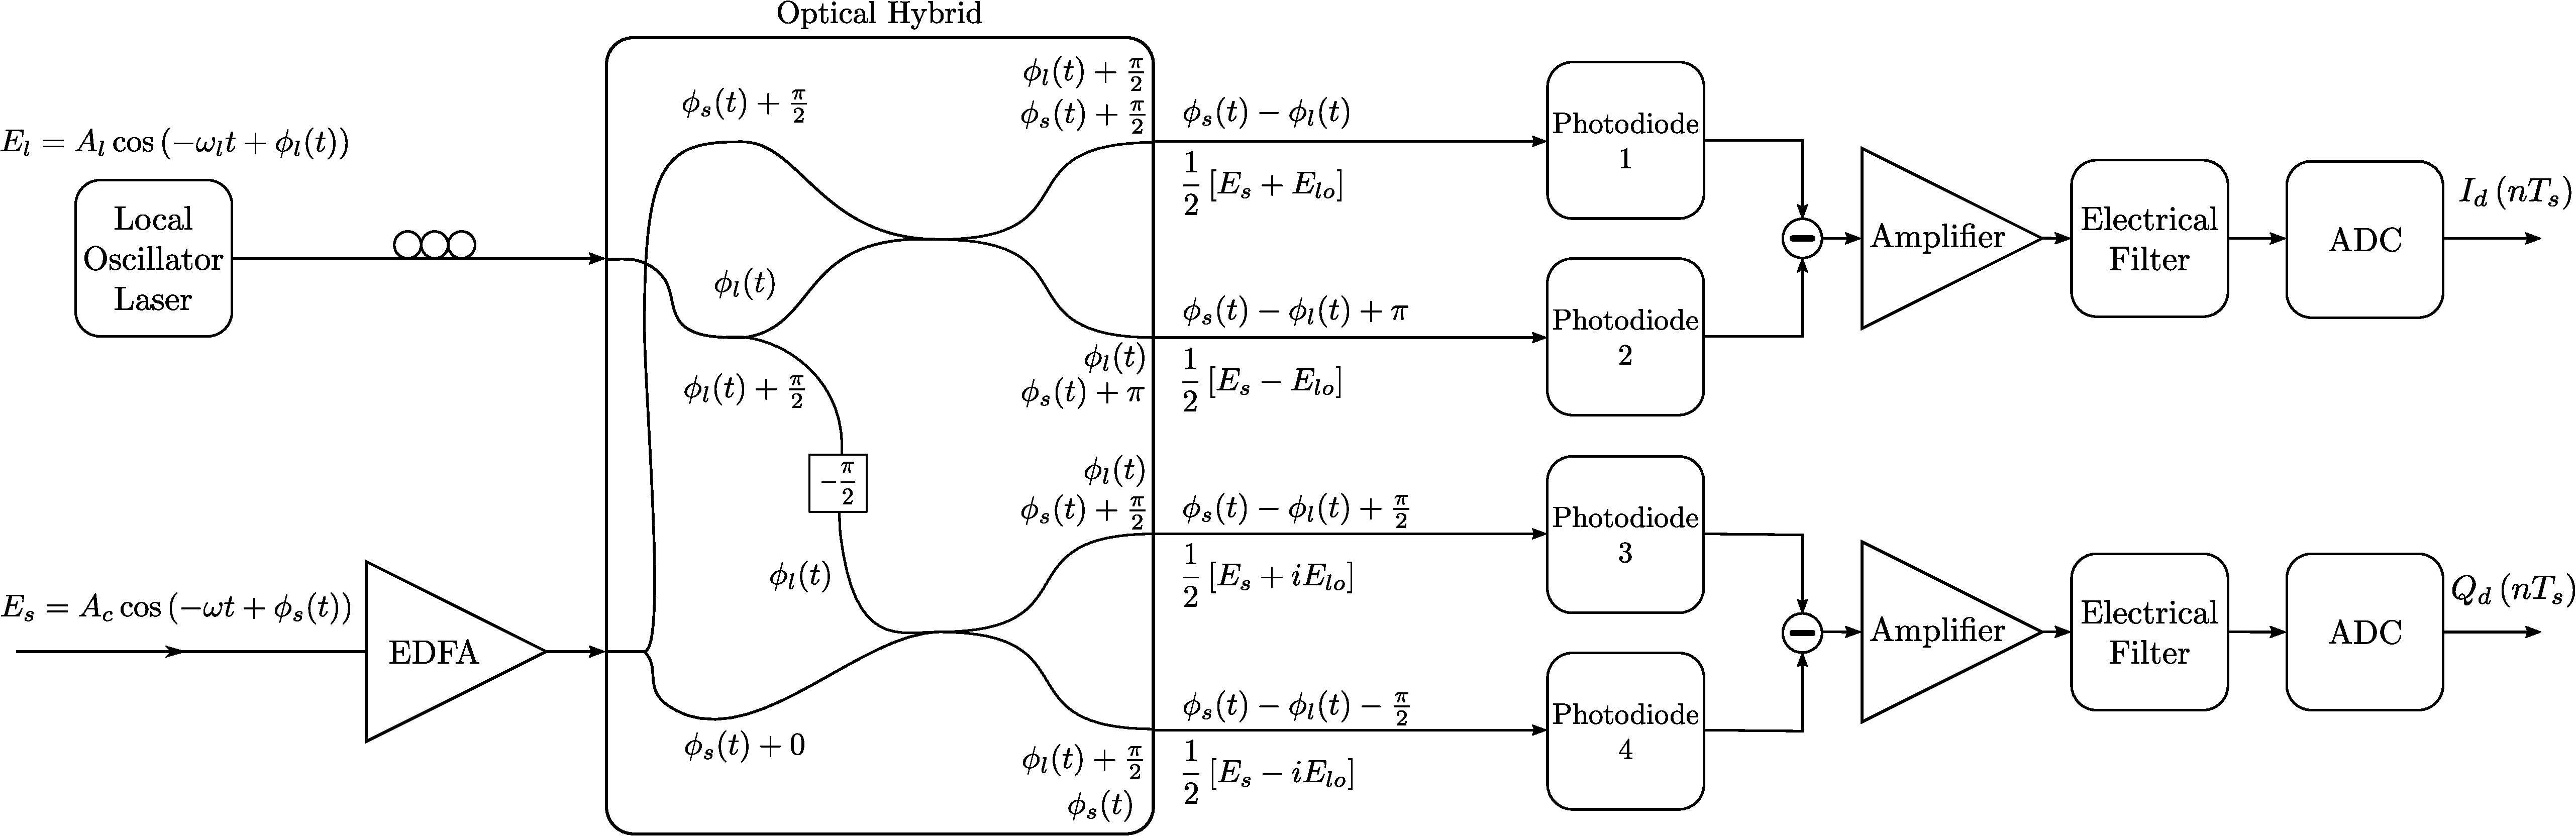
\includegraphics[width=0.95\textwidth]{./sdf/m_qam_system/figures/rxDiagramTeor_edfa.pdf}
		\caption{\label{fig:rxDiagram} Local oscillator and receiver filters
		diagram. $\phi_a$ and $\phi_b$ represent the phase rotations happening
	inside the optical hybrid.}
	\end{figure}

	Before starting, we should clarify how the optical hybrid works. A possible
	configuration is shown in Figure~\ref{fig:rxDiagram}, where the mixing is
	achieved resorting to a few directional couplers. Figure~\ref{fig:coupler}
	shows an example of a directional coupler, where two fiber cores are close enough so that the space
	between them is comparable to their diameter. In these conditions, the
	fundamental modes propagating through each fiber overlap partially, leading to
	power transfer from one core to the other~\cite{agrawal04}.

	\begin{figure}[H]
		\centering
		\centering
		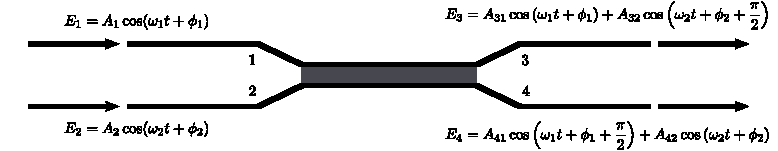
\includegraphics[width=0.95\textwidth]{./sdf/m_qam_system/figures/coupler.pdf}
		\caption{\label{fig:coupler} Directional coupler diagram.}
	\end{figure}

%	Consider the ratio between output and input power to be given by $\rho =
%	P_{o}/P_{i}$. The transfer matrix of a coupler following that relation is:
%
	Assuming a lossless directional coupler as shown Figure~\ref{fig:coupler},
	the relation between input and output power is:

	\begin{equation}\label{eq:couplerPower}
		P_1 + P_2 = P_3 + P_4
	\end{equation}


	With this in mind, the amplitudes $A_3$ and $A_4$
	on the output of a coupler are related to their inputs $A_1$ and $A_2$ by the
	coupling length $L$ and the coupling coefficient $k$:

	\begin{equation}\label{eq:couplerInOut}
	\begin{bmatrix}
		A_3 \\
		A_4 \\
	\end{bmatrix}
	=
	\begin{bmatrix}
		\cos(kL) & i\sin(kL) \\
		i\sin(kL) & cos(kL) \\
	\end{bmatrix}
	\begin{bmatrix}
		A_1 \\
		A_2 \\
	\end{bmatrix}
\end{equation}
% Considering an input on port 1, indicated on the diagram as $E_1$, the relation
% between the power at that point and at ports 3 and 4 is:
%
% \begin{align}
%	 P_3 (L_c) &= P_1 \cos^2(k_cL_c) \\
%	 P_4 (L_c) &= P_1 \sin^2(k_cL_c)
% \end{align}

Two things can be noticed here: first, the power ratios are dependent on the coupling
 length. This comes from the supermodes of the fiber coupler, which have
 different propagation constants~\cite{agrawal04}. This difference creates a relative phase shift
 proportional to the coupler length. In addition, a phase shift of $\pi/2$
 exists always between the two outputs. This is because the supermodes are the
 even and odd combinations of the fundamental modes of the coupler.

 This phase shift can be taken advantage of to create an optical hybrid, by mixing
 the components in a way to end up with 4 different combinations of the signal
 and LO, having relative phase differences of $0, \pi/2, \pi$ and $3\pi/2$.

% The power dependece comes from the supermodes of the fiber coupler, which have
% different propagation constants. Assuming the coupler to be symmetric, the
% modes are the even and odd combinations of the fundamental modes.
%
% both modes excited, a relative phase difference exists due to the different
% propagation constants of the modes. In addition, as the fi



%	Consider the ratio between output and input power to be given by $\rho =
%	P_{o}/P_{i}$. The transfer matrix of a coupler following that relation is:
%
%	The amplitudes $A_3$ and $A_4$ on the output of a coupler are related to their
%	inputs A_1 and A_2 by the coupling length L and the coupling coefficient k:
%
%	\begin{equation}
%	\begin{bmatrix}
%		A_3 \\
%		A_4 \\
%	\end{bmatrix}
%	=
%	\begin{bmatrix}
%		\cos(kL) & i\sin(kL) \\
%		i\sin(kL) & cos(KL) \\
%	\end{bmatrix}
%	\begin{bmatrix}
%		A_1 \\
%		A_2 \\
%	\end{bmatrix}
%\end{equation}

	We can now proceed to analyze the process at the receiver, but for now we will
	ignore the noise added by the EDFA shown at the beginning of the
	diagram.

	Coherent detection takes the product of the electric fields from the signal and
	a Local Oscillator, in order to measure the phase difference between them
	through interference. The electric field of the Local Oscillator
	is~\cite{kikuchi16}:

	\begin{equation}
		%E_{lo} = A_{lo} e^{i(-\omega_{lo} t + \phi_{lo})}
		E_{lo} = A_{lo} \cos{(-\omega_{lo} t + \phi_{lo})}
	\end{equation}

	The amplitudes $A_{lo}$ and $A_c$ are related to their respective average optical power by:

	\begin{align*}
		P_s    &= k {E_s}^2    = k {A_c}^2 \cos^2(-\omega t + \phi_s) = k
		\frac{{A_c}^2}{2} = k \frac{{(A \sqrt{2})}^2}{2} = k A^2 \\
		P_{lo} &= k {E_{lo}}^2 = k {A_{lo}}^2 \cos^2(-\omega_{lo} t + \phi_{lo}) = k \frac{{A_{lo}}^2}{2}
	\end{align*}

	\noindent where $k$ is the ratio between the effective beam area and the impedance of free
	space. The power of the signal entering the EDFA is amplified by a gain factor $G_o$

	\begin{equation}
		P_{\text{s\_out}} = G_o P_{\text{s\_in}}
	\end{equation}

	\noindent	$G_o$ is the EDFA optical gain, given by~\cite{mukai81}:

	\begin{equation}\label{fig:ampGain}
		G_o = \frac{G_\text{small}}{1+\frac{P_\text{in}}{P_{\text{sat}}}}
	\end{equation}

	\noindent where $G_\text{small}$ is the gain for small signals, $P_\text{in}$ is
	the optical power at the EDFA's input and $P_\text{sat}$ is the EDFA's
	saturation power. This means that the effective optical gain is lower for
	input signals with higher optical powers.


	As the input optical signal and local oscillator enter the optical hybrid,
	each of them is split twice in 3-dB couplers. This means that a quarter of the
	power from each source reaches each of the photodiodes. In addition, as
	previously explained, they are subject to phase shifts which mix them with
	differente relative phase differences.
	We therefore get 4 different combinations from $E_s$ and$E_{lo}$, the
	electrical fields of the signal and the LO.

	\begin{align*}
		E_1 &= \frac{1}{2}\left(\sqrt{G_o} E_s + E_{lo}\right) \\
		E_2 &= \frac{1}{2}\left(\sqrt{G_o} E_s - E_{lo}\right) \\
		E_3 &= \frac{1}{2}\left(\sqrt{G_o} E_s + i E_{lo}\right) \\
		E_4 &= \frac{1}{2}\left(\sqrt{G_o} E_s - i E_{lo}\right) \\
	\end{align*}

	Let us assume from now on that $\omega = \omega_{lo}$ and $\phi_{lo} = 0$. In
	this case, the photocurrent for the each of the previous n combinations is
	equal to:

%	\begin{align}
%		I_1 (t) &= \frac{R}{4} \left[ P_s(t) + P_{lo} + 2 \sqrt{P_s(t)P_{lo}}
%						\cos{(\phi_s(t) - \phi_{lo}(t))}\right] \\
%		I_2 (t) &= \frac{R}{4} \left[ P_s(t) + P_{lo} - 2 \sqrt{P_s(t)P_{lo}}
%						\cos{(\phi_s(t) - \phi_{lo}(t))}\right] \\
%		I_3 (t) &= \frac{R}{4} \left[ P_s(t) + P_{lo} + 2 \sqrt{P_s(t)P_{lo}}
%						\sin{(\phi_s(t) - \phi_{lo}(t))}\right] \\
%		I_4 (t) &= \frac{R}{4} \left[ P_s(t) + P_{lo} - 2 \sqrt{P_s(t)P_{lo}}
%						\sin{(\phi_s(t) - \phi_{lo}(t))}\right] \\
%	\end{align}

	\begin{align}
		I_1 (t) &= \frac{\eta}{4} \left[ G_o P_s(t) + P_{lo} + 2 \sqrt{G_o P_s(t)P_{lo}}
						\cos{\big(\phi_s(t)\big)}\right] \\
		I_2 (t) &= \frac{\eta}{4} \left[ G_o P_s(t) + P_{lo} - 2 \sqrt{G_o P_s(t)P_{lo}}
						\cos{\big(\phi_s(t)\big)}\right] \\
		I_3 (t) &= \frac{\eta}{4} \left[ G_o P_s(t) + P_{lo} + 2 \sqrt{G_o P_s(t)P_{lo}}
						\sin{\big(\phi_s(t)\big)}\right] \\
		I_4 (t) &= \frac{\eta}{4} \left[ G_o P_s(t) + P_{lo} - 2 \sqrt{G_o P_s(t)P_{lo}}
						\sin{\big(\phi_s(t)\big)}\right] \\
	\end{align}

	\noindent where $\eta$ is the photodiodes' responsivity.
	Two photocurrents are generated from the combination of the balanced photodiodes,
	which are then amplified in a transimpedance amplifier with a gain factor $G_e$.

	\begin{align}
		V_i(t) &= G_e\left(I_{1} - I_{2}\right) \notag\\
					 &= G_e \eta \sqrt{G_o P_s P_{lo}} \cos{(\phi_{s}(t))} \label{eq:photocurrentI} \\
		V_q(t) &= G_e\left(I_{3} - I_{4}\right) \notag\\
					 &= G_e \eta \sqrt{G_o P_s P_{lo}} \sin{(\phi_{s}(t))}\label{eq:photocurrentQ}
	\end{align}

	These voltages effectively reconstruct the transmitted optical signal.
	After going through the electrical filter, they can be sampled
	into the digital domain for processing.

	Assuming perfect synchronization, if the signal is sampled with timing $t =
	n T_s$, the constellation can be reconstituted perfectly, if there is no
	intersymbol interference. In this case, according to
	equations~\ref{eq:pulsesi} and~\ref{eq:pulsesq}, $p_i(t)$ and $p_q(t)$ are
	equal to either $1$ or $-1$. It follows that $\phi_s(t = nT_s) = \frac{\pi}{4}
	\pm m \frac{\pi}{2}$. If the gain $G_e$ is adjusted so that $ G_e\eta\sqrt{G_o P_s
	P_{lo}} = A_c$, we get:

	\begin{align}
		V_i(t) &= {A_c} \cos{(\phi_{s}(t))}, \notag \\
					 &= \pm \frac{A_c}{\sqrt{2}} = \pm A_i = \pm A \qquad t = nTs \label{eq:rxSymbolsi} \\
		V_q(t) &= {A_c} \sin{(\phi_{s}(t))}, \notag \\
					 &= \pm \frac{A_c}{\sqrt{2}} = \pm A_q = \pm A \qquad t = nTs \label{eq:rxSymbolsq}
	\end{align}


%	\begin{equation}
%		\begin{split}
%			I (t) &= I_i(t) + I_q(t) \\
%						&= G R \sqrt{P_s P_{lo}}
%		\left[\cos{(\phi_s(t))}+\sin{(\phi_s(t))}\right] \\
%						& = \frac{A_c}{\sqrt{2}}
%		\left[\cos{(\phi_s(t))}+\sin{(\phi_s(t))}\right]
%		\end{split}
%	\end{equation}


	Looking at Figure~\ref{fig:rxConst}, we can see that
	equations~\ref{eq:rxSymbolsi} and~\ref{eq:rxSymbolsq} describe the four points in the
	constellation.

	\begin{figure}[H]
		\centering
		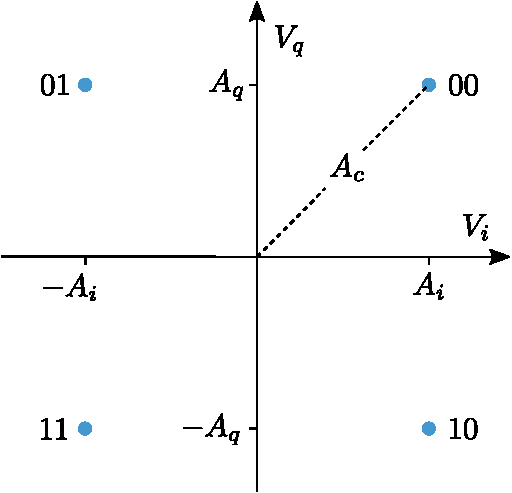
\includegraphics[width=0.5\textwidth]{./sdf/m_qam_system/figures/constellationRx.pdf}
		\caption{A QPSK constellation, assuming $ A = A_i = A_q =
			A_c/\sqrt{2}$.\label{fig:rxConst}}
	\end{figure}

	The previous explanation assumes that the polarization of both the transmitted
	signal and the local oscillator is aligned. This can be achieved by using a
	polarization controller, as shown in Figure~\ref{fig:rxDiagram}. We have also
	neglected any link losses.

	\subsubsection{ISI}\label{sec:ISI}
	We have assumed the absence of intersymbol interference.
	As previously mentioned, bits are coded into the symbols of a given constellation.
	These symbols, associated with a given discrete amplitude, need to be
	encoded into the I and Q carriers. For this, a given shape must be used to
	translate the discrete symbols into continuous, finite pulses in the analog domain.
	The choice of the shape to be used is particularly important for the ISI.

	\begin{figure}[b]
		\centering
		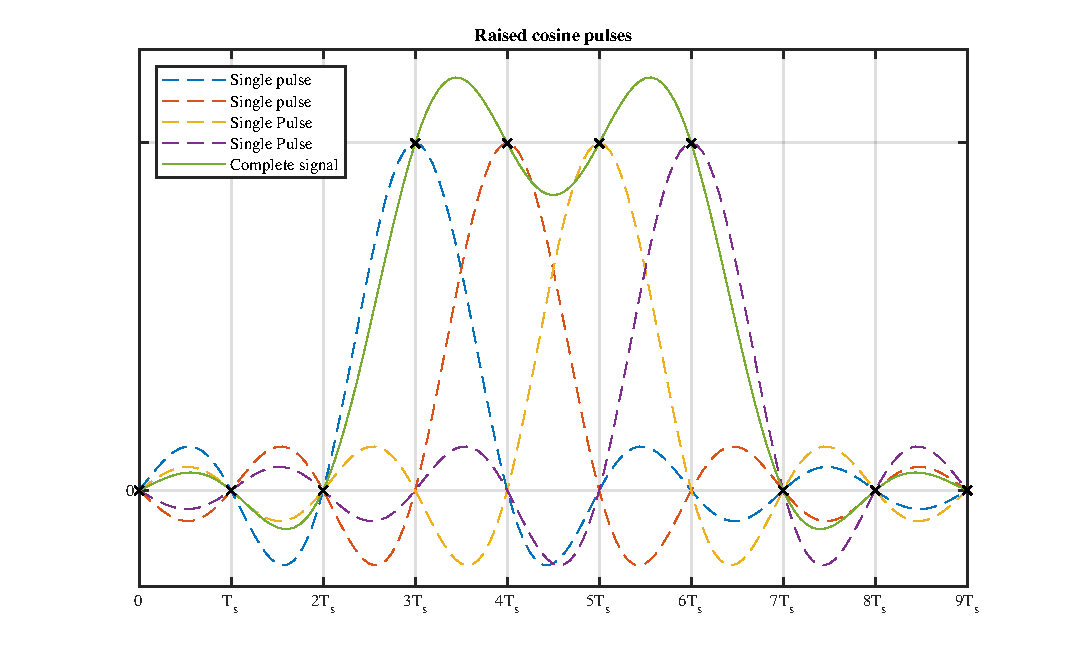
\includegraphics[width=\textwidth]{./sdf/m_qam_system/figures/eyes/ISI/signalAndPulsesRaisedCosine.pdf}
		\caption{Signal generated by four sequential raised cosine pulses. It can be seen
		that at $t=nT_s$, every pulse except one equals exactly zeros, showing that
	there is no interference. In addition, at those times, the value of the signal
is coincident with the peak of the individual pulses.}
\label{fig:ISIRCsig}
	\end{figure}

	Each symbol is represented by its own pulse, which is dependent on the symbol
	period $T_s$. In each pulse, there is an optimal instant $t_s$, where we can sample the signal in
	order to perfectly identify the contained symbol. These instants are separated by a time
	equal to the symbol period. In order to negate intersymbol interference, the
	signal for each pulse should be equal to zero every time a different symbol is
	sampled, that is, at all instants $t_s \pm nT_s$. If this condition is verified,
	the value of the signal at $t=t_s$ is dependent only on the symbol transmitted
	at that time, not being influenced by the surrounding pulses. This is shown in
	Figure~\ref{fig:ISIcomp}, where we can see that at all instants $nT_s$, the
	reponse is zero for all pulses but one. Consequently, at those instants, the
	signal obtained from the combination of all pulses is exactly equal to the peak
	of the pulse transmitted at that time. Those instants are also shown at the
	center of the eye diagram shown in Figure~\ref{fig:ISIcomp}, where $t_s$ is
	represented, and perfect coincidence in the signal at sampling time is shown.

	The raised-cosine is a shape commonly used for pulse shaping, as it does not
	create any intersymbol interference. This is shown in
	Figure~\ref{fig:ISIcomp}. The time domain response for raised-cosine filter is
	given by~\cite{nguyen09}

	\begin{equation} \label{eq:rcTD}
		h_{RC}(t) = \frac{\sin(\pi t/ T_s)}{(\pi t/ T_s)} \frac{\cos(\pi \beta t
		/T_s)}{1-(4\beta^2 t^2/T_s^2)}
	\end{equation}

	\noindent where $\beta$ is the roll-off factor and $T_s$ is the symbol period.

	\begin{figure}
		\centering
		\begin{minipage}{0.45\textwidth}
			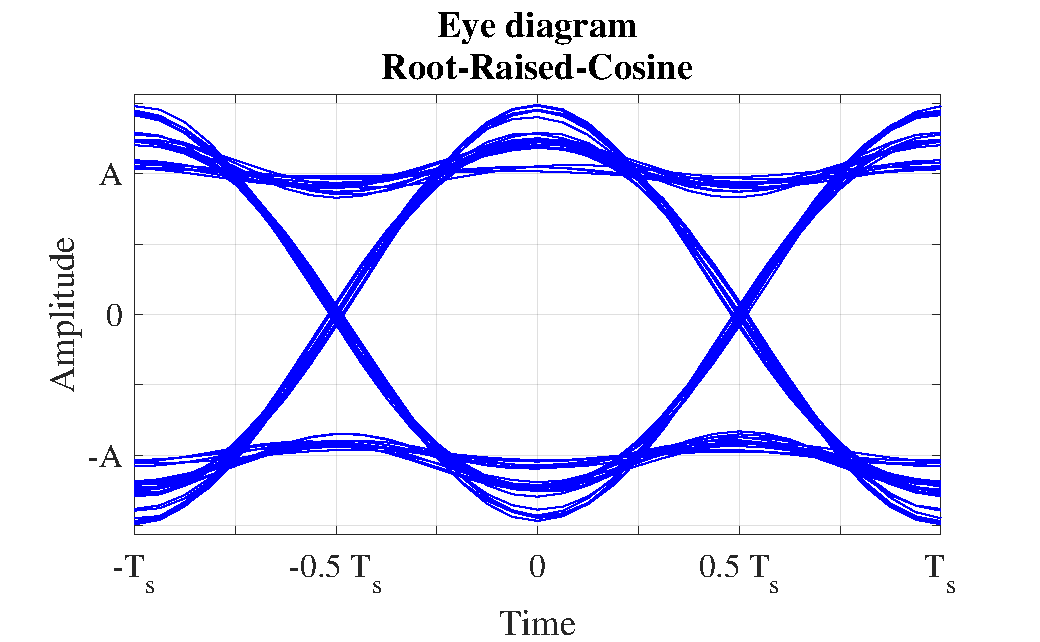
\includegraphics[width=\textwidth]{./sdf/m_qam_system/figures/eyes/ISI/RRC.pdf}
		\end{minipage}
		\begin{minipage}{0.45\textwidth}
			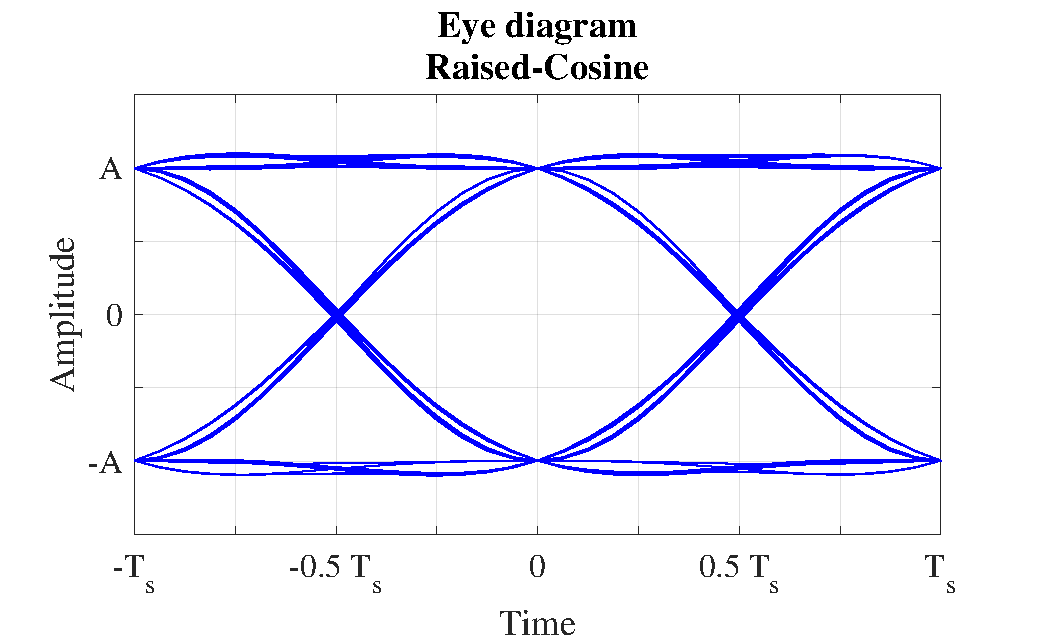
\includegraphics[width=\textwidth]{./sdf/m_qam_system/figures/eyes/ISI/RC.pdf}
		\end{minipage}
		\caption{Eye diagrams of two signals without noise: on the left,
			shaped with a single root-raised-cosine filter and affected by ISI; on the right,
		shaped using a raised-cosine filter, showing no signs of ISI.}
		\label{fig:ISIcomp}
	\end{figure}

%	\begin{figure}[H]
%		\centering
%		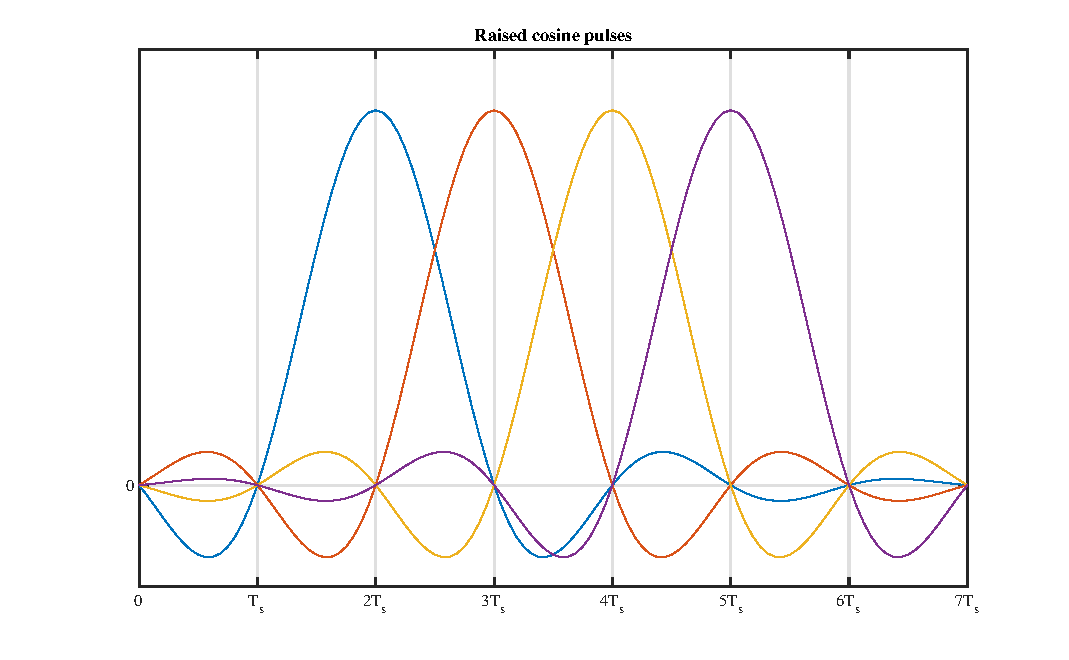
\includegraphics[width=\textwidth]{./sdf/m_qam_system/figures/eyes/ISI/pulsesRaisedCosine.pdf}
%		\caption{Sequence of four raised-cosine pulses. It can be seen that at $t=nT_s$,
%		every pulse equals zero except one, which will have its maximum value there.}
%		\label{fig:ISIcomp}
%	\end{figure}


	Optimal detection often requires the implementation of matched
	filters~\cite{schwartz90}. This is because in addition to avoiding ISI, it is
	desirable to maximize the SNR before sampling the signal, and in order to achieve
	both these objectives simultaneously, a matched filter should be used. This is
	done by
	implementing in the receiver a filter similar to the one used to initially
	shape the pulses. The pulse-shaping process becomes divided between the
	transmission and reception stages. Provided that an approppriate filter is
	chosen, the resulting signal can still be free of ISI, while reducing the
	noise power in the final sampled signal.

	The first filter, implemented on the transmitter, will convert the discrete
	symbols into continuous shapes, so that it can be transmitted on a modulated
	signal. The filter at the receiver finalizes the shaping process, making the
	signal reach the desired shape for symbol identification. In addition, it
	decreases the amount of noise affecting the signal.

	With matched filtering, the raised-cosine can be implemented by having the
	filters at the transmitter and receiver be root-raised-cosine filters.
	The end result will be signal with the same shape as if a raised cosine
	filter were used at the transmitter.

	The root-raised-cosine is defined as a filter for which the square of the
	frequency response is equal to the frequency response of the raised cosine
	filter. Its time domain impulse response
	given by\cite{nguyen09}:

	\begin{equation}\label{eq:rrcTD}
		h_{RRC}(t) = \frac{(4\beta t/T_s)\cos\big[\pi(1+\beta)t/T_s\big] +
		\sin\big[\pi(1-\beta)t/T_s\big]}
		{(\pi t/T_s)\big[1-(4 \beta t/T_s)^2\big]}
	\end{equation}

%	Having a signal pass through the same root-raised-cosine filter twice is equivalent
%	has having it pass a raised-cosine filter.

	\subsubsection{Noise}
	So far we have neglected to include any source of noise in this analysis.
	Several possible noise sources can be considered, either in the optical
	or in the electrical part of the system. As shown in
	Figure~\ref{fig:rxDiagram}, for now we will only consider the existence of
	optical noise,  and we will consider that the noise added is ASE which could
	originate from a EDFA. The ASE field can be represented as a sum of terms as
	follows ~\cite{crognale14, olsson89}:

	\begin{align}
		E_{\text{ASE}x} &= \sum_{k=-B_\nu}^{B_\nu} \sqrt{2 n_{0o} \delta \nu}
		\cos{((-\omega + 2\pi k \delta \nu) t + \phi_{kx})} \\
		E_{\text{ASE}y} &= \sum_{k=-B_\nu}^{B_\nu} \sqrt{2 n_{0o} \delta \nu}
		\sin{((-\omega + 2\pi k \delta \nu) t + \phi_{ky})}
	\end{align}

	\noindent where $B_\nu = B_{\text{opt}}/(2 \delta \nu)$, $B_{\text{opt}}$ is the optical
	bandwidth and $\delta \nu$ is small frequency interval. We can write an
	expression for the optical noise spectral density $n_{0o}$ considering the use of a number
	$N_A$ of cascaded EDFA's. Assuming that all amplifiers are similar and equally
	spaced, and that the gain in each EDFA is just enough to compensate the fiber
	losses in the distance between them, we have~\cite{agrawal12}:

	\begin{equation}
		n_{0o} = N_A n_{\text{sp}} (G_o-1) h\nu
	\end{equation}

	Here, $n_{\text{sp}}$ is the EDFA's spontaneous emission factor, $h\nu$ is the
	photon energy.
	In additon, $\phi_{kx}$ and $\phi_{ky}$ are independent uniform random
	variables representing random phases for each of the terms in the summation,
	and $G_o$ is the amplifiers'  optical gain as defined in
	equation~\ref{fig:ampGain}.
	This field is added to equation~\ref{eq:sigEq}, giving rise to three noise
	terms from different interactions:

	\begin{itemize}
		\item ASE-LO, from the interaction with the local oscillator;
		\item ASE-SIG, from the interaction with the transmitted signal;
		\item ASE-ASE, from the interaction with itself.
	\end{itemize}

	For now, we will consider only the ASE-LO component, which  is close enough
	to additive white Gaussian noise. In addition, it is typically the strongest,
	as usually the LO power is much greater than either the signal or the ASE. The
	variance, or noise power, generated by this component at each pair of balanced
	photodiodes is given by~\cite{crognale14}:

%		\sigma_{\text{ASE}-\text{SIG}}^2 &= 2 \eta^2 \alpha P__s P_{\text{LO}} n_{0o} B_N \\
%		\sigma_{\text{ASE}-\text{ASE}}^2 &= \sqrt{2} \eta P_{\text{LO}} n_{0o} B_N \\
	\begin{equation}\label{eq:noiseComps}
		\sigma_{\text{ASE}-\text{LO}}^2 = 2 \eta^2 P_{\text{LO}} n_{0o} B_N =
		2 \eta^2 P_{\text{LO}} N_A n_{\text{sp}} (G_o - 1) h\nu B_N
	\end{equation}

	\noindent Here, $B_N$ is the electrical noise bandwidth. Notice that the total noise
	power is proportional to this bandwidth, so keeping it closer to the signal's
	bandwidth limits the total noise to a minimum. This noise is also amplified at
	the transimpedance amplifier, so we get a voltage variance equal to:

	\begin{equation}\label{eq:noiseCompsAmp}
		\sigma_{\text{ASE}-\text{LO}}^2 = 2 \eta^2 G_e^2 P_{\text{LO}} N_A n_{\text{sp}} (G_o - 1) h\nu B_N
	\end{equation}

	Considering the generated noise to be independent from the signal, let $x(t)$
	be the signal at the ADCs, sampled at a given instant $t$ for either the
	in-phase or quadrature component. $x(t)$ has two components:

	\begin{equation}\label{eq:sampledComponents}
		x(t) = s(t) + n(t)
	\end{equation}

	\noindent where the component $s(t)$ corresponds to the received signal, and
	$n(t)$ corresponds to the noise component. For $t = nT_s$, as mentioned in
	equations~\ref{eq:rxSymbolsi} and~\ref{eq:rxSymbolsq}, $s(t) = \pm A$. The
	noise component, being AWGN, has constant power spectral density, and follows
	a Gaussian distribution with zero mean and variance equal to the noise power
	as described in equation~\ref{eq:noiseCompsAmp}.

	It's possible to remove the exceeding noise through filtering. This is
	done by the matched filter, as mentioned in the previous
	section. The filter essentially decreases the bandwidth, removing all
	the noise at frequencies not contained in $f < \big|{1}/{(2T_s)}\big|$, while
	not causing intersymbol interference in the transmitted signal.

	Let us consider a signal as described in
	Equation~\ref{eq:sampledComponents}, with $ a(t) = A_p~p(t) $, where $A_p$ is the peak
	amplitude of the signal and $p(t)$ is the shape of the pulse. In addition, let $n(t)$ be AWGN
	of spectral density $G_n(f) = {n_0}/{2}$. Finally, assume that the filter
	at the receiver has a frequency response $H(f)$.
	The filter is similar to the shape of the pulse , but reversed in time and
	shifted by a time delay, such that it maximizes the SNR~\cite{carlson86}.
	The energy contained in the pulse that enters the receiver filter depends on the
	pulse amplitude and on its shape, and it is given by:
%
	\begin{eqnarray}\label{eq:pulseEnergy}
		E_p = \int_{-\infty}^{\infty} {|A(f)|}^2 df = A_p^2 \int_{-\infty}^{\infty} {|P(f)|}^2 df
	\end{eqnarray}

	The amplitude of the signal component after the receiver filter $H(f)$, at a
	given sampling time $t=t_0+t_d$, is:

	\begin{eqnarray}
		A = \mathfrak{F}^{-1}\left[H(f) A(f)\right]\big|_{t=t_0+t_d} = A_p \int_{-\infty}^{+\infty} H(f) P(f) e^{+j \omega t_d}df
	\end{eqnarray}

	Similarly, the noise power at the receiver filter output is given by:

	\begin{eqnarray}
		N_o = \int_{-\infty}^{+\infty} {|H(f)|}^2 G_n(f) df = \frac{n_0}{2} \int_{-\infty}^{+\infty} {|H(f)|}^2
	\end{eqnarray}

	This means that the peak signal power to mean noise power ratio at the filter
	output is given by:

	\begin{eqnarray}
		\frac{A^2}{N_o} &= A_p^2 \frac{\big|\int_{-\infty}^{+\infty} |H(f) P(f)e^{j\omega t_d} df\big|^2}{\int_{-\infty}^{+\infty} {|H(f)|}^2 G_n(f) df}\\\nonumber
											&= A_p^2 \frac{\big|\int_{-\infty}^{+\infty} |H(f) P(f)e^{j\omega t_d} df\big|^2}{\frac{n_0}{2}\int_{-\infty}^{+\infty} {|H(f)|}^2df}
	\end{eqnarray}

	It can be shown that a matched filter maximizes the ratio above, so that it
	becomes~\cite{carlson86} :

	\begin{equation}
		\frac{A^2}{N_o} = \frac{A_p^2}{n_0/2} \int_{-\infty}^{+\infty} |P(f)|^2 df = \frac{A_p^2}{n_0/2} \int_{-\infty}^{+\infty} p(t)^2 dt
	\end{equation}

%
%	This shows that the SNR and, therefore, the error probability after filtering is dependent on
%	the energy of each symbol and the noise spectral density. However, even though
%	the relation does not directly depend on the pulse shape, the energy of each
%	symbol still depends on the pulse shape. The energy of the symbol results from
%	an integration over the symbol period.


%	It can be
%	shown~\cite{carlson86} that, according to what has been shown so far

	Thus, substituting from equation~\ref{eq:pulseEnergy}, the following relation
	can be verified for the signal after the matched filter:

	\begin{equation}\label{eq:amp2en}
		\frac{A^2}{N_o} = \frac{2 E_b}{n_0}
	\end{equation}

	Here, $A$ is the amplitude of $s(t)$ at the output of the matched filter,
	$N_o$ is the corresponding noise power, $E_b$ is the energy per bit and $n_0/2$
	is the two-sided noise spectral density, obtained from
	equation~\ref{eq:noiseCompsAmp} from
	$n_0 = \sigma_{\text{ASE}-\text{LO}}^2 / B_N$.


	$x(t) = s(t) + n(t)$ remains a valid representation of the signal for each of
	the quadratures after the matched filter, even if $s(t)$ and $n(t)$ have
	changed. In addition, $n(t)$ remains additive Gaussian noise. Therefore,
	$x(t)$ after the matched filter, at time $t = nT_s$ is also a Gaussian random
	variable, and has mean $A^2$ and variance $N_o$. This relation will show
	itself useful during the analysis of the error probability in the following
	section.


	\subsubsection{Bit error rate}
	For each quadrature, an error occurs in one of two situations: when a 0 is
	transmitted but a 1 is identified, or a 1 is transmitted and a 0 is
	identified.

	As previously mentioned, the values sampled at sampling time $t = nT_s$, which are used to
	identify the received symbols, follow a Gaussian
	distribution. Using the constellation from
	Figure~\ref{fig:const_2m}, with a decision boundary halfway between $A$ and
	$-A$, an error occurs in two situations:

	\begin{equation}
		\begin{cases}
			x(t) < 0, \quad \text{if } s(t)=A \\
			x(t) > 0, \quad \text{if } s(t)=-A
		\end{cases}
		\implies \quad
		\begin{cases}
			n(t) < -A, \quad \text{if } s(t)=A \\
			n(t) > A, \quad \text{if } s(t)=-A
		\end{cases}
	\end{equation}

	This is illustrated in Figure~\ref{fig:gauss},
	where the probability of error is shown by the colored area under the
	curves~\cite{schwartz90}.

	\begin{figure}[]
		\centering
		\begin{minipage}{1\textwidth}
			\centering
			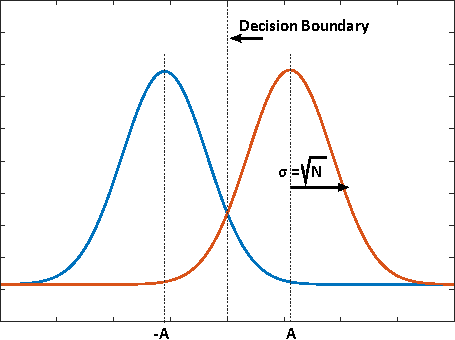
\includegraphics[width=0.50\textwidth]{./sdf/m_qam_system/figures/gaussians.pdf}
			\subcaption{}
		\end{minipage}
		\begin{minipage}{0.35\textwidth}
			\centering
			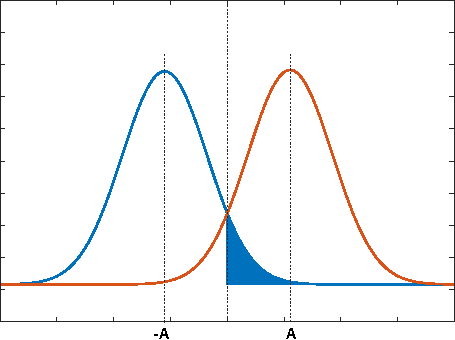
\includegraphics[width=1\textwidth]{./sdf/m_qam_system/figures/gaussian_error_blue.pdf}
			\subcaption{}
		\end{minipage}
		\begin{minipage}{0.35\textwidth}
			\centering
			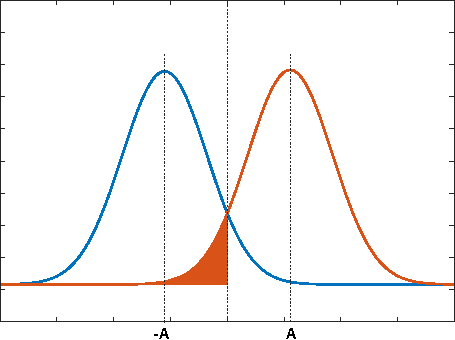
\includegraphics[width=1\textwidth]{./sdf/m_qam_system/figures/gaussian_error_orange.pdf}
			\subcaption{}
		\end{minipage}
		\caption{Probability density functions for $x(t) = s(t) + n(t)$, with
		$s(t)=\pm A$ at the time of sampling, and $n(t)$ as a Gaussian variable of
	zero mean and variance $N$. The colored areas below the curves on the right
represent the probability of error for each transmitted bit.}
		\label{fig:gauss}
	\end{figure}

	The probability of bit error (assuming equal emission probabilities for both bits) can be expressed as:

	\begin{equation}
		\begin{split}
			P_{be} &= P_0 P_{e0} + P_1 P_{e1} = \frac{1}{2} P_{e0} +
			\frac{1}{2} P_{e1} \\
						 &= \frac{1}{2} \Bigl[\Pr\Bigl(n(t)<-A\Bigr) +
						 \Pr\Bigl(n(t)>A\Bigr)\Bigr]
		\end{split}
	\end{equation}

	$P_0$ and $P_1$ are the probabilities of the transmitted bit being a 0 or
	1, respectively, and $P_{e0}$ and  $P_{e1}$ are the respective probabilities of
	error. It follows that the probability of bit error can be described using the
	Q-function, or alternatively, the complementary error function.

	\begin{equation}\label{eq:berMQAM}
		P_{be} =  Q\left({\frac{A}{\sqrt{N_o}}}\right) = \frac{1}{2}
		\text{erfc}\left({\frac{A}{\sqrt{2 N_o}}}\right)
	\end{equation}

	The probability of bit error is also known as bit error rate, or BER.

	We have worked on the probability of bit error for each
	quadrature independently. However, assuming a gray code, and knowing that the
	carriers are uncorrelated, an error in each carrier is independent from the
	other~\cite{nguyen09}. This can be verified by noting that the even bits are
	dependent only on one of the quadratures, and the odd bits depend on the
	other. Therefore, as half the bits are even and half are odd, and assuming
	that the constellation is symmetrical, it follows that the error rate is the
	same as for each quadrature independently.

	\begin{equation}
		\begin{split}
			\text{BER} &= P_{\text{odd}} P_{\text{oddError}} +
								 P_{\text{even}}P_{\text{evenError}}\\
								 &= \frac{1}{2} P_{\text{oddError}} + \frac{1}{2}
								 P_{\text{evenError}}\\
								 &= \frac{1}{2} \left(Q\left({\frac{A_{even}}{\sqrt{N_{even}}}}\right)
								 +Q\left({\frac{A_{odd}}{\sqrt{N_{odd}}}}\right) \right)\\
								 &= Q\left({\frac{A}{\sqrt{N_o}}}\right)
		\end{split}
	\end{equation}


	Looking back at equation~\ref{eq:amp2en}, we can also define the probability
	of error as a function of the energy per bit:

	\begin{equation}\label{eq:berMod}
		P_{be} =  Q\left(\sqrt{\frac{2 E_b}{{n_0}}}\right) = \frac{1}{2} \text{erfc}\left(\sqrt{\frac{E_b}{n_0}}\right)
	\end{equation}

	While the BER can be calculated by analyzing each quadrature independently,
	the probability of symbol error is different. In this case, a symbol error
	happens whether there is an error in one of the quadratures or in both. There
	is no distinction between these cases. Therefore, the calculation of the
	symbol error rate requires a different approach. Let us first define the
	probability of correctly identifying a symbol.

	\begin{equation}
		P_C = (1 - P_{be})^2
	\end{equation}

	From this, the probability of symbol error is:

	\begin{equation}
		\begin{split}
			P_{Se}  &= 1-P_C \\
							&= 1 - \left(1 - Q \left({\frac{A}{\sqrt{N_o}}}\right)\right)^2
			\\
							&= 2 Q\left({\frac{A}{\sqrt{N_o}}}\right)\left[1-\frac{1}{2} Q
			\left({\frac{A}{\sqrt{N_o}}}\right)\right] \\
							&= 2 Q\left({\sqrt{\frac{2E_b}{{n_0}}}}\right)\left[1-\frac{1}{2}
			Q \left({\sqrt{\frac{2E_b}{{n_0}}}}\right)\right]
		\end{split}
	\end{equation}

	\begin{figure}
		\centering
		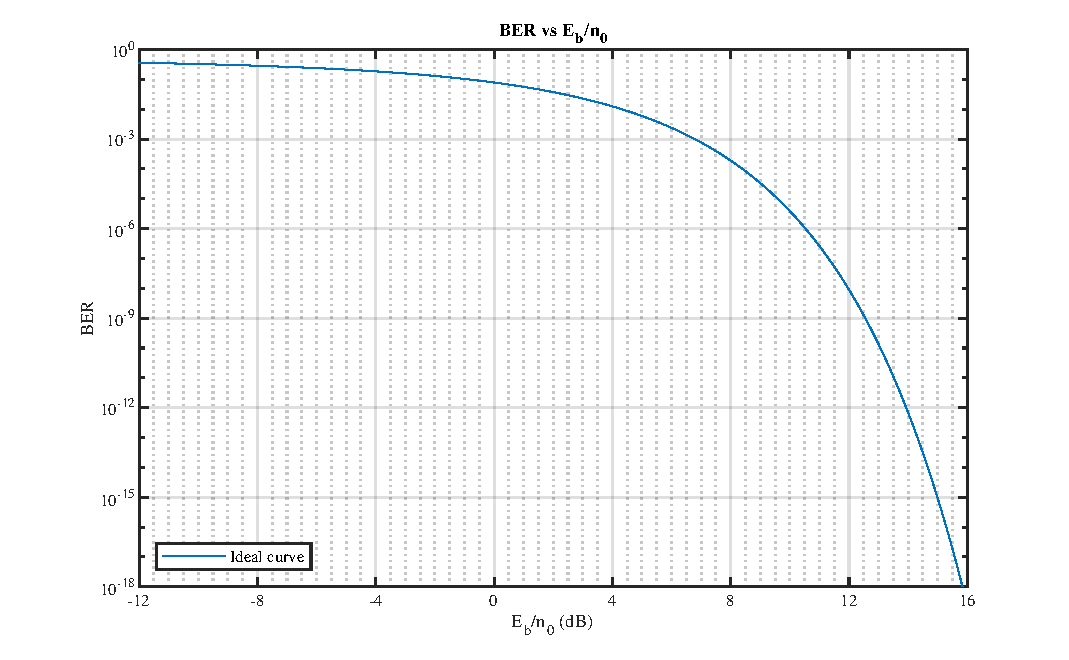
\includegraphics[
		width=1\textwidth]{./sdf/m_qam_system/figures/berPlots/ebn0Curve.pdf}
		\caption{QPSK theoretical BER curve as a function of the ratio of energy per
		bit and the noise spectral density in dB.\label{fig:QPSK_ebn0_curve}}
	\end{figure}

	It's worth noting that these equations are only valid for M=4, as in that case
	the system is similar to QPSK with a 4 point constellation. For $M > 4$ a
	different approach is required for calculating the BER, as the decision
	borders will be very different.

	We can now write the expected bit error rate as a function of the system
	parameters. To get $E_b$, we can start by picking up the equations for the
	signal waveforms which are sampled and measured at the ADC, described in
	Equations~\ref{eq:photocurrentI} and~\ref{eq:photocurrentQ}.

	\begin{equation}
		E_b(t) = G_e^2 \eta^2 {G_o P_s P_{lo}} \frac{T_s}{2} \label{eq:energyPerBit}
		%E_b(t) = G_e^2 \eta^2 {G_o P_s P_{lo}} \sin^2{(\phi_{s}(t))} \frac{T_s}{2} \label{eq:photocurrentQ}
	\end{equation}

	To get $n_0$, we start with equation~\ref{eq:noiseCompsAmp}, which gives the
	noise variance at the ADC's. The noise power spectral density will be the
	ration of this variance to the electrical bandwidth of the receiver. So we
	get:

	\begin{equation}\label{eq:sampledn0}
		\begin{split}
			n_0 &= \frac{2 \eta^2 G_e^2 P_{\text{LO}} N_A n_{\text{sp}} (G_o -
			1)h\nu B_N}{B_N} \\
					&= 2 \eta^2 G_e^2 P_{\text{LO}} N_A n_{\text{sp}} (G_o - 1) h\nu \\
					&= 2 \eta^2 G_e^2 P_{\text{LO}} n_{0o}
		\end{split}
	\end{equation}

\pagebreak
    %! TEX root = ../../main_netxpto.tex

	\subsection{Simulation Analysis}
	The M-QAM transmission system is a set of blocks that simulate the
	modulation, transmission and demodulation of an optical signal using M-QAM
	modulation. It is composed of several complex blocks: a transmitter, a
	receiver, a noise source, an addition block, a sink and a block that performs a Bit Error Rate (BER) measurement.
	The schematic representation of the system is presented in
	Figures~\ref{fig:sim_systemDiagram} to~\ref{fig:sim_rxDiagram}. The 
	simulation currently implements a QPSK system (M=4).

	\subsubsection{Functional description}
	A complete description of the M-QAM transmitter and M-QAM homodyne receiver
	blocks can be found in the \textit{Library} chapter of this document as well as
	a detailed description of the independent blocks that compose these blocks.
	The M-QAM transmitter generates one or two optical signals by encoding a binary
	string using M-QAM modulation. It also outputs a binary signal that is used to
	perform the BER measurement. The optical signal is then sent through a fiber 
	block, which attenuates it, simulating transmission over a given distance. 
	Aftwerwards, as EDFA block is present to be used as an optical preamplifier. 
	The amplified optical signal, with added ASE noise, is then sent to the 
	homodyne receiver.

	
	The homodyne receiver requires two optical inputs: one of the signal itself, 
	and another from a local oscillator perform the signal demodulation. It 
	receives, processes and decodes the received signal and afterwards outputs 
	the reconstructed bitstream. 
	This signal is compared to the binary signal generated by the
	transmitter in order to estimate the Bit Error Rate (BER).
	The files used are summarized in tables~\ref{tab:sources} and~\ref{tab:headers}.
	All the blocks and sub-blocks used are included in the tables.

	\begin{figure}[h]
		\centering
		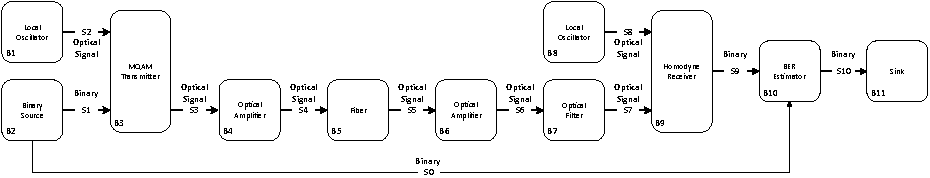
\includegraphics[width=1\textwidth]
			{./sdf/m_qam_system/figures/simulations/blockDiagrams/simulation_mqam}
		\caption{Top-Layer Schematic representation of the simulated MQAM 
		system.}\label{fig:sim_systemDiagram}
	\end{figure}
	\begin{figure}[]
		\centering
		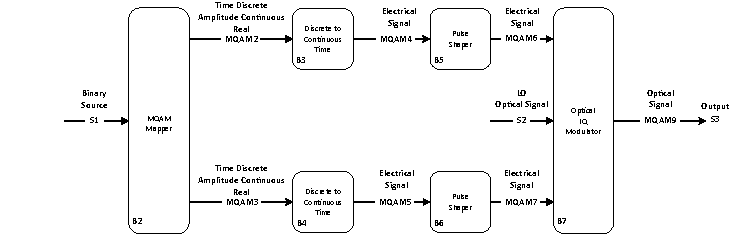
\includegraphics[width=1\textwidth]
			{./sdf/m_qam_system/figures/simulations/blockDiagrams/simulation_tx}
		\caption{Schematic representation of the MQAM Transmitter 
		block.}\label{fig:sim_txDiagram}
	\end{figure}
	\begin{figure}[]
		\centering
		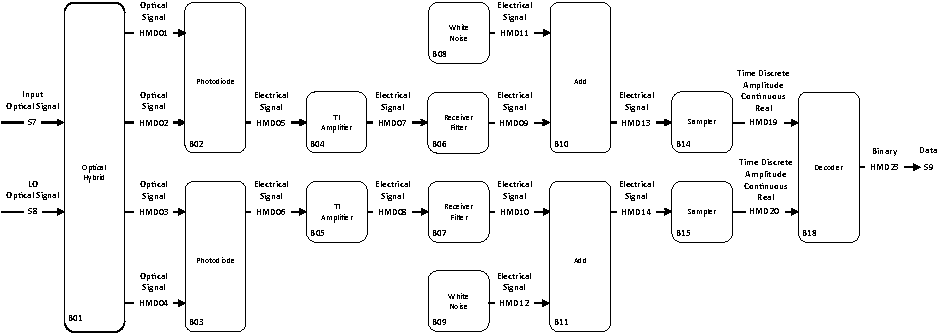
\includegraphics[width=1\textwidth]
			{./sdf/m_qam_system/figures/simulations/blockDiagrams/simulation_rx}
		\caption{Simplified schematic representation of the Homodyne Receiver 
block.}\label{fig:simulation_rx}
	\end{figure}

	\begin{figure}[]
	\centering
	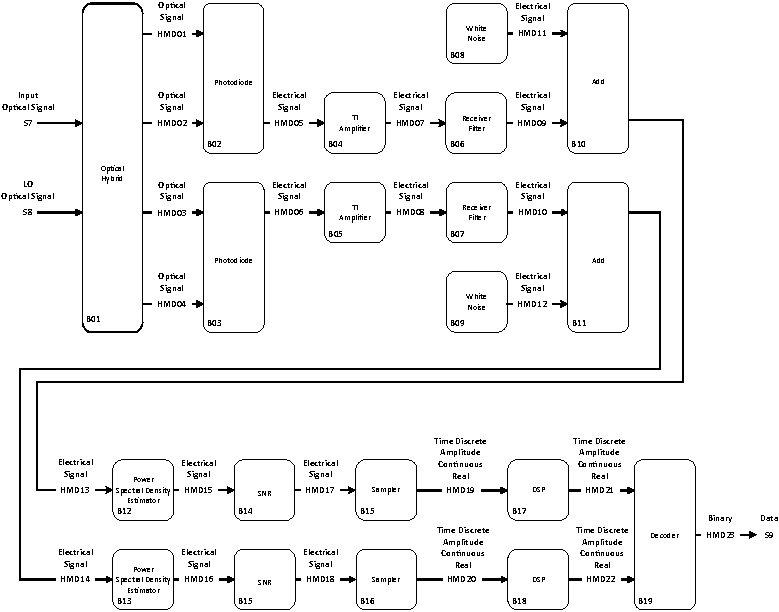
\includegraphics[width=0.9\textwidth]
	{./sdf/m_qam_system/figures/simulations/blockDiagrams/simulation_rx_wSNRAndPSD}
	\caption{Schematic representation of the Homodyne Receiver block, with the 
	DSP block (currently not implemented) and 
	two optional blocks for measuring the SNR and power spectral 
	density.}\label{fig:sim_rxDiagram}
\end{figure}


%\pagebreak
	\clearpage

	\subsubsection{Required files}\label{sec:requiredFilesMQAM}
	\begin{longtable}[h]{|l|l|l|}
		\hline
		\multicolumn{3}{|c|}{ \textbf{Source Files} } \\
		\hline
		\textbf{File}                                     & \textbf{Comments} & \textbf{Status} \\ \hline
		add\_20190215.cpp                                 &                   & 
		\checkmark \\ \hline
		binary\_source\_20190215.cpp                      &                   & 
		\checkmark \\ \hline
		bit\_error\_rate\_20190215.cpp                    &                   & 
		\checkmark \\ \hline
		decoder\_20190215.cpp                             &                   & 
		\checkmark \\ \hline
		discrete\_to\_continuous\_time\_20190215.cpp      &                   & 
		\checkmark \\ \hline
		electrical\_filter\_20190215.h                    &                   & 
		\checkmark \\ \hline
		edfa\_20190215.cpp                                          
		&                   & 
		\checkmark \\ \hline
		fft\_20180208.cpp                                 &                   & \checkmark \\ \hline
		fiber\_20190215.cpp                                         
		&                   & 
		\checkmark \\ \hline
		homodyne\_receiver\_withoutLO\_20190215.cpp                 & 
		$^{1}$            & 
		\checkmark \\ \hline
		ideal\_amplififer\_20190215.cpp                   &                   & 
		\checkmark \\ \hline
		iq\_modulator\_20190215.cpp                       &                   & 
		\checkmark \\ \hline
		local\_oscillator\_20190215.cpp                   &                   & 
		\checkmark \\ \hline
		m\_qam\_mapper\_20190215.cpp                      &                   & 
		\checkmark \\ \hline
		m\_qam\_system\_sdf.cpp                           & $^{2}$            & \checkmark \\ \hline
		m\_qam\_transmitter\_20190215.cpp                 &                   & 
		\checkmark \\ \hline
		netxpto\_20190215.cpp                             & $^{2}$            & 
		\checkmark \\ \hline
		optical\_hybrid\_20190215.cpp                     &                   & 
		\checkmark \\ \hline
		photodiode\_old\_20190215.cpp                     &                   & 
		\checkmark \\ \hline
		power\_spectral\_density\_estimator\_20190215.cpp &                   & 
		\checkmark \\\hline
		pulse\_shaper\_20190215.cpp                       &                   & 
		\checkmark \\ \hline
		sampler\_20190215.cpp                             &                   & 
		\checkmark \\ \hline
		sink\_20190215.cpp                                &                   & 
		\checkmark \\ \hline
		snr\_estimator\_20190215.cpp                      &                   & 
		\checkmark \\\hline
		super\_block\_interface\_20190215.cpp             & $^{2}$            & 
		\checkmark \\ \hline
		white\_noise\_20190215.cpp                        &                   & 
		\checkmark \\ \hline
		window\_20180704.cpp                              &                   & 
		\checkmark \\\hline
		\caption{$^1$ The library entry is under a different name, \textit{m\_qam\_receiver};\\
			$^2$ No library entry as it is a main or general purpose file, not a
		specific block.\label{tab:sources}}\\
	\end{longtable}

	\begin{longtable}[h]{|l|l|l|}
		\hline
		\multicolumn{3}{|c|}{ \textbf{Header Files} } \\
		\hline
		\textbf{File}                                   & \textbf{Comments} & \textbf{Status} \\ \hline
		add\_20190215.h                                 &                   & 
		\checkmark \\ \hline
		binary\_source\_20190215.h                     &                   & 
		\checkmark \\ \hline
		bit\_error\_rate\_20190215.h                    &                   & 
		\checkmark \\ \hline
		decoder\_20190215.h                             &                   & 
		\checkmark \\ \hline
		discrete\_to\_continuous\_time\_20190215.h      &                   & 
		\checkmark \\ \hline
		electrical\_filter\_20190215.h                  &                   & 
		\checkmark \\\hline
		edfa\_20190215.h                                          
		&                   & 
		\checkmark \\ \hline
		fft\_20180208.h                                 &                   & \checkmark \\\hline
		fiber\_20190215.h                                         
		&                   & 
		\checkmark \\ \hline
		homodyne\_receiver\_withoutLO\_20190215.h                 & 
		$^{1}$            & 
		\checkmark \\ \hline
		ideal\_amplifier\_20190215.h                    &                   & 
		\checkmark \\ \hline
		iq\_modulator\_20190215.h                       &                   & 
		\checkmark \\ \hline
		local\_oscillator\_20190215.h                   &                   & 
		\checkmark \\ \hline
		m\_qam\_mapper\_20190215.h                      &                   & 
		\checkmark \\ \hline
		m\_qam\_transmitter\_20190215.h                 &                   & 
		\checkmark \\ \hline
		netxpto\_20190215.h                             & $^2$              & 
		\checkmark \\ \hline
		optical\_hybrid\_20190215.h                     &                   & 
		\checkmark \\ \hline
		photodiode\_old\_20190215.h                     &                   & 
		\checkmark \\ \hline
		power\_spectral\_density\_estimator\_20190215.h &                   & 
		\checkmark \\\hline
		pulse\_shaper\_20190215.h                       &                   & 
		\checkmark \\ \hline
		sampler\_20190215.h                             &                   & 
		\checkmark \\ \hline
		sink\_20190215.h                                &                   & 
		\checkmark \\ \hline
		snr\_estimator\_20190215.h                      &                   & 
		\checkmark \\\hline
		super\_block\_interface\_20190215.h             & $^2$              & 
		\checkmark \\ \hline
		white\_noise\_20190215.h                        &                   & 
		\checkmark \\ \hline
		window\_20180704.h                              &                   & 
		\checkmark \\\hline
		\caption{$^1$ The library entry is under a different name, \textit{m\_qam\_receiver}\\
			$^2$ No library entry as it is a main or general purpose file, not a
		specific block. \label{tab:headers}}\\
	\end{longtable}

	\subsubsection{Input Parameters}\label{sec:inputParamsMQAM}

	\begin{longtable}[h]{|c|c|p{5cm}|}
		\caption{Input parameters}\label{table:in_par}\\\hline

		\textbf{Parameter} & \textbf{Type} & \textbf{Description}     \\ \hline

		numberOfBitsGenerated         & t\_integer
																	& Determines the number of bits to be generated by the
																	binary source\\ \hline
		samplingRate                  & double
																	& The simulation sampling rate \\\hline
		symbolRate                    & double
																	& The symbol rate of the main signal \\\hline
		samplesPerSymbol              & t\_integer
																	& Number of samples per symbol. Defined from
																	the samplingRate and symbolRate.    \\ \hline
		symbolPeriod                  & double
																	& Period of the main signal \\\hline
		bitPeriod                     & double
																	& Periodicity of bits in the main signal \\\hline
		prbsPatternLength             & int
																	& Determines the length of the pseudorandom
																	sequence Pattern (used only when the binary
																	source is operated in \textit{PseudoRandom}
																	mode)     \\ \hline
		bitPeriod                     & t\_real
																	& Temporal interval occupied by one bit     \\ \hline
		rollOffFactor\_shp            & t\_real
																	& Roll-off factor of the pulse shaper filter     \\ \hline
		rollOffFactor\_out            & t\_real
																	& Roll-off factor of the output filter     \\ \hline
		shaperFilter                  & enum
																	& Type of filter used in Pulse Shaper     \\ \hline
		outputFilter                  & enum
																	& Type of filter used in output filter     \\ \hline
		seedType                      & enum
																	& Method of seeding noise generators     \\ \hline
		seedArray                     & array<int,2>
																	& Seeds to initialize noise generators     \\ \hline
		signalOutputPower\_dBm        & t\_real
																	& Determines the power of the output optical
																	signal in dBm   \\ \hline
		numberOfBitsReceived          & int
																	&   Determines when the simulation should
																	stop. If $-1$ then it only stops when there is
																	no more bits to be sent   \\ \hline
		symbolPeriod                  & double
																	& Calculated from symbolRate     \\ \hline
		fiberLength\_m                 & t\_real & Optical fiber length \\\hline
		attentuationCoefficient       & t\_real & Optical fiber attenuation 
		coefficient 
		 \\\hline
		dispersionCoefficient         & t\_real & Optical fiber dispersion 
		coefficient \\\hline
		opticalGain\_dB               & t\_real & Optical gain of the EDFA \\\hline
		noiseFigure                   & t\_real & Noise figure of the EDFA \\\hline
		localOscillatorPower\_dBm     & t\_real
																	& Power of the local oscillator     \\ \hline
		localOscillatorPhase          & t\_real
																	& Phase of the local Oscillator \\\hline
		responsivity                  & t\_real
																	& Responsivity of the photodiodes (1
																	corresponds to having all optical power
																	transformed into electrical current)     \\
																	\hline
		amplification                 & t\_real
																	& Amplification provided by the ideal amplifier     \\ \hline
		thermalNoiseSpectralDensity   & t\_real
																	& Noise spectral density added after the electrical filter \\\hline
		amplifierNoiseSpectralDensity & t\_real
																	& Electrical noise spectral density added before the
																	electrical filter \\\hline
		elFilterType                  & enum
																	& Type of the electrical filter: generated low
																	pass or defined by coefficients \\\hline
		elFilterOrder                 & enum
																	& Order of the electrical filter \\\hline
		impulseResponseArr            & t\_real[]
																	& Array of coefficients of the electrical
																	filter. \\\hline
		iqAmplitudeValues             & vector<t\_iqValues>
																	& Determines the constellation used to encode
																	the signal in IQ space \\\hline
		samplesToSkip                 & t\_integer
																	& Number of samples to be skipped by the
																	\textit{sampler} block     \\ \hline
		confidence                    & t\_real
																	& Determines the confidence limits for the BER
																	estimation     \\ \hline
		midReportSize                 & t\_integer
																	&      \\ \hline
		bitSourceMode                 & enum
																	& Mode of generating the bitstream for the
																	signal	\\\hline
		electricalSNRMethod           & enum
																	& Mode for calculating the SNR prior to the
																	matched filter	\\\hline
		filteredSNRMethod             & enum
																	& Mode for calculating the SNR after the
																	matched filter	\\\hline
		SNRignoreSamples              & int
																	& Number of samples to initially ignore when
																	calculating the SNR \\\hline
		SNRsegmentSize                & int
																	& Size of each segment used for estimating the
																	SNR \\\hline
		powerSpectralDensityOverlap   & double
																	& Percentage of the signal to overlap when
																	averaging periodograms in power spectral
																	density estimation \\\hline
		powerSpectralDensitySegment   & int
																	& Size of segment used for calculating each
																	periodogram \\\hline
		powerSpectralDensityInterval  & int
																	& Number of samples to acquire before
																	estimating the power spectral density \\\hline
		bufferLength                  & t\_integer
																	& Corresponds to the number of samples that
																	can be processed in each run of the system
																	\\ \hline
	\end{longtable}

	\subsubsection{Output Files}\label{sec:outputFilesMQAM}

	\begin{longtable}[h]{|c|p{5cm}|}
		\caption{Output Files}\label{table:out_files}\\\hline

		\textbf{Files} & \textbf{Description}     \\ \hline
		\textit{Signal.sgn}				& Files with corresponding signal data generated
			in the simulation. \\\hline
		BER.txt                   & Results from bit\_error\_rate block. \\ \hline
		log.txt                   & Log file from simulation. \\ \hline
		params.txt                & Input parameter list. \\ \hline
		PowerSpectralDensity.txt  & Power spectral density estimate from optical
			signal. \\ \hline
		PowerSpectralDensity2.txt & Power spectral density estimate from electrical
			signal. \\ \hline
		SNR.txt                   & SNR estimate before matched filter. \\ \hline
		SNRFiltered.txt           & SNR estimate after matched filter.	\\ \hline
		impulse\_response.imp     & Impulse response from electrical filter. \\ \hline
		out\_filter.imp           & Impulse response from matched filter. \\ \hline
		pulse\_shaper.imp         & Pulse shaper impulse response. \\ \hline
	\end{longtable}

\subsubsection{Simulation results - ISI}\label{sec:simRes_ISI}

	In this section we will explore the signals generated during the simulation.
	The general scheme of the simulation is shown in
	Figures~\ref{fig:sim_systemDiagram}, ~\ref{fig:sim_txDiagram}
	and~\ref{fig:sim_rxDiagram}. Every signal generated during the simulation 
	is
	identified in those diagrams.
	
	We will start by analyzing the intersymbol interference (ISI) in the signals 
	generated on the simulation. For this purpose, we will turn of all noise 
	sources. We will be using 
	root-raised cosines at the pulse shaper (\textit{B5} and \textit{B6} on MQAM 
	transmitter) and 
	at the matched filter (\textit{B18} and \textit{B19} at the homodyne 
	receiver). With this 
	configuration, we should obtain a perfect copy of the transmitted 
	constellation, affected only by a scaling factor (which could be removed by 
	adjusting the \textit{amplification} parameter).

	The parameters used to obtain the plots and eye diagrams
	in this section are displayed in Table~\ref{tab:noNoiseSimParams}.

	\begin{longtable}[h]{|l|l|l|}
		\caption{Simulation parameters\label{tab:noNoiseSimParams}}\\\hline
		\textbf{Parameter}            & \textbf{Value}       &\textbf{Units}\\\hline
		numberOfBitsGenerated         & $100 \times 10^3$    & \\\hline
		samplingRate                  & $64 \times 10^9$     & Hz \\\hline
		symbolRate                    & $4 \times 10^9$      & Bd \\\hline
		samplesPerSymbol              & 16                   & \\\hline
		symbolPeriod                  & $250\times 10^{-12}$ & s\\\hline
		bitPeriod                     & $125\times 10^{-12}$ & s\\\hline
		signalOutputPower\_dBm        & -10                  & dBm\\\hline
		localOscillatorPower\_dBm     & 0                    & dBm\\\hline
		localOscillatorPhase          & 0                    & rad\\\hline
		nBw                           & $18\times10^9$       & Hz\\\hline
		amplification                 & 3162.28              & \\\hline
		responsivity                  & 1                    & A/W\\\hline
		outputFilter                  & RootRaisedCosine     & \\\hline
		shaperFilter                  & RootRaisedCosine     & \\\hline
		rollOffFactor\_out            & 0.9                  & \\\hline
		rollOffFactor\_shp            & 0.9                  & \\\hline
		seedType                      & RandomDevice         & \\\hline
		numberOfBitsReceived          & -1                   & \\\hline
		elFilterType                  & Defined              & \\\hline
		elFilterOrder                 & 20                   & \\\hline
		opticalGain\_dB               & 0                    & dB \\\hline
		noiseFigure                   & 0                    & dB \\\hline
		preFilterNoiseSpectralDensity & 0                    & W/Hz\\\hline
		elNoiseSpectralDensity        & 0                    & W/Hz\\\hline
		bufferLength                  & 512                  & \\\hline
		bitSourceMode                 & Random               & \\\hline
		confidence                    & 0.95                 & \\\hline
	\end{longtable}


	We will start by showing the signals present in the 
	\textit{m\_qam\_transmitter} block, shown
	in Figure~\ref{fig:sim_txDiagram}. This is the block where the signals are 
	generated and modulated, and remains unaltered for all cases shown here. 
	Therefore, to avoid repetition, these signals will only be shown here, as 
	their properties remain similar for all the other simulation that will be 
	examined further on.

	First, the initial bitstream is generated. This is the pseudorandom array of 
	ones and zeros which will be transmitted, and later compared with the decoded 
	signal.
	
	% Initial bitstream
	\begin{figure}[H]
			\centering
\begin{minipage}{0.45\textwidth}
	\centering
	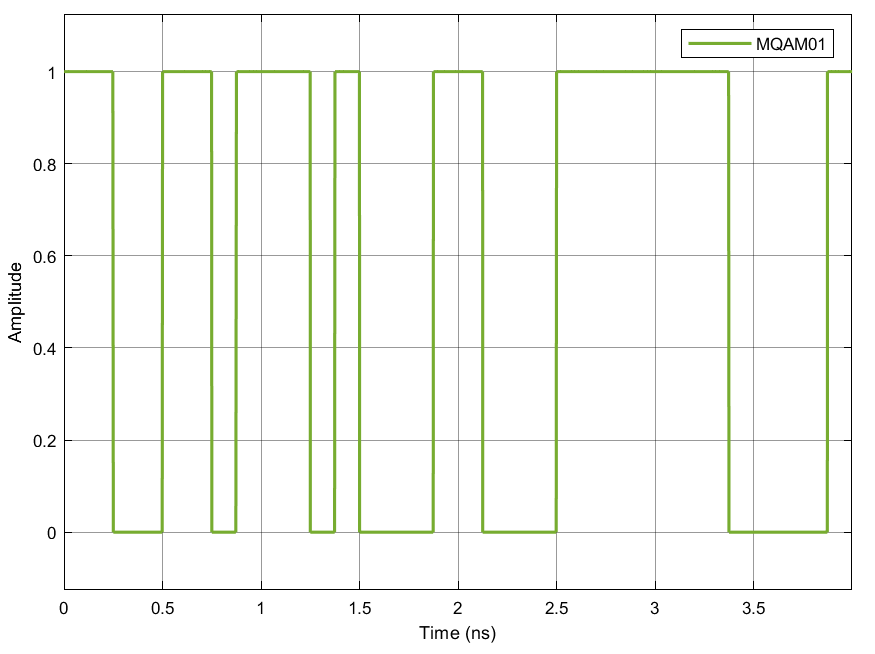
\includegraphics[width=1\textwidth]
	{./sdf/m_qam_system/figures/simulations/01_noISI/MQAM01.pdf}
	\subcaption{}
\end{minipage}
\begin{minipage}{0.4\textwidth}
	\centering
	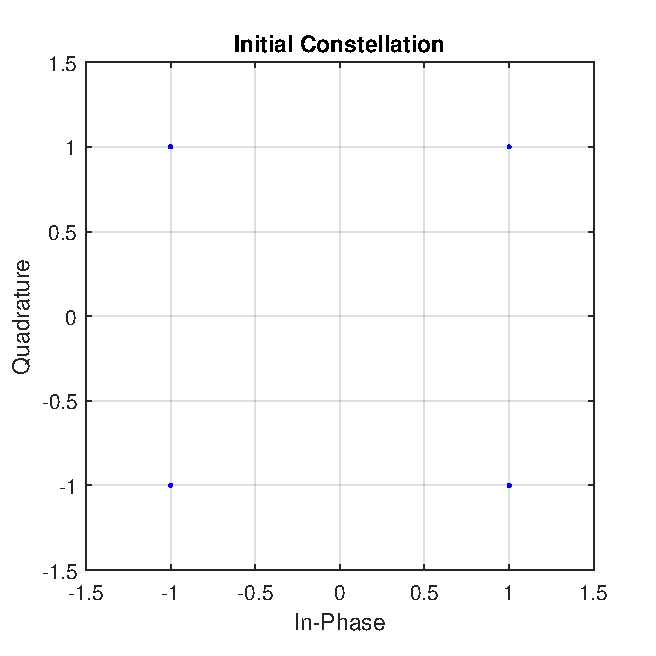
\includegraphics[width=\textwidth]
	{./sdf/m_qam_system/figures/simulations/01_noISI/constStart.pdf}
	\subcaption{}
\end{minipage}
			%			\includegraphics[width=1\textwidth]
			%			{./sdf/m_qam_system/figures/eyes/noNoise/MQAM5.pdf}
			\caption{Eye diagram of initial bitstream MQAM01 (pseudorandom ones and 
			zeros), and respective constellation to be used.}
	\end{figure}

This series of bits needs to be encoded into the corresponding coordinate 
points, according to the chosen constellation and modulation format. As we are 
using a 4 point QAM modulation, these coordinate points are (1,1), (1,-1), 
(-1,-1) and (-1,1). Mapping the bits to these points is done in the 
\textit{MQAM\_mapper} block. This block receives the binary sequence and 
outputs two signals, discrete in time and value. Each bit is alternately coded 
into one of the output signals, according to the chosen constellation. In this 
case, the values are either 1 or -1.
Each signal contains the values ultimately used to modulate either 
the in-phase or quadrature component.

	\begin{figure}[H]
		\centering
		\begin{minipage}{0.45\textwidth}
			\centering
			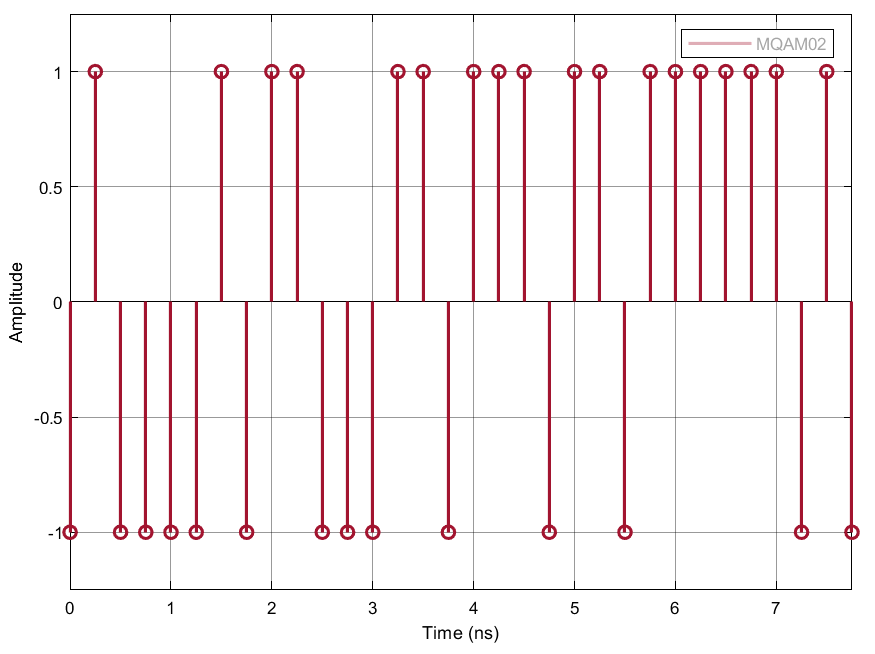
\includegraphics[width=1\textwidth]		
			{./sdf/m_qam_system/figures/simulations/01_noISI/MQAM02.pdf}
			\subcaption{}\label{fig:ISImqam2}
		\end{minipage}
		\begin{minipage}{0.45\textwidth}
			\centering
			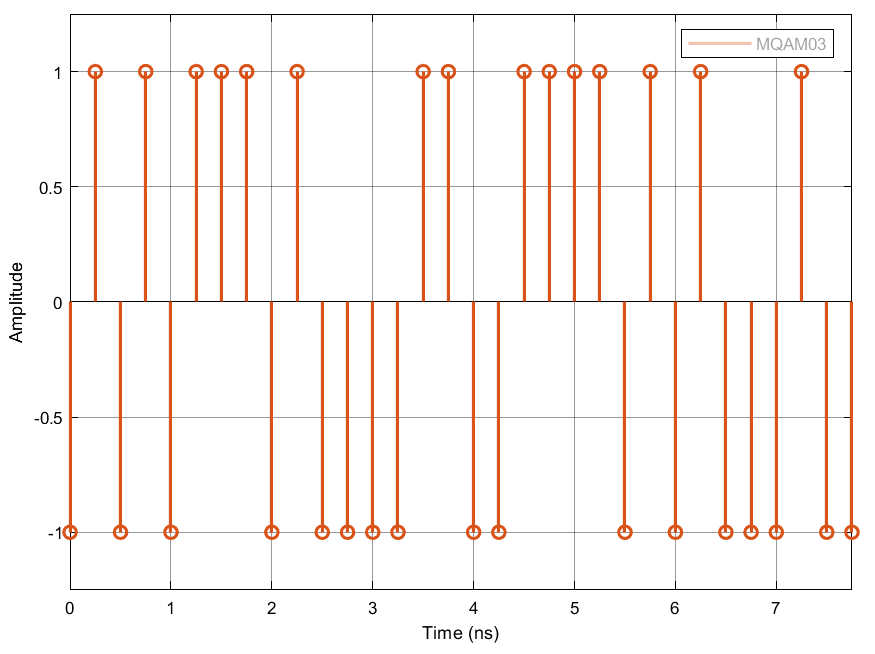
\includegraphics[width=1\textwidth]
			{sdf/m_qam_system/figures/simulations/01_noISI/MQAM03.pdf}
			\subcaption{}\label{fig:ISImqam3}
		\end{minipage}
		\caption{Signals MQAM02~(\subref{fig:ISImqam2}) and 
		MQAM03~(\subref{fig:ISImqam3}), 
		containing the values encoded and distributed to the in-phase and quadrature
		components.}
	\end{figure}

As mentioned before, the signals MQAM02 and MQAM03 are discrete in both value 
and 
time. However, in order to be used for modulating the optical signal, they need 
to 
be continuous in time. Also, they have to be assigned a given continuous 
shape that can be modulated onto the optical signal.

The first of these requirements is fixed with the 
\textit{discrete\_to\_continuous\_time} block. This block takes the discrete 
sequence of values generated on the previous block and outputs an equivalent 
where each value (or symbol) has a proper timing. Therefore, it outputs the 
previous sequence of values, but in an array continuous in time, with each 
value separated by an amount of time 
equal to the desired symbol period.

	\begin{figure}[H]
	\centering
	\begin{minipage}{0.45\textwidth}
		\centering
		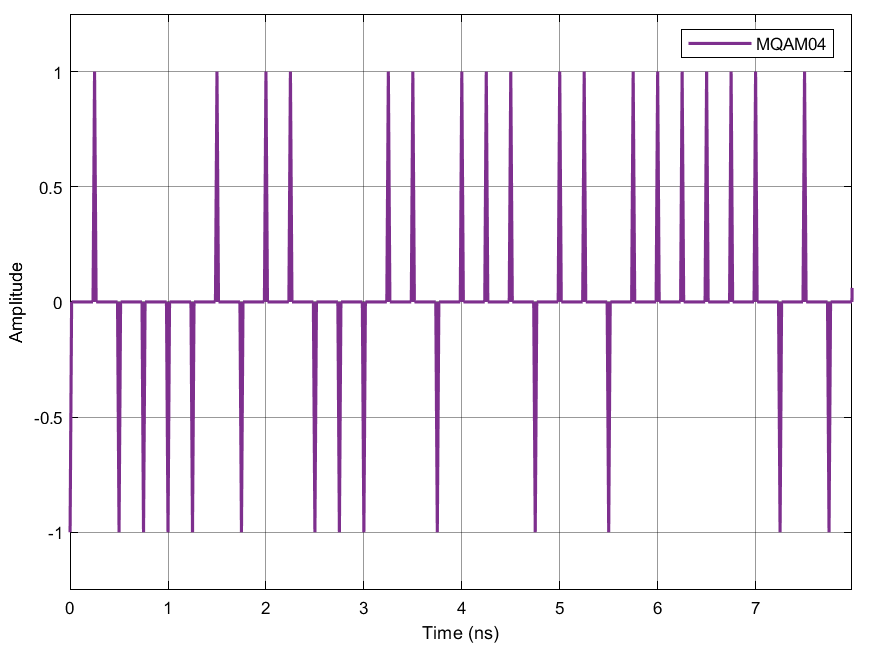
\includegraphics[width=1\textwidth]		
		{./sdf/m_qam_system/figures/simulations/01_noISI/MQAM04.pdf}
		\subcaption{}\label{fig:ISImqam4}
	\end{minipage}
	\begin{minipage}{0.45\textwidth}
		\centering
		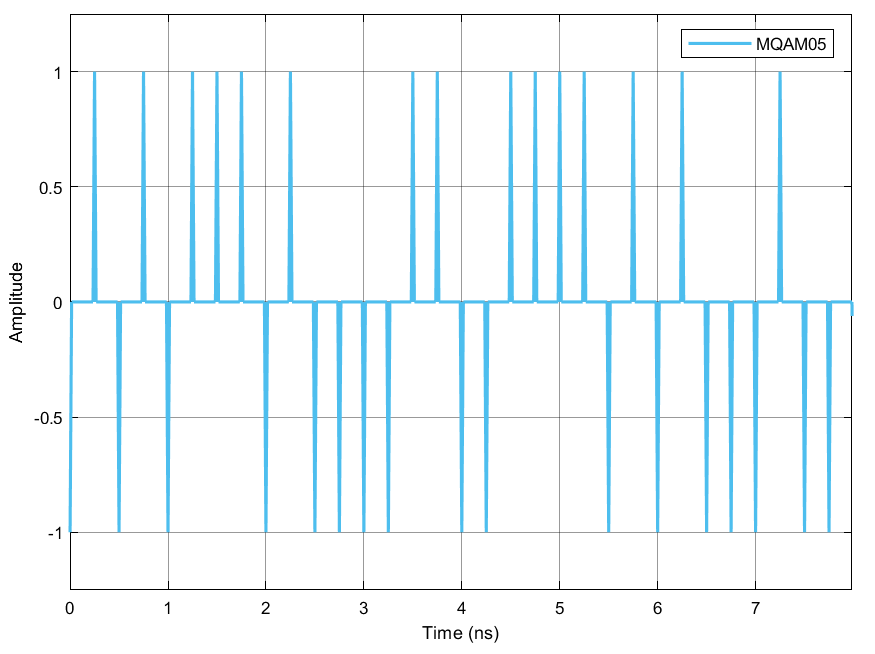
\includegraphics[width=1\textwidth]
		{sdf/m_qam_system/figures/simulations/01_noISI/MQAM05.pdf}
		\subcaption{}\label{fig:ISImqam5}
	\end{minipage}
	\caption{Signals MQAM04~(\subref{fig:ISImqam4}) and 
	MQAM05~(\subref{fig:ISImqam5}), 
		containing the values in a signal with continuous time.}
\end{figure}

	The signals still need to be assigned a continuous shape in order to modulate 
	them into the optical signal. This is done with a pulse shaper, which acts as 
	a 
	FIR filter shaping the discretely-valued sequences of symbols. As mentioned 
	in the beginning of the section, the chosen filter is a root-raised-cosine.

	\begin{figure}[H]
	\centering
	\begin{minipage}{0.45\textwidth}
		\centering
		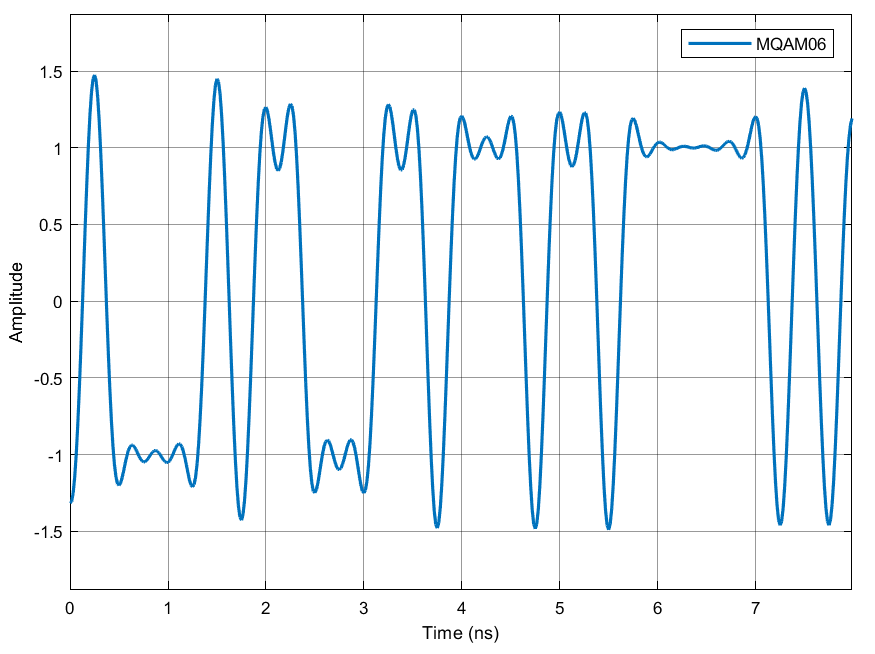
\includegraphics[width=1\textwidth]		
		{./sdf/m_qam_system/figures/simulations/01_noISI/MQAM06.pdf}
		\subcaption{}\label{fig:ISImqam6}
	\end{minipage}
	\begin{minipage}{0.45\textwidth}
		\centering
		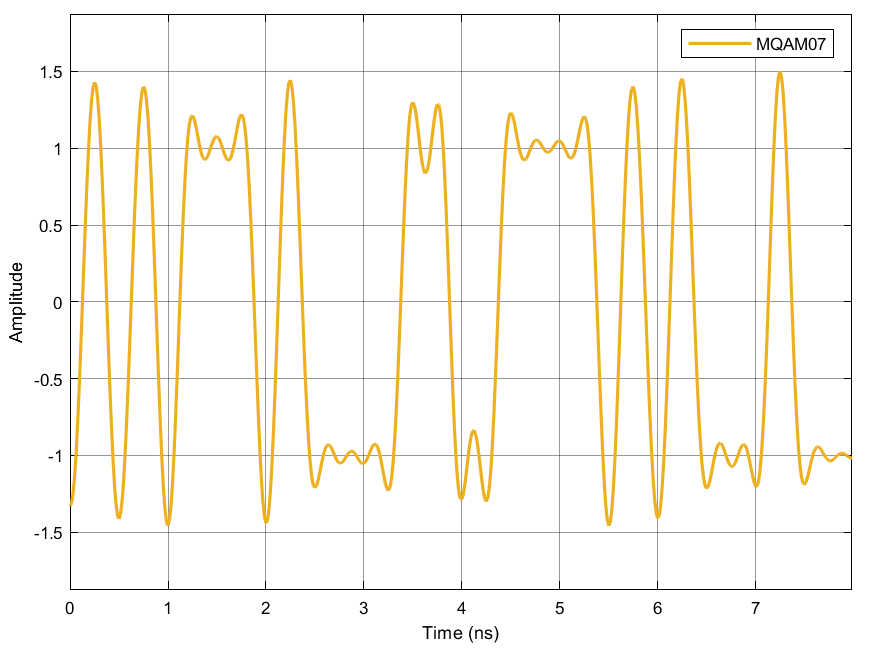
\includegraphics[width=1\textwidth]
		{sdf/m_qam_system/figures/simulations/01_noISI/MQAM07.pdf}
		\subcaption{}\label{fig:ISImqam7}
	\end{minipage}
	\caption{Signals MQAM06~(\subref{fig:ISImqam6}) and 
	MQAM07~(\subref{fig:ISImqam7}), 
		containing the signals to be modulated, already shaped with a 
		root-raised-cosine filter.}
\end{figure}

	\begin{figure}[H]
	\centering
	\begin{minipage}{0.45\textwidth}
		\centering
		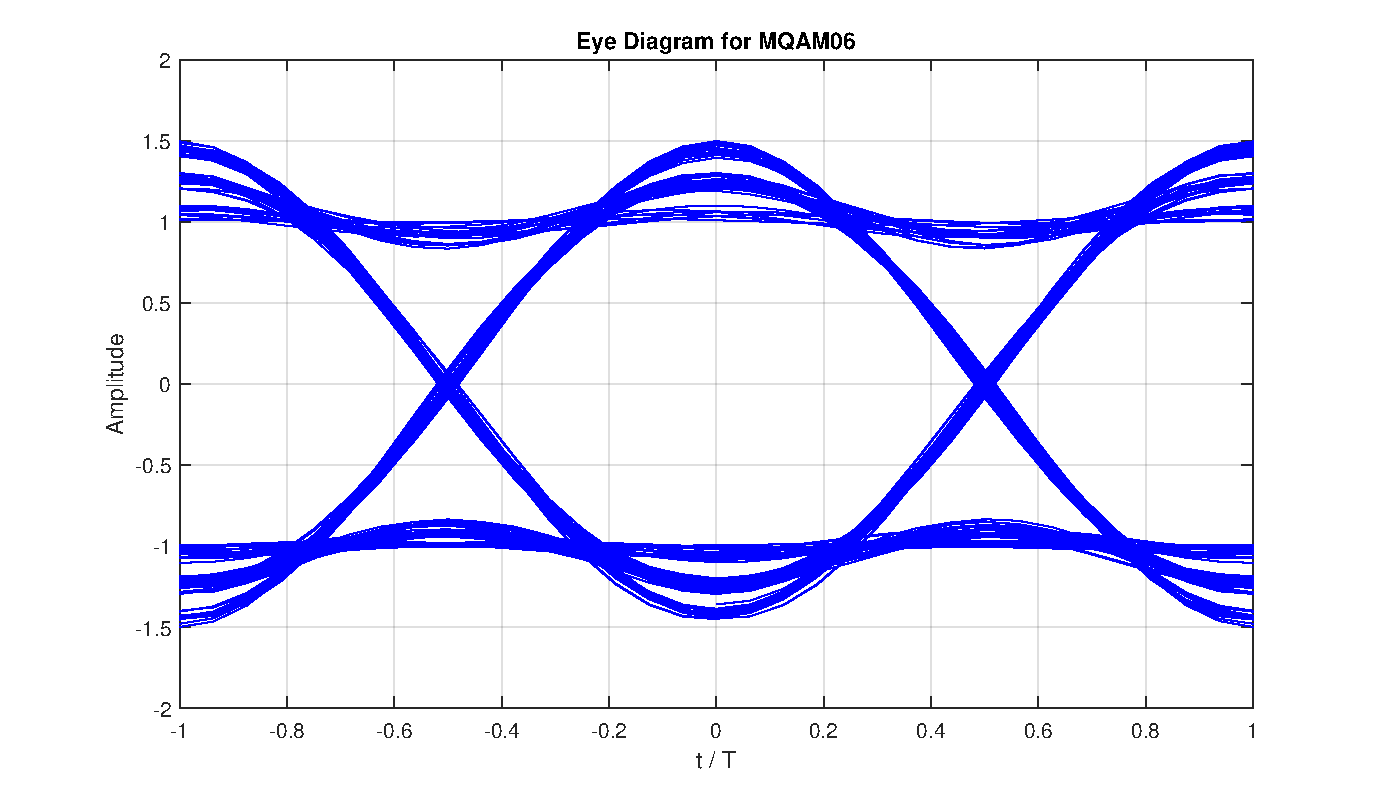
\includegraphics[width=1\textwidth]		
		{./sdf/m_qam_system/figures/simulations/01_noISI/MQAM06_edl.pdf}
		\subcaption{}\label{fig:ISImqam6ed}
	\end{minipage}
	\begin{minipage}{0.45\textwidth}
		\centering
		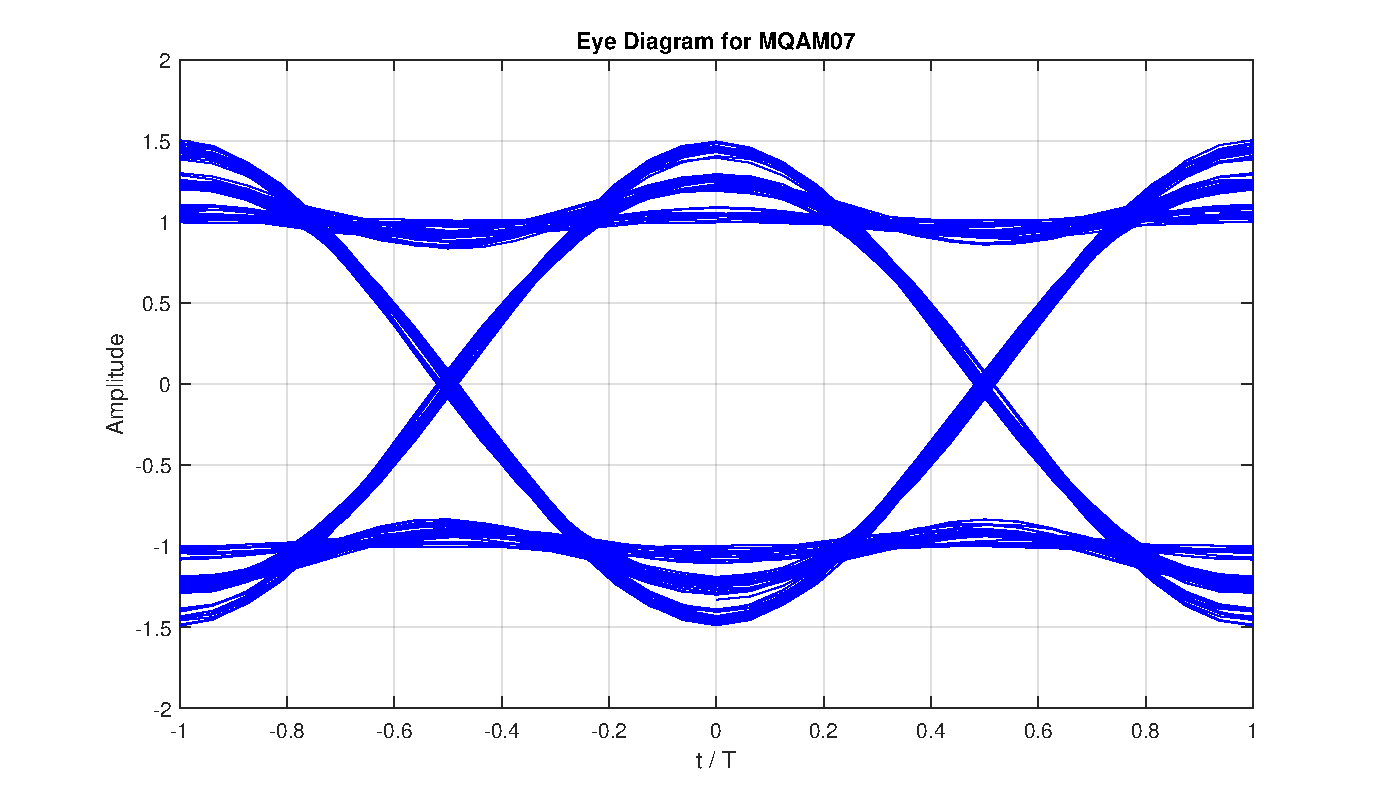
\includegraphics[width=1\textwidth]
		{sdf/m_qam_system/figures/simulations/01_noISI/MQAM07_edl.pdf}
		\subcaption{}\label{fig:ISImqam7ed}
	\end{minipage}
	\caption{Eye diagrams for MQAM06~(\subref{fig:ISImqam6ed}) and 
		MQAM07~(\subref{fig:ISImqam7ed}), shaped with root-raised-cosines.}
\end{figure}

	It can be seen in the eye diagrams that the signal is not free from ISI. 
	However, as mentioned in section~\ref{sec:ISI}, the shaping is done at the 
	transmitter and at the receiver. We shall see further ahead that the signal 
	will be free of ISI at sampling time.

	Being continuous in time and in value, signals MQAM06 and MQAM07 are then 
	ready to be passed on to the 
	\textit{iq\_modulator} block, where they are modulated into an optical 
	signal, and then transmitted.

	\begin{figure}[H]
	\centering
		\centering
		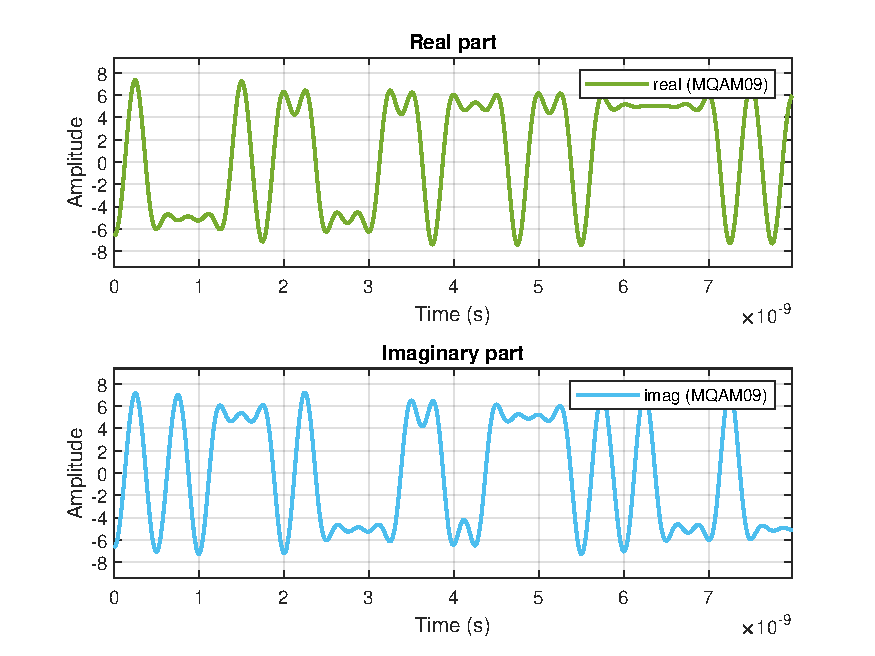
\includegraphics[width=0.7\textwidth]		
		{./sdf/m_qam_system/figures/simulations/01_noISI/MQAM09.pdf}
	\caption{Signal MQAM09, modulated optical signal.}\label{fig:ISImqam9}
\end{figure}

	MQAM01 and MQAM09 are the output signals of the \textit{m\_qam\_transmitter} 
	block. They are equal to the top level signals S0 and S1, respectively.
	Normally the S1 signal is now directed to an \textit{optical\_fiber} block, 
	which is then connected to an \textit{edfa} block. However, in this 
	simulation they are both configured to have no effect, and so we shall not 
	show them here. The optical signal then proceeds to be used as input to the 
	\textit{homodyne\_receiver\_withoutLO} block, along with S4, an optical 
	signal acting as local oscillator.
	
	We shall now explore the process inside the 
	\textit{homodyne\_receiver\_withoutLO} 
	block. The inputs of the block are mixed inside an \textit{optical\_hybrid} 
	block. These outputs are a mix of the transmitted optical signal and the 
	local oscillator, as explained in 
	section~\ref{sec:teorRX}.
	
		% After optical hybrid 1
		\begin{figure}[H]
			\centering
				\centering
				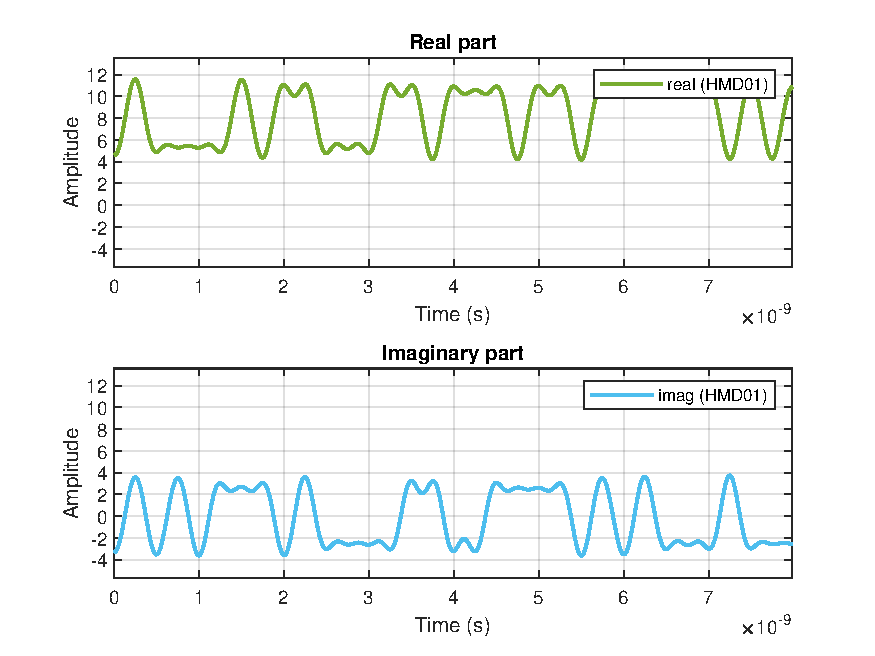
\includegraphics[width=0.7\textwidth]
				{./sdf/m_qam_system/figures/simulations/01_noISI/HMD01.pdf}
						\caption{HMD01, output 1 optical hybrid.}
		\end{figure}
	\begin{figure}[H]
				\centering
				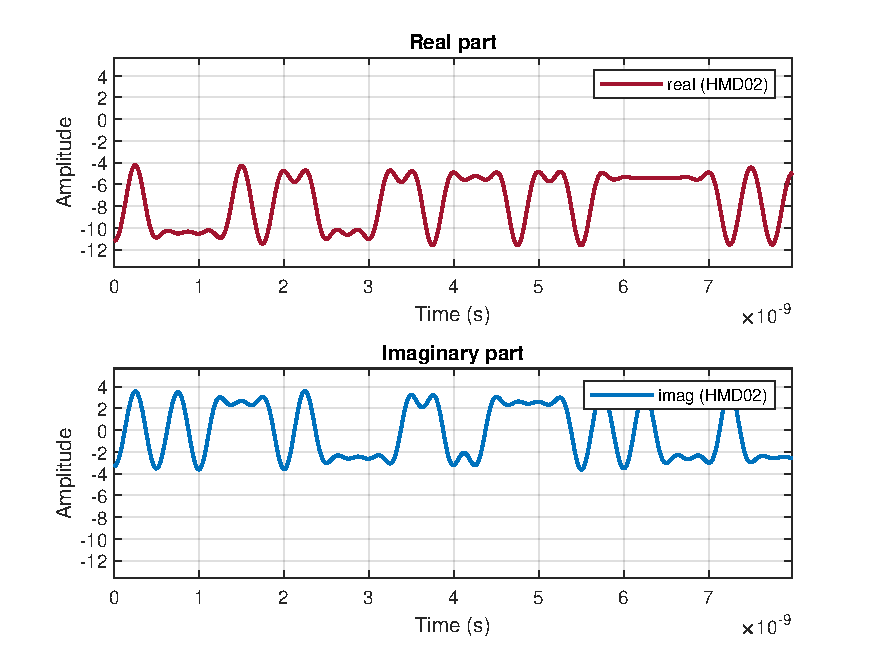
\includegraphics[width=0.7\textwidth]
				{./sdf/m_qam_system/figures/simulations/01_noISI/HMD02.pdf}
		\caption{HMD02, output 2 of the optical hybrid.}
		\end{figure}
	
		\begin{figure}[H]
			\centering
				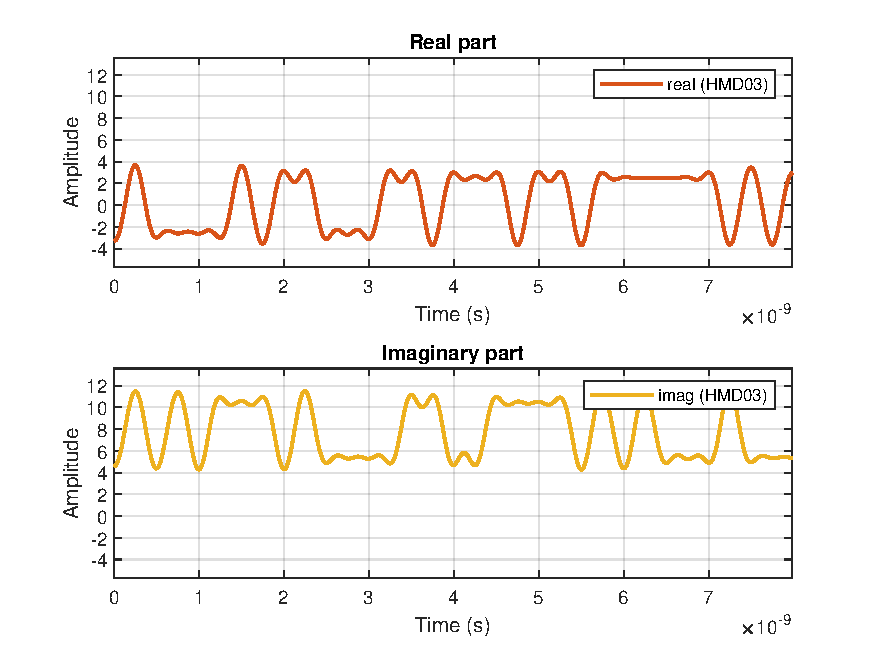
\includegraphics[width=0.7\textwidth]
				{./sdf/m_qam_system/figures/simulations/01_noISI/HMD03.pdf}
		\caption{HMD03, output 3 of the optical hybrid.}
				\end{figure}
	\begin{figure}[H]
				\centering
				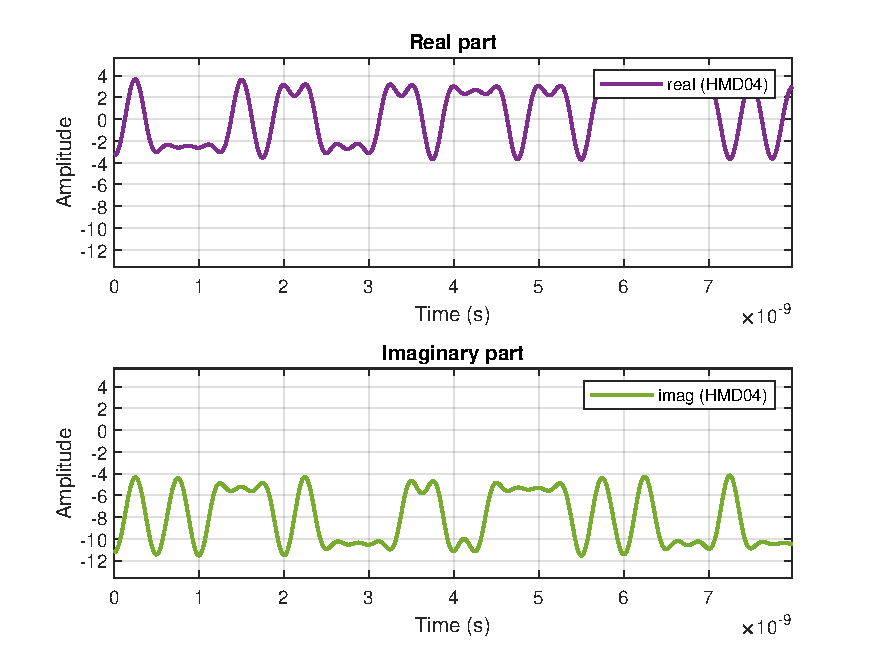
\includegraphics[width=0.7\textwidth]
				{./sdf/m_qam_system/figures/simulations/01_noISI/HMD04.pdf}
		\caption{HMD04, output 4 of the optical hybrid.}
		\end{figure}
		
	These optical signals are then sent in pairs to two \textit{photodiode} 
	blocks, where they are detected (with a \textit{responsivity} defined in the 
	parameters) and 
	subtracted. The output of the photodiode 
	blocks is then directed to the \textit{ti\_amplifier} blocks, which generate 
	the signals shown in Figure~\ref{fig:ISIhmd0708}. The \textit{ti\_amplifier} 
	usually does three things: it adds noise, amplifies the signal and noise, and 
	lastly passes the signal and noise through a filter. However, as there is no 
	noise here and the filter's bandwidth is much larger than the signal 
	bandwidth, the only visible effect is the amplification.

	\begin{figure}[H]
	\centering
	\begin{minipage}{0.45\textwidth}
		\centering
		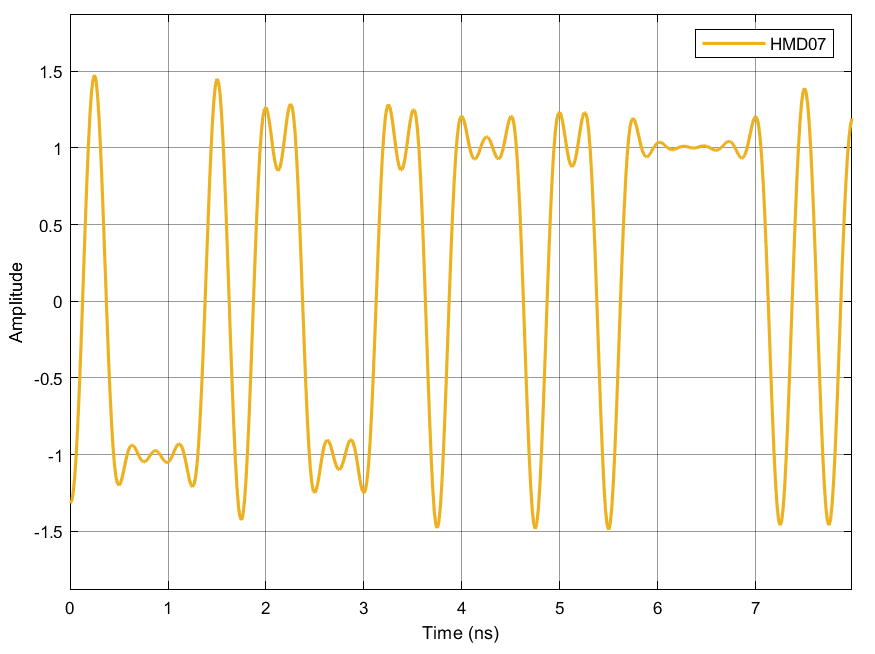
\includegraphics[width=1\textwidth]		
		{./sdf/m_qam_system/figures/simulations/01_noISI/HMD07.pdf}
		\subcaption{}\label{fig:ISIhmd07}
	\end{minipage}
	\begin{minipage}{0.45\textwidth}
		\centering
		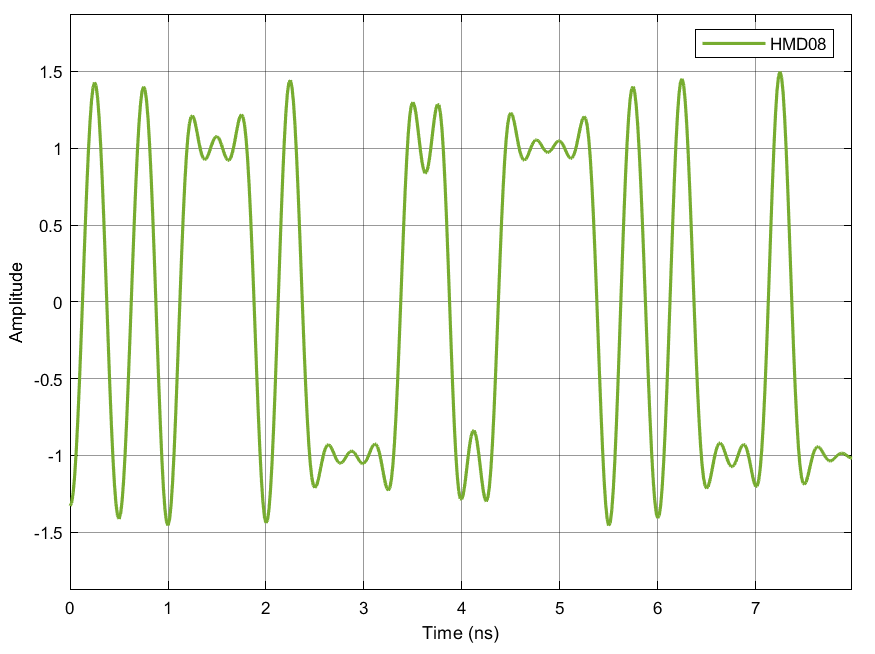
\includegraphics[width=1\textwidth]
		{sdf/m_qam_system/figures/simulations/01_noISI/HMD08.pdf}
		\subcaption{}\label{fig:ISIhmd08}
	\end{minipage}
	\caption{Signals HMD07~(\subref{fig:ISIhmd07}) and 
		HMD08~(\subref{fig:ISIhmd08}), 
		containing the amplified versions of the signals detected at the 
		\textit{photodiode} blocks}\label{fig:ISIhmd0708}
\end{figure}


The next step is the matched filter. Again, as there is no noise, the only 
visible effect is the change in the signal shape. By using another 
root-raised-cosine filter, the signal now follows a raised-cosine shape.

	\begin{figure}[H]
	\centering
	\begin{minipage}{0.45\textwidth}
		\centering
		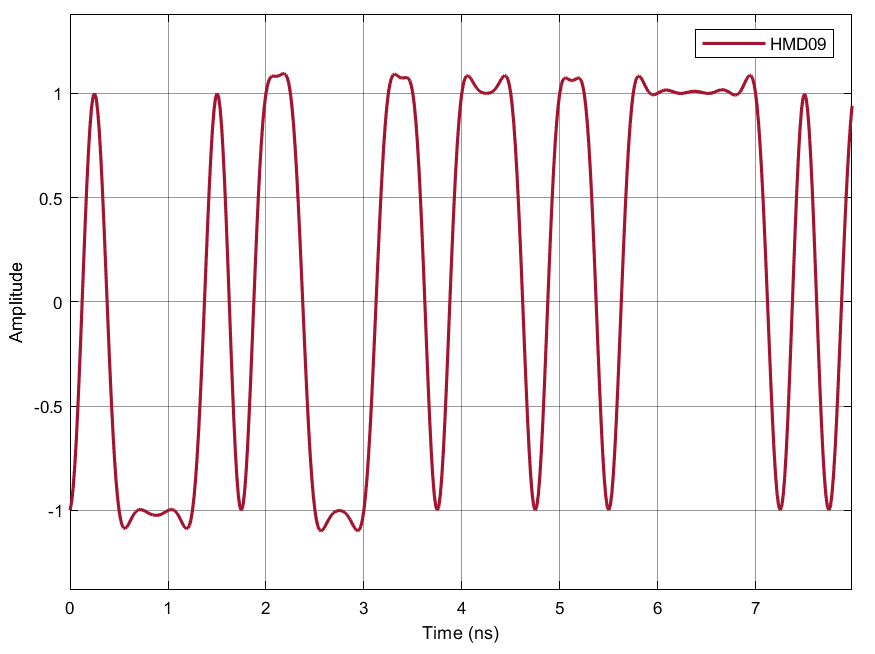
\includegraphics[width=1\textwidth]		
		{./sdf/m_qam_system/figures/simulations/01_noISI/HMD09.pdf}
		\subcaption{}\label{fig:ISIhmd09}
	\end{minipage}
	\begin{minipage}{0.45\textwidth}
		\centering
		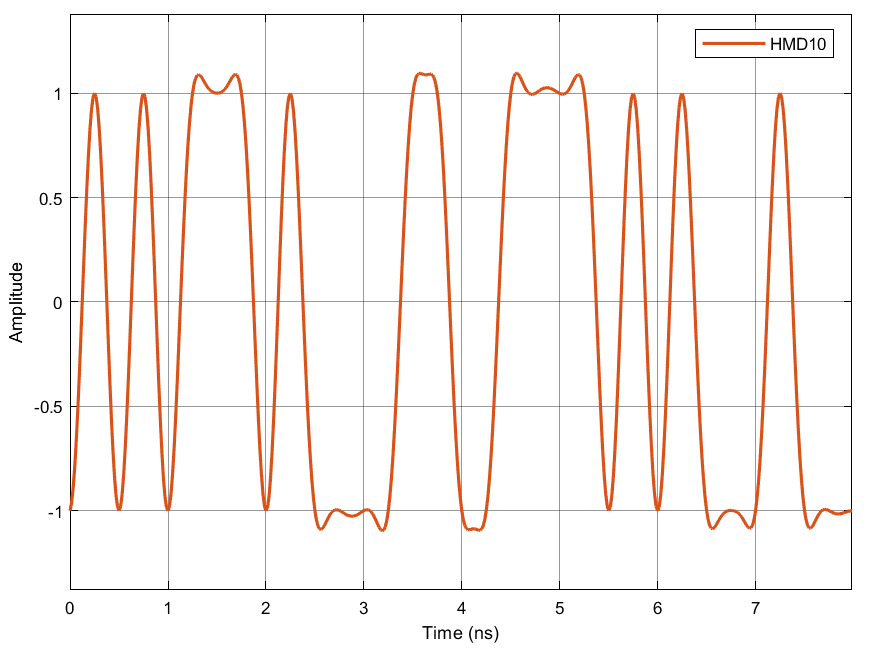
\includegraphics[width=1\textwidth]
		{sdf/m_qam_system/figures/simulations/01_noISI/HMD10.pdf}
		\subcaption{}\label{fig:ISIhmd10}
	\end{minipage}
	\caption{Signals HMD09~(\subref{fig:ISIhmd09}) and 
		HMD10~(\subref{fig:ISIhmd10}), after the root-raised-cosine matched 
		filter.}\label{fig:ISIhmd0910}
\end{figure}


	\begin{figure}[H]
	\centering
	\begin{minipage}{0.45\textwidth}
		\centering
		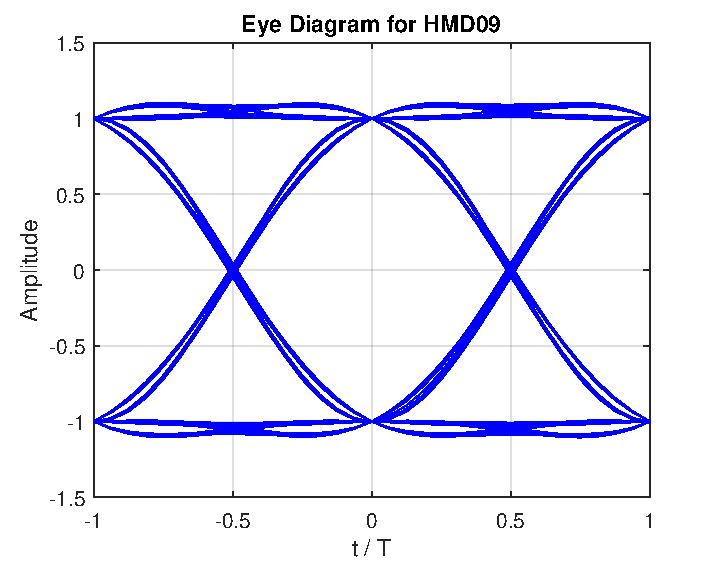
\includegraphics[width=1\textwidth]		
		{./sdf/m_qam_system/figures/simulations/01_noISI/HMD09_ed.pdf}
		\subcaption{}\label{fig:ISIhmd09ed}
	\end{minipage}
	\begin{minipage}{0.45\textwidth}
		\centering
		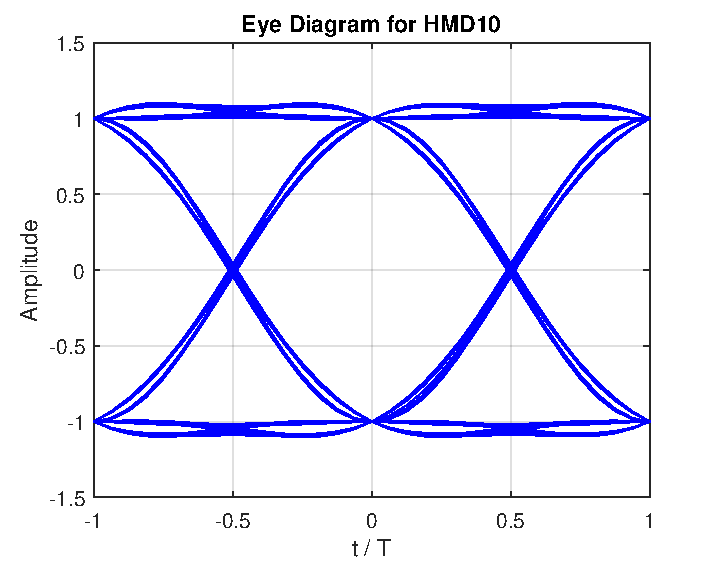
\includegraphics[width=1\textwidth]
		{sdf/m_qam_system/figures/simulations/01_noISI/HMD10_ed.pdf}
		\subcaption{}\label{fig:ISIhmd10ed}
	\end{minipage}
	\caption{Eye diagrams for HMD09~(\subref{fig:ISIhmd09ed}) and 
		HMD10~(\subref{fig:ISIhmd10ed}), after the root-raised-cosine matched 
		filter. They are now following a raised-cosine 
		shape.}\label{fig:ISIhmd0910ed}
\end{figure}

For the purpose of this simulation, no electrical noise is added at the 
receiver. So HMD09 and HMD10 are effectively the signals that will be sampled. 
As can be seen from their 
eye diagrams in Figure~\ref{fig:ISIhmd0910ed}, they suffer from no intersymbol 
interference, having always the same exact value at sampling time. This is then 
sampled and then decoded, transforming the received signal into a bitstream. As 
the reception is perfect, the received bitstream is exactly equal to the 
transmitted one.

	\begin{figure}[H]
	\centering
	\begin{minipage}{0.45\textwidth}
		\centering
		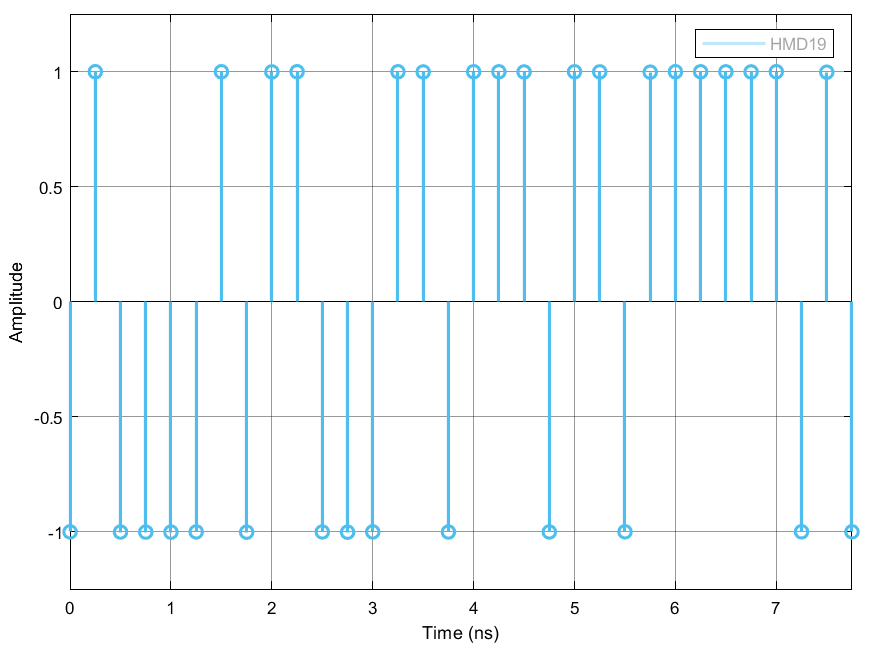
\includegraphics[width=1\textwidth]		
		{./sdf/m_qam_system/figures/simulations/01_noISI/HMD19.pdf}
		\subcaption{}\label{fig:ISIhmd19}
	\end{minipage}
	\begin{minipage}{0.45\textwidth}
		\centering
		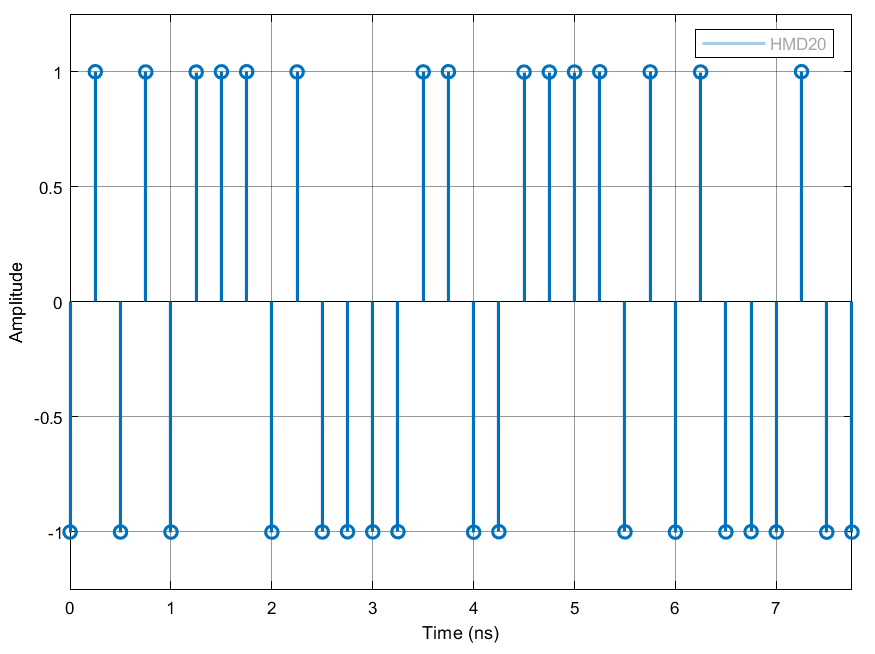
\includegraphics[width=1\textwidth]
		{sdf/m_qam_system/figures/simulations/01_noISI/HMD20.pdf}
		\subcaption{}\label{fig:ISIhmd20}
	\end{minipage}
	\caption{Signals HMD19~(\subref{fig:ISIhmd19}) and 
		HMD20~(\subref{fig:ISIhmd20}), sampled at instants 
		$t=T_s$.}\label{fig:ISIhmd1920}
\end{figure}

	\begin{figure}[H]
		\centering
		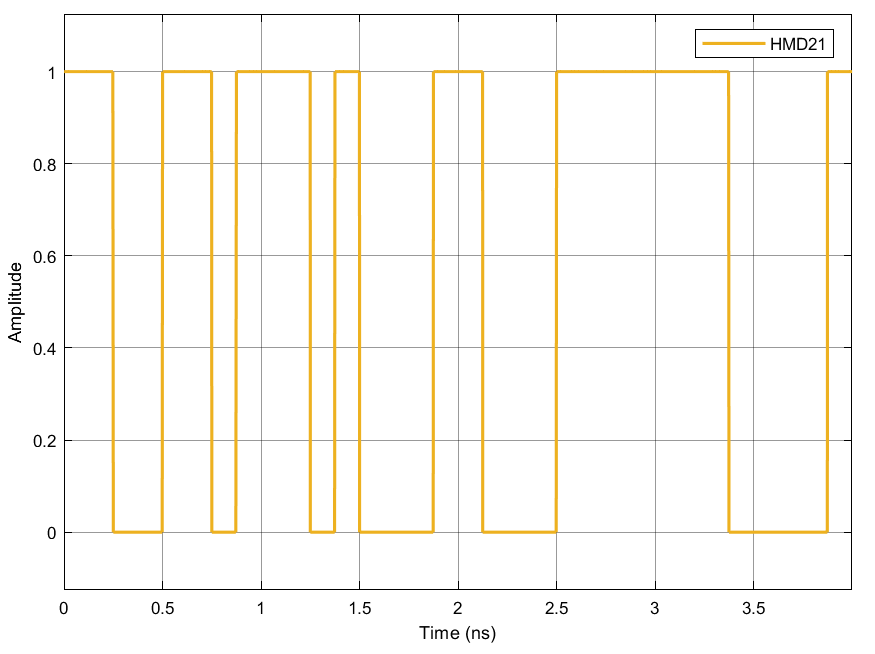
\includegraphics[width=0.5\textwidth]		
		{./sdf/m_qam_system/figures/simulations/01_noISI/HMD21.pdf}
	\caption{Signal HMD21, containing the decoded 
	bitstream.}\label{fig:ISIhmd21}
\end{figure}

	\begin{figure}[H]
		\centering
		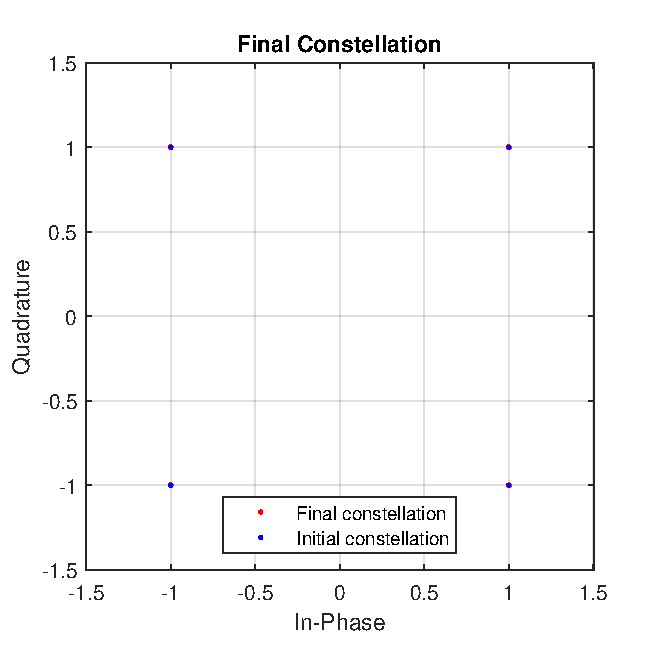
\includegraphics[width=0.7\textwidth]
		{sdf/m_qam_system/figures/simulations/01_noISI/constFinal.pdf}
	\caption{  Constellation of the encoded and decoded 
		signals. They are exactly equal due to lack of ISI and 
		noise.}\label{fig:ISIconsts}
\end{figure}

We can see that the received constellation is almost equal to the transmitted 
one, with all received 
bits having nearly no variation from their amplitude value. However, looking 
closely, we can still see a bit of the red points in 
figure~\ref{fig:ISIconsts}. This a consequence of the finite impulse response 
of the 
used filters. The ideal filters, which provide zero ISI, have infinite impulse 
response. 

\begin{figure}[H]
	\centering
	\begin{minipage}{0.3\textwidth}
		\centering
		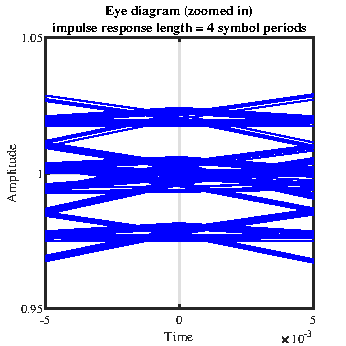
\includegraphics[width=1\textwidth]		
		{./sdf/m_qam_system/figures/simulations/01_noISI/ISI_4symbolPeriodsZoomed.pdf}
		\subcaption{}\label{fig:ISI4sp}
	\end{minipage}
	\begin{minipage}{0.3\textwidth}
		\centering
		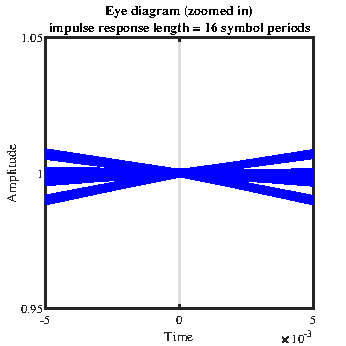
\includegraphics[width=1\textwidth]
		{sdf/m_qam_system/figures/simulations/01_noISI/ISI_16symbolPeriodsZoomed.pdf}
		\subcaption{}\label{fig:ISI16sp}
	\end{minipage}
	\begin{minipage}{0.3\textwidth}
		\centering
		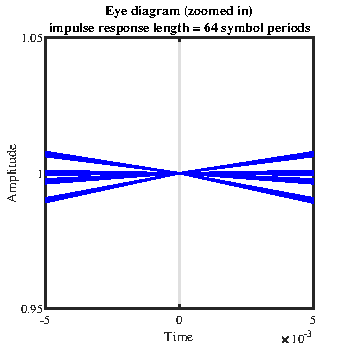
\includegraphics[width=1\textwidth]
		{sdf/m_qam_system/figures/simulations/01_noISI/ISI_64symbolPeriodsZoomed.pdf}
		\subcaption{}\label{fig:ISI64sp}
	\end{minipage}
	\caption{Zoom in on the eye diagram at sampling time. The figures used 
	filter impulse responses with lengths of (\subref{fig:ISI4sp}) 4, 
	(\subref{fig:ISI16sp})16 and 
	(\subref{fig:ISI64sp}) 64 symbol periods. As the filter impulse 
	response increases in size, the vestigial amount of ISI 
	diminishes.}\label{fig:ISIdemo}
\end{figure}

However, the practical implementation of the FIR filter implies that 
the impulse response is finite, leading to very small variations at sampling 
time. This effect can be diminished by using a larger impulse response. We have 
conducted the simulations using impulse responses with a size of 16 symbol 
periods. We can see in Figure~\ref{fig:ISI16sp} that this effect is not 
particularly significant for this situation, and thus we can consider the 
intersymbol interference to be negligible.

\subsubsection{Simulation results - Thermal 
Noise}\label{sec:simRes_thermalNoise}
After showing that the implemented shaping process does not create any 
inter-symbol interference, we will now verify the effects of electrical noise.
Electrical noise can  have several origins. For now, we will only consider 
thermal noise.

Thermal noise in the simulation will be modeled with a additive white Gaussian 
noise source, added after immediately before the sampler. According to this, 
thermal noise will not be affected by either the amplifier or matched filter, 
directly affecting the sampled signal. In addition, it is considered that the 
noise power is constant for a given temperature, which we shall consider to be 
290 K. 

The effect of this noise source is to establish a limit to the detection 
performance. Without any noise, the detected constellation could always be 
replicated perfectly, even if scaled down with the optical output power. Having 
a constant noise source makes it so that signals below a given output power 
will not be properly detected, being indistinguishable from noise.

	\begin{longtable}[h]{|l|l|l|}
	\caption{Simulation parameters\label{tab:simParams_thermal}}\\\hline
	\textbf{Parameter}            & \textbf{Value}       &\textbf{Units}\\\hline
	numberOfBitsGenerated         & $100 \times 10^3$    & \\\hline
	samplingRate                  & $64 \times 10^9$     & Hz \\\hline
	symbolRate                    & $4 \times 10^9$      & Bd \\\hline
	samplesPerSymbol              & 16                   & \\\hline
	symbolPeriod                  & $250\times 10^{-12}$ & s\\\hline
	bitPeriod                     & $125\times 10^{-12}$ & s\\\hline
	signalOutputPower\_dBm        & -6                   & dBm\\\hline
	localOscillatorPower\_dBm     & 0                    & dBm\\\hline
	localOscillatorPhase          & 0                    & rad\\\hline
	nBw                           & $18\times10^9$       & Hz\\\hline
	responsivity                  & 1                 & A/W\\\hline
	amplification                 & 0                    & \\\hline
	amplifierInputNoisePowerSpectralDensity & 0 & \\\hline
	thermalNoisePower             & 2.56248e-08          & \\\hline
	rxResistance                  & 50 & $\Omega$\\\hline
	temperatureKelvin             & 290 & K\\\hline
	outputFilter                  & RootRaisedCosine     & \\\hline
	shaperFilter                  & RootRaisedCosine     & \\\hline
	rollOffFactor\_out            & 0.9                  & \\\hline
	rollOffFactor\_shp            & 0.9                  & \\\hline
	seedType                      & RandomDevice         & \\\hline
	numberOfBitsReceived          & -1                   & \\\hline
	elFilterType                  & Defined              & \\\hline
	fiberLength\_m                & $0$                  & m \\\hline
	fiberAttenuation\_m           & 4.6052e-05           & $m^{-1}$ \\\hline
	elFilterOrder                 & 20                   & \\\hline
	opticalGain\_dB               & 0                    & dB \\\hline
	noiseFigure                   & 0                    & dB \\\hline
	bufferLength                  & 512                  & \\\hline
	bitSourceMode                 & Random               & \\\hline
	confidence                    & 0.95                 & \\\hline
\end{longtable}

The transmitted signal is similar to the one shown in 
section~\ref{sec:simRes_ISI}, so it shall not be shown here.  The starting 
constellation is also similar to the one in the previous section.
Figure~\ref{fig:sim_thermalHmd0506} shows the output of the photodiodes.

	\begin{figure}[H]
	\centering
	\begin{minipage}{0.45\textwidth}
		\centering
		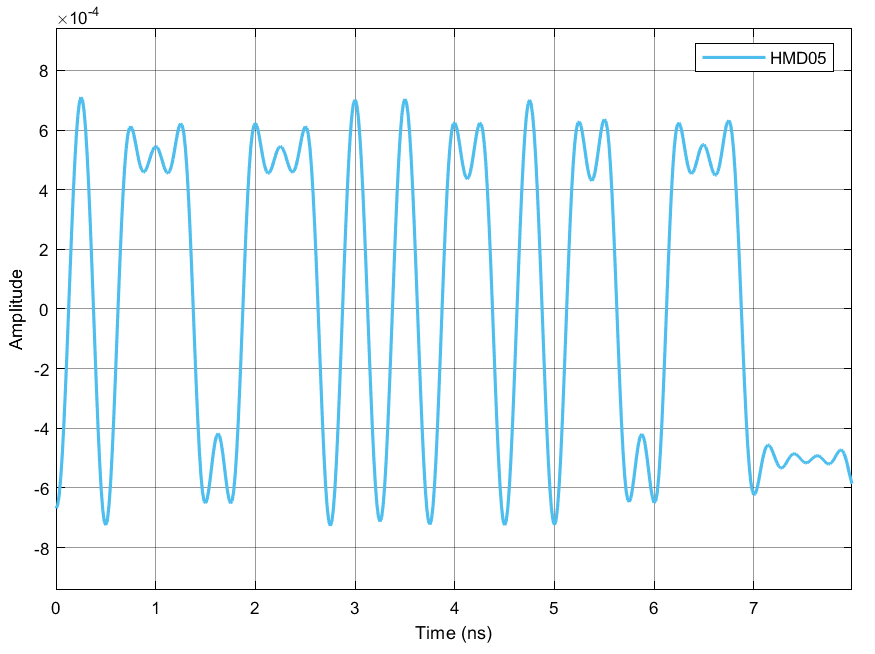
\includegraphics[width=1\textwidth]		
		{./sdf/m_qam_system/figures/simulations/02_thermal/HMD05.pdf}
		\subcaption{}\label{fig:sim_thermalHmd05}
	\end{minipage}
	\begin{minipage}{0.45\textwidth}
		\centering
		\includegraphics[width=1\textwidth]
		{sdf/m_qam_system/figures/simulations/02_thermal/HMD06.pdf}
		\subcaption{}\label{fig:sim_thermalHmd06}
	\end{minipage}
	\caption{Signals HMD05~(\subref{fig:sim_thermalHmd05}) and 
		HMD06~(\subref{fig:sim_thermalHmd06}), outputs of the 
		photodiodes.}\label{fig:sim_thermalHmd0506}
\end{figure}

In this case no signal amplification is used, so there is no amplifier gain or 
noise. This means that the electrical signal will be much smaller than in the 
previous case. This can be verified by comparing 
Figures~\ref{fig:sim_thermalHmd0910} and~\ref{fig:ISIhmd0910}.

	\begin{figure}[H]
	\centering
	\begin{minipage}{0.45\textwidth}
		\centering
		\includegraphics[width=1\textwidth]		
		{./sdf/m_qam_system/figures/simulations/02_thermal/HMD09.pdf}
		\subcaption{}\label{fig:sim_thermalHmd09}
	\end{minipage}
	\begin{minipage}{0.45\textwidth}
		\centering
		\includegraphics[width=1\textwidth]
		{sdf/m_qam_system/figures/simulations/02_thermal/HMD10.pdf}
		\subcaption{}\label{fig:sim_thermalHmd10}
	\end{minipage}
	\caption{Signals HMD09~(\subref{fig:sim_thermalHmd09}) and 
		HMD10~(\subref{fig:sim_thermalHmd10}), after the root-raised-cosine matched 
		filter. They are now following a raised-cosine 
		shape.}\label{fig:sim_thermalHmd0910}
\end{figure}

The thermal noise is then added after the matched filter. As it is only added 
at this point, it is not attenuated or filtered before the sampling process.

	\begin{figure}[H]
	\centering
	\begin{minipage}{0.45\textwidth}
		\centering
		\includegraphics[width=1\textwidth]		
		{./sdf/m_qam_system/figures/simulations/02_thermal/HMD13.pdf}
		\subcaption{}\label{fig:sim_thermalHmd13}
	\end{minipage}
	\begin{minipage}{0.45\textwidth}
		\centering
		\includegraphics[width=1\textwidth]
		{sdf/m_qam_system/figures/simulations/02_thermal/HMD14.pdf}
		\subcaption{}\label{fig:sim_thermalHmd14}
	\end{minipage}
	\caption{Signals HMD13~(\subref{fig:sim_thermalHmd13}) and 
		HMD14~(\subref{fig:sim_thermalHmd14}), after adding thermal 
		noise with an RMS voltage amplitude of $1.6008 \times 10^{-4}$ 
		V.}\label{fig:sim_thermalHmd1314}
\end{figure}

	\begin{figure}[H]
	\centering
	\begin{minipage}{0.45\textwidth}
		\centering
		\includegraphics[width=1\textwidth]		
		{./sdf/m_qam_system/figures/simulations/02_thermal/HMD13ed.pdf}
		\subcaption{}\label{fig:sim_thermalHmd13ed}
	\end{minipage}
	\begin{minipage}{0.45\textwidth}
		\centering
		\includegraphics[width=1\textwidth]
		{sdf/m_qam_system/figures/simulations/02_thermal/HMD14ed.pdf}
		\subcaption{}\label{fig:sim_thermalHmd14ed}
	\end{minipage}
	\caption{Eye diagrams of signals HMD13~(\subref{fig:sim_thermalHmd13ed}) and 
		HMD14~(\subref{fig:sim_thermalHmd14ed}), after adding thermal 
		noise with an RMS voltage amplitude of $1.6008 \times 10^{-4}$ 
		V.}\label{fig:sim_thermalHmd1314ed}
\end{figure}

Figure~\ref{fig:thermalConsts} shows the final received constellations. Two 
things are worth noting:

\begin{itemize}
\item The amplitude of the received constellation points 
($~1\times 10^{-3}$) is much smaller than the initial constellation due to 
the lack of any amplification;
\item The received signal and constellations are strongly affected by noise. 
The thermal noise is not a particularly strong source of noise: However, as the 
signal has not been amplified, they have comparable values.
\end{itemize}


	\begin{figure}[H]
	\centering
		\begin{minipage}{0.45\textwidth}
		\centering
		\includegraphics[width=1\textwidth]
		{sdf/m_qam_system/figures/simulations/02_thermal/constFinal_full.pdf}
		\subcaption{}\label{fig:thermalConstsFull}
	\end{minipage}
	\begin{minipage}{0.45\textwidth}
	\centering
	\includegraphics[width=1\textwidth]
	{sdf/m_qam_system/figures/simulations/02_thermal/constFinal.pdf}
	\subcaption{}\label{fig:thermalConstsSingle}
	\end{minipage}
	\caption{(\subref{fig:thermalConstsFull}) Comparison of transmitted and 
		received constellations. (\subref{fig:thermalConstsSingle}) Constellation 
		of 
		the decoded 
		signals.  Signal optical output power of 0 dBm and 30 km of 
		fiber length (-6 dBm at receiver input).}\label{fig:thermalConsts}
\end{figure}

The signals shown so far had an optical output power of -6 dBm. By 
attenuating using various fiber lengths, we plot a BER curve to study
receiver sensitivity. Receiver sensitivity is usually defined as the minimum 
signal optical power required to achieve a certain BER performance 
\cite{hui09}. The target BER used to measure the sensitivity may vary, and is 
usually chosen considering a desired minimum performance. For instance, in some 
cases a BER smaller than $10^{-12}$ may be desirable to ensure a very low error 
rate. In other cases, the requirement may be only $10^{-3}$ in order for the 
FEC to be effective.

In our case, there is no FEC, and the target BER value can 
be arbitrarily chosen to compare the different configurations. Therefore, we 
use choose to consider the minimum optical signal power required to reach a BER 
of $10^{-3}$. This choice was made in order to allow reaching the values 
relatively quick, with a small confidence interval. This way, generating $10^5$ 
bits we can get an average of 100 errors, which is important for the 
measurement precision. In order to achieve the same with a BER of 
$10^{-6}$ we would need to generate $10^8$ bits, likely requiring several days 
to obtain a single datapoint from the simulation.

%The sensitivity for this configuration is -4.175 dBm.

	\begin{figure}[H]
	\centering
	\includegraphics[width=1\textwidth]
	{sdf/m_qam_system/figures/simulations/02_thermal/berVsOpticalPower.pdf}
	\caption{BER curve of the receiver with thermal 
	noise.}\label{fig:sim_thermal_berVsOpticalPower}
\end{figure}

The theoretical curve was obtained with

\begin{equation}\label{eq:berAN}
\text{BER} = \frac{1}{2} \text{erfc} \left(\frac{A}{\sqrt{2 N}}\right) 
\end{equation}

with

\begin{align*}
A &= \eta K \sqrt{P_{LO} P_s e^{-L\alpha}} \\
N &= {4 k_B T B R}
\end{align*}

\noindent where $\eta$ is the responsivity, $P_s$ is the optical output power, 
$P_{LO}$ is the local oscillator optical output power, $L$ is the fiber length, 
$\alpha$ is the attenuation constant and K is a constant related to the matched 
filter energy. The thermal noise power $N$ is calculated as shown, where $k_B$ 
is the Boltzmann constant, T is the absolute temperature in Kelvin, B is the 
bandwidth and $R$ is the resistance.

For the sensitivity value to meaningful, in addition to the power and BER we 
should also specify the conditions in which those values were measured in the 
receiver, such as the data rate. We can therefore say the sensibility values 
presented here are obtained for a BER of $10^-3$, using a 4 GBd QPSK.

The sensitivity considering the thermal noise establishes the baseline 
sensitivity upon which to compare the rest of them. In the mentioned 
conditions, we have measured a sensibility of -6.1 dBm when using no 
amplification. We can use this value to compare with the rest of the 
simulations, in order to quantify the increased performance provided by 
improvements on the system.



\subsubsection{Simulation results - Electrical Noise}\label{sec:simRes_eNoise}

Keeping the thermal noise, we will now add a transimpedance amplifier after 
each photodiode. The amplifier has a certain bandwidth, gain and input referred 
noise. We assume that the noise gain is equal to the signal gain in this 
amplifier.

	\begin{longtable}[h]{|l|l|l|}
	\caption{Simulation parameters\label{tab:simParams_eNoise_varAmp}}\\\hline
	\textbf{Parameter}            & \textbf{Value}       &\textbf{Units}\\\hline
	numberOfBitsGenerated         & $100 \times 10^3$    & \\\hline
	samplingRate                  & $64 \times 10^9$     & Hz \\\hline
	symbolRate                    & $4 \times 10^9$      & Bd \\\hline
	samplesPerSymbol              & 16                   & \\\hline
	symbolPeriod                  & $250\times 10^{-12}$ & s\\\hline
	bitPeriod                     & $125\times 10^{-12}$ & s\\\hline
	signalOutputPower\_dBm        & -10                  & dBm\\\hline
	localOscillatorPower\_dBm     & 0                    & dBm\\\hline
	localOscillatorPhase          & 0                    & rad\\\hline
	nBw                           & $18\times10^9$       & Hz\\\hline
	responsivity                  & 1                    & A/W\\\hline
	amplification                 & 300    
	              & \\\hline
	amplifierInputNoisePowerSpectralDensity & $1.5657 \times 10^{-19}$ & \\\hline
	thermalNoisePower             & $2.56248 \times 10^{-8}$          & \\\hline
	rxResistance                  & 50 & $\Omega$\\\hline
	temperatureKelvin             & 290 & K\\\hline
	outputFilter                  & RootRaisedCosine     & \\\hline
	shaperFilter                  & RootRaisedCosine     & \\\hline
	rollOffFactor\_out            & 0.9                  & \\\hline
	rollOffFactor\_shp            & 0.9                  & \\\hline
	seedType                      & RandomDevice         & \\\hline
	numberOfBitsReceived          & -1                   & \\\hline
	elFilterType                  & Defined              & \\\hline
	fiberLength\_m                & $50 000$             & m \\\hline
	fiberAttenuation\_m           & 4.6052e-05           & $m^{-1}$ \\\hline
	elFilterOrder                 & 20                   & \\\hline
	opticalGain\_dB               & 0                    & dB \\\hline
	noiseFigure                   & 0                    & dB \\\hline
	bufferLength                  & 512                  & \\\hline
	bitSourceMode                 & Random               & \\\hline
	confidence                    & 0.95                 & \\\hline
\end{longtable}



The addition of an amplifier helps the overcome the thermal noise. 
Nevertheless, it introduces another noise source which also limits the receiver 
performance. This noise source, however, is proportional to the amplifier gain, 
so increasing the gain to very high values does not improve the sensitivity of 
the receiver.

We shall now examine the differences to the previous case. The signals up to 
the photodiodes in the receiver are similar to the previous cases. Therefore, 
we will start by showing the signals at the photodiodes. They are similar to 
the previous cases, but are a point to start.

\begin{figure}[H]
	\centering
	\begin{minipage}{0.45\textwidth}
		\centering
		\includegraphics[width=1\textwidth]		
		{./sdf/m_qam_system/figures/simulations/03_eNoise/HMD05.pdf}
		\subcaption{}\label{fig:sim_eNoiseHmd05}
	\end{minipage}
	\begin{minipage}{0.45\textwidth}
		\centering
		\includegraphics[width=1\textwidth]
		{sdf/m_qam_system/figures/simulations/03_eNoise/HMD06.pdf}
		\subcaption{}\label{fig:sim_eNoiseHmd06}
	\end{minipage}
	\caption{Signals HMD05~(\subref{fig:sim_eNoiseHmd05}) and 
		HMD06~(\subref{fig:sim_eNoiseHmd06}), after detection in the 
		photodiodes.}\label{fig:sim_eNoiseHmd0506}
\end{figure}


\begin{figure}[H]
	\centering
	\begin{minipage}{0.45\textwidth}
		\centering
		\includegraphics[width=1\textwidth]		
		{./sdf/m_qam_system/figures/simulations/03_eNoise/HMD05_ed.pdf}
		\subcaption{}\label{fig:sim_eNoiseHmd05ed}
	\end{minipage}
	\begin{minipage}{0.45\textwidth}
		\centering
		\includegraphics[width=1\textwidth]
		{sdf/m_qam_system/figures/simulations/03_eNoise/HMD06_ed.pdf}
		\subcaption{}\label{fig:sim_eNoiseHmd06ed}
	\end{minipage}
	\caption{Eye diagrams of signals HMD05~(\subref{fig:sim_eNoiseHmd05ed}) and 
		HMD06~(\subref{fig:sim_eNoiseHmd06ed}), after detection in the 
		photodiodes. Shaped with a root-raised cosine 
		filter.}\label{fig:sim_eNoiseHmd0506ed}
\end{figure}

The main difference between previous cases and this one is the existence of an 
amplifier after the photodiodes. This amplifier has three properties which 
affect the signal: a gain, an input referred noise source, and a bandwidth. The 
bandwidth is much larger than the signal bandwidth, and therefore does not have 
any appreciable effects other than limiting the noise bandwidth. The main 
effects of the amplifier, as 
shown in Figures~\ref{fig:sim_eNoiseHmd0708} and~\ref{fig:sim_eNoiseHmd0708ed}, 
are the amplification of the signal and the introduction of noise. The noise 
standard deviation increases proportionally to the amplifier gain.

\begin{figure}[H]
	\centering
	\begin{minipage}{0.45\textwidth}
		\centering
		\includegraphics[width=1\textwidth]		
		{./sdf/m_qam_system/figures/simulations/03_eNoise/HMD07.pdf}
		\subcaption{}\label{fig:sim_eNoiseHmd07}
	\end{minipage}
	\begin{minipage}{0.45\textwidth}
		\centering
		\includegraphics[width=1\textwidth]
		{sdf/m_qam_system/figures/simulations/03_eNoise/HMD08.pdf}
		\subcaption{}\label{fig:sim_eNoiseHmd08}
	\end{minipage}
	\caption{Signals HMD07~(\subref{fig:sim_eNoiseHmd07}) and 
		HMD08~(\subref{fig:sim_eNoiseHmd08}), after detection in the 
		photodiodes.}\label{fig:sim_eNoiseHmd0708}
\end{figure}


\begin{figure}[H]
	\centering
	\begin{minipage}{0.45\textwidth}
		\centering
		\includegraphics[width=1\textwidth]		
		{./sdf/m_qam_system/figures/simulations/03_eNoise/HMD07_ed.pdf}
		\subcaption{}\label{fig:sim_eNoiseHmd07ed}
	\end{minipage}
	\begin{minipage}{0.45\textwidth}
		\centering
		\includegraphics[width=1\textwidth]
		{sdf/m_qam_system/figures/simulations/03_eNoise/HMD08_ed.pdf}
		\subcaption{}\label{fig:sim_eNoiseHmd08ed}
	\end{minipage}
	\caption{Eye diagrams of signals HMD07~(\subref{fig:sim_eNoiseHmd07ed}) and 
		HMD08~(\subref{fig:sim_eNoiseHmd08ed}), after detection in the 
		photodiodes.}\label{fig:sim_eNoiseHmd0708ed}
\end{figure}

The new noise source is placed prior to the matched filter. As such, the noise 
is strongly attenuated when the signal goes through the matched filter. This 
can be seen particularly well by comparing the eye diagrams of 
Figures~\ref{fig:sim_eNoiseHmd0708ed} and~\ref{fig:sim_eNoiseHmd0910ed}. In the 
latter, the eye is widely open when compared to the former, and the variations 
in the signal due to noise are much smoother.

\begin{figure}[H]
	\centering
	\begin{minipage}{0.45\textwidth}
		\centering
		\includegraphics[width=1\textwidth]		
		{./sdf/m_qam_system/figures/simulations/03_eNoise/HMD09.pdf}
		\subcaption{}\label{fig:sim_eNoiseHmd09}
	\end{minipage}
	\begin{minipage}{0.45\textwidth}
		\centering
		\includegraphics[width=1\textwidth]
		{sdf/m_qam_system/figures/simulations/03_eNoise/HMD10.pdf}
		\subcaption{}\label{fig:sim_eNoiseHmd10}
	\end{minipage}
	\caption{Signals HMD09~(\subref{fig:sim_eNoiseHmd09}) and 
		HMD10~(\subref{fig:sim_eNoiseHmd10}), after detection in the 
		photodiodes.}\label{fig:sim_eNoiseHmd0910}
\end{figure}


\begin{figure}[H]
	\centering
	\begin{minipage}{0.45\textwidth}
		\centering
		\includegraphics[width=1\textwidth]		
		{./sdf/m_qam_system/figures/simulations/03_eNoise/HMD09_ed.pdf}
		\subcaption{}\label{fig:sim_eNoiseHmd09ed}
	\end{minipage}
	\begin{minipage}{0.45\textwidth}
		\centering
		\includegraphics[width=1\textwidth]
		{sdf/m_qam_system/figures/simulations/03_eNoise/HMD10_ed.pdf}
		\subcaption{}\label{fig:sim_eNoiseHmd10ed}
	\end{minipage}
	\caption{Eye diagrams of signals HMD09~(\subref{fig:sim_eNoiseHmd09ed}) and 
		HMD10~(\subref{fig:sim_eNoiseHmd10ed}), after detection in the 
		photodiodes.}\label{fig:sim_eNoiseHmd0910ed}
\end{figure}

Lastly, thermal noise is added prior to sampling. However, as can be seen in 
Figures~\ref{fig:sim_eNoiseHmd1314} and~\ref{fig:sim_eNoiseHmd1314ed}, thermal 
noise is negligible in this case, as the signal has been amplified to several 
order of magnitude above the thermal noise level.

\begin{figure}[H]
	\centering
	\begin{minipage}{0.45\textwidth}
		\centering
		\includegraphics[width=1\textwidth]		
		{./sdf/m_qam_system/figures/simulations/03_eNoise/HMD13.pdf}
		\subcaption{}\label{fig:sim_eNoiseHmd13}
	\end{minipage}
	\begin{minipage}{0.45\textwidth}
		\centering
		\includegraphics[width=1\textwidth]
		{sdf/m_qam_system/figures/simulations/03_eNoise/HMD14.pdf}
		\subcaption{}\label{fig:sim_eNoiseHmd14}
	\end{minipage}
	\caption{Signals HMD13~(\subref{fig:sim_eNoiseHmd13}) and 
		HMD14~(\subref{fig:sim_eNoiseHmd14}), after detection in the 
		photodiodes.}\label{fig:sim_eNoiseHmd1314}
\end{figure}


\begin{figure}[H]
	\centering
	\begin{minipage}{0.45\textwidth}
		\centering
		\includegraphics[width=1\textwidth]		
		{./sdf/m_qam_system/figures/simulations/03_eNoise/HMD13_ed.pdf}
		\subcaption{}\label{fig:sim_eNoiseHmd13ed}
	\end{minipage}
	\begin{minipage}{0.45\textwidth}
		\centering
		\includegraphics[width=1\textwidth]
		{sdf/m_qam_system/figures/simulations/03_eNoise/HMD14_ed.pdf}
		\subcaption{}\label{fig:sim_eNoiseHmd14ed}
	\end{minipage}
	\caption{Eye diagrams of signals HMD13~(\subref{fig:sim_eNoiseHmd13ed}) and 
		HMD14~(\subref{fig:sim_eNoiseHmd14ed}), after detection in the 
		photodiodes.}\label{fig:sim_eNoiseHmd1314ed}
\end{figure}

We then get the constellation shown in 
Figure~\ref{fig:eNoise_varAmp_constFinal}. Comparing with 
Figure~\ref{fig:thermalConsts} from the previous section, they appear to have a 
similar signal to noise ratio. While this might be true, it's worth noting that 
the constellation shown here has a much higher amplitude, equal to the 
constellation at the transmitter. In addition, it was obtained with a much 
weaker signal, -20 dBm, compared with 0 dBm in the previous example.

\begin{figure}[H]
	\centering
	\includegraphics[width=0.5\textwidth]
	{sdf/m_qam_system/figures/simulations/03_eNoise/constFinal.pdf}
	\caption{Final constellation. Signal optical output power of -20 dBm and 20 
	km of fiber length (-24 dBm at receiver 
	input).}\label{fig:eNoise_varAmp_constFinal}
\end{figure}

We can compare the results obtained here with the results from the previous 
section, where there was no amplification and only thermal noise was present. 
It is clear that the use of the amplifier leads to much better results.

	\begin{figure}[H]
	\centering
	\includegraphics[width=1\textwidth]
	{sdf/m_qam_system/figures/simulations/03_eNoise/berVsOpticalPower.pdf}
	\caption{BER curve. LO power at 0 dBm, amplifier gain set at 
	300.}\label{fig:eNoise_varAmp_berVsOpticalPower}
\end{figure}

The sensitivity at BER = $10^{-3}$ in these conditions is -22.1 dBm, which is 
quite an improvement over the unamplified scenario.

It is worth noting that the results shown here do not use the same 
amplification for all data points. Instead, the amplification in each point is 
chosen so that the signal amplitude at sampling time is equal to 1, in order to 
replicate the initial constellation.
Taking this into account, first we need to obtain the equation for the 
amplifier gain necessary to make the average of the constellation points have 
the desired value $pm A_g$ (in this case, $A_g = 1$, as it is the case on the 
initial constellation).

\begin{equation}
G_e = \frac{A_g}{\eta K \sqrt{P_s e^{-L\alpha}P_{LO}}}
\end{equation}

The curve can now be obtained with Equation~\ref{eq:berAN}, with

\begin{equation}\label{eq:berANAmped}
\begin{split}
	A &= \eta G_e K \sqrt{ P_s P_{LO} e^{-L\alpha}}\\
	N &= {4 k_B T B R} + \left(\sqrt{n_{in} \frac{1}{T_s}} G_e K\right)^2
\end{split}
\end{equation}

All variables are as previously defined. In addition, $T_s$ is the symbol 
period of the transmitted signal and $n_{in}$ is the input referred noise 
spectral density of the transimpedance amplifier.



	\begin{figure}[H]
	\centering
	\includegraphics[width=1\textwidth]
	{sdf/m_qam_system/figures/simulations/03_eNoise/berVsAmpGain.pdf}
	\caption{BER as a function of the transimpedance amplifier 
	gain, along with the curves where the individual noise sources dominate. 
	Signal output power of -25 dBm and local oscillator power of 0 dBm.
	}\label{fig:eNoise_varAmp_berVsAmpGain}
\end{figure}

	\begin{figure}[H]
	\centering
	\includegraphics[width=1\textwidth]
	{sdf/m_qam_system/figures/simulations/03_eNoise/berVsAmpGain_6dBm.pdf}
	\caption{BER as a function of the transimpedance amplifier 
		gain, along with the curves where the individual noise sources dominate. 
		Signal output power of -6 dBm and local oscillator power of 0 dBm.
	}\label{fig:eNoise_varAmp_berVsAmpGain6dBm}
\end{figure}

We can see the direct effect of the amplifier on the BER on 
Figure~\ref{fig:eNoise_varAmp_berVsAmpGain}.
The yellow curve is the expected behavior if thermal noise was the only noise 
source. It 
better demonstrates the system behavior at low gains, 
reflecting the case where the thermal noise 
overwhelms the amplifier-generated noise. As 
the gain increases, the thermal noise component becomes less significant when 
compared to the signal and to the amplifier noise. When the gain is high enough 
($10^2$ in the plot), thermal noise is negligible when compared to the 
amplifier output, and system follows the purple line. This line shows the 
expected behavior if the only noise present was due to the amplifier. At this 
point, the 
performance limiting factor is the relation between the current 
generated at the photodiodes and the input referred noise of the amplifiers. 
This ratio is constant and independent from the gain.

	\begin{figure}[H]
	\centering
	\includegraphics[width=1\textwidth]
	{sdf/m_qam_system/figures/simulations/03_eNoise/berVsOpticalPowerVar.pdf}
	\caption{Comparison of BER curves with different gains. Local oscillator 
	power of 0 dBm. We can see that when G=1, the curve is similar to the case 
	without amplifier shown in 
	Figure~\ref{fig:sim_thermal_berVsOpticalPower}}\label{fig:eNoise_varAmp_berCurveAmpGainVar}
\end{figure}

\begin{figure}[h]
	\centering
	\begin{minipage}{0.33\textwidth}
		\centering
		\includegraphics[width=1\textwidth]{sdf/m_qam_system/figures/simulations/03_eNoise/constFinal_G5_20km.pdf}
		\subcaption{$G = 5$}
	\end{minipage}
	\begin{minipage}{0.33\textwidth}
		\centering
		\includegraphics[width=1\textwidth]{sdf/m_qam_system/figures/simulations/03_eNoise/constFinal_G10_20km.pdf}
		\subcaption{$G = 10$}
	\end{minipage}
	\begin{minipage}{0.33\textwidth}
		\centering
		\includegraphics[width=1\textwidth]{sdf/m_qam_system/figures/simulations/03_eNoise/constFinal_G100_20km.pdf}
		\subcaption{$G = 100$}
	\end{minipage}
	\begin{minipage}{0.33\textwidth}
		\centering
		\includegraphics[width=1\textwidth]{sdf/m_qam_system/figures/simulations/03_eNoise/constFinal_G1000_20km.pdf}
		\subcaption{$G = 1000$}
	\end{minipage}
	\caption{Final constellations for various local oscillator optical 
		powers. Signal optical power at is -15 
		dBm, with 20 km of fiber length (-19 dBm at receiver 
		input). It is easy to see that there does not appear to be a significant 
		improvement between the constellations with the gains of 100 and 
		1000.}\label{fig:sim_eNoise_consts}
\end{figure}

\clearpage


\subsubsection{Simulation results - Increased LO}\label{sec:simRes_incLO}

As mentioned in the previous section, one way to further increase performance 
is to improve the relation between the current generated at the photodiodes and 
the input referred noise of the amplifiers. This can be done by using a higher 
optical power on the Local Oscillator. Thus, the current generated at the 
current generated at the photodiodes will be increased.

	\begin{longtable}[h]{|l|l|l|}
	\caption{Simulation parameters\label{tab:simParams_incLO}}\\\hline
	\textbf{Parameter}            & \textbf{Value}       &\textbf{Units}\\\hline
	numberOfBitsGenerated         & $100 \times 10^3$    & \\\hline
	samplingRate                  & $64 \times 10^9$     & Hz \\\hline
	symbolRate                    & $4 \times 10^9$      & Bd \\\hline
	samplesPerSymbol              & 16                   & \\\hline
	symbolPeriod                  & $250\times 10^{-12}$ & s\\\hline
	bitPeriod                     & $125\times 10^{-12}$ & s\\\hline
	signalOutputPower\_dBm        & -20                  & dBm\\\hline
	localOscillatorPower\_dBm     & 5                    & dBm\\\hline
	localOscillatorPhase          & 0                    & rad\\\hline
	nBw                           & $18\times10^9$       & Hz\\\hline
	responsivity                  & 1                    & A/W\\\hline
	amplification                 & 300                  & \\\hline
	amplifierInputNoisePowerSpectralDensity & $1.5657 \times 10^{-19}$ & \\\hline
	thermalNoisePower             & $2.56248 \times 10^{-8}$          & \\\hline
	rxResistance                  & 50 & $\Omega$\\\hline
	temperatureKelvin             & 290 & K\\\hline
	outputFilter                  & RootRaisedCosine     & \\\hline
	shaperFilter                  & RootRaisedCosine     & \\\hline
	rollOffFactor\_out            & 0.9                  & \\\hline
	rollOffFactor\_shp            & 0.9                  & \\\hline
	seedType                      & RandomDevice         & \\\hline
	numberOfBitsReceived          & -1                   & \\\hline
	elFilterType                  & Defined              & \\\hline
	fiberLength\_m                & $20 000$             & m \\\hline
	fiberAttenuation\_m           & 4.6052e-05           & $m^{-1}$ \\\hline
	elFilterOrder                 & 20                   & \\\hline
	opticalGain\_dB               & 0                    & dB \\\hline
	noiseFigure                   & 0                    & dB \\\hline
	bufferLength                  & 512                  & \\\hline
	bitSourceMode                 & Random               & \\\hline
	confidence                    & 0.95                 & \\\hline
\end{longtable}

The increased current at the photodiodes' output means that the same amplitude 
can be reached with a lower amplifier gain. A lower gain, by itself, implies 
that the input referred noise of the amplifier will stay at a lower value, 
thereby increasing the sensitivity of the system.
In this example, the signals will not be shown here, as the only difference is 
that the amplitude of the signal after the photodiodes is higher.

\begin{figure}[H]
	\centering
	\includegraphics[width=0.5\textwidth]
	{sdf/m_qam_system/figures/simulations/04_incLO/constFinal.pdf}
	\caption{Final constellation (normalized). Signal optical output power of -20 
	dBm and 20 
		km of fiber length (-24 dBm at receiver 
		input). Local oscillator at 5 dBm.}\label{fig:incLO_constFinal}
\end{figure}

In Figure~\ref{fig:incLO_constFinal} we can see the final constellation 
obtained when choosing an output optical power of -20 dBm and setting the fiber 
length to 20 km. In conditions similar to 
Figure~\ref{fig:eNoise_varAmp_constFinal} it shows a much better constellation. 
This is all due to the higher local oscillator value.



	\begin{figure}[H]
	\centering
	\includegraphics[width=1\textwidth]
	{sdf/m_qam_system/figures/simulations/04_incLO/berComp.pdf}
	\caption{Comparison of BER curves: considering thermal noise only, using an 
	electrical amplifier, and using a higher value of local 
	oscillator together with the amplifier. Amplifier gain was set at 
	300.}\label{fig:sim_incLO_ber12dBm}
\end{figure}

The sensitivity of the new curve, at BER $10^{-3}$,with local oscillator power 
of 5 dBm, is -27.1 dBm, 5 dB lower than the curve with the LO at 0 dBm.

The theoretical curve in Figure~\ref{fig:sim_incLO_ber12dBm} was obtained 
according to the same equation as the second curve in the previous section. 
Notice that the new curve is approximately 5 dB to the left of curve with the 
amplifier and the LO at 0 dBm. This is because in the 
equations~\ref{eq:berAN} and~\ref{eq:berANAmped}, the power of the local 
oscillator is as important as the optical signal power, and the amplitude at 
sampling time grows at the same rate with both quantities.

	\begin{figure}[h]
	\centering
	\includegraphics[width=1\textwidth]
	{sdf/m_qam_system/figures/simulations/04_incLO/berCurveVarLO.pdf}
	\caption{Variation of BER with the LO power. Signal optical power at receiver 
	input is -25 dBm.}\label{fig:sim_incLO_varLO}
\end{figure}

\begin{figure}[h]
	\centering
	\begin{minipage}{0.33\textwidth}
		\centering
		\includegraphics[width=1\textwidth]{sdf/m_qam_system/figures/simulations/04_incLO/constNorm_lo0dBm.pdf}
		\subcaption{$P_{lo} = 0$ dBm}
	\end{minipage}
	\begin{minipage}{0.33\textwidth}
		\centering
		\includegraphics[width=1\textwidth]{sdf/m_qam_system/figures/simulations/04_incLO/constNorm_lo3dBm.pdf}
		\subcaption{$P_{lo} = 3$ dBm}
	\end{minipage}
	\begin{minipage}{0.33\textwidth}
		\centering
		\includegraphics[width=1\textwidth]{sdf/m_qam_system/figures/simulations/04_incLO/constNorm_lo6dBm.pdf}
		\subcaption{$P_{lo} = 6$ dBm}
	\end{minipage}
	\begin{minipage}{0.33\textwidth}
		\centering
		\includegraphics[width=1\textwidth]{sdf/m_qam_system/figures/simulations/04_incLO/constNorm_lo20dBm.pdf}
		\subcaption{$P_{lo} = 20$ dBm}
	\end{minipage}
	\caption{Final constellations for various local oscillator optical 
		powers. Signal optical power at receiver input is -25 
		dBm.}\label{fig:sim_loVarConsts}
\end{figure}

This might lead us to believe that by increasing the LO, the performance can be 
improved as much as required. However, that would only be the case if the Local 
	Oscillator was independent from any noise source. That is not the case, as we 
shall see in the next section.

\clearpage

\subsubsection{Simulation results - Quantum 
Noise}\label{sec:simRes_quantumNoise}

We will now consider the more realistic case when there is quantum noise 
associated with the local oscillator. We can consider quantum noise to be 
similar to shot noise.

In this simulation, we will add noise at the photodiodes, where the noise 
current variance will be proportional to total generated photocurrent. 
Normally, shot noise follows a Poisson distribution. However, for the purpose 
of this section, we shall consider that the number of photons is high enough so 
that it can be considered to follow a normal distribution.

\begin{equation}
\sigma_{\text{shot}}^2 = 2 q I B = 2 \eta P_\text{opt} B
\end{equation}

As the local oscillator will be much higher than the signal, we can consider 
that the total optical power generating current is equal to the local 
oscillator power. Due to the optical hybrid, each photodiode receives $1/4$ of 
the local oscillator optical power.

Keeping in mind that the noise and signal will be affected by the same gains, 
the factor which control performance are the signal and noise ratio at the 
photodiodes output, and the matched filter. The other blocks of the receiver 
will have no practical effects, as the LO amplification will render the other 
noise sources negligible, and the matched filter ultimately limits the noise 
bandwidth.

We then have that the signal current amplitude at the photodiode's output is 
given by:

\begin{equation}
	A = \eta \sqrt{ P_{LO} P_s }
\end{equation}


On the other hand, the shot noise variance $N_\text{shot i}$ in each photodiode 
will be given by

\begin{equation}
	N_{\text{shot i}} = 2 \eta h f \frac{P_{LO}}{4} B
\end{equation}

\noindent with $2 B = 1/\tau$, where $\tau$ is the sampling period.

Considering the shot noise to be approximated as a gaussian random 
variable, the noise at output of each pair of photodiodes can be obtained by 
the sum of their variances:

\begin{equation}
	\begin{split}
		N_{\text{shot}} &= N_{\text{shot 1}} + N_{\text{shot 2}} \\
										&\approxeq 2 N_{\text{shot i}} =\\
										&= 4 \eta h f \frac{P_{LO}}{4} B
	\end{split}
\end{equation}

We can now calculate $A$ and $N$ after the matched filter output:

\begin{equation}
	\begin{split}
		A &= \eta G_e K \sqrt{ P_s P_{LO} e^{-L\alpha}}\\
		N &= {4 k_B T B R} + \left(\sqrt{n_{in} \frac{1}{T_s}} G_e K\right)^2 +
		 \left(\sqrt{\frac{N_{\text{shot}}}{B} \frac{1}{T_s}} G_e K\right)^2
	\end{split}
\end{equation}

	\begin{figure}[h]
	\centering
	\includegraphics[width=1\textwidth]
	{sdf/m_qam_system/figures/simulations/05_loShot/berCurve_loShotVar.pdf}
	\caption{Variation of BER with the LO power, with shot noise. Signal optical 
	power at receiver 
		input is -56 dBm.}\label{fig:sim_loShot_varLO}
\end{figure}

In addition, we can compare these results with the quantum limit. The quantum 
limit establishes the absolute minimum sensitivity of the receiver, and varies 
according to the modulation scheme and type of detector. In the case of QPSK 
with homodyne detection this limit is given by~\cite{senior09, agrawal12}:

\begin{equation}\label{eq:quantumLimit_homodyne}
\text{BER} = \frac{1}{2} \text{erfc}\left( \sqrt{2 \eta_q N_p}\right)
\end{equation}

\noindent where $eta_q$ is the quantum efficiency of the receiver, and $N_p$ is 
the number of photons per bit. We can convert the average number of photons per 
bit to dBm or vice versa:

\begin{align}
	P_{\text{dBm}} = 10 \log_{10}\left(\frac{h f}{T_b} N_p \times 10^3\right) \\
	N_p = \frac{10^{(P_{\text{dBm}}/10)} T_b \times 10^{-3}}{hf}
\end{align}

It is worth remembering that we are neglecting most effects which arise due to 
working with a small number of photons, and just assuming that the system 
behaves similarly as for larger numbers of photons.

	\begin{figure}[h]
	\centering
	\includegraphics[width=1\textwidth]
	{sdf/m_qam_system/figures/simulations/05_loShot/berCurve_loShot2.pdf}
	\caption{BER variation with the optical power. $P_{lo} = 50$ dBm 
	.}\label{fig:sim_loShot_quantumLimit}
\end{figure}

We can see that in this case the sensitivity at a BER $10^{-3}$ is -56 dBm, 
which is at the quantum limit. This corresponds to an average of 2.4 photons 
per bit.

%
%The main 
%difference is on the signal after the matched filter, which is affected by 
%noise. Signals HMD09 and HMD10 then become as shown in 
%Figures~\ref{fig:sim_thermalHmd0910} and~\ref{fig:sim_thermalHmd0910ed}.
%
%	\begin{figure}[H]
%	\centering
%	\begin{minipage}{0.45\textwidth}
%		\centering
%		\includegraphics[width=1\textwidth]		
%		{./sdf/m_qam_system/figures/simulations/02_thermal/HMD09.pdf}
%		\subcaption{}\label{fig:sim_thermalHmd09}
%	\end{minipage}
%	\begin{minipage}{0.45\textwidth}
%		\centering
%		\includegraphics[width=1\textwidth]
%		{sdf/m_qam_system/figures/simulations/02_thermal/HMD10.pdf}
%		\subcaption{}\label{fig:sim_thermalHmd10}
%	\end{minipage}
%	\caption{Eye diagrams for HMD09~(\subref{fig:ISIhmd09ed}) and 
%		HMD10~(\subref{fig:ISIhmd10ed}), after the root-raised-cosine matched 
%		filter. They are now following a raised-cosine 
%		shape.}\label{fig:sim_thermalHmd0910}
%\end{figure}
%
%	\begin{figure}[H]
%	\centering
%	\begin{minipage}{0.45\textwidth}
%		\centering
%		\includegraphics[width=1\textwidth]		
%		{./sdf/m_qam_system/figures/simulations/02_thermal/HMD09_ed.pdf}
%		\subcaption{}\label{fig:sim_thermalHmd09ed}
%	\end{minipage}
%	\begin{minipage}{0.45\textwidth}
%		\centering
%		\includegraphics[width=1\textwidth]
%		{sdf/m_qam_system/figures/simulations/02_thermal/HMD10_ed.pdf}
%		\subcaption{}\label{fig:sim_thermalHmd10ed}
%	\end{minipage}
%	\caption{Eye diagrams for HMD09~(\subref{fig:ISIhmd09ed}) and 
%		HMD10~(\subref{fig:ISIhmd10ed}), after the root-raised-cosine matched 
%		filter. They are now following a raised-cosine 
%		shape.}\label{fig:sim_thermalHmd0910ed}
%\end{figure}


%\subsubsection{Simulation results - Electrical Noise}\label{sec:simRes_eNoise}
%
%After showing that the implemented shaping process does not create any 
%inter-symbol interference, we will now verify the effects of electrical noise.
%This noise currently has two components:
%
%\begin{itemize}
%	\item The transimpedance amplifier block generates electrical noise dependent 
%	on the gain. In real world datasheets, this noise is quantified as, for 
%	instance, an input referred noise current. This current is then amplified, 
%	depending on the gain of the amplifier. In model we use, the gain is equal 
%	for the signal and for the noise.
%	\item White noise modeling thermal voltage noise is also generated after the 
%	amplifier, and added to the signal.
%\end{itemize}
%
%We shall see the effects of these noise sources, and how they affect 
%the simulated system's performance.
%
%	\begin{longtable}[h]{|l|l|l|}
%	\caption{Simulation parameters\label{tab:fiberThermalParams}}\\\hline
%	\textbf{Parameter}            & \textbf{Value}       &\textbf{Units}\\\hline
%	numberOfBitsGenerated         & $100 \times 10^3$    & \\\hline
%	samplingRate                  & $64 \times 10^9$     & Hz \\\hline
%	symbolRate                    & $4 \times 10^9$      & Bd \\\hline
%	samplesPerSymbol              & 16                   & \\\hline
%	symbolPeriod                  & $250\times 10^{-12}$ & s\\\hline
%	bitPeriod                     & $125\times 10^{-12}$ & s\\\hline
%	signalOutputPower\_dBm        & -10                  & dBm\\\hline
%	localOscillatorPower\_dBm     & 0                    & dBm\\\hline
%	localOscillatorPhase          & 0                    & rad\\\hline
%	nBw                           & $18\times10^9$       & Hz\\\hline
%	responsivity                  & 0.05                 & A/W\\\hline
%	amplification                 & 39529.1              & \\\hline
%	amplifierInputNoisePowerSpectralDensity & 3.1314e-23 & \\\hline
%	thermalNoisePowerSpectralDensity& 1.6015520e-18      & \\\hline
%	rxResistance                  & 50 & $\omega$\\\hline
%	temperatureKelvin             & 290 & K\\\hline
%	outputFilter                  & RootRaisedCosine     & \\\hline
%	shaperFilter                  & RootRaisedCosine     & \\\hline
%	rollOffFactor\_out            & 0.9                  & \\\hline
%	rollOffFactor\_shp            & 0.9                  & \\\hline
%	seedType                      & RandomDevice         & \\\hline
%	numberOfBitsReceived          & -1                   & \\\hline
%	elFilterType                  & Defined              & \\\hline
%	fiberLength\_m                & $100 \times 10^3$    & m \\\hline
%	fiberAttenuation\_m           & 4.6052e-05           & $m^{-1}$ \\\hline
%	elFilterOrder                 & 20                   & \\\hline
%	opticalGain\_dB               & 0                    & dB \\\hline
%	noiseFigure                   & 0                    & dB \\\hline
%	preFilterNoiseSpectralDensity & $1 \times 10^-{17}$  & W/Hz\\\hline
%	elNoiseSpectralDensity        & 0                    & W/Hz\\\hline
%	bufferLength                  & 512                  & \\\hline
%	bitSourceMode                 & Random               & \\\hline
%	midReportSize                 & 0                    & \\\hline
%	confidence                    & 0.95                 & \\\hline
%	samplesToSkip                 & 256                  & \\\hline
%\end{longtable}
%
%
%	\begin{figure}[H]
%	\centering
%	\includegraphics[width=0.7\textwidth]
%	{sdf/m_qam_system/figures/simulations/02_eNoise/constFinal.pdf}
%	\caption{Constellation of the encoded and decoded 
%		signals. They coincide, but the received constellation is affected by some 
%		noise.}\label{fig:eNoiseconsts}
%\end{figure}
%
%\subsubsection{Simulation results - Optical Fiber with Electrical 
%	Noise}\label{sec:simRes_eNoiseAtt}
%	
%	Building upon the former example, we shall now increase the 
%	fiber length, while maintaining the electrical amplifier gain and noise 
%	spectral densities. We shall see that keeping these properties constant 
%	establishes a given relation between the optical fiber length and the bit 
%	error rate.
%		
%	Table~\ref{tab:fiberThermalParams} shows the parameters used to obtain the 
%	signals in this section.
%	
%	\begin{longtable}[h]{|l|l|l|}
%		\caption{Simulation parameters\label{tab:fiberThermalParams}}\\\hline
%		\textbf{Parameter}            & \textbf{Value}       &\textbf{Units}\\\hline
%		numberOfBitsGenerated         & $100 \times 10^3$    & \\\hline
%		samplingRate                  & $64 \times 10^9$     & Hz \\\hline
%		symbolRate                    & $4 \times 10^9$      & Bd \\\hline
%		samplesPerSymbol              & 16                   & \\\hline
%		symbolPeriod                  & $250\times 10^{-12}$ & s\\\hline
%		bitPeriod                     & $125\times 10^{-12}$ & s\\\hline
%		signalOutputPower\_dBm        & -10                  & dBm\\\hline
%		localOscillatorPower\_dBm     & 0                    & dBm\\\hline
%		localOscillatorPhase          & 0                    & rad\\\hline
%		nBw                           & $18\times10^9$       & Hz\\\hline
%		amplification                 & 40                   & \\\hline
%		responsivity                  & 0.07                 & A/W\\\hline
%		outputFilter                  & RootRaisedCosine     & \\\hline
%		shaperFilter                  & RootRaisedCosine     & \\\hline
%		rollOffFactor\_out            & 0.9                  & \\\hline
%		rollOffFactor\_shp            & 0.9                  & \\\hline
%		seedType                      & RandomDevice         & \\\hline
%		numberOfBitsReceived          & -1                   & \\\hline
%		elFilterType                  & Defined              & \\\hline
%		fiberLength\_m                & $100 \times 10^3$    & m \\\hline
%		fiberAttenuation\_m           & 4.6052e-05           & $m^{-1}$ \\\hline
%		elFilterOrder                 & 20                   & \\\hline
%		opticalGain\_dB               & 0                    & dB \\\hline
%		noiseFigure                   & 0                    & dB \\\hline
%		preFilterNoiseSpectralDensity & $1 \times 10^-{17}$  & W/Hz\\\hline
%		elNoiseSpectralDensity        & 0                    & W/Hz\\\hline
%		bufferLength                  & 512                  & \\\hline
%		bitSourceMode                 & Random               & \\\hline
%		midReportSize                 & 0                    & \\\hline
%		confidence                    & 0.95                 & \\\hline
%		samplesToSkip                 & 266                  & \\\hline
%	\end{longtable}
%	
%	The optical signals are similar to the ones shown in the previous section, so 
%	we shall skip them. We will start by looking at the signals HMD07 and HMD08, 
%	the amplified version of the signals detected at the photodiodes.
%	
%	\begin{figure}[H]
%		\centering
%		\begin{minipage}{0.45\textwidth}
%			\centering
%			\includegraphics[width=1\textwidth]		
%			{./sdf/m_qam_system/figures/simulations/04_wFiberThermal/HMD07.pdf}
%			\subcaption{}\label{fig:fiberThmd07}
%		\end{minipage}
%		\begin{minipage}{0.45\textwidth}
%			\centering
%			\includegraphics[width=1\textwidth]
%			{sdf/m_qam_system/figures/simulations/04_wFiberThermal/HMD08.pdf}
%			\subcaption{}\label{fig:fiberThmd08}
%		\end{minipage}
%		\caption{Signals HMD07~(\subref{fig:fiberThmd07}) and 
%			HMD08~(\subref{fig:fiberThmd08}), 
%			containing the amplified versions of the signals detected at the 
%			\textit{photodiode} blocks}\label{fig:fiberThmd0708}
%	\end{figure}
%	
%	So far the signals look very similar the previous ones. However, this time we 
%	add Gaussian white noise to model thermal noise at the receiver.
%	
%	\begin{figure}[H]
%		\centering
%		\begin{minipage}{0.45\textwidth}
%			\centering
%			\includegraphics[width=1\textwidth]		
%			{./sdf/m_qam_system/figures/simulations/04_wFiberThermal/HMD11.pdf}
%			\subcaption{}\label{fig:fiberThmd11}
%		\end{minipage}
%		\begin{minipage}{0.45\textwidth}
%			\centering
%			\includegraphics[width=1\textwidth]
%			{sdf/m_qam_system/figures/simulations/04_wFiberThermal/HMD12.pdf}
%			\subcaption{}\label{fig:fiberThmd12}
%		\end{minipage}
%		\caption{Signals HMD1~(\subref{fig:fiberThmd11}) and 
%			HMD12~(\subref{fig:fiberThmd12}), 
%			amplified signals after white adding noise.}\label{fig:fiberThmd1112}
%	\end{figure}
%	
%	The amount of noise is limited by the bandwidth of the electrical filter.
%	
%	\begin{figure}[H]
%		\centering
%		\begin{minipage}{0.45\textwidth}
%			\centering
%			\includegraphics[width=1\textwidth]		
%			{./sdf/m_qam_system/figures/simulations/04_wFiberThermal/HMD13.pdf}
%			\subcaption{}\label{fig:fiberThmd13}
%		\end{minipage}
%		\begin{minipage}{0.45\textwidth}
%			\centering
%			\includegraphics[width=1\textwidth]
%			{sdf/m_qam_system/figures/simulations/04_wFiberThermal/HMD14.pdf}
%			\subcaption{}\label{fig:fiberThmd14}
%		\end{minipage}
%		\caption{Signals HMD13~(\subref{fig:fiberThmd13}) and 
%			HMD14~(\subref{fig:fiberThmd14}), 
%			signals after the electrical filter.}\label{fig:fiberThmd1314}
%	\end{figure}
%	
%	In addition, the matched filter improves the SNR before sampling. However, in 
%	this case, the noise power is too high when compared with the signal.
%	
%	\begin{figure}[H]
%		\centering
%		\begin{minipage}{0.45\textwidth}
%			\centering
%			\includegraphics[width=1\textwidth]		
%			{./sdf/m_qam_system/figures/simulations/04_wFiberThermal/HMD23.pdf}
%			\subcaption{}\label{fig:fiberThmd23}
%		\end{minipage}
%		\begin{minipage}{0.45\textwidth}
%			\centering
%			\includegraphics[width=1\textwidth]
%			{sdf/m_qam_system/figures/simulations/04_wFiberThermal/HMD24.pdf}
%			\subcaption{}\label{fig:fiberThmd24}
%		\end{minipage}
%		\caption{Signals HMD23~(\subref{fig:fiberThmd23}) and 
%			HMD24~(\subref{fig:fiberThmd24}), 
%			signals after the electrical filter.}\label{fig:fiberThmd2324}
%	\end{figure}
%	
%	Looking back at the previous section, the expected amplitude at the 
%	constellation would be close to $2 \times 
%	10^{-3}$. However, looking at Figures~\ref{fig:fiberThmd2324} 
%	and~\ref{fig:fiberTconsts}, we can see that the noise introduces values an 
%	order of magnitude above it, and so it obfuscates the constellation.
%	
%	\begin{figure}[H]
%		\centering
%		\begin{minipage}{0.45\textwidth}
%			\centering
%			\includegraphics[width=1\textwidth]		
%			{./sdf/m_qam_system/figures/simulations/04_wFiberThermal/constStart.pdf}
%			\subcaption{}\label{fig:fiberTconstStart}
%		\end{minipage}
%		\begin{minipage}{0.45\textwidth}
%			\centering
%			\includegraphics[width=1\textwidth]
%			{sdf/m_qam_system/figures/simulations/04_wFiberThermal/constFinal.pdf}
%			\subcaption{}\label{fig:fiberTconstFinal}
%		\end{minipage}
%		\caption{(\subref{fig:fiberTconstStart}) Constellation of the encoded 
%		signal; 
%			(\subref{fig:fiberTconstFinal}) Constellation of the decoded 
%			signal.}\label{fig:fiberTconsts}
%	\end{figure}
%	
%	We can use this to establish a thermal noise sensitivity. Using various fiber 
%	lengths, we can plot a curve of the BER against the fiber length in these 
%	conditions. For this, we can use Equation~\ref{eq:berMod}, with $n_0$ equal 
%	to 
%	the added noise spectral density and $E_b$ given by:
%	
%	\begin{equation}\label{eq:ebFiberLoss}
%	E_b = G_e^2 \eta^2 P_S P_{LO} \frac{T_s}{2} \exp{(-L \alpha)}
%	\end{equation}
%	
%	In this equation, all symbols are as previously defined, L is the fiber 
%	length 
%	and alpha is the attenuation coefficient. Using this, we obtain the curve 
%	shown 
%	in Figure~\ref{fig:fiberTberFiberL}. All points from the simulations were 
%	acquired with the parameters from Table~\ref{tab:fiberThermalParams}, with 
%	the 
%	exception of the \textit{fiberLength\_m}, which was varied from 0 to 200000 m 
%	in intervals of 10000 m.
%	
%	\begin{figure}[H]
%		\centering
%		\includegraphics[width=0.95\textwidth]
%		{sdf/m_qam_system/figures/simulations/04_wFiberThermal/berVsFiber_old.pdf}
%		\caption{BER vs fiber length.}\label{fig:fiberTberFiberL}
%	\end{figure}
%	
%	This electrical noise can be made irrelevant in one of three ways:
%	
%	\begin{itemize}
%		\item Increasing the signal power at the transmitter. This is the most 
%		obvious solution, but does not technically compensate for losses, and might 
%		be undesirable.
%		\item Using an optical preamplifier, as shown in 
%		Section~\ref{sec:simRes_edfa}. If the amplification is high enough, the 
%		signal generated from the optical input will be far more pronounced than 
%		the 
%		electrical noise. This generates optical noise in the process, but is still 
%		typically more advantageous than having a lower optical power at the 
%		receiver 
%		input.
%		\item Increasing the LO power. As seen in Equation~\ref{eq:ebFiberLoss}, 
%		increasing the LO power will proportionately increase the energy per bit.
%	\end{itemize}
%
%In this section we will change the simulation to explore the consequences of 
%two small changes:
%
%\begin{itemize}
%	\item Adding an \textit{optical\_fiber} block after the transmitter, with a 
%	length of 100 km and attenuation coefficient of 0.2 dB/km;
%	\item Adding an EDFA as an optical preamplifier to compensate for the fiber 
%	losses, introducing both 
%	noise and a gain factor.
%\end{itemize}
%
%The location of these blocks can be seen in 
%\ref{fig:MQAM_system_block_diagram}.
%
%Table~\ref{tab:edfaParams} shows the parameters used to obtain the signals
%in this section.
%
%\begin{longtable}[h]{|l|l|l|}
%	\caption{Simulation parameters\label{tab:edfaParams}}\\\hline
%	\textbf{Parameter}            & \textbf{Value}       &\textbf{Units}\\\hline
%	numberOfBitsGenerated         & $100 \times 10^3$    & \\\hline
%	samplingRate                  & $64 \times 10^9$     & Hz \\\hline
%	symbolRate                    & $4 \times 10^9$      & Bd \\\hline
%	samplesPerSymbol              & 16                   & \\\hline
%	symbolPeriod                  & $250\times 10^{-12}$ & s\\\hline
%	bitPeriod                     & $125\times 10^{-12}$ & s\\\hline
%	signalOutputPower\_dBm        & -10                  & dBm\\\hline
%	localOscillatorPower\_dBm     & 0                    & dBm\\\hline
%	localOscillatorPhase          & 0                    & rad\\\hline
%	nBw                           & $18\times10^9$       & Hz\\\hline
%	amplification                 & 40                   & \\\hline
%	responsivity                  & 0.07                 & A/W\\\hline
%	outputFilter                  & RootRaisedCosine     & \\\hline
%	shaperFilter                  & RootRaisedCosine     & \\\hline
%	rollOffFactor\_out            & 0.9                  & \\\hline
%	rollOffFactor\_shp            & 0.9                  & \\\hline
%	seedType                      & RandomDevice         & \\\hline
%	numberOfBitsReceived          & -1                   & \\\hline
%	elFilterType                  & Defined              & \\\hline
%	fiberLength\_m                & $100 \times 10^3$    & m \\\hline
%	fiberAttenuation\_m           & 4.6052e-05           & $m^{-1}$ \\\hline
%	elFilterOrder                 & 20                   & \\\hline
%	opticalGain\_dB               & 20                   & dB \\\hline
%	noiseFigure                   & 4                    & dB \\\hline
%	preFilterNoiseSpectralDensity & 0                    & W/Hz\\\hline
%	elNoiseSpectralDensity        & 0                    & W/Hz\\\hline
%	bufferLength                  & 512                  & \\\hline
%	bitSourceMode                 & Random               & \\\hline
%	midReportSize                 & 0                    & \\\hline
%	confidence                    & 0.95                 & \\\hline
%	samplesToSkip                 & 266                  & \\\hline
%\end{longtable}
%
%
%The transmitter part will be skipped, as for all intents and purposes its 
%properties remain the same from last section. Therefore we start with the 
%optical signal S1, containing the transmitted optical signal at the exit of 
%the 
%\textit{m\_qam\_transmitter} block.
%
%\begin{figure}[H]
%	\centering
%	\centering
%	\includegraphics[width=0.7\textwidth]		
%	{./sdf/m_qam_system/figures/simulations/02_wFiberEdfa/S1.pdf}
%	\caption{Signal S1, modulated optical signal.}\label{fig:EdfaS1}
%\end{figure}
%
%This signal then passes through an \textit{optical\_fiber} block, with the 
%dispersion coefficient set to zero. This attenuates the signal power by 
%approximately 20 dB.
%
%\begin{figure}[H]
%	\centering
%	\centering
%	\includegraphics[width=0.7\textwidth]		
%	{./sdf/m_qam_system/figures/simulations/02_wFiberEdfa/S2l.pdf}
%	\caption{Signal S2, modulated optical signal after optical 
%	fiber.}\label{fig:EdfaS2}
%\end{figure}
%
%It can be seen that the signal amplitude has decreased by a factor of 10, 
%which 
%agrees with the 20 dB decrease in power. Now we use the \textit{edfa} block to 
%compensate for the loss in power.
%
%\begin{figure}[H]
%	\centering
%	\centering
%	\includegraphics[width=0.7\textwidth]		
%	{./sdf/m_qam_system/figures/simulations/02_wFiberEdfa/S3.pdf}
%	\caption{Signal S3, modulated optical signal after optical 
%	amplifier.}\label{fig:EdfaS3}
%\end{figure}
%
%It can be seen that, while the signal amplitude has been restored to its 
%original value, the signal is now affected by noise. This signal is now 
%detected by the \textit{homodyne\_receiver\_withoutLO} block, as in the 
%previous section. We will skip the initial signals of the optical hybrid and 
%photodiodes and view the detected signals after the ideal amplifier, HMD07 and 
%HMD08.
%
%	\begin{figure}[H]
%	\centering
%	\begin{minipage}{0.45\textwidth}
%		\centering
%		\includegraphics[width=1\textwidth]		
%		{./sdf/m_qam_system/figures/simulations/02_wFiberEdfa/HMD07.pdf}
%		\subcaption{}\label{fig:EdfaHMD07}
%	\end{minipage}
%	\begin{minipage}{0.45\textwidth}
%		\centering
%		\includegraphics[width=1\textwidth]
%		{sdf/m_qam_system/figures/simulations/02_wFiberEdfa/HMD08.pdf}
%		\subcaption{}\label{fig:EdfaHMD08}
%	\end{minipage}
%	\caption{(Signals HMD07 subref{fig:EdfaHMD07}) and HMD08 
%	(\subref{fig:EdfaHMD08}), amplified versions of the signals after balanced 
%	detection}\label{fig:EdfaHMD0708}
%\end{figure}
%
%It can be seen that the noise remains unaffected so far. It is worth mentioned 
%that we have not added any source of electrical noise in this example.
%The signal 
%now goes through the electrical filter, which effectively limits the noise 
%bandwidth, and therefore reduces the total noise power. As previously, the 
%signal remains mostly unaffected, as the filter's bandwidth is much larger 
%than 
%the signal bandwidth.
%
%	\begin{figure}[H]
%	\centering
%	\begin{minipage}{0.45\textwidth}
%		\centering
%		\includegraphics[width=1\textwidth]		
%		{./sdf/m_qam_system/figures/simulations/02_wFiberEdfa/HMD13.pdf}
%		\subcaption{}\label{fig:EdfaHMD13}
%	\end{minipage}
%	\begin{minipage}{0.45\textwidth}
%		\centering
%		\includegraphics[width=1\textwidth]
%		{sdf/m_qam_system/figures/simulations/02_wFiberEdfa/HMD14.pdf}
%		\subcaption{}\label{fig:EdfaHMD14}
%	\end{minipage}
%	\caption{Signals HMD13 subref{fig:EdfaHMD13}) and HMD14 
%		(\subref{fig:EdfaHMD14}), after the electrical 
%		filter.}\label{fig:EdfaHMD1314}
%\end{figure}
%
%Lastly, the signal goes through the matched filter. This time, due to the 
%presence of noise, it does more than just finishing the pulse-shaping process. 
%It also optimizes the signal-to-noise ratio, as can be seen from the 
%comparison 
%of eye diagrams. The signals after the matched filter are much smoother, and 
%have a smaller variance.
%
%	\begin{figure}[H]
%	\centering
%	\begin{minipage}{0.45\textwidth}
%		\centering
%		\includegraphics[width=1\textwidth]		
%		{./sdf/m_qam_system/figures/simulations/02_wFiberEdfa/HMD23.pdf}
%		\subcaption{}\label{fig:EdfaHMD23}
%	\end{minipage}
%	\begin{minipage}{0.45\textwidth}
%		\centering
%		\includegraphics[width=1\textwidth]
%		{sdf/m_qam_system/figures/simulations/02_wFiberEdfa/HMD24.pdf}
%		\subcaption{}\label{fig:EdfaHMD24}
%	\end{minipage}
%	\caption{Signals HMD23 subref{fig:EdfaHMD23}) and HMD24 
%		(\subref{fig:EdfaHMD24}), after the matched
%		filter.}\label{fig:EdfaHMD2324}
%\end{figure}
%
%	\begin{figure}[H]
%	\centering
%	\begin{minipage}{0.45\textwidth}
%	\centering
%	\includegraphics[width=1\textwidth]		
%	{./sdf/m_qam_system/figures/simulations/02_wFiberEdfa/HMD13_ed.pdf}
%	\subcaption{}\label{fig:EdfaHMD13ed}
%\end{minipage}
%	\begin{minipage}{0.45\textwidth}
%		\centering
%		\includegraphics[width=1\textwidth]		
%		{./sdf/m_qam_system/figures/simulations/02_wFiberEdfa/HMD23_ed.pdf}
%		\subcaption{}\label{fig:EdfaHMD23ed}
%	\end{minipage}
%\begin{minipage}{0.45\textwidth}
%	\centering
%	\includegraphics[width=1\textwidth]
%	{sdf/m_qam_system/figures/simulations/02_wFiberEdfa/HMD14_ed.pdf}
%	\subcaption{}\label{fig:EdfaHMD14ed}
%\end{minipage}
%	\begin{minipage}{0.45\textwidth}
%		\centering
%		\includegraphics[width=1\textwidth]
%		{sdf/m_qam_system/figures/simulations/02_wFiberEdfa/HMD24_ed.pdf}
%		\subcaption{}\label{fig:EdfaHMD24ed}
%	\end{minipage}
%	\caption{Comparison of eye diagrams of the signal before and after the 
%	matched filter.}\label{fig:EdfaEdComp}
%\end{figure}
%
%Figure~\ref{fig:Edfaconsts} shows the transmitted and received constellation. 
%Comparing with the previous section, we can see that the amplitude of the 
%points is similar, even though we added 100 km of fiber. However, due to the 
%noise introduced by the EDFA, the constellation is not so perfect, although it 
%is still far from suffering from frequent errors.
%
%
%	\begin{figure}[H]
%	\centering
%	\begin{minipage}{0.45\textwidth}
%		\centering
%		\includegraphics[width=1\textwidth]		
%		{./sdf/m_qam_system/figures/simulations/02_wFiberEdfa/constStart.pdf}
%		\subcaption{}\label{fig:EdfaconstStart}
%	\end{minipage}
%	\begin{minipage}{0.45\textwidth}
%		\centering
%		\includegraphics[width=1\textwidth]
%		{sdf/m_qam_system/figures/simulations/02_wFiberEdfa/constFinal.pdf}
%		\subcaption{}\label{fig:EdfaconstFinal}
%	\end{minipage}
%	\caption{(\subref{fig:EdfaconstStart}) Constellation of the encoded signal; 
%		(\subref{fig:EdfaconstFinal}) Constellation of the decoded 
%		signal.}\label{fig:Edfaconsts}
%\end{figure}
%
%The noise added on the \textit{edfa} block, in the simulation, is white 
%gaussian noise. It can be shown that it remains gaussian when the signal is 
%sampled. 
%
%	\begin{figure}[H]
%	\centering
%	\begin{minipage}{0.45\textwidth}
%		\centering
%		\includegraphics[width=1\textwidth]		
%		{./sdf/m_qam_system/figures/simulations/02_wFiberEdfa/hist_hmd27.pdf}
%		\subcaption{}\label{fig:EdfaHistHmd27}
%	\end{minipage}
%	\begin{minipage}{0.45\textwidth}
%		\centering
%		\includegraphics[width=1\textwidth]
%		{sdf/m_qam_system/figures/simulations/02_wFiberEdfa/hist_hmd28.pdf}
%		\subcaption{}\label{fig:EdfaHistHmd28}
%	\end{minipage}
%	\caption{Histogram of deviation from the mean value of the constellation 
%	points, and corresponding gaussian fit.}\label{fig:Edfaconsts}
%\end{figure}
%% TODO : noise analysis
%
%\subsubsection{Simulation results - Optical Fiber with Electrical Noise, 
%Stronger 
%LO}\label{sec:simRes_fiberThermalLO}
%
%We shall now exemplify the use of the LO for compensating thermal noise. We 
%will use the same parameters as in the previous simulation. This means that 
%the 
%fiber length is at 100 km, with the same attenuation coefficient, and the 
%thermal noise is at -140dBm/Hz. However, the 
%\textit{localOscillatorPower\_dBm} 
%will be changed to 18 and 25 dBm, for comparison. We shall see that it greatly 
%improves the final constellation and the final BER.
%
%Table~\ref{tab:fiberThermalParams} shows the parameters used to obtain the 
%signals in this section.
%
%\begin{longtable}[h]{|l|l|l|}
%	\caption{Simulation parameters\label{tab:fiberThermalParamsLO}}\\\hline
%	\textbf{Parameter}            & \textbf{Value}       &\textbf{Units}\\\hline
%	numberOfBitsGenerated         & $100 \times 10^3$    & \\\hline
%	samplingRate                  & $64 \times 10^9$     & Hz \\\hline
%	symbolRate                    & $4 \times 10^9$      & Bd \\\hline
%	samplesPerSymbol              & 16                   & \\\hline
%	symbolPeriod                  & $250\times 10^{-12}$ & s\\\hline
%	bitPeriod                     & $125\times 10^{-12}$ & s\\\hline
%	signalOutputPower\_dBm        & -10                  & dBm\\\hline
%	localOscillatorPower\_dBm     & [18, 25]             & dBm\\\hline
%	localOscillatorPhase          & 0                    & rad\\\hline
%	nBw                           & $18\times10^9$       & Hz\\\hline
%	amplification                 & 40                   & \\\hline
%	responsivity                  & 0.07                 & A/W\\\hline
%	outputFilter                  & RootRaisedCosine     & \\\hline
%	shaperFilter                  & RootRaisedCosine     & \\\hline
%	rollOffFactor\_out            & 0.9                  & \\\hline
%	rollOffFactor\_shp            & 0.9                  & \\\hline
%	seedType                      & RandomDevice         & \\\hline
%	numberOfBitsReceived          & -1                   & \\\hline
%	elFilterType                  & Defined              & \\\hline
%	fiberLength\_m                & $100 \times 10^3$    & m \\\hline
%	fiberAttenuation\_m           & 4.6052e-05           & $\text{m}^{-1}$ 
%	\\\hline
%	elFilterOrder                 & 20                   & \\\hline
%	opticalGain\_dB               & 0                    & dB \\\hline
%	noiseFigure                   & 0                    & dB \\\hline
%	preFilterNoiseSpectralDensity & $1 \times 10^{-17}$  & W/Hz\\\hline
%	elNoiseSpectralDensity        & 0                    & W/Hz\\\hline
%	bufferLength                  & 512                  & \\\hline
%	bitSourceMode                 & Random               & \\\hline
%	midReportSize                 & 0                    & \\\hline
%	confidence                    & 0.95                 & \\\hline
%	samplesToSkip                 & 266                  & \\\hline
%\end{longtable}
%
%As the signals are rather similar to the previous cases, although cleaner, we 
%shall skip them and go straight to analyzing the constellations.
%
%Looking back at the previous section, in the transmitted points were 
%indistinguishable from the noise in the constellation. The received 
%constellations with the new \textit{localOscillatorPower\_dBm} values are 
%shown 
%in Figure~\ref{fig:fiberTLOconsts}.
%
%\begin{figure}[H]
%	\centering
%	\begin{minipage}{0.45\textwidth}
%		\centering
%		\includegraphics[width=1\textwidth]		
%		{./sdf/m_qam_system/figures/simulations/05_wFiberThermalLO/18constFinal.pdf}
%		\subcaption{}\label{fig:fiberTLOconst18}
%	\end{minipage}
%	\begin{minipage}{0.45\textwidth}
%		\centering
%		\includegraphics[width=1\textwidth]
%		{./sdf/m_qam_system/figures/simulations/05_wFiberThermalLO/25constFinal.pdf}
%		\subcaption{}\label{fig:fiberTLOconst25}
%	\end{minipage}
%	\caption{(\subref{fig:fiberTLOconst18}) Constellation using 18 dBm; 
%		(\subref{fig:fiberTLOconst25}) Constellation using 25 
%		dBm.}\label{fig:fiberTLOconsts}
%\end{figure}
%
%
%For comparison, the BER of the example in the previous section was 0.330876 
%with 95\% confidence interval [0.327946, 0.33379]. For the signal with the LO 
%at 
%18 dBm the BER was 0.000190061 [0.000101269, 0.000282176], and for the LO at 
%25 
%dBm it was 0 [1e-10, 6.6688e-06] (limited by number of bits in the 
%simulation). 
%Notice that the noise variance remains 
%constant, but the center of each set of constellation points grows apart from 
%the rest, increasing the distance between them. As they are more distant from 
%each other, they are more reliably separated.
%
%\subsubsection{Simulation results - Optical Fiber}\label{sec:simRes_fiber}
%
%We will now remove the \textit{edfa} block, seeing the results of the exact 
%same configuration if we don't use the optical preamplifier to compensate for 
%fiber losses.
%
%Table~\ref{tab:fiberParams} shows the parameters used to obtain the signals
%in this section.
%
%\begin{longtable}[h]{|l|l|l|}
%	\caption{Simulation parameters\label{tab:fiberParams}}\\\hline
%	\textbf{Parameter}            & \textbf{Value}       &\textbf{Units}\\\hline
%	numberOfBitsGenerated         & $100 \times 10^3$    & \\\hline
%	samplingRate                  & $64 \times 10^9$     & Hz \\\hline
%	symbolRate                    & $4 \times 10^9$      & Bd \\\hline
%	samplesPerSymbol              & 16                   & \\\hline
%	symbolPeriod                  & $250\times 10^{-12}$ & s\\\hline
%	bitPeriod                     & $125\times 10^{-12}$ & s\\\hline
%	signalOutputPower\_dBm        & -10                  & dBm\\\hline
%	localOscillatorPower\_dBm     & 0                    & dBm\\\hline
%	localOscillatorPhase          & 0                    & rad\\\hline
%	nBw                           & $18\times10^9$       & Hz\\\hline
%	amplification                 & 40                   & \\\hline
%	responsivity                  & 0.07                 & A/W\\\hline
%	outputFilter                  & RootRaisedCosine     & \\\hline
%	shaperFilter                  & RootRaisedCosine     & \\\hline
%	rollOffFactor\_out            & 0.9                  & \\\hline
%	rollOffFactor\_shp            & 0.9                  & \\\hline
%	seedType                      & RandomDevice         & \\\hline
%	numberOfBitsReceived          & -1                   & \\\hline
%	elFilterType                  & Defined              & \\\hline
%	fiberLength\_m                & $100 \times 10^3$    & m \\\hline
%	fiberAttenuation\_m           & 4.6052e-05           & $m^{-1}$ \\\hline
%	elFilterOrder                 & 20                   & \\\hline
%	opticalGain\_dB               & 0                    & dB \\\hline
%	noiseFigure                   & 0                    & dB \\\hline
%	preFilterNoiseSpectralDensity & 0                    & W/Hz\\\hline
%	elNoiseSpectralDensity        & 0                    & W/Hz\\\hline
%	bufferLength                  & 512                  & \\\hline
%	bitSourceMode                 & Random               & \\\hline
%	midReportSize                 & 0                    & \\\hline
%	confidence                    & 0.95                 & \\\hline
%	samplesToSkip                 & 266                  & \\\hline
%\end{longtable}
%
%As this is mostly equal to both previous sections, having no noise bu having 
%the signal attenuated, we will only show the key signals and differences.
%
%
%We start with the 
%optical signal S1, containing the transmitted optical signal at the exit of 
%the 
%\textit{m\_qam\_transmitter} block.
%
%\begin{figure}[H]
%	\centering
%	\centering
%	\includegraphics[width=0.7\textwidth]		
%	{./sdf/m_qam_system/figures/simulations/03_wFiber/S1.pdf}
%	\caption{Signal S1, modulated optical signal.}\label{fig:fiberS1}
%\end{figure}
%
%This signal then passes through an \textit{optical\_fiber} block, with the 
%dispersion coefficient set to zero. This attenuates the signal power by 
%approximately 20 dB.
%
%\begin{figure}[H]
%	\centering
%	\centering
%	\includegraphics[width=0.7\textwidth]		
%	{./sdf/m_qam_system/figures/simulations/03_wFiber/S2l.pdf}
%	\caption{Signal S2, modulated optical signal after optical 
%		fiber.}\label{fig:fiberS2}
%\end{figure}
%
%This is now the input for the \textit{homodyne\_receiver\_withoutLO} block. 
%The 
%situation is similar to the one in Section~\ref{sec:simRes_ISI}, but signal 
%power at the receiver input is essentially 20 dB lower. We can skip the 
%analysis inside the \textit{homodyne\_receiver\_withoutLO} block, as it is 
%similar to the one shown in that section, but with a lower signal amplitude.
%
%The constellation obtained at the end is shown in 
%Figure~\ref{fig:fiberconstFinal}. It can be seen that the constellation is 
%perfect, despite the additional fiber length when compared to
%Section~\ref{sec:simRes_ISI}. The amplitude of the constellation points is 
%smaller than in there, but in this case, as there is no noise, this could be 
%compensated by adjusting the \textit{amplification} in 
%\textit{ideal\_amplifier} block. However, as we shall see in the following 
%sections, this would not be the case in the presence of noise.
%
%	\begin{figure}[H]
%	\centering
%	\begin{minipage}{0.45\textwidth}
%		\centering
%		\includegraphics[width=1\textwidth]		
%		{./sdf/m_qam_system/figures/simulations/03_wFiber/constStart.pdf}
%		\subcaption{}\label{fig:fiberconstStart}
%	\end{minipage}
%	\begin{minipage}{0.45\textwidth}
%		\centering
%		\includegraphics[width=1\textwidth]
%		{sdf/m_qam_system/figures/simulations/03_wFiber/constFinal.pdf}
%		\subcaption{}\label{fig:fiberconstFinal}
%	\end{minipage}
%	\caption{(\subref{fig:fiberconstStart}) Constellation of the encoded signal; 
%		(\subref{fig:fiberconstFinal}) Constellation of the decoded 
%		signal.}\label{fig:fiberconsts}
%\end{figure}
%
%
%
%
%
%\subsubsection{Simulation results - Noisy LO}\label{sec:simRes_fTLoNoise}
%
%\pagebreak

%%%% vim: set ts=2 sw=2 tw=80 noet spell:

    %! TEX root = ../../main_netxpto.tex
\clearpage

\subsection{Experimental Setup}
	The setup shown in Figure~\ref{fig:experimental_mqam_setup} was used to obtain
	experimental results to compare with the theory and validate the simulation. The
	list of devices used for the setup is available in Table~\ref{tab:mqamdevices}.
	Tables~\ref{tab:rxParamsNew} to~\ref{tab:edfaParams} show the devices'
	specifications.
	\begin{figure}[H]
		\centering
		\includegraphics[width=\textwidth]{./sdf/m_qam_system/figures/experimental/experimentalSetup/mqamExperimental.pdf}
		\caption{Experimental setup}
		\label{fig:experimental_mqam_setup}
	\end{figure}
	\begin{figure}[H]
		\centering
		\includegraphics[width=0.65\textwidth]{./sdf/m_qam_system/figures/experimental/experimentalSetup/setupLeft.jpg}
		\caption{Photo of the experimental setup. 1-Computer; 2-TX Laser source; 3-EDFA; 4-Couplers and filters;
		5-Polarization controllers; 6-AWG; 7-IQ Modulator; 8-AWG monitor; 9-USB controlled variable optical attenuator.}
		\label{fig:experimental_mqam_setup_photo_left}
	\end{figure}
	\begin{figure}[H]
		\centering
		\includegraphics[width=0.65\textwidth]{./sdf/m_qam_system/figures/experimental/experimentalSetup/setupRight.jpg}
		\caption{Photo of the experimental setup. 1-Coherent Receiver; 2-Local Oscillator laser source; 3-Oscilloscope; 4-Polarization controller; 5-OSA monitor.}
		\label{fig:experimental_mqam_setup_photo_right}
	\end{figure}
	\begin{table}[H]
		\centering
		\begin{tabulary}{1.0\textwidth}{|L|L|l|}
			\hline
			\textbf{Device}		& \textbf{Model}					& \textbf{Description}\\\hline
			Laser Source		& Yenista OSICS Band C/AG TLS Laser			& Optical laser source for modulate the signal \\\hline
			IQ Modulator		& 22.5GHz IQ Modulator with automatic Bias Controller	& \\\hline
			AWG			& Keysight M8195A					& \\\hline
			VOA			&							& USB-Controlled Variable Optical Attenuator \\\hline
			EDFA			& Constelex Hydra-C-17-17 EDFA				& \\\hline
			200G DWDM		&							& \\\hline
			EDFA			& Constelex Hydra-C-17-17 EDFA				& \\\hline
			90/10 Coupler		&							& \\\hline
			OSA			& Apex Technologies AP-2043B				& \\\hline
			100G WDM		&							& \\\hline
			VOA			&							& \\\hline
			Local Oscillator	& Emcore CRTND3U02D ECL Laser				& \\\hline
			Coherent Receiver	& Picometrix CR-100D					& \\\hline
			Oscilloscope		& Tektronix DP720004B				& \\\hline
		\end{tabulary}
		\caption{Devices in experimental setup.~\label{tab:mqamdevices}}
	\end{table}
	Tables~\ref{tab:rxParamsNew} to~\ref{tab:edfaParams} list the relevant
	specifications for the devices used in the experimental setup.

	\subsubsection{Device Specifications}
	\begin{table}[H]
		\centering
		\begin{tabulary}{1.0\textwidth}{|L|l|}
			\hline
			\multicolumn{2}{|c|}{\textbf{Tektronix DP720004B Oscilloscope, TekConnect channels}}	\\\hline
			Analog channels bandwidth	& 16~GHz						\\\hline
			Sample rate per channel		& 50~GS/s					\\\hline
			Rise time (typical)			&								\\
			\multicolumn{1}{|r|}{10\% to 90\%}				& 18~ps							\\
			\multicolumn{1}{|r|}{20\% to 80\%}				& 14~ps							\\\hline
			Vertical noise, bandwidth filter on, max sample rate 50 mV/div(typical) & 0.56\% of full scale @ 0~V offset (500~$\text{mV}_{FS}$) \\\hline
			Timing resolution			& 10~ps							\\\hline
			Sensitivity range			& $200~\text{mV}_{FS}$ to $5~\text{V}_{FS}$	\\\hline
			Passband Flatness			& $\pm0.5$~dB to 50\% of nominal bandwidth
			at $25^o$ \\\hline
			Vertical resolution			& 8 bits (11 bits with averaging) \\\hline
			Effective number of bits	& 5.5 bits @ $50~\text{mV}/{div}$, 100~GS/s \\\hline
		\end{tabulary}
		\caption{\label{tab:rxParamsNew}}
	\end{table}
	\begin{table}[H]
		\centering
		\begin{tabulary}{1.0\textwidth}{|L|l|}
			\hline
			\multicolumn{2}{|c|}{\textbf{Yenista OSICS TLS-AG Wide C-band}}	\\\hline
			Frequency Range (Wavelength Range)	& 196.275 - 191.125 THz (1527.41 - 1568.57 nm)	\\\hline
			Output Power		& 20 mW (+13~dBm)					\\\hline
			Power Range (typ.)	& +6 to +13.6~dBm			\\\hline
			Relative Frequency (Wavelength) Accuracy (typ.) & $\pm 0.5~\text{GHz}$ ($\pm~4~\text{pm}$)  \\\hline
			Absolute Frequency (Wavelength) Accuracy (typ.) & $\pm 1.5~\text{GHz}$ ($\pm~12~\text{pm}$)  \\\hline
			Frequency Setting Resolution & Down to 1 MHz \\\hline
			Instantaneous Linewidth (FWHM) & < 100 kHz \\\hline
			Power Stability & $\pm0.03~\text{dB}$ \\\hline
			Absolute Output Power Deviation Accross Tuning Range & $\pm0.2~\text{dB}$ \\\hline
			Side Mode Suppression Ratio & 60~dB	\\\hline
			Relative Intensity Noise & -145 dB/Hz \\\hline
		\end{tabulary}
		\caption{\label{tab:laserParams}}
	\end{table}

	\begin{table}[H]
		\centering
		\begin{tabulary}{1.0\textwidth}{|L|l|}
			\hline
			\multicolumn{2}{|c|}{\textbf{Local Oscillator Laser}}	\\\hline
			Optical Output Power Adjustment Range	& +7 - +13.5 dBm	\\\hline
			Optical Output Power Adjustment Range - high power variant		& 7 - 15.5~dBm					\\\hline
			Short term power variation	& 0.05~dB			\\\hline
			Optical Output Power Step Size & 0.01 dB \\\hline
			Operating Frequency (Wavelength) Range & 191.5 - 196.25~THz (1527.6 - 1565.5~nm)\\\hline
			Fine Tune Frequency Resolution	(typ.) & 1 MHz \\\hline
			Fine Tune Frequency Range		& $\pm 6~\text{GHz}$ \\\hline
			Frequency Accuracy EOL			& $\pm 2.5~\text{GHz}$ \\\hline
			Frequency Accuracy EOL (25 GHz spacing variant)			& $\pm 1.5~\text{GHz}$ \\\hline
			Instantaneous Linewidth (FWHM)		& 100~kHz \\\hline
			Relative Intensity Noise (+13dBm output) & -145 dB/Hz \\\hline
			Relative Intensity Noise (+7dBm output) & -140 dB/Hz \\\hline
			Side Mode Suppression Ratio (typ.)& 55 dB \\\hline
			Back reflection					& -14 dB \\\hline
			Optical Isolation				& 30 dB \\\hline
			SSER	(typ.)						& 55 dB \\\hline
			Polarization Extinction Ratio & 20 dB \\\hline
		\end{tabulary}
		\caption{\label{tab:loParams}}
	\end{table}
	\begin{table}[H]
		\centering
		\begin{tabulary}{1.0\textwidth}{|L|l|}
			\hline
			\multicolumn{2}{|c|}{\textbf{Balanced Receiver}}	\\\hline
			Wavelength Range	& 1525 - 1570 nm \\\hline
			Bit Rate (max)		& 32 Gb/s		\\\hline
			Signal Input Power	& -6 dBm \\\hline
			Polarization Extinction Ratio & 18 dB \\\hline
			LO input Power		& 16 dBm \\\hline
			I/Q relative phase in Mixer & \\
			\multicolumn{1}{|r|}{minimum} & 85~deg							\\
			\multicolumn{1}{|r|}{typical} & 90 deg			\\
			\multicolumn{1}{|r|}{maximum}&  95 deg			\\\hline
			I/Q phase stability in mixer (over lifetime) & -2 - +2 deg \\\hline
			PBS mixer excess loss	& 3.1 dB \\\hline
			Optical input return loss & -27 dB \\\hline
			Bandwidth (-3 dB elec.)	& 18.5 - 28~GHz \\\hline
			Low frequency cutoff	& 100 kHz \\\hline
			Group delay variation  & \\
			\multicolumn{1}{|r|}{0.1 - 15 GHz} & -3 - +3 ps\\
			\multicolumn{1}{|r|}{15 - 25 GHz} & -9 - +9 ps	\\\hline
			CMMR (signal input)			&\\
			\multicolumn{1}{|r|}{DC}	& -17 dB\\
			\multicolumn{1}{|r|}{22GHz} & -16 dB\\\hline
			CMMR (LO input)			&\\
			\multicolumn{1}{|r|}{DC}	& -12 dB\\
			\multicolumn{1}{|r|}{22GHz} & -10 dB\\\hline
			Linearity					& 5\% \\\hline
			Temporal Skew				& \\
			\multicolumn{1}{|r|}{P/N outputs}	& 3 ps\\
			\multicolumn{1}{|r|}{Across all four channels} & 10 ps\\\hline
			Photodiode dark current ($25^o$C)	& 100 nA \\\hline
			Photodiode responsivity @1550 nm & 0.64 A/W \\\hline
			Effective responsivity (both inputs) & 0.05 A/W \\\hline
		\end{tabulary}
		\caption{\label{tab:pinParams}}
	\end{table}
	\begin{table}[H]
		\centering
		\begin{tabulary}{1.0\textwidth}{|L|l|}
			\hline
			\multicolumn{2}{|c|}{\textbf{Constelex Hydra-C EDFA}}	\\\hline
			Input wavelength range	& 1530-1565 nm	\\\hline
			Saturated output power	& 13 -21 dBm	\\\hline
			Input power			& -20 - +3 dBm	\\\hline
			Small signal gain (Pin = -20dBm)	& >28 dB		\\\hline
			Noise Figure (Pin = -10dBm @1555 nm)		& <4 dB \\\hline
		\end{tabulary}
		\caption{\label{tab:edfaParams}}
	\end{table}
	\begin{table}[H]
		\centering
		\begin{tabulary}{1.0\textwidth}{|L|l|}
			\hline
			\multicolumn{2}{|c|}{\textbf{Keysight M8195A AWG}}	\\\hline
			Sample Rate	& 65 GSa/s	\\\hline
			Analog Bandiwidth (typ.)	& 25 GHz	\\\hline
			Vertical Resolution			& 8 bits	\\\hline
			Amplitude (single ended)	& 75 $\text{mV}_{PP}$ to 1 $\text{V}_{PP}$		\\\hline
			Amplitude Resolution		& 200 $\mu\text{V}$ \\\hline
			Intrinsic Random Jitter		& < 200 fs \\\hline
			Rise time (typical)			&								\\
			\multicolumn{1}{|r|}{20\% to 80\%}				&  18~ps							\\\hline
		\end{tabulary}
		\caption{\label{tab:awgParams}}
	\end{table}
	\begin{table}[H]
		\centering
		\begin{tabulary}{1.0\textwidth}{|L|l|}
			\hline
			\multicolumn{2}{|c|}{\textbf{22.5 GHz IQ Modulator with automatic Bias Controller}}	\\\hline
			Wavelength Range					& 1520 - 1580 nm \\\hline
			Electro Optical Bandwidth (min.)	& 22 GHz	\\\hline
			Electro Optical Bandwidth (typ.)	& 25~GHz\\\hline
			Optical Return Loss				& 30 dB	\\\hline
			Electrical Input High Frequency	3 dB point (typ.)	& 40 GHz	\\\hline
			Electrical Input High Frequency	3 dB point (max.)	& 65 kHz	\\\hline
			Electrical input Gain Ripple (typ.) & $ \pm 1~\text{dB}$ \\\hline
			Gain delay ripple (max.)			& $\pm50~\text{ps}$ \\\hline
		\end{tabulary}
		\caption{\label{tab:iqModParams}}
	\end{table}

	\subsubsection{Considerations on signal quality and noise}
	The noise can come from several sources. Assuming that any nonlinearities can
	be corrected in post processing, the noise present in the signal has several
	sources: beatings from the different signal components (signal, local
	oscillator and ASE), shot noise and thermal noise. Some of the optical
	components can be ignored in the case of ideal balanced detection, as they
	cancel out. However, if the beamsplitters are not exactly balanced, these
	components still have some effect.

	The $E_b/n_0$ will be used to evaluate the BER curves.
	It the ratio will be calculated in two different points

	\begin{itemize}
		\item on the optical domain through analysis of trace
			obtained at the optical spectrum analyzer. Using an EDFA it is possible to
			obtain approximately uniform optical noise. Using this does not take into
			account the electrical filter, electrical noise or other effects, instead
			quantifying only the realtion between the optical noise generated at the
			EDFA and the signal optical power. Therefore, it is not expected that the
			data points are coincident with the theoretical curve,
		\item In a case without the use of the EDFA, the $E_b/n_0$ of the electrical
			signal can be calculated by measuring the noise at the receiver.
			The power spectral density of frequencies lower than the symbol rate is
			used to get an estimate on $n_0$, obtained through spectral analysis.The
			signal power is considered to be the total power measured at the receiver,
			minus the power when there is no input. This ignores the existence of any
			optical noise.
	\end{itemize}

	We will now see some differences between the simulation and the lab data.
	Specifically, we will study the electrical noise and the spectrum of the
	optical signal.

	It can be seen that there are more differences between the existing simulation
	and the lab data. By watching Figures~\ref{fig:specSuperPosition} some of
	those differences can be seen. It was already mentioned that the noise is not
	white. A difference not yet mentioned is on the signals themselves. As can be
	seen, the signal from the lab, shaped with a root raised cosine filter with a
	roll-off of 0.05, is very well defined and has nearly constant spectral
	density in the spectrum. In the experimental case, however, the signal shape
	in the spectrum appears distorted.
%	This effect can be the source for the deviation from the ideal curve.

	\begin{figure}[H]
		\centering
		\begin{minipage}{0.43\textwidth}
			\centering
			\includegraphics[clip, trim=2cm 8cm 2cm 8cm,
			width=1\textwidth]{./sdf/m_qam_system/figures/experimental/exampleComparisons/lbsmSpec4GBdEfOptNH_sameBer.pdf}
			\subcaption{\label{fig:specSuper4}}
		\end{minipage}
		\begin{minipage}{0.43\textwidth}
			\centering
			\includegraphics[clip, trim=2cm 8cm 2cm 8cm,
			width=1\textwidth]{./sdf/m_qam_system/figures/experimental/exampleComparisons/lbsmSpec16GBdEfOptNH.pdf}
			\subcaption{\label{fig:specSuper16}}
		\end{minipage}
		\caption{Comparison of spectra from simulated and experimental signals. 4 GBd signals on the
		left and 16 GBd on the right. The simulated and experimental signals produce the same BER.\label{fig:specSuperPosition}}
	\end{figure}


	Figure~\ref{fig:noises} shows the power spectrum of noise only signals,
	and their simulated counterparts, using the current simulation structure
	(optical white noise, electrical filter and electrical white noise after the
	electrical filter). The use filter is a contained least squares linear phase
	low pass filter, designed in MATLAB with the function \texttt{fircls1}. An IIR
	butterworth filter was previously tested but failed to keep the signal usable.
	It can be seen that some peaks are present in the lower frequencies. The
	same does not happen with the current simulation configuration. In addition to
	the peaks, the noise spectral density seems to increase as it approaches DC.

	\begin{figure}[H]
		\centering
		\begin{minipage}{0.43\textwidth}
			\centering
			\includegraphics[clip, trim=3cm 8cm 3cm 8cm,
			width=1\textwidth]{./sdf/m_qam_system/figures/experimental/noiseSpectra/edfaOnly.pdf}
			\subcaption{\label{fig:oscNSimul}}
		\end{minipage}
		\begin{minipage}{0.43\textwidth}
			\centering
			\includegraphics[clip, trim=3cm 8cm 3cm 8cm,
			width=1\textwidth]{./sdf/m_qam_system/figures/experimental/noiseSpectra/noInput.pdf}
			\subcaption{\label{fig:edfaNSimul}}
		\end{minipage}
		\caption{Power spectrum of the signal obtained when (a) the
			input signal is non-existing, and the local oscillator is turned off;
		(b) the input signal is made only of noise generated by the EDFA.\label{fig:noises}}
	\end{figure}

	In order to study the effects visible in the lower frequencies of the
	experimental spectra, several noise-only signals were acquired, with different
	sample rates. This allowed a better analysis of the situation, with greater
	emphasis on lower frequencies. There is a DC component always present, in the
	order of hundreds of microvolts. It can also immediately be seen that the
	measured noise power is independent of the sampling rate of the oscilloscope.
	Therefore, the noise spectral density is higher for lower sampling rates.

	At low enough sampling rates (below 6.25 MHz) no slope is noticed in the noise
	power spectral density ca be noticed. Its is possible that the vertical noise
	of the oscilloscope at ends up hiding the effect. At higher frequencies the
	effect is visible, but the noise spectral density does not keep continuously
	increasing in the lower frequencies. It actually only increases  up to the
	range of 10-100 KHz and the starts decreasing again. This does not appear to
	be a malfunction, but rather an intrinsic characteristic of the receiver.

	\begin{figure}[H]
		\centering
		\begin{minipage}{0.45\textwidth}
			\centering
			\includegraphics[clip, trim=1cm 6cm 1cm 6cm,
			width=0.9\textwidth]{./sdf/m_qam_system/figures/experimental/noiseSpectra/picoLogNoise2.pdf}
			\subcaption{\label{fig:noise5g}}
		\end{minipage}
		\begin{minipage}{0.45\textwidth}
			\centering
			\includegraphics[clip, trim=1cm 6cm 1cm 6cm,
			width=0.9\textwidth]{./sdf/m_qam_system/figures/experimental/noiseSpectra/picoNoiseComp.pdf}
			\subcaption{\label{fig:noise50m}}
		\end{minipage}
		\caption{Noise spectra at various sample rates (a) Logarithmic plot, normalized to frequency resolution (b) Linear frequency scale, not normalized.\label{fig:noiseVariations}}
	\end{figure}

	Two more aspects should be considered in the transmission process. The signal
	appears to be different from the expected starting early on the transmission
	process. The electrical waveform generated by the AWG is slightly different
	from the waveform it uses as a source for signal generation, particularly for
	frequencies lower than 1 GHz. On the other hand, most of the fault seems to be
	at the modulator, as the optical spectrum after modulation is the first point
	where the spectrum is really distorted.

	\begin{figure}[H]
		\centering
		\begin{minipage}{0.45\textwidth}
			\centering
			\includegraphics[clip, trim=4cm 8cm 4cm 8cm,
			width=0.9\textwidth]{./sdf/m_qam_system/figures/experimental/signalSpectra/awg4GBdComp.pdf}
			\subcaption{\label{fig:awg4gb}}
		\end{minipage}
		\begin{minipage}{0.45\textwidth}
			\centering
			\includegraphics[clip, trim=4cm 8cm 4cm 8cm,
			width=0.9\textwidth]{./sdf/m_qam_system/figures/experimental/signalSpectra/awg16GBdComp.pdf}
			\subcaption{\label{fig:awg16gb}}
		\end{minipage}
		\caption{Spectra of electrical signals generated by the AWG compared to the original wabveforms\label{fig:awgvsraw}}
	\end{figure}

	\begin{figure}[H]
		\centering
		\includegraphics[clip, trim=3cm 8cm 3cm 8cm,
		width=0.7\textwidth]{./sdf/m_qam_system/figures/experimental/signalSpectra/AWG_spectra.pdf}
		\caption{Spectra of the electrical signals generated by the AWG.\label{fig:awgSpectra}}
	\end{figure}

	\begin{figure}[H]
		\centering
		\begin{minipage}{0.45\textwidth}
			\centering
			\includegraphics[clip, trim=4cm 8cm 4cm 8cm,
			width=0.9\textwidth]{./sdf/m_qam_system/figures/experimental/signalSpectra/4GBdSpectra.pdf}
			\subcaption{\label{fig:opt4gbres}}
		\end{minipage}
		\begin{minipage}{0.45\textwidth}
			\centering
			\includegraphics[clip, trim=4cm 8cm 4cm 8cm,
			width=0.9\textwidth]{./sdf/m_qam_system/figures/experimental/signalSpectra/16GBdSpectra.pdf}
			\subcaption{\label{fig:opt16gbres}}
		\end{minipage}
		\caption{Optical spectra of the modulated signals at different resolutions.\label{fig:optvarres}}
	\end{figure}


	These phenomena can help partially explain the deviation from the ideal curves
	that can be seen in the following sections.

	\subsubsection{Considerations about parameters and
	results}\label{sec:expValues}.
	Similarly to what was discussed in section~\ref{sec:simulValues}, we need to
	establish the origin of each value used to analyze the perfomance of the
	system. Using that section as a reference, we can say from the start that the
	estimated values and their origin are quite similar to the ones in the
	simulation. However, some differences are worth noting, due to differences
	between the simulation and the real world.
	In the following descriptions, keep in mind that the overall architecture of
	the setup is described in Figure~\ref{fig:experimental_mqam_setup}, and the
	specifications of each particular device are in the tables following the
	figure. With this in mind, the possible origins for the values to use are:


	\begin{itemize}
		\item Value defined in the equipment settings, such as transmitter power, or
			intrinsic to the used devices, such as bandwidth;
		\item Value obtained through direct measurement or calculations made using
			the optical signal at the Optical Spectrum Analyzer. This optical signal
			contains a conjunction of the modulated signal and noise generated by the
			EDFA, if available;
		\item Value measured or calculated offline using the waveform acquired
			with the oscilloscope connected to the coherent receiver; this is
			a digital representation of the electrical signal generated at the
			receiver, and is also the one used to apply the DSP and ultimately obtain
			the results. The sampling rate is 50 GHz, higher than any symbol rate.
	\end{itemize}

	Notice that there is a certain parallelism between the experimental
	measurements and the signals mentioned in section~\ref{sec:simulValues}. In
	particular, they were chosen in way that they can be studied as similarly as
	possible. For this reason, it is possible to measure the relevant parameters
	in a similar way. For instance, measuring the Q-Factor instead of the BER
	brings benefits similar to the ones described in that section. In
	addition, the $E_b/n_0$ or SNR values can be estimated in the same way as in
	the simulation, where it's easier to keep track of the source of each noise or
	imperfection source. Therefore, the $E_b/n_0$ and SNR values used are measured
	in the same points: at the OSA or using the waveform acquired at the
	oscilloscope, using the same processes described in
	section~\ref{sec:simulValues}. However, unlike in the simulation, it is hard
	to estimate the SNR of the electrical signal using Matzner's method, as
	nonlinearities would need to be compensated previously. Nevertheless, methods
	based on spectral analysis work well in the simulation or in the lab setup,
	and so they are used in both. Further information can be found in
	Section~\ref{sec:simulValues}.

	Overall, on the results presented here, only $E_b/n_0$ is used in the BER
	plots. This $E_b/n_0$ can be estimated on any of the two cases mentioned
	above, and the source will be identified in the caption or legend. If the EDFA
	is used to generate noise, the $E_b/n_0$ is measured in the OSA, and the value
	is referred to as "Optical $E_b/n_0$". Otherwise, if no EDFA is present,
	it cannot be measured in the optical domain, so it measured through the
	spectrum of the electrical signal, as described in
	section~\ref{sec:simulValues}, and referred to as "Electrical $E_b/n_0$".
	This way, it is possible to accurately study both cases.

	It is worth noting that, when using the "Optical $E_b/n_0$", it does not
	encompass all noise sources in the signal. This value only considers the optical noise
	generated by the EDFA, ignoring all electrical noise sources. Also, it is
	important to remember that this analysis considers that all nonlinearities in
	the signal can be neglected or compensated by DSP (a reasonable assumption
	used in~\cite{crognale14}). It is also assumed that the receiver is perfectly
	balanced. While this is a bit more unrealistic, it is the case used in the simulation.

	\subsection{Homodyne Detection}
	Using the same laser source for transmitting the signal and acting as local
	oscillator, the frequencies of the carrier and local oscillator are always
	synchronized. Therefore, using this configuration there should be no need for
	frequency estimation or phase corrections. However, some DSP is still
	required.

	The final constellations were obtained resorting to the OptDSP libraries for
	signal processing. The post-processing is done offline and in several stages.
	It starts by removing the existing skew between the in-phase and quadrature
	components.These components are acquired in different channels of the
	oscilloscope with a given timing skew that requires correction. The DC
	component of the signal is also removed. Afterwards, Gram-Schmidt
	Orthogonalization is done to compensate possible quadrature imbalances A
	matched filter is then used to improve the signal's SNR, as discussed
	previously. A constant modulus algorithm MIMO 2x2 adaptive equalizer is used
	to compensate for the channel distortion of the transmitted signal. Due to the
	homodyne configuration, there was no need to perform frequency or phase
	corrections. Lastly, a Least-Mean-Square MIMO 4x4 is used for further adaptive
	equalization.

	Figure~\ref{fig:ebBerH} shows the BER curves obtained for 16, 4 and 1.25~GBd signals.The
	theoretical curves were obtained resorting to equation~\ref{eq:berMod}.

	\begin{figure}[H]
		\centering
		\begin{minipage}{0.49\textwidth}
			\centering
			\includegraphics[width=\textwidth]{./sdf/m_qam_system/figures/experimental/results/general/test2.pdf}
%			\includegraphics[width=1\textwidth]
%			{./sdf/m_qam_system/figures/berPlots/1217/OpticalEbn0VsBER.pdf}
			\subcaption{\label{fig:optEbBer}}
		\end{minipage}
		\begin{minipage}{0.49\textwidth}
			\centering
			\includegraphics[width=\textwidth]{./sdf/m_qam_system/figures/experimental/results/general/test1.pdf}
			\subcaption{\label{fig:elEbBer}}
		\end{minipage}
		\caption{Comparison of theoretical BER curves against obtained results.
			Optical $E_b/n_0$ calculated through the optical spectrum, electrical
			$E_b/n_0$ estimated from the raw waveforms obtained at the oscilloscope,
			through spectral analysis of the acquired signal. Locally generated local
			oscillator .\label{fig:ebBerH}}
	\end{figure}

	The $E_b/n_0$ used to plot the experimental data points in
	Figure~\ref{fig:ebBerH} is estimated offline. Some further comments on the
	results follow in the sections of the respective symbol rate.


	\subsubsection{16 GBd Signal}

	Figures~\ref{fig:16GBdinitHm} to~\ref{fig:16GBdFinalHm} show the eye diagrams and the spectrum of the signals at every stage of the DSP process. The process is similar to the described for the intradyne configuration, but without phase or frequency corrections.

	\begin{figure}[H]
		\centering
		\begin{minipage}{0.3\textwidth}
			\centering
			\includegraphics[width=1\textwidth]
			{./sdf/m_qam_system/figures/experimental/results/DSP_homodyne/0noEDFA_16_homodyne_16_6_spectrum.pdf}\\
			\label{fig:16GBdEyeBefFecHm}
		\end{minipage}
		\begin{minipage}{0.3\textwidth}
			\centering
			\includegraphics[width=1\textwidth]
			{./sdf/m_qam_system/figures/experimental/results/DSP_homodyne/0noEDFA_16_homodyne_16_6_eye.pdf}
			\label{fig:16GBdSpecBefFecHm}
		\end{minipage}
		\begin{minipage}{0.3\textwidth}
			\centering
			\includegraphics[width=1\textwidth]
			{./sdf/m_qam_system/figures/experimental/results/DSP_homodyne/0noEDFA_16_homodyne_16_6_const.pdf}\\
			\label{fig:16GBdSpecBefFecCHm}
		\end{minipage}
		\caption{Initial spectrum, eye Diagram, and constellation of the original
			signal obtained at the oscilloscope. Input signal power immediately before the
		coherent receiver was -16.6 dBm.}
		\label{fig:16GBdinitHm}
	\end{figure}


	\begin{figure}[H]
		\centering
		\begin{minipage}{0.30\textwidth}
			\centering
			\includegraphics[ width=1\textwidth]
			{./sdf/m_qam_system/figures/experimental/results/DSP_homodyne/2noEDFA_16_homodyne_16_6_spectrum.pdf}\\
			\label{fig:16GBdEyeMf}
		\end{minipage}
		\begin{minipage}{0.30\textwidth}
			\centering
			\includegraphics[ width=1\textwidth]
			{./sdf/m_qam_system/figures/experimental/results/DSP_homodyne/2noEDFA_16_homodyne_16_6_eye.pdf}
			\label{fig:16GBdSpecMF}
		\end{minipage}
		\begin{minipage}{0.30\textwidth}
			\centering
			\includegraphics[width=1\textwidth]
			{./sdf/m_qam_system/figures/experimental/results/DSP_homodyne/2noEDFA_16_homodyne_16_6_const.pdf}\\
			\label{fig:16GBdSpecBefFec}
		\end{minipage}
		\caption{Spectrum, eye-diagram and constellation after applying front-end corrections, matched filtering and resampling to $2 S_R$.}
		\label{fig:16GBMFHm}
	\end{figure}


	\begin{figure}[H]
		\centering
		\begin{minipage}{0.30\textwidth}
			\centering
			\includegraphics[ width=1\textwidth]
			{./sdf/m_qam_system/figures/experimental/results/DSP_homodyne/3noEDFA_16_homodyne_16_6_spectrum.pdf}\\
			\label{fig:16GBdEyeMf}
		\end{minipage}
		\begin{minipage}{0.30\textwidth}
			\centering
			\includegraphics[ width=1\textwidth]
			{./sdf/m_qam_system/figures/experimental/results/DSP_homodyne/3noEDFA_16_homodyne_16_6_eye.pdf}
			\label{fig:16GBdSpecMF}
		\end{minipage}
		\begin{minipage}{0.30\textwidth}
			\centering
			\includegraphics[width=1\textwidth]
			{./sdf/m_qam_system/figures/experimental/results/DSP_homodyne/3noEDFA_16_homodyne_16_6_const.pdf}\\
			\label{fig:16GBdSpecBefFec}
		\end{minipage}
		\caption{Spectrum, eye diagram and constellation after using a contant modulus
		algorithm.}
		\label{fig:16GBMFHm}
	\end{figure}


	\begin{figure}[H]
		\centering
		\begin{minipage}{0.30\textwidth}
			\centering
			\includegraphics[ width=1\textwidth]
			{./sdf/m_qam_system/figures/experimental/results/DSP_homodyne/4noEDFA_16_homodyne_16_6_spectrum.pdf}\\
			\label{fig:16GBdEyeMf}
		\end{minipage}
		\begin{minipage}{0.30\textwidth}
			\centering
			\includegraphics[ width=1\textwidth]
			{./sdf/m_qam_system/figures/experimental/results/DSP_homodyne/4noEDFA_16_homodyne_16_6_eye.pdf}
			\label{fig:16GBdSpecMF}
		\end{minipage}
		\begin{minipage}{0.30\textwidth}
			\centering
			\includegraphics[width=1\textwidth]
			{./sdf/m_qam_system/figures/experimental/results/DSP_homodyne/4noEDFA_16_homodyne_16_6_const.pdf}\\
			\label{fig:16GBdSpecBefFec}
		\end{minipage}
		\caption{Spectrum, eye diagram and constellation after carrier-phase
		compensation.}
		\label{fig:16GBMFHm}
	\end{figure}


	\begin{figure}[H]
		\centering
		\begin{minipage}{0.30\textwidth}
			\centering
			\includegraphics[ width=1\textwidth]
			{./sdf/m_qam_system/figures/experimental/results/DSP_homodyne/5noEDFA_16_homodyne_16_6_spectrum.pdf}\\
			\label{fig:16GBdEyeMf}
		\end{minipage}
		\begin{minipage}{0.30\textwidth}
			\centering
			\includegraphics[ width=1\textwidth]
			{./sdf/m_qam_system/figures/experimental/results/DSP_homodyne/5noEDFA_16_homodyne_16_6_eye.pdf}
			\label{fig:16GBdSpecMF}
		\end{minipage}
		\begin{minipage}{0.30\textwidth}
			\centering
			\includegraphics[width=1\textwidth]
			{./sdf/m_qam_system/figures/experimental/results/DSP_homodyne/5noEDFA_16_homodyne_16_6_const.pdf}\\
			\label{fig:16GBdSpecBefFec}
		\end{minipage}
		\caption{Spectrum, eye diagram and constellation after an adaptive equalizer.}
		\label{fig:16GBdFinalHm}
	\end{figure}


	\begin{figure}[H]
		\centering
		\begin{minipage}{0.45\textwidth}
			\centering
			\includegraphics[width=1\textwidth]
			{./sdf/m_qam_system/figures/experimental/results/16GBd_noEDFA/ebn0Curve_sim16_final.pdf}
			\subcaption{\label{fig:16GBdBERH}}
		\end{minipage}
		\begin{minipage}{0.45\textwidth}
			\centering
			\includegraphics[width=1\textwidth]
			{./sdf/m_qam_system/figures/experimental/results/16GBd_noEDFA/ebn0Curve_lab16_noEDFA_181204.pdf}
			\subcaption{\label{fig:16GBdBERHnoEDFA}}
		\end{minipage}
		\caption{Comparison of expected BER, results from the simulation and from
			the lab setup, plotted against the $E_b/n_0$ measured in the optical
			domain, as described in Sections~\ref{sec:simulValues} and
		\ref{sec:expValues}.\label{fig:16expBerH}}
	\end{figure}

	Two things can be noticed right away from the plot above: the results from the
	simulation are very close to the results from the experimental setup; and
	there are points outside the curves.
	The curves shown were the ones described in Section \ref{sec:simulValues},
	and should coincide with the two simulation points with the highest and lowest $E_b/n_0$.
	Through further testing in the simulation, it was found that the divergence
	from the curves, at leas of the simulated points, is due to the roll-off
	values used. Using a higher roll-off (0.9 instead of 0.05) in the simulation
	made the points follow the curves exactly. However, as the simulations were done
	trying to replicate the conditions of the experimental setup, the values used
	were the same, which led to these results. The same effect can be observed for
	the other symbol rates, with a lower shift from the theoretical curves.

	\subsubsection{4 GBd Signal}


	This section is fairly similar as the one for the 16 GBd signal with homodyne
	receiver.


	Figures~\ref{fig:4GBdinitHmi} to~\ref{fig:4GBdFinalHmi} show the eye diagrams
	and the spectrum of the signals at every stage of the DSP process. The process
	is similar to the described for the 16 GBd signal with homodyne receiver.
	However, some differences can be seen, particularly on the signal spectrum
	before the corrections. However, it can be seen that the distribution of
	points in the final constellation is not optimal, unlike in the 16~GBd case.


	\begin{figure}[H]
		\centering
		\begin{minipage}{0.3\textwidth}
			\centering
			\includegraphics[width=1\textwidth]
			{./sdf/m_qam_system/figures/experimental/results/DSP_homodyne/0noEDFA_4_homodyne_28_4_spectrum.pdf}\\
			\label{fig:16GBdEyeBefFecHm}
		\end{minipage}
		\begin{minipage}{0.3\textwidth}
			\centering
			\includegraphics[width=1\textwidth]
			{./sdf/m_qam_system/figures/experimental/results/DSP_homodyne/0noEDFA_4_homodyne_28_4_eye.pdf}
			\label{fig:16GBdSpecBefFecHm}
		\end{minipage}
		\begin{minipage}{0.3\textwidth}
			\centering
			\includegraphics[width=1\textwidth]
			{./sdf/m_qam_system/figures/experimental/results/DSP_homodyne/0noEDFA_4_homodyne_28_4_const.pdf}\\
			\label{fig:16GBdSpecBefFecCHm}
		\end{minipage}
		\caption{Initial spectrum, eye Diagram, and constellation of the original
			signal obtained at the oscilloscope. Input signal power immediately before the
		coherent receiver was -28.4 dBm.}
		\label{fig:4GBdinitHmi}
	\end{figure}


	\begin{figure}[H]
		\centering
		\begin{minipage}{0.30\textwidth}
			\centering
			\includegraphics[ width=1\textwidth]
			{./sdf/m_qam_system/figures/experimental/results/DSP_homodyne/2noEDFA_4_homodyne_28_4_spectrum.pdf}\\
			\label{fig:16GBdEyeMf}
		\end{minipage}
		\begin{minipage}{0.30\textwidth}
			\centering
			\includegraphics[ width=1\textwidth]
			{./sdf/m_qam_system/figures/experimental/results/DSP_homodyne/2noEDFA_4_homodyne_28_4_eye.pdf}
			\label{fig:16GBdSpecMF}
		\end{minipage}
		\begin{minipage}{0.30\textwidth}
			\centering
			\includegraphics[width=1\textwidth]
			{./sdf/m_qam_system/figures/experimental/results/DSP_homodyne/2noEDFA_4_homodyne_28_4_const.pdf}\\
			\label{fig:16GBdSpecBefFec}
		\end{minipage}
		\caption{Spectrum, eye-diagram and constellation after applying front-end corrections, matched filtering and resampling to $2 S_R$.}
		\label{fig:16GBMFHm}
	\end{figure}


	\begin{figure}[H]
		\centering
		\begin{minipage}{0.30\textwidth}
			\centering
			\includegraphics[ width=1\textwidth]
			{./sdf/m_qam_system/figures/experimental/results/DSP_homodyne/3noEDFA_4_homodyne_28_4_spectrum.pdf}\\
			\label{fig:16GBdEyeMf}
		\end{minipage}
		\begin{minipage}{0.30\textwidth}
			\centering
			\includegraphics[ width=1\textwidth]
			{./sdf/m_qam_system/figures/experimental/results/DSP_homodyne/3noEDFA_4_homodyne_28_4_eye.pdf}
			\label{fig:16GBdSpecMF}
		\end{minipage}
		\begin{minipage}{0.30\textwidth}
			\centering
			\includegraphics[width=1\textwidth]
			{./sdf/m_qam_system/figures/experimental/results/DSP_homodyne/3noEDFA_4_homodyne_28_4_const.pdf}\\
			\label{fig:16GBdSpecBefFec}
		\end{minipage}
		\caption{Spectrum, eye diagram and constellation after using a contant modulus
		algorithm.}
		\label{fig:16GBMFHm}
	\end{figure}


	\begin{figure}[H]
		\centering
		\begin{minipage}{0.30\textwidth}
			\centering
			\includegraphics[ width=1\textwidth]
			{./sdf/m_qam_system/figures/experimental/results/DSP_homodyne/4noEDFA_4_homodyne_28_4_spectrum.pdf}\\
			\label{fig:16GBdEyeMf}
		\end{minipage}
		\begin{minipage}{0.30\textwidth}
			\centering
			\includegraphics[ width=1\textwidth]
			{./sdf/m_qam_system/figures/experimental/results/DSP_homodyne/4noEDFA_4_homodyne_28_4_eye.pdf}
			\label{fig:16GBdSpecMF}
		\end{minipage}
		\begin{minipage}{0.30\textwidth}
			\centering
			\includegraphics[width=1\textwidth]
			{./sdf/m_qam_system/figures/experimental/results/DSP_homodyne/4noEDFA_4_homodyne_28_4_const.pdf}\\
			\label{fig:16GBdSpecBefFec}
		\end{minipage}
		\caption{Spectrum, eye diagram and constellation after carrier-phase
		compensation.}
		\label{fig:16GBMFHm}
	\end{figure}


	\begin{figure}[H]
		\centering
		\begin{minipage}{0.30\textwidth}
			\centering
			\includegraphics[ width=1\textwidth]
			{./sdf/m_qam_system/figures/experimental/results/DSP_homodyne/5noEDFA_4_homodyne_28_4_spectrum.pdf}\\
			\label{fig:16GBdEyeMf}
		\end{minipage}
		\begin{minipage}{0.30\textwidth}
			\centering
			\includegraphics[ width=1\textwidth]
			{./sdf/m_qam_system/figures/experimental/results/DSP_homodyne/5noEDFA_4_homodyne_28_4_eye.pdf}
			\label{fig:16GBdSpecMF}
		\end{minipage}
		\begin{minipage}{0.30\textwidth}
			\centering
			\includegraphics[width=1\textwidth]
			{./sdf/m_qam_system/figures/experimental/results/DSP_homodyne/5noEDFA_4_homodyne_28_4_const.pdf}\\
			\label{fig:16GBdSpecBefFec}
		\end{minipage}
		\caption{Spectrum, eye diagram and constellation after an adaptive equalizer.}
		\label{fig:4GBdFinalHmi}
	\end{figure}


	\begin{figure}[H]
		\centering
		\begin{minipage}{0.45\textwidth}
			\centering
			\includegraphics[width=1\textwidth]
			{./sdf/m_qam_system/figures/experimental/results/4GBd_noEDFA/ebn0Curve_sim4_final.pdf}
			\subcaption{\label{fig:4GBdBERH}}
		\end{minipage}
		\begin{minipage}{0.45\textwidth}
			\centering
			\includegraphics[width=1\textwidth]
			{./sdf/m_qam_system/figures/experimental/results/4GBd_noEDFA/ebn0Curve_lab4_noEDFA_181204.pdf}
			\subcaption{\label{fig:4GBdBERHnoEDFA}}
		\end{minipage}
		\caption{Comparison of expected BER, results from the simulation and from
			the lab setup, plotted against the $E_b/n_0$ measured in the optical
			domain, as described in Sections~\ref{sec:simulValues} and
		\ref{sec:expValues}.\label{fig:4GBdBERH2}}
	\end{figure}

	This plot is pretty similar to the 16 GBd. The major difference here is that
	the two curves appear to be much closer together. As the curves depend on the
	relation between optical and electrical noise, this is to be expected. In this
	case, the transmitter power was typically much lower than in the 16 GBd plot,
	and it was spread through a smaller range. This means that the variation on
	the optical noise produced by the EDFA wasn't as noticeable, and therefore the
	curves should be closer together.

	\subsubsection{1.25 GBd signal}

	This section is similar as the one for the 16GBd signal with homodyne receiver.

	Figures~\ref{fig:1250MBdinitHmi} to~\ref{fig:1250MBdFinalHmi} show the eye diagrams and the spectrum of the signals at every stage of the DSP process. The process is similar to the described for the 16 GBd signal with homodyne receiver. However, some differences can be seen, particularly on the signal spectrum before the corrections. However, it can be seen that the distribution of points in the final constellation is not optimal, unlike in the 16~GBd case.

	\begin{figure}[H]
		\centering
		\begin{minipage}{0.3\textwidth}
			\centering
			\includegraphics[width=1\textwidth]
			{./sdf/m_qam_system/figures/experimental/results/DSP_homodyne/0noEDFA_1_25_homodyne_22_2_spectrum.pdf}\\
			\label{fig:1250MBdEyeBefFecHm}
		\end{minipage}
		\begin{minipage}{0.3\textwidth}
			\centering
			\includegraphics[width=1\textwidth]
			{./sdf/m_qam_system/figures/experimental/results/DSP_homodyne/0noEDFA_1_25_homodyne_22_2_eye.pdf}
			\label{fig:1250MBdSpecBefFecHm}
		\end{minipage}
		\begin{minipage}{0.3\textwidth}
			\centering
			\includegraphics[width=1\textwidth]
			{./sdf/m_qam_system/figures/experimental/results/DSP_homodyne/0noEDFA_1_25_homodyne_22_2_const.pdf}\\
			\label{fig:1250MBdSpecBefFecCHm}
		\end{minipage}
		\caption{Initial spectrum, eye Diagram, and constellation of the original
			signal obtained at the oscilloscope. Input signal power immediately before the
		coherent receiver was -22.2 dBm.}
		\label{fig:1250MBdinitHmi}
	\end{figure}


	\begin{figure}[H]
		\centering
		\begin{minipage}{0.30\textwidth}
			\centering
			\includegraphics[ width=1\textwidth]
			{./sdf/m_qam_system/figures/experimental/results/DSP_homodyne/2noEDFA_1_25_homodyne_22_2_spectrum.pdf}\\
			\label{fig:1250MBdEyeMf}
		\end{minipage}
		\begin{minipage}{0.30\textwidth}
			\centering
			\includegraphics[ width=1\textwidth]
			{./sdf/m_qam_system/figures/experimental/results/DSP_homodyne/2noEDFA_1_25_homodyne_22_2_eye.pdf}
			\label{fig:1250MBdSpecMF}
		\end{minipage}
		\begin{minipage}{0.30\textwidth}
			\centering
			\includegraphics[width=1\textwidth]
			{./sdf/m_qam_system/figures/experimental/results/DSP_homodyne/2noEDFA_1_25_homodyne_22_2_const.pdf}\\
			\label{fig:1250MBdSpecBefFec}
		\end{minipage}
		\caption{Spectrum, eye-diagram and constellation after applying front-end corrections, matched filtering and resampling to $2 S_R$.}
		\label{fig:1250MBMFHm}
	\end{figure}


	\begin{figure}[H]
		\centering
		\begin{minipage}{0.30\textwidth}
			\centering
			\includegraphics[ width=1\textwidth]
			{./sdf/m_qam_system/figures/experimental/results/DSP_homodyne/3noEDFA_1_25_homodyne_22_2_spectrum.pdf}\\
			\label{fig:1250MBdEyeMf}
		\end{minipage}
		\begin{minipage}{0.30\textwidth}
			\centering
			\includegraphics[ width=1\textwidth]
			{./sdf/m_qam_system/figures/experimental/results/DSP_homodyne/3noEDFA_1_25_homodyne_22_2_eye.pdf}
			\label{fig:1250MBdSpecMF}
		\end{minipage}
		\begin{minipage}{0.30\textwidth}
			\centering
			\includegraphics[width=1\textwidth]
			{./sdf/m_qam_system/figures/experimental/results/DSP_homodyne/3noEDFA_1_25_homodyne_22_2_const.pdf}\\
			\label{fig:1250MBdSpecBefFec}
		\end{minipage}
		\caption{Spectrum, eye diagram and constellation after using a constant modulus
		algorithm.}
		\label{fig:1250MBMFHm}
	\end{figure}


	\begin{figure}[H]
		\centering
		\begin{minipage}{0.30\textwidth}
			\centering
			\includegraphics[ width=1\textwidth]
			{./sdf/m_qam_system/figures/experimental/results/DSP_homodyne/4noEDFA_1_25_homodyne_22_2_spectrum.pdf}\\
			\label{fig:1250MBdEyeMf}
		\end{minipage}
		\begin{minipage}{0.30\textwidth}
			\centering
			\includegraphics[ width=1\textwidth]
			{./sdf/m_qam_system/figures/experimental/results/DSP_homodyne/4noEDFA_1_25_homodyne_22_2_eye.pdf}
			\label{fig:1250MBdSpecMF}
		\end{minipage}
		\begin{minipage}{0.30\textwidth}
			\centering
			\includegraphics[width=1\textwidth]
			{./sdf/m_qam_system/figures/experimental/results/DSP_homodyne/4noEDFA_1_25_homodyne_22_2_const.pdf}\\
			\label{fig:1250MBdSpecBefFec}
		\end{minipage}
		\caption{Spectrum, eye diagram and constellation after carrier-phase
		compensation.}
		\label{fig:1250MBMFHm}
	\end{figure}


	\begin{figure}[H]
		\centering
		\begin{minipage}{0.30\textwidth}
			\centering
			\includegraphics[ width=1\textwidth]
			{./sdf/m_qam_system/figures/experimental/results/DSP_homodyne/5noEDFA_1_25_homodyne_22_2_spectrum.pdf}\\
			\label{fig:1250MBdEyeMf}
		\end{minipage}
		\begin{minipage}{0.30\textwidth}  
			\centering
			\includegraphics[clip, trim=0cm 0cm 0cm 0cm, width=1\textwidth]
			{./sdf/m_qam_system/figures/experimental/results/DSP_homodyne/5noEDFA_1_25_homodyne_22_2_eye.pdf}
			\label{fig:1250MBdSpecMF}
		\end{minipage}
		\begin{minipage}{0.30\textwidth}
			\centering
			\includegraphics[width=1\textwidth]
			{./sdf/m_qam_system/figures/experimental/results/DSP_homodyne/5noEDFA_1_25_homodyne_22_2_const.pdf}\\
			\label{fig:1250MBdSpecBefFec}
		\end{minipage}
		\caption{Spectrum, eye diagram and final constellation after an adaptive
		equalizer. The BER estimated from the Q-factor is $9.2598 \times 10^{-29}$}
		\label{fig:1250MBdFinalHmi}
	\end{figure}

	\begin{figure}[H]
		\centering
		\begin{minipage}{0.45\textwidth}
			\centering
			\includegraphics[width=1\textwidth]
			{./sdf/m_qam_system/figures/experimental/results/1_25GBd_noEDFA/ebn0Curve_sim1_25_final.pdf}
			\subcaption{\label{fig:1.25GBdBERH}}
		\end{minipage}
		\begin{minipage}{0.45\textwidth}
			\centering
			\includegraphics[width=1\textwidth]
			{./sdf/m_qam_system/figures/experimental/results/1_25GBd_noEDFA/ebn0Curve_lab1_25_noEDFA_181204.pdf}
			\subcaption{\label{fig:1.25GBdBERHnoEDFA}}
		\end{minipage}
		\caption{Comparison of expected BER, results from the simulation and from
			the lab setup, plotted against the $E_b/n_0$ measured in the optical
			domain, as described in Sections~\ref{sec:simulValues} and
		\ref{sec:expValues}.\label{fig:4GBdBERH2}}
	\end{figure}

	This plot is not very different from the 4 GBd case, and the simulation
	continues to show good agreement with the experimental results.




% vim: set ts=2 sw=2 tw=80 noet :

    

\clearpage
\subsection{Digital Signal Post-Processing}
The stages of the DSP process applied to the experimental results of this setup are presented in Figure~\ref{fig:mqamDiagramDSP}. 	
%
\begin{figure}[h]
\centering
\includegraphics[width=\linewidth]{./sdf/m_qam_system/figures/DSP_section/diagramDSP}
\caption{Block diagram of the DSP applied offline in the netxpto environment.}
\label{fig:mqamDiagramDSP}
\end{figure}
%
After conversion to digital and combination in a complex vector, the signal is first passed through a timing-deskew process, in which IN PROGRESS
\par
%
The constellation on which the DSP will be implemented is presented in Figure~\ref{fig:inConstellation_DSP}. This data was obtained from the .mat file  \textbf{SNR=38\_trial8\_.mat}, included in the folder \textit{$\backslash$sdf$\backslash$m\_qam\_system\_dsp$\backslash$Data}. A short matlab code present in same folder, named \textbf{mat2txt.m}, reads the \textbf{.mat} file and outputs the received signal to a text file named \textbf{Input.txt}. This \textbf{.txt} file can be read into the netxpto environment by using the \textit{LoadAscii} block, the code necessary for this is included below.
\begin{verbatim}
TimeContinuousAmplitudeContinuousComplex SIn{ "SIn.sgn" };

LoadAscii BI{ {}, { &SIn } };
BI.setAsciiFileName("Input.txt");
BI.setDataType(ComplexValue);
BI.setDelimiterType(delimiter_type::CommaSeperatedValues);
BI.setSamplingPeriod(1 / 50e9);
BI.setSymbolPeriod(1 / 1.25e9);
\end{verbatim}
After loading the signal to the netxpto environment for a first time, it is saved in the \textbf{.sgn} format, this version of the signal can then be loaded into the netxpto environment with the \textit{LoadSignal} block, the code necessary for this is included below.
\begin{verbatim}
TimeContinuousAmplitudeContinuousComplex S1{ "S1.sgn" };

LoadSignal BI{ {}, { &S1 } };
BI.setSgnFileName("SIn.sgn");
\end{verbatim}

This constellation was obtained by downsampling the signal obtained from the oscilloscope down to 1 sample per symbol and roughly centering the sampling point to its peaks.
%
\begin{figure}[h]
\centering
\includegraphics[trim={7cm 8cm 7cm 8cm},width=.4\linewidth]{./sdf/m_qam_system/figures/DSP_section/initialConstellation}
\caption{Constellation obtained at the oscilloscope from a signal with a baud rate of 1.25~Gbd and a SNR of 38~dB.}
\label{fig:inConstellation_DSP}
\end{figure}	
%
All DSP steps applied to this constellation are now described one by one.

\subsubsection{Timing deskew}

This DSP step takes a complex input signal and removes a given amount of timing skew between its real (in-phase) and imaginary (quadrature) parts. This DSP step follows the topology presented in Figure~\ref{fig:mqamDiagramDSP_DS}
%
\begin{figure}[h]
\centering
\includegraphics[width=\linewidth]{./sdf/m_qam_system/figures/DSP_section/diagramDSP_DS}
\caption{Block diagram representation of the deskew procedure.}
\label{fig:mqamDiagramDSP_DS}
\end{figure}
%
The input signal $S_\text{in}(n)$ is separated into its in-phase and in-quadrature components, $I(n)$ and $Q(n)$, both components are transformed to Fourier space, where they are multiplied by a deskew element
%
\begin{align}
\hat{I}^\prime(f_n)&=\hat{I}(f_n) e^{i2\pi f_n \text{Skew}_I},\\
\hat{Q}^\prime(f_n)&=\hat{Q}(f_n) e^{i2\pi f_n \text{Skew}_Q}.
\end{align}
%
These two components are then transformed back to time domain, the imaginary part of each component is discarded and the resulting components are combined to form the output signal

\begin{equation}
S_\text{out}(t_n)=\text{real}(I^\prime(t_n))+i\text{real}(Q^\prime(t_n)).
\end{equation}
\par
The effect of this DSP step is presented in Figure~\ref{fig:S2}.
%
\begin{figure}[h]
\centering
\includegraphics[trim={7cm 8cm 7cm 8cm},width=.3\linewidth]{./sdf/m_qam_system/figures/DSP_section/S2}
\caption{Signals before and after deskew DSP step.}
\label{fig:S2}
\end{figure}	
%

\subsubsection{Gram-Schmidt orthonormalization}

This step orthonormalizes the data by implementing a Gram-Schmidt algorithm. This is implementation follows the topology presented in Figure~\ref{fig:mqamDiagramDSP_GS}.
%
\begin{figure}[h]
\centering
\includegraphics[width=\linewidth]{./sdf/m_qam_system/figures/DSP_section/diagramDSP_GS}
\caption{Block diagram representation of the Gram-Schmidt orthonormalization procedure.}
\label{fig:mqamDiagramDSP_GS}
\end{figure}
%
The input signal $S_\text{in}(t_n)$ is separated into its in-phase and in-quadrature components, $I(t_n)$ and $Q(t_n)$, the amplitude of the in-phase component, $P_I$, is estimated as the average of its square, ie.:
\begin{equation}
P_I=\text{mean}(I^2(t_n)),
\end{equation}
the in-phase signal is then normalized, ie.:
\begin{equation}
I_\text{on}(t_n)=\frac{I(t_n)}{\sqrt{P_I}}.
\end{equation}
The in-quadrature component is then orthogonalized in relation to the in-phase component
\begin{equation}
Q_\text{og}(t_n)=Q(t_n)-\frac{I(t_n)\text{mean}(I(t_n)Q(t_n))}{P_I},
\end{equation}
which is then normalized in a manner similar to what was done for the in-phase component
\begin{align}
P_Q=\text{mean}(Q_\text{og}^2(t_n)),\\
Q_\text{on}(t_n)=\frac{Q_\text{og}(t_n)}{\sqrt{P_Q}}.
\end{align}
Finally, the two orthonormalized components are combined to form the output signal
\begin{equation}
S_\text{out}(t_n)=I_\text{on}(t_n)+iQ_\text{on}(t_n)
\end{equation}
%\par
The effect of this DSP step is presented in Figure~\ref{fig:S3II}.
\begin{figure}[h]
\centering
\includegraphics[trim={7cm 8cm 7cm 8cm},width=.3\linewidth]{./sdf/m_qam_system/figures/DSP_section/S3II}
\caption{Signal after orthonormalization DSP step.}
\label{fig:S3II}
\end{figure}	
%
\subsubsection{DC component removal}

This DSP step removes the DC contribution on the input signal ,$S_\text{in}(t_n)$. This DC contribution can either be estimated by taking the average of the full input signal or from the average of a moving window. This contribution is then subtracted from the input
\begin{equation}
S_\text{out}(t_n)=S_\text{in}(t_n)-\text{mean}(S_\text{in}(t_n))
\end{equation}
\par
The effect of this DSP step is presented in Figure~\ref{fig:S4}.
%
\begin{figure}[h]
\centering
\includegraphics[trim={7cm 8cm 7cm 8cm},width=.3\linewidth]{./sdf/m_qam_system/figures/DSP_section/S4}
\caption{Signals before and after DC component removal DSP step.}
\label{fig:S4}
\end{figure}	
%

\subsubsection{Matched filtering}

This step implements some form of matched filtering. For the modulation of the signal corresponding to the constellation in Figure~\ref{fig:inConstellation_DSP}, the matched filter consists of a root raised cosine function. The filter can be applied either in time-domain, through convolution of the signal with the filtering function, or in frequency domain, through a simple multiplication.
\par
The effect of this DSP step is presented in Figure~\ref{fig:S5}.
%
\begin{figure}[h]
\centering
\includegraphics[trim={7cm 8cm 7cm 8cm},width=.3\linewidth]{./sdf/m_qam_system/figures/DSP_section/S5}
\caption{Signals before and after matched filtering.}
\label{fig:S5}
\end{figure}	
%

\subsubsection{2$\times$ resampling}

This step consists of a digital resampling that effectively doubles the sampling rate of the signal, with the values of the new points filled using a polyphase anti-aliasing filter.

\subsubsection{Frequency mismatch compensation}

This step compensates for the frequency mismatch between the local oscillators employed at the transmission and reception stages. Multiple methods for this are available, the one employed for the results presented here is the spectral method, a topological representation of which is presented in Figure~\ref{fig:mqamDiagramDSP_FE_spectral}.
%
\begin{figure}[h]
\centering
\includegraphics[width=.7\linewidth]{./sdf/m_qam_system/figures/DSP_section/diagramDSP_FE_spectral}
\caption{Block diagram representation of the spectral frequency mismatch estimation and compensation procedure.}
\label{fig:mqamDiagramDSP_FE_spectral}
\end{figure}
%
The input signal, which can be described as
\begin{equation}
S_\text{in}(t_n)=|S_\text{in}(t_n)|e^{i\left(2\pi\Delta f t_n+\theta(t_n)+\Delta\phi\right)},
\end{equation}
is powered by 4, yielding
\begin{equation}
S^4_\text{in}(t_n)=|S_\text{in}(t_n)|e^{i\left(2\pi4\Delta f t_n+4\theta(t_n)+4\Delta\phi\right)},
\end{equation}
since $\theta(t_n)\in\left\lbrace \frac{\pi}{4},\frac{3\pi}{4},\frac{5\pi}{4},\frac{7\pi}{4}\right\rbrace$, we get
\begin{equation}
S^4_\text{in}(t_n)=|S_\text{in}(t_n)|e^{i\left(2\pi4\Delta f t_n+\pi+4\Delta\phi\right)},
\end{equation}
so this process effectively removes the QPSK modulation of the signal. The $S^4_\text{in}(t_n)$ signal is then converted to the frequency domain, because of the removal of the phase modulation, its spectrum is expected to display a maximum at a frequency of $4\Delta f$, which is determined by some \textit{find peaks} function, yielding the estimate $\Delta\hat{f}$. The input signal $S_\text{in}$ is then multiplied by $e^{-i2\pi\Delta\hat{f}t_n}$. Assuming the estimate is a good one, this process will remove the effect of the frequency mismatch, yielding the following output signal
\begin{equation}
S_\text{out}(t_n)=S_\text{in}(t_n)e^{-i2\pi\Delta\hat{f}t_n}=|S_\text{in}(t_n)|e^{i\left(\theta(t_n)+\Delta\phi\right)}
\end{equation}

\subsubsection{Carrier phase compensation}

This step compensates for the phase mismatch between the local oscillators employed at the transmission and reception stages. Multiple methods for this are available, the one employed for the results presented here is the blind method, a topological representation of which is presented in Figure~\ref{fig:mqamDiagramDSP_CPE_blind}.
%
\begin{figure}[h]
\centering
\includegraphics[width=.7\linewidth]{./sdf/m_qam_system/figures/DSP_section/diagramDSP_CPE_blind}
\caption{Block diagram representation of the blind phase mismatch estimation and compensation procedure.}
\label{fig:mqamDiagramDSP_CPE_blind}
\end{figure}
%
The input signal, which at this stage can be described as
\begin{equation}
S_\text{in}(t_n)=|S_\text{in}(t_n)|e^{i\left(\theta(t_n)+\Delta\phi\right)},
\end{equation}
is powered by 4, yielding
\begin{equation}
S^4_\text{in}(t_n)=|S_\text{in}(t_n)|e^{i\left(4\theta(t_n)+4\Delta\phi(t_n)\right)},
\end{equation}
since $\theta(t_n)\in\left\lbrace \frac{\pi}{4},\frac{3\pi}{4},\frac{5\pi}{4},\frac{7\pi}{4}\right\rbrace$, we get
\begin{equation}
S^4_\text{in}(t_n)=|S_\text{in}(t_n)|e^{i\left(\pi+4\Delta\phi(t_n)\right)},
\end{equation}
so this process effectively removes the QPSK modulation of the signal. The average of the $S^4_\text{in}(t_n)$ signal is then computed and its phase evaluated, yielding the estimate $4\Delta \hat{\phi}$. The input signal $S_\text{in}$ is then multiplied by $e^{-i\Delta\hat{\phi}}$. Assuming the estimate is a good one, this process will remove the effect of the phase mismatch, yielding the following output signal
\begin{equation}
S_\text{out}(t_n)=S_\text{in}(t_n)e^{-i\Delta\hat{\phi}}=|S_\text{in}(t_n)|e^{i\theta(t_n)}
\end{equation}

\subsubsection{Adaptive equalizer}



\clearpage
	\subsection{Open Issues}
	\begin{enumerate}
		\item The DSP used to process the lab data needs to be implemented in the NetXPTO platform, as it is currently
			implemented in MATLAB.
		\begin{itemize}
			\item Currently under development.
		\end{itemize}
		\item It is necessary to implement a way to open external signals from
			the oscilloscope on the netXPTO platform.
		\item There are still differences between the data produced in the simulation
			and the data measured in the Lab.
	\end{enumerate}

	\subsection{Future work}
	Extend this block to include other values of M.

	%%%%%%%%%%%%%%%%%%%%%%%%%%%%%%%%%%%%%%%%%%%%%%%%%%%%%%%%%%%%%%%%%%%%%%%%%%%%%%%%
	% References
	%%%%%%%%%%%%%%%%%%%%%%%%%%%%%%%%%%%%%%%%%%%%%%%%%%%%%%%%%%%%%%%%%%%%%%%%%%%%%%%%


	% bibliographic references for the section ----------------------------
	\clearpage
	\printbibliography[heading=subbibliography]
\end{refsection}
\addcontentsline{toc}{subsection}{Bibliography}
\cleardoublepage
% ---------------------------------------------------------------------


% vim: set ts=2 sw=2 tw=80 noet :
 \fi
\ifdefined\lBmQAM       	\input{./sdf/low_baud_m_qam_system/low_baud_m_qam_system} \fi
\ifdefined\sdf          	\input{./sdf/simplified_coherent_receiver/simplified_coherent_receiver} \fi
\ifdefined\rofKK        	\input{./sdf/kramers_kronig_transceiver/kramers_kronig_transceiver} \fi
\ifdefined\dsp          	\input{./sdf/dsp_laser_phase_compensation/dsp_laser_phase_compensation} \fi
\ifdefined\quantumRNG   	\input{./sdf/quantum_random_number_generator/quantum_random_number_generator} \fi
\ifdefined\bb           	\input{./sdf/bb84_with_discrete_variables/bb84_with_discrete_variables} \fi
\ifdefined\qokd         	\input{./sdf/qokd_with_discrete_variables/qokd_with_discrete_variables} \fi
\ifdefined\dv               \input{./sdf/dv_polarization_encoding_system/dv_polarization_encoding_system} \fi
\ifdefined\bob              \input{./sdf/dv_polarization_encoding_system_bob_processor/dv_polarization_encoding_system_bob_processor}\fi
\ifdefined\quantumA     	\input{./sdf/quantum_noise/quantum_noise} \fi
\ifdefined\cvQuantum        \input{./sdf/cv_system/cv_system} \fi
\ifdefined\qkdCvWithoutBS   \input{./sdf/qkd_with_cv_without_base_switching/qkd_with_cv_without_base_switching} \fi
\ifdefined\intradyne        \input{./sdf/intradyne_cv_system/intradyne_cv_system} \fi
\ifdefined\classicalMpc     \input{./sdf/classical_mpc/classical_mpc} \fi
\ifdefined\quantumMpc       \input{./sdf/quantum_mpc/quantum_mpc} \fi
\ifdefined\secureMPC        \input{./sdf/secure_multiparty_computation/secure_multiparty_computation} \fi
\ifdefined\secureMPC        \input{./sdf/tiny_garble/tiny_garble} \fi


% ------------------------------------------------------------------------
\chapter{Library}

%\input{./lib/adc/adc}
\documentclass[../../sdf/tex/BPSK_system.tex]{subfiles}
\graphicspath{{../../images/}}
%opening
\onlyinsubfile{\title{Add}}
\date{}

\begin{document}

\onlyinsubfile{\maketitle}

\subsection*{Input Parameters}

This block takes no parameters.

\subsection*{Functional Description}

This block accepts two signals and outputs one signal built from a sum of the two inputs. The input and output signals must be of the same type.

\subsection*{Input Signals}

\textbf{Number}: 2

\textbf{Type}: Real, Complex or Complex\_XY signal (ContinuousTimeContinuousAmplitude)

\subsection*{Output Signals}

\textbf{Number}: 1

\textbf{Type}: Real, Complex or Complex\_XY signal (ContinuousTimeContinuousAmplitude)

\end{document}
%\input{./lib/arithmetic_encoder/arithmetic_encoder}
%\input{./lib/arithmetic_decoder/arithmetic_decoder}
%\input{./lib/alice_qkd/alice_qkd}
%\input{./lib/ascii_source/ascii_source}
%\input{./lib/ascii_to_binary/ascii_to_binary}
%\input{./lib/balanced_beam_splitter/balanced_beam_splitter}
\clearpage

\section{Bit Error Rate}
\label{sec:bit_error_rate}
\begin{refsection}

\begin{tcolorbox}	
\begin{tabular}{p{2.75cm} p{0.2cm} p{10.5cm}} 	
\textbf{Header File}    &:& bit\_error\_rate\_*.h \\
\textbf{Source File}    &:& bit\_error\_rate\_*.cpp \\
\textbf{Version}        &:& 20171810 (Daniel Pereira)\\
                        &:& 20181424 (Mariana Ramos)
\end{tabular}
\end{tcolorbox}

\subsection*{Input Parameters}

\begin{table}[H]
\centering
\begin{tabular}{|l|l|l|}
\hline
Name           & Type           & Default Value     \\ \hline
alpha          & double         & 0.05              \\ \hline
m              & integer        & 0                 \\ \hline
lMinorant      & double         & $1\times10^{-10}$ \\ \hline
\end{tabular}
\end{table}


\subsection*{Methods}

\begin{itemize}
  \item BitErrorRate(vector<Signal *> \&InputSig, vector<Signal *> \&OutputSig) :Block(InputSig,OutputSig)\{\};
  \item void initialize(void);
  \item bool runBlock(void);
  \item void setConfidence(double P) \{ alpha = 1-P; \}
  \item void setMidReportSize(int M) \{ m = M; \}
  \item void setLowestMinorant(double lMinorant) \{ lowestMinorant=lMinorant; \}
\end{itemize}




\subsection*{Input Signals}

\textbf{Number}: 2\\
\textbf{Type}: Binary (DiscreteTimeDiscreteAmplitude)


\subsection*{Output Signals}

\textbf{Number}: 1\\
\textbf{Type}: Binary (DiscreteTimeDiscreteAmplitude)

\subsection*{Functional Description}

This block accepts two binary strings and outputs a binary string, outputting a 1 if the two input samples are equal to each other and 0 if not. This block also outputs \textit{.txt} files with a report of the estimated Bit Error Rate (BER), $\widehat{\text{BER}}$ as well as the estimated confidence bounds for a given probability $\alpha$. In version \textbf{20181113} instead of the previous binary output string, this block outputs a 0 if the two input samples are equal and 1 if not.
\par
The block allows for mid-reports to be generated, the number of bits between reports is customizable, if it is set to 0 then the block will only output the final report. In version \textbf{20180424} this block can operate mid-reports using a CUMULATIVE mode, in which the BER is calculated in a cumulative way taking into account all received bits, coincidences and errors, or in a RESET mode, in which at each \textbf{m} bits the number of received bits and coincidence bits is reset for the BER calculation.

\subsection*{Theoretical Description}\label{bercalc}
The $\widehat{\text{BER}}$ is obtained by counting both the total number received bits, $N_T$, and the number of coincidences, $K$, and calculating their relative ratio:
\begin{equation}
\widehat{\text{BER}}=1-\frac{K}{N_T}.
\end{equation}
The upper and lower bounds, $\text{BER}_\text{UB}$ and $\text{BER}_\text{LB}$ respectively, are calculated using the Clopper-Pearson confidence interval, which returns the following simplified expression for $N_T>40$~\cite{Almeida16}:
\begin{align}
\text{BER}_\text{UB}&=\widehat{\text{BER}}+\frac{1}{\sqrt{N_T}}z_{\alpha/2}\sqrt{\widehat{\text{BER}}(1-\widehat{\text{BER}})}+\frac{1}{3N_T}\left[2\left(\frac{1}{2}-\widehat{\text{BER}}\right)z_{\alpha/2}^2+(2-\widehat{\text{BER}})\right]\\
\text{BER}_\text{LB}&=\widehat{\text{BER}}-\frac{1}{\sqrt{N_T}}z_{\alpha/2}\sqrt{\widehat{\text{BER}}(1-\widehat{\text{BER}})}+\frac{1}{3N_T}\left[2\left(\frac{1}{2}-\widehat{\text{BER}}\right)z_{\alpha/2}^2-(1+\widehat{\text{BER}})\right],
\end{align}
where $z_{\alpha/2}$ is the $100\left(1-\frac{\alpha}{2}\right)$th percentile of a standard normal distribution.

\subsection*{Version 20181424}

Version 20181424 allows the user to choose the type of middle reports he wants. So, the input parameter \textrm{mideRepType} can has the value \textit{Cumulative}, where the BER estimation is done by taking into account all samples acquired in a cumulative way, or \textit{Reset}, where the BER estimation is done by taking into account only the number of samples set as \textit{m} in each middle report.

\begin{itemize}
  \item \textbf{Input Parameters}
  \begin{table}[H]
    \centering
    \begin{tabular}{|l|l|l|}
    \hline
    Name           & Type           & Default Value     \\ \hline
    midRepType     & MidReportType  & Cumulative \\ \hline
    \end{tabular}
  \end{table}

  \item \textbf{Methods}
  \begin{itemize}
    \item void setMidReportType(MidReportType mrt) \{ midRepType = mrt; \};
  \end{itemize}
\end{itemize}




% bibliographic references for the section ----------------------------
\clearpage
\printbibliography[heading=subbibliography]
\end{refsection}
\addcontentsline{toc}{subsection}{Bibliography}
\cleardoublepage
% --------------------------------------------------------------------- 
\clearpage

\section{Binary Source}

\begin{tcolorbox}	
	\begin{tabular}{p{2.75cm} p{0.2cm} p{10.5cm}} 	
		\textbf{Header File}   &:& binary\_source\_*.h \\
		\textbf{Source File}   &:& binary\_source\_*.cpp \\
        \textbf{Version}       &:& 20180118 (Armando Pinto)\\
                               &:& 20180523 (Andr\'e Mourato)
	\end{tabular}
\end{tcolorbox}

\maketitle
This block generates a sequence of binary values (1 or 0) and it can work in four different modes:

\begin{multicols}{3}
\begin{enumerate}
	\item Random
	\item PseudoRandom
	\item DeterministicCyclic
	\item DeterministicAppendZeros
    \item AsciiFileAppendZeros
    \item AsciiFileCyclic
\end{enumerate}
\end{multicols}

\subsection*{Signals}

\begin{table}[h]
	%\centering
	\begin{tabular}{|c|l|}
		\hline
		\textbf{Number of Input Signals} & 0 \\ \hline
        \textbf{Type of Input Signals} & - \\ \hline
    	\textbf{Number of Output Signals} & $\geq $ \ \\ \hline
        \textbf{Type of Output Signals} & Binary \\ \hline
	\end{tabular}
	\caption{Binary source signals}
	\label{table:bin_sour_signals}
\end{table}

\subsection*{Input Parameters}

%	\begin{itemize}
%		\item mode\{PseudoRandom\}\linebreak
%		(Random, PseudoRandom, DeterministicCyclic, DeterministicAppendZeros)
%		\item probabilityOfZero\{0.5\}\linebreak
%		(real $\in$ [0,1])
%		\item patternLength\{7\} \linebreak
%		(integer $\in$ [1,32])
%		\item bitStream\{"0100011101010101"\} \linebreak
%		(string of 0's and 1's)
%		\item numberOfBits\{-1\} \linebreak
%		(long int)
%		\item bitPeriod\{1.0/100e9\} \linebreak
%		(double)
%	\end{itemize}

\begin{table}[h]
	\centering
	\begin{tabular}{|c|c|p{60mm}|c|ccp{60mm}}
		\cline{1-4}
		\textbf{Parameter} & \textbf{Type} & \textbf{Values} &   \textbf{Default}& \\ \cline{1-4}
		mode & string & Random, PseudoRandom, DeterministicCyclic, DeterministicAppendZeros, AsciiFileAppendZeros, AsciiFileCyclic & PseudoRandom \\ \cline{1-4}
		probabilityOfZero & real & $\in$ [0,1] & 0.5 \\ \cline{1-4}
		patternLength & int &  Any natural number & 7 \\ \cline{1-4}
		bitStream & string & sequence of 0's and 1's & 0100011101010101 \\ \cline{1-4}
		numberOfBits & long int & any & -1 \\ \cline{1-4}
		bitPeriod & double & any & $1.0/100e9$ \\ \cline{1-4}
        asciiFilePath & string & any & ``file\_input\_data.txt" \\ \cline{1-4}
	\end{tabular}
	\caption{Binary source input parameters}
	\label{table:bin_sour_in_par}
\end{table}

\subsection*{Methods}

BinarySource(vector$\langle$Signal *$\rangle$ \&InputSig, vector$\langle$Signal *$\rangle$ \&OutputSig) :Block(InputSig, OutputSig)\{\};
\bigbreak	
void initialize(void);
\bigbreak	
bool runBlock(void);
\bigbreak
void setMode(BinarySourceMode m)
\bigbreak
BinarySourceMode const getMode(void)
\bigbreak	
void setProbabilityOfZero(double pZero)
\bigbreak
double const getProbabilityOfZero(void)
\bigbreak	
void setBitStream(string bStream)
\bigbreak
string const getBitStream(void)
\bigbreak	
void setNumberOfBits(long int nOfBits)
\bigbreak
long int const getNumberOfBits(void)
\bigbreak	
void setPatternLength(int pLength)
\bigbreak
int const getPatternLength(void)
\bigbreak	
void setBitPeriod(double bPeriod)
\bigbreak
double const getBitPeriod(void)

\subsection*{Functional description}

The \textit{mode} parameter allows the user to select between one of the four operation modes of the binary source.

\subparagraph*{Random Mode}
Generates a 0 with probability \textit{probabilityOfZero} and a 1 with probability 1-\textit{probabilityOfZero}.

\subparagraph*{Pseudorandom Mode}
Generates a pseudorandom sequence with period $2^\textit{patternLength}-1$.

\subparagraph*{DeterministicCyclic Mode}
Generates the sequence of 0's and 1's specified by \textit{bitStream} and then repeats it.

\subparagraph*{DeterministicAppendZeros Mode}
Generates the sequence of 0's and 1's specified by \textit{bitStream} and then it fills the rest of the buffer space with zeros.



\subsection*{Input Signals}


\subparagraph*{Number:} 0

\subparagraph*{Type:} Binary (DiscreteTimeDiscreteAmplitude)

\subsection*{Output Signals}

\subparagraph*{Number:} 1 or more

\subparagraph*{Type:} Binary (DiscreteTimeDiscreteAmplitude)

\subsection*{Illustrative Examples}

\paragraph*{Random Mode}

\paragraph*{PseudoRandom Mode}
Consider a pseudorandom sequence with \textit{patternLength}=3 which contains a total of 7 ($2^3-1$) bits. In this sequence it is possible to find every combination of 0's and 1's that compose a 3 bit long subsequence with the exception of $000$. For this example the possible subsequences are $010$, $110$, $101$, $100$, $111$, $001$ and $100$ (they appear in figure \ref{BinarySequenceN3} numbered in this order). Some of these require wrap.

\begin{figure}[h]
	\centering
\includegraphics[width=\textwidth]{./lib/binary_source/figures/BinarySequenceN3.pdf}
\caption{Example of a pseudorandom sequence with a pattern length equal to 3.}\label{BinarySequenceN3}
\end{figure}

\paragraph*{DeterministicCyclic Mode}

Take the \textit{bit stream} '0100011101010101'. The generated binary signal is displayed in.

\paragraph*{DeterministicAppendZeros Mode}

Take the \textit{bit stream} '0100011101010101'. The generated binary signal is displayed in \ref{MQAM1_DeterministAppendZeros}.

\begin{figure}
	\centering
	\includegraphics[clip, trim=0.5cm 9cm 0.5cm 9cm, width=\textwidth]{./lib/binary_source/figures/BinarySource_output.pdf}
	
	\caption{Binary signal generated by the block operating in the \textit{Deterministic Append Zeros} mode with a binary sequence 01000...}\label{MQAM1_DeterministAppendZeros}
\end{figure}

\subsection*{Suggestions for future improvement}

Implement an input signal that can work as trigger.


%\input{./lib/binary_to_ascii/binary_to_ascii}
%\input{./lib/bob_qkd/bob_qkd}
%\documentclass[../../sdf/tex/BPSK_system.tex]{subfiles}
\graphicspath{{../../images/}}
%opening
\onlyinsubfile{\title{Bit Decider}}
\date{ }

\begin{document}

\onlyinsubfile{\maketitle}

\subsection*{Input Parameters}

\begin{multicols}{2}
	\begin{itemize}
		\item setPosReferenceValue
		\item setNegReferenceValue
	\end{itemize}
\end{multicols}

\subsection*{Functional Description}

This block accepts one real discrete signal and outputs a binary string, outputting a 1 if the input sample is above the predetermined reference level and 0 if it is below another reference value The reference values are defined by the values of \textit{PosReferenceValue} and \textit{NegReferenceValue}.

\subsection*{Input Signals}

\textbf{Number}: 1

\textbf{Type}: Real signal (DiscreteTimeContinuousAmplitude)

\subsection*{Output Signals}

\textbf{Number}: 1

\textbf{Type}: Binary (DiscreteTimeDiscreteAmplitude)


\end{document}
%\input{./lib/clock/clock}
%\input{./lib/clock_20171219/clock_20171219}
%\input{./lib/complex_to_real/complex_to_real}
%\input{./lib/coupler_2_by_2/coupler_2_by_2}
%\input{./lib/carrier_phase_estimation/carrier_phase_estimation}
%\input{./lib/decision_circuit/decision_circuit}
\clearpage

\section{Decoder}

\begin{tcolorbox}	
	\begin{tabular}{p{2.75cm} p{0.2cm} p{10.5cm}} 	
		\textbf{Header File}   &:& decoder.h \\
		\textbf{Source File}   &:& decoder.cpp \\
	\end{tabular}
\end{tcolorbox}


This block accepts a complex electrical signal and outputs a sequence of binary values (0's and 1's). Each point of the input signal corresponds to a pair of bits.

\subsection*{Input Parameters}

%\begin{itemize}
%	\item\texttt{t\_integer} m\{ 4 \}
%	\item vector$<$\texttt{t\_complex}$>$ iqAmplitudes\{ \{ 1.0, 1.0 \},\{ -1.0, 1.0 \},\{ -1.0, -1.0 \},\{ 1.0, -1.0 \} \};
%\end{itemize}


\begin{table}[h]
	\centering
	\begin{tabular}{|c|c|c|c|ccp{60mm}}
		\cline{1-4}
		\textbf{Parameter} & \textbf{Type} & \textbf{Values} &   \textbf{Default}& \\ \cline{1-4}
		m & int & $\geq 4$ & $4$ \\ \cline{1-4}
		iqAmplitudes & vector$<$\texttt{t\_complex}$>$ & \---- & \{ \{ 1.0, 1.0 \},\{ -1.0, 1.0 \},\{ -1.0, -1.0 \},\{ 1.0, -1.0 \} \} \\ \cline{1-4}
	\end{tabular}
	\caption{Binary source input parameters}
	\label{table:decoder_in_par}
\end{table}

\subsection*{Methods}

Decoder() {}
\bigbreak
Decoder(vector$<$Signal *$>$ \&InputSig, vector$<$Signal *$>$ \&OutputSig) :Block(InputSig, OutputSig) {}
\bigbreak
void initialize(void)
\bigbreak
bool runBlock(void)
\bigbreak
void setM(int mValue)
\bigbreak
void getM()
\bigbreak
void setIqAmplitudes(vector$<$\texttt{t\_iqValues}$>$ iqAmplitudesValues)
\bigbreak
vector$<$\texttt{t\_iqValues}$>$getIqAmplitudes()

\subsection*{Functional description}

This block makes the correspondence between a complex electrical signal and pair of binary values using a predetermined constellation.

To do so it computes the distance in the complex plane between each value of the input signal and each value of the \textit{iqAmplitudes} vector selecting only the shortest one. It then converts the point in the IQ plane to a pair of bits making the correspondence between the input signal and a pair of bits.

\pagebreak

\subsection*{Input Signals}

\subparagraph*{Number:} 1

\subparagraph*{Type:} Electrical complex (TimeContinuousAmplitudeContinuousReal)

\subsection*{Output Signals}

\subparagraph*{Number:} 1

\subparagraph*{Type:} Binary

\subsection*{Examples}

As an example take an input signal with positive real and imaginary parts. It would correspond to the first point of the \textit{iqAmplitudes} vector and therefore it would be associated to the  pair of bits $00$.

\begin{figure}[h]
	\centering
	\includegraphics[clip, trim=0.5cm 9cm 0.5cm 9cm, width=\textwidth]{./lib/decoder/figures/MQAM_decoder_output.pdf}
	\caption{Example of the output signal of the decoder for a binary sequence 01. As expected it reproduces the initial bit stream}\label{Decoder_output}
\end{figure}

\subsection*{Sugestions for future improvement}

\documentclass[a4paper]{article}
\usepackage[top=1in, bottom=1.25in, left=1.25in, right=1.25in]{geometry}
\usepackage{amsmath}
\usepackage{multicol}
\usepackage{graphicx}
\RequirePackage{ltxcmds}[2010/12/07]
%opening
\title{Discrete to Continuous Time}


\begin{document}

\maketitle

This block converts a signal from a discrete time signal to a continuous time signal. To do so it reads the input signal buffer value, puts it in the output signal buffer and it fills the rest of the space available for thar symbol with zeros.

\subsection*{Input Parameters}

\begin{itemize}
	\item numberOfSamplesPerSymbol 
\end{itemize}

\subsection*{Functional Description}

\subsection*{Input Signals}

\textbf{Number}: 1

\textbf{Type}: Sequence of 1's and -1's. (DiscreteTimeDiscreteAmplitude)

\subsection*{Output Signals}

\textbf{Number}: 2

\textbf{Type}: Sequence of Dirac Delta functions (ContinuousTimeDiscreteAmplitude)

\subsection*{Example}

\begin{figure}[h]
	\includegraphics[width=\textwidth]{MQAM4}
\end{figure}

\subsection*{Sugestions for future improvement}

\pagebreak



\end{document}
%\input{./lib/down_sampling/down_sampling}
%\input{./lib/dsp/dsp}
%\input{./lib/edfa/edfa}
%\input{./lib/electrical_signal_generator/electrical_signal_generator}
%\input{./lib/entropy_estimator/entropy_estimator.tex}
%\input{./lib/fork/fork}
%\input{./lib/gaussian_source/gaussian_source}
%\input{./lib/hamming_decoder/hamming_decoder.tex}
%\input{./lib/hamming_encoder/hamming_encoder.tex}
%\clearpage

\section{MQAM Receiver}\label{lib:mqamRx}

\begin{tcolorbox}	
	\begin{tabular}{p{2.75cm} p{0.2cm} p{10.5cm}} 	
		\textbf{Header File}   &:& m\_qam\_receiver.h \\
		\textbf{Source File}   &:& m\_qam\_receiver.cpp \\
	\end{tabular}
\end{tcolorbox}

\paragraph{Warning:}\textit{homodyne\_receiver} is not recommended. Use \textit{m\_qam\_homodyne\_receiver} instead.
\newline

This block of code simulates the reception and demodulation of an optical signal (which is the input signal of the system) outputing a binary signal. A simplified schematic representation of this block is shown in figure \ref{MQAM_receiver_block_diagram_simple}.

\begin{figure}[h]
	\centering
	\includegraphics[width=0.8\textwidth]{../lib/homodyne_receiver/figures/MQAM_receiver_block_diagram_simple}
	\caption{Basic configuration of the MQAM receiver}\label{MQAM_receiver_block_diagram_simple}
\end{figure}

\subsection*{Functional description}

This block accepts one optical input signal and outputs one binary signal that corresponds to the M-QAM demodulation of the input signal. It is a complex block (as it can be seen from figure \ref{MQAM_receiver_block_diagram}) of code made up of several simpler blocks whose description can be found in the \textit{lib} repository.

In can also be seen from figure \ref{MQAM_receiver_block_diagram} that there's an extra internal (generated inside the homodyne receiver block) input signal generated by the \textit{Clock}. This block is used to provide the sampling frequency to the \textit{Sampler}.


\begin{figure}[h]
	\centering
	\includegraphics[width=\textwidth]{../lib/homodyne_receiver/figures/MQAM_receiver_block_diagram_20180206.png}
	\caption{Schematic representation of the block homodyne receiver.}\label{MQAM_receiver_block_diagram}
\end{figure}

\subsection*{Input parameters}

This block has some input parameters that can be manipulated by the user in order oto change the basic configuration of the receiver. Each parameter has associated a function that allows for its change. In the following table (table~\ref{table}) the input parameters and corresponding functions are summarized.

\begin{table}[h]
	\begin{center}
		\begin{tabular}{| m{3,2cm} | m{6,2cm} |  m{2,2cm} | m{4cm} | }
			\hline
			\textbf{Input parameters} & \textbf{Function} & \textbf{Type} & \textbf{Accepted values} \\ \hline
			IQ amplitudes & setIqAmplitudes & Vector of coordinate points in the I-Q plane & \textbf{Example} for a 4-QAM mapping: \{ \{ 1.0, 1.0 \}, \{ -1.0, 1.0 \}, \{ -1.0, -1.0 \}, \{ 1.0, -1.0 \} \} \\ \hline
			Local oscillator power (in dBm) & setLocalOscillatorOpticalPower\_dBm & double(t\_real) & Any double greater than zero\\ \hline
			Local oscillator phase & setLocalOscillatorPhase & double(t\_real) & Any double greater than zero\\ \hline
			Responsivity of the photodiodes & setResponsivity & double(t\_real) &$\in$ [0,1] \\ \hline
			Amplification (of the TI amplifier) & setAmplification & double(t\_real) & Positive real number\\ \hline
			Noise amplitude (introduced by the TI amplifier) & setNoiseAmplitude & double(t\_real) & Real number greater than zero \\ \hline
			Samples to skipe & setSamplesToSkip & int(t\_integer) &  \\ \hline
			Save internal signals & setSaveInternalSignals & bool & True or False\\ \hline
			Sampling period & setSamplingPeriod & double & Given by \textit{symbolPeriod}/\textit{samplesPerSymbol}\\
			\hline
		\end{tabular}
		\caption{List of input parameters of the block MQAM receiver} \label{table}
	\end{center}
\end{table}

\pagebreak

\subsection*{Methods}

HomodyneReceiver(vector$<$Signal *$>$ \&inputSignal, vector$<$Signal *$>$ \&outputSignal) (\textbf{constructor})
\bigbreak
void setIqAmplitudes(vector$<$t\_iqValues$>$ iqAmplitudesValues)
\bigbreak
vector$<$t\_iqValues$>$ const getIqAmplitudes(void)
\bigbreak
void setLocalOscillatorSamplingPeriod(double sPeriod)
\bigbreak
void setLocalOscillatorOpticalPower(double opticalPower)
\bigbreak
void setLocalOscillatorOpticalPower\_dBm(double opticalPower\_dBm)
\bigbreak
void setLocalOscillatorPhase(double lOscillatorPhase)
\bigbreak
void setLocalOscillatorOpticalWavelength(double lOscillatorWavelength)
\bigbreak
void setSamplingPeriod(double sPeriod)
\bigbreak
void  setResponsivity(t\_real Responsivity)
\bigbreak
void setAmplification(t\_real Amplification)
\bigbreak
void setNoiseAmplitude(t\_real NoiseAmplitude)
\bigbreak
void setImpulseResponseTimeLength(int impResponseTimeLength)
\bigbreak
void setFilterType(PulseShaperFilter fType)
\bigbreak
void setRollOffFactor(double rOffFactor)
\bigbreak
void setClockPeriod(double per)
\bigbreak
void setSamplesToSkip(int sToSkip)

\pagebreak

\subsection*{Input Signals}

\subparagraph*{Number:} 1

\subparagraph*{Type:} Optical signal

\subsection*{Output Signals}

\subparagraph*{Number:} 1

\subparagraph*{Type:} Binary signal

\subsection*{Example}

\subsection*{Sugestions for future improvement}

\clearpage

\section{M-QAM Receiver}\label{lib:homodyneRx}

\begin{tcolorbox}	
	\begin{tabular}{p{2.75cm} p{0.2cm} p{10.5cm}} 	
		\textbf{Header File}   &:& m\_qam\_receiver.h \\
		\textbf{Source File}   &:& m\_qam\_receiver.cpp \\
        \textbf{Version}       &:& 20180815 (\emph{Student Name})\\
	\end{tabular}
\end{tcolorbox}

This block simulates the reception and demodulation of an optical
signal (which is the input signal of the system) and outputs a binary signal
corresponding to the reconstructed transmitted bitstream.
 A simplified schematic representation of this block is shown in
figure
\ref{fig:homodyneRx_simple}.

\begin{figure}[h]
	\centering
	\includegraphics[width=0.5\textwidth]{../lib/m_qam_receiver/figures/homodyneRx_simple.pdf}
	\caption{Simplified model of the MQAM
	receiver}\label{fig:homodyneRx_simple}
\end{figure}

\subsection*{Functional description}

This block accepts one optical input signal and outputs one binary signal that
corresponds to the decoded information transmitted in the input signal. It is a
complex
block (as it can be seen from figure \ref{fig:homodyneRx_blocks}) made up of
several simpler blocks whose description can be found in the
\textit{lib} repository. Unlike the block in \ref{lib:mqamRx}, this block does
not include the local oscillator.

\begin{figure}[h]
	\centering
	\includegraphics[width=\textwidth]{../lib/m_qam_receiver/figures/homodyneRx_blocks.pdf}
	\caption{Schematic representation of the block homodyne
	receiver.}\label{fig:homodyneRx_blocks}
\end{figure}

\subsection*{Input parameters}

This block input parameters that can be manipulated by the user in
order to change the configuration of the receiver. Each parameter is changed by
calling a
particular function. In the following table
(Table~\ref{tab:homodyneRx_params}) the input parameters and corresponding
functions are
summarized.
%
\begin{table}[h]
	\begin{center}
		\begin{tabular}{| m{3,2cm} | m{6,2cm} |  m{2,2cm} | m{4cm} | }
			\hline
			\textbf{Input parameters} & \textbf{Function} & \textbf{Type} &
			\textbf{Accepted values} \\ \hline
%			IQ amplitudes & setIqAmplitudes & Vector of coordinate points in the I-Q
%			plane & \textbf{Example} for a 4-QAM mapping: \{ \{ 1.0, 1.0 \}, \{ -1.0,
%			1.0 \}, \{ -1.0, -1.0 \}, \{ 1.0, -1.0 \} \} \\ \hline
%			Local oscillator power (in dBm) & setLocalOscillatorOpticalPower\_dBm &
%			double(t\_real) & Any double greater than zero\\ \hline
%			Local oscillator phase & setLocalOscillatorPhase & double(t\_real) & Any
%			double greater than zero\\ \hline
%			Responsivity of the photodiodes & setResponsivity & double(t\_real)
%			&$\in$ [0,1] \\ \hline
%			Amplification (of the TI amplifier) & setAmplification & double(t\_real)
%			& Positive real number\\ \hline
%			Noise amplitude (introduced by the TI amplifier) & setNoiseAmplitude &
%			double(t\_real) & Real number greater than zero \\ \hline
%			Samples to skipe & setSamplesToSkip & int(t\_integer) &  \\ \hline
%			Save internal signals & setSaveInternalSignals & bool & True or False\\
%			\hline
%			Sampling period & setSamplingPeriod & double & Given by
%			\textit{symbolPeriod}/\textit{samplesPerSymbol}\\
%			\hline
		\end{tabular}
		\caption{List of input parameters of the block MQAM receiver}
		\label{tab:homodyneRx_params}
	\end{center}
\end{table}
%
%\pagebreak

\subsection*{Methods}

%HomodyneReceiver(vector$<$Signal *$>$ \&inputSignal, vector$<$Signal *$>$
%\&outputSignal) (\textbf{constructor})
%\bigbreak
%void setIqAmplitudes(vector$<$t\_iqValues$>$ iqAmplitudesValues)
%\bigbreak
%vector$<$t\_iqValues$>$ const getIqAmplitudes(void)
%\bigbreak
%void setLocalOscillatorSamplingPeriod(double sPeriod)
%\bigbreak
%void setLocalOscillatorOpticalPower(double opticalPower)
%\bigbreak
%void setLocalOscillatorOpticalPower\_dBm(double opticalPower\_dBm)
%\bigbreak
%void setLocalOscillatorPhase(double lOscillatorPhase)
%\bigbreak
%void setLocalOscillatorOpticalWavelength(double lOscillatorWavelength)
%\bigbreak
%void setSamplingPeriod(double sPeriod)
%\bigbreak
%void  setResponsivity(t\_real Responsivity)
%\bigbreak
%void setAmplification(t\_real Amplification)
%\bigbreak
%void setNoiseAmplitude(t\_real NoiseAmplitude)
%\bigbreak
%void setImpulseResponseTimeLength(int impResponseTimeLength)
%\bigbreak
%void setFilterType(PulseShaperFilter fType)
%\bigbreak
%void setRollOffFactor(double rOffFactor)
%\bigbreak
%void setClockPeriod(double per)
%\bigbreak
%void setSamplesToSkip(int sToSkip)
%
%\pagebreak

\subsection*{Input Signals}

\subparagraph*{Number:} 2

\subparagraph*{Type:} Optical signal

\subsection*{Output Signals}

\subparagraph*{Number:} 1

\subparagraph*{Type:} Binary signal

\subsection*{Example}

\subsection*{Sugestions for future improvement}

%\input{./lib/huffman_decoder/huffman_decoder.tex}
%\input{./lib/huffman_encoder/huffman_encoder.tex}
\documentclass[../../sdf/tex/BPSK_system.tex]{subfiles}
\graphicspath{{../../images/}}
%opening
\onlyinsubfile{\title{Ideal Amplifier}}
\date{ }

\begin{document}

\onlyinsubfile{\maketitle}

\subsection*{Input Parameters}

\begin{multicols}{2}
	\begin{itemize}
		\item setGain
	\end{itemize}
\end{multicols}

\subsection*{Functional Description}

This block accepts one time continuous signal and outputs one time continuous signal of the same type built from multiplying the input signals by a predetermined value. The multiplying factor is defined by the values of \textit{Gain}. The input and output signals must be of the same type.
%This block also adds random gaussian distributed noise with a user defined amplitude. The multiplying factor and noise amplitude are defined by the values of \textit{Amplification} and \textit{NoiseAmplitude} respectively.

\subsection*{Input Signals}

\textbf{Number}: 1

\textbf{Type}: Real, Complex or Complex\_XY signal (ContinuousTimeContinuousAmplitude)

\subsection*{Output Signals}

\textbf{Number}: 1

\textbf{Type}: Real, Complex or Complex\_XY signal (ContinuousTimeContinuousAmplitude)

\end{document}
\clearpage

\section{IQ Modulator}
\begin{refsection}
\begin{tcolorbox}	
	\begin{tabular}{p{2.75cm} p{0.2cm} p{10.5cm}} 	
		\textbf{Header File}   &:& iq\_modulator.h \\
		\textbf{Source File}   &:& iq\_modulator.cpp \\
		\textbf{Source File}   &:& 20180130 \\
		\textbf{Source File}   &:& 20180828 (Romil Patel)\\	
	\end{tabular}
\end{tcolorbox}
\subsection*{Version 20180130}
This blocks accepts one inupt signal continuous in both time and amplitude and it can produce either one or two output signals. It generates an optical signal and it can also generate a binary signal.
\subsection*{Input Parameters}
\begin{table}[h]
	\centering
	\begin{tabular}{|c|c|c|c|cccc}
		\cline{1-4}
		\textbf{Parameter} & \textbf{Type} & \textbf{Values} &   \textbf{Default}& \\ \cline{1-4}
		outputOpticalPower & double & any & $1e-3$ \\ \cline{1-4}
		outputOpticalWavelength & double & any & $1550e-9$ \\ \cline{1-4}
		outputOpticalFrequency & double & any & speed\_of\_light/outputOpticalWavelength \\ \cline{1-4}
	\end{tabular}
	\caption{Binary source input parameters}
	\label{table:iqmod_in_par}
\end{table}
\subsection*{Methods}
IqModulator(vector$<$Signal *$>$ \&InputSig, vector$<$Signal *$>$ \&OutputSig) :Block(InputSig, OutputSig)\{\};
\bigbreak
void initialize(void);
\bigbreak
bool runBlock(void);
\bigbreak
void setOutputOpticalPower(double outOpticalPower)
\bigbreak
void setOutputOpticalPower$\_$dBm(double outOpticalPower$\_$dBm)
\bigbreak
void setOutputOpticalWavelength(double outOpticalWavelength)
\bigbreak
void setOutputOpticalFrequency(double outOpticalFrequency)
\subsection*{Functional Description}
This block takes the two parts of the signal: in phase and in amplitude and it combines them to produce a complex signal that contains information about the amplitude and the phase.
This complex signal is multiplied by $\frac{1}{2}\sqrt{\textit{outputOpticalPower}}$ in order to reintroduce the information about the energy (or power) of the signal. This signal corresponds to an optical signal and it can be a scalar or have two polarizations along perpendicular axis. It is the signal that is transmited to the receptor.
The binary signal is sent to the Bit Error Rate (BER) meaurement block.
\subsection*{Input Signals}
\subparagraph*{Number}: 2
\subparagraph*{Type}: Sequence of impulses modulated by the filter (ContinuousTimeContiousAmplitude))
\subsection*{Output Signals}
\subparagraph*{Number}: 1 or 2
\subparagraph*{Type}: Complex signal (optical) (ContinuousTimeContinuousAmplitude) and binary signal (DiscreteTimeDiscreteAmplitude)
\subsection*{Example}
\begin{figure}[h]
	\centering
	\includegraphics[width=1.0\textwidth, height=7cm]{./lib/iq_modulator/figures/MQAM_iq_modulator_output.pdf}
	\label{MQAM8_DeterministicAppendZeros}\caption{Example of a signal generated by this block for the initial binary signal 0100...}
\end{figure}
%%%%%%%%%%%%%%%%%%%%%%%%%%%%%%%%%%%%%%%%%%%%%%%%%%%%%%%%%%%%%%%%%%%%%%%%%%%%%%%%%%%%%%%%%%%%%%%%%%
\subsection*{Version 20180828}
\subsection*{Input Parameters:}
---NA---

\subsection*{Input Signals:}
\textbf{Number}: 1, 2,3\\
\textbf{Type}: RealValue
\subsection*{Output Signals:}
\textbf{Number}: 4\\
\textbf{Type}: RealValue

\subsection*{Functional Description}
This blocks has three inputs and one output. Port number 1 and 2 accept the real and imaginary data respectively and port 3 accepts the local oscillator as an input to the IQ modulator. This model serves as an ideal IQ modulator without noise and introduction of nonlinearity.
\begin{figure}[h]
	\centering
	\includegraphics[width=0.75\textwidth, height=6cm]{./lib/iq_modulator/figures/IQ_modulator_block.pdf}
	\label{IQ_modulator_block}\caption{IQ Modulator block}
\end{figure}

\subsection*{IQ MZM Description}
The detailed expatiation of the MZM starts with the phase modulator (see Figure \ref{Phase_Modulator}). The transfer function of the phase modulator can be given as,
\begin{figure}[h]
	\centering
	\includegraphics[width=0.6\textwidth, height=5cm]{./lib/iq_modulator/figures/PM.pdf}
	\label{Phase_Modulator}\caption{Phase Modulator}
\end{figure}
\begin{equation*}
E_{out}(t)=E_{in}(t)\cdot e^{j\phi_{PM}(t)} = E_{in}(t)\cdot e^{j\frac{u(t)}{V_{\pi}}\pi}
\label{PM_TF}
\end{equation*}
Two phase modulators can be placed in parallel using an interferometric structure as shown in Figure \ref{MZM}. The incoming light is split into two branches, different phase shifts applies to each path, and then recombined.
The output is a result of interference, ranging from constructive (the phase of the light in each branch is the same) to destructive (the phase in each branch differs by $\pi$). 
\begin{figure}[h]
	\centering
	\includegraphics[width=0.6\textwidth, height=5cm]{./lib/iq_modulator/figures/MZM.pdf}
	\label{MZM}\caption{Mach-Zehnder Modulator}
\end{figure}
The transfer function of the structure can be given as,
\begin{equation}
\dfrac{E_{out}(t)}{E_{in}(t)} = \frac{1}{2}\cdot(e^{j\phi_{1}(t)}+e^{j\phi_{2}(t)})
\label{MZM_TF}
\end{equation}
Where, $\phi_{1}(t)=\frac{u_{1}(t)}{V_{\pi_{1}}} \pi$ and  $\phi_{2}(t)=\frac{u_{2}(t)}{V_{\pi_{2}}} \pi$. if the inputs are set to $u_{1}=u_{2}$ (push-push operation) then it provides the pure phase modulation at the output. Alternatively, if the inputs are set to $u_{1}=-u_{2}$ (push-pull operation) then it provides pure amplitude modulation at the output.\\
The structure of the IQ MZM can be represented  shown in Figure \ref{IQ_Mach-Zehnder_Modulator} where the incoming source light spitted into two portions. The first portion will drive the MZM of the I-channel and other portion will drive MZM Q-channel data. In the Q-channel, before feeding it to the MZM, it passed though the phase modulator to provide a $\pi /2$ phase shift to the carrier. The output of the MZM combined to form the electrical field $E_{out}(t)$ \cite{NPTEL}. 
\begin{figure}[h]
	\centering
	\includegraphics[width=0.9\textwidth, height=8cm]{./lib/iq_modulator/figures/IQ_MZM.pdf}
	\label{IQ_Mach-Zehnder_Modulator}\caption{IQ Mach-Zehnder Modulator}
\end{figure}
The transfer function of the IQ MZM can be written as,
\begin{equation}
E_{out}(t)=\frac{1}{2}{E_{in}(t)} \bigg[cos\big(\dfrac{\pi U_{I}(t)}{2 V_{\pi}}\big) + j \cdot cos\bigg(\dfrac{\pi U_{Q}(t)}{2 V_{\pi}}\bigg) \bigg] 
\label{IQ_MZM_TF}\
\end{equation}
The black  box model of the IQ MZM in the simulator can be depicted as,
 \begin{figure}[h]
 	\centering
 	\includegraphics[width=0.9\textwidth, height=8cm]{./lib/iq_modulator/figures/Black_Box.pdf}
 	\label{Black_Box}\caption{Simulation model of the IQ Mach-Zehnder Modulator}
 \end{figure}

% Bibliography
\clearpage
\printbibliography[heading=subbibliography]
\end{refsection}
\addcontentsline{toc}{subsection}{Bibliography}
\cleardoublepage

% !TEX root = ../../main_netxpto.tex
\clearpage

\section{IIR Filter}

\begin{refsection}

\begin{tcolorbox}	
	\begin{tabular}{p{2.75cm} p{0.2cm} p{10.5cm}} 	
		\textbf{Header File}   &:& iir\_filter\_*.h \\
		\textbf{Source File}   &:& iir\_filter\_*.cpp \\
		\textbf{Version}	   &:& 20180718 (Andoni Santos)
	\end{tabular}
\end{tcolorbox}

\subsection*{Input Parameters}

\begin{table}[H]
	\centering
	\begin{tabular}{|l|l|l|}
		\hline
		\textbf{Name}  		 & \textbf{Type}  & \textbf{Default Value}    	\\\hline
%		Confidence     		 & double         & 0.95              	\\\hline
%		LowestMinorant & double         & $1\times10^{-10}$ \\ \hline
	\end{tabular}
\end{table}


\subsection*{Methods}
IIR\_Filter() {}
\bigbreak
IIR\_Filter(vector$<$Signal *$>$ \&InputSig, vector$<$Signal *$>$ \&OutputSig){}
\bigbreak
void initialize(void)
\bigbreak
bool runBlock(void)
\bigbreak
void setBCoeff(vector<double> newBCoeff)
\bigbreak
void setACoeff(vector<double> newACoeff)
\bigbreak
int getFilterOrder(void)

\subsection*{Input Signals}

\textbf{Number}: 1 or 2\\
\textbf{Type}: OpticalSignal or TimeContinuousAmplitudeContinuousReal

\subsection*{Output Signals}

\textbf{Number}: 1 or 2\\
\textbf{Type}: OpticalSignal or TimeContinuousAmplitudeContinuousReal

\subsection*{Functional Description}
This method implements Infinite Impulse Response Filters. Currently it does so by Canonic Realization~\cite{jeruchim06}.

\subsection*{Theoretical Description}

\subsection*{Known Issues}

%%%%%%%%%%%%%%%%%%%%%%%%%%%%%%%%%%%%%%%%%%%%%%%%%%%%%%%%%%%%%%%%%%%%%%%%%%%%%%%%%%%%%%%%%%%%%%%%%%%%%%%%%%%%
% References
%%%%%%%%%%%%%%%%%%%%%%%%%%%%%%%%%%%%%%%%%%%%%%%%%%%%%%%%%%%%%%%%%%%%%%%%%%%%%%%%%%%%%%%%%%%%%%%%%%%%%%%%%%%%


% bibliographic references for the section ----------------------------
\clearpage
\printbibliography[heading=subbibliography]
\end{refsection}
\addcontentsline{toc}{subsection}{Bibliography}
\cleardoublepage
% ---------------------------------------------------------------------

\clearpage

\section{Local Oscillator}

\begin{tcolorbox}	
	\begin{tabular}{p{2.75cm} p{0.2cm} p{10.5cm}} 	
		\textbf{Header File}   &:& local\_oscillator.h \\
		\textbf{Source File}   &:& local\_oscillator.cpp \\
        \textbf{Version}       &:& 20180130\\
        \textbf{Version}       &:& 20180828 (Romil Patel)\\
	\end{tabular}
\end{tcolorbox}
\subsection*{Version 20180130}
This block simulates a local oscillator with constant power and initial phase. It produces one output complex signal and it doesn't accept input signals.

\subsection*{Input Parameters}

\begin{table}[h]
	\centering
	\begin{tabular}{|c|c|c|c|cccc}
		\cline{1-4}
		\textbf{Parameter} & \textbf{Type} & \textbf{Values} &   \textbf{Default}& \\ \cline{1-4}
		opticalPower & double & any & $1\text{e}-3$ \\ \cline{1-4}
		outputOpticalWavelength & double & any & $1550\text{e}-9$ \\ \cline{1-4}
		outputOpticalFrequency & double & any &  SPEED\_OF\_LIGHT / outputOpticalWavelength \\ \cline{1-4}
		phase & double & $\in \left[0,\frac{\pi}{2}\right]$ & $0$ \\ \cline{1-4}
		samplingPeriod & double & any & $0.0$ \\ \cline{1-4}
        symbolPeriod   & double & any & $0.0$ \\ \cline{1-4}
        signaltoNoiseRatio & double & any & $0.0$ \\ \cline{1-4}
        laserLineWidth & double & any & $0.0$ \\ \cline{1-4}
        laserRIN       & double & any & $0.0$ \\ \cline{1-4}
	\end{tabular}
	\caption{Binary source input parameters}
	\label{table:LO_in_par}
\end{table}

%
%\begin{itemize}
%	\item opticalPower\{ 1e-3 \}
%	\item wavelength\{ 1550e-9 \}
%	\item frequency\{ SPEED\_OF\_LIGHT / wavelength \}
%	\item phase\{ 0 \}
%	\item samplingPeriod\{ 0.0 \}
%\end{itemize}

\subsection*{Methods}

LocalOscillator() {}
\bigbreak
LocalOscillator(vector$<$Signal *$>$ \&InputSig, vector$<$Signal *$>$ \&OutputSig) :Block(InputSig, OutputSig)\{\};
\bigbreak
void initialize(void);
\bigbreak
bool runBlock(void);
\bigbreak
void setSamplingPeriod(double sPeriod);
\bigbreak
void setSymbolPeriod(double sPeriod);
\bigbreak
void setOpticalPower(double oPower);
\bigbreak
void setOpticalPower\_dBm(double oPower\_dBm);
\bigbreak
void setWavelength(double wlength);
\bigbreak
void setFrequency(double freq);
\bigbreak
void setPhase(double lOscillatorPhase);
\bigbreak
void setSignaltoNoiseRatio(double sNoiseRatio);
\bigbreak
void setLaserLinewidth(double laserLinewidth);
\bigbreak
void setLaserRIN(double laserRIN);

\subsection*{Functional description}

This block generates a complex signal with a specified phase given by the input parameter \textit{phase}.

\subsection*{Input Signals}

\textbf{Number:} 0

\subsection*{Output Signals}

\textbf{Number:} 1\\
\textbf{Type:} Optical signal

\subsection*{Version 20180828}


\clearpage

\section{Local Oscillator}

\begin{tcolorbox}	
	\begin{tabular}{p{2.75cm} p{0.2cm} p{10.5cm}} 	
		\textbf{Header File}   &:& local\_oscillator.h \\
		\textbf{Source File}   &:& local\_oscillator.cpp \\
	\end{tabular}
\end{tcolorbox}

This block simulates a local oscillator with constant power and initial phase. It produces one output complex signal and it doesn't accept input signals.

\subsection*{Input Parameters}

\begin{table}[h]
	\centering
	\begin{tabular}{|c|c|c|c|cccc}
		\cline{1-4}
		\textbf{Parameter} & \textbf{Type} & \textbf{Values} &   \textbf{Default}& \\ \cline{1-4}
		opticalPower & double & any & $1\text{e}-3$ \\ \cline{1-4}
		outputOpticalWavelength & double & any & $1550\text{e}-9$ \\ \cline{1-4}
		outputOpticalFrequency & double & any &  SPEED\_OF\_LIGHT / outputOpticalWavelength \\ \cline{1-4}
		phase0 & double & $\in \left[0,\frac{\pi}{2}\right]$ & $0$ \\ \cline{1-4}
		samplingPeriod & double & any & $0.0$ \\ \cline{1-4}
        laserLW & double & any & $0.0$ \\ \cline{1-4}
        laserRIN & double & any & $0.0$ \\ \cline{1-4}
	\end{tabular}
	\caption{Local oscillator input parameters}
	\label{table:LO_in_par}
\end{table}

%
%\begin{itemize}
%	\item opticalPower\{ 1e-3 \}
%	\item wavelength\{ 1550e-9 \}
%	\item frequency\{ SPEED\_OF\_LIGHT / wavelength \}
%	\item phase\{ 0 \}
%	\item samplingPeriod\{ 0.0 \}
%\end{itemize}

\subsection*{Methods}

LocalOscillator() {}
\bigbreak
LocalOscillator(vector$<$Signal *$>$ \&InputSig, vector$<$Signal *$>$ \&OutputSig) :Block(InputSig, OutputSig)\{\};
\bigbreak
void initialize(void);
\bigbreak
bool runBlock(void);
\bigbreak
void setSamplingPeriod(double sPeriod);
\bigbreak
void setOpticalPower(double oPower);
\bigbreak
void setOpticalPower\_dBm(double oPower\_dBm);
\bigbreak
void setWavelength(double wlength);
\bigbreak
void setPhase(double lOscillatorPhase);
\bigbreak
void setLaserLinewidth(double laserLinewidth);
\bigbreak
double getLaserLinewidth();
\bigbreak
void setLaserRIN(double LOlaserRIN);
\bigbreak
double getLaserRIN();

\subsection*{Functional description}

This block generates a complex signal with a specified initial phase given by the input parameter \textit{phase0}. The phase noise can be simulated by adjusting the laser linewidth in parameter \textit{laserLW}. The relative intensity noise (RIN) can be also adjusting according to the parameter \textit{laserRIN}.

\pagebreak
\subsection*{Input Signals}

\subparagraph*{Number:} 0

\subsection*{Output Signals}

\subparagraph*{Number:} 1

\subparagraph*{Type:} Optical signal

\subsection*{Examples}

\subsection*{Sugestions for future improvement}



%\input{./lib/mutual_information_estimator/mutual_information_estimator}
\documentclass[a4paper]{article}
\usepackage[top=1in, bottom=1.25in, left=1.25in, right=1.25in]{geometry}
\usepackage{amsmath}
\usepackage{multicol}
\usepackage{graphicx}
\RequirePackage{ltxcmds}[2010/12/07]
%opening
\title{M-QAM Mapper}

\begin{document}
	
\maketitle

This block does the mapping of the binary signal using a \textit{m}-QAM modulation. It atributes to each pair of bits a point in the I-Q space. The constellation is defined by the \textit{iqAmplitudes} vector.

\subsection*{Input Parameters}

\begin{itemize}
	\item m 
	\item iqAmplitudes 
\end{itemize}

\subsection*{Functional Description}



\subsection*{Input Signals}

\textbf{Number}: 1

\textbf{Type}: Binary (DiscreteTimeDiscreteAmplitude)

\subsection*{Output Signals}

\textbf{Number}: 2

\textbf{Type}: Sequence of 1's and -1's (DiscreteTimeDiscreteAmplitude)

\subsection*{Examples}

\begin{figure}[h]
	\includegraphics[width=\textwidth]{MQAM2}
\end{figure}

\subsection*{Sugestions for future improvement}

\end{document}
\clearpage

\section{M-QAM Transmitter}

\begin{tcolorbox}	
	\begin{tabular}{p{2.75cm} p{0.2cm} p{10.5cm}} 	
		\textbf{Header File}   &:& m\_qam\_transmitter.h \\
		\textbf{Source File}   &:& m\_qam\_transmitter.cpp \\
        \textbf{Version}       &:& 20180815 (\emph{Student Name})\\
	\end{tabular}
\end{tcolorbox}

This block generates a MQAM optical signal. It can also output the binary sequence. A schematic representation of this block is shown in figure \ref{MQAM_transmitter_block_diagram_simple}.

\begin{figure}[h]
	\centering
	\includegraphics[width=0.6\textwidth]{./lib/m_qam_transmitter/figures/MQAM_transmitter_block_diagram_simple}
	\caption{Basic configuration of the MQAM transmitter}\label{MQAM_transmitter_block_diagram_simple}
\end{figure}

\subsection*{Functional description}

This block generates an optical signal (output signal 1 in figure \ref{MQAM_transmitter_block_diagram}). The binary signal generated in the internal block Binary Source (block B1 in figure \ref{MQAM_transmitter_block_diagram}) can be used to perform a Bit Error Rate (BER) measurement and in that sense it works as an extra output signal (output signal 2 in figure \ref{MQAM_transmitter_block_diagram}).

\begin{figure}[h]
	\centering
	\includegraphics[width=\textwidth]{./lib/m_qam_transmitter/figures/MQAM_transmitter_block_diagram}
	\caption{Schematic representation of the block MQAM transmitter.}\label{MQAM_transmitter_block_diagram}
\end{figure}

\subsection*{Input parameters}

This block has a special set of functions that allow the user to change the basic configuration of the transmitter. The list of input parameters, functions used to change them and the values that each one can take are summarized in table \ref{table}.

\begin{table}[h]
\begin{center}
	\begin{tabular}{| m{3cm} | m{6cm} |  m{2cm} | m{4,3cm} | }
		\hline
		\textbf{Input parameters} & \textbf{Function} & Type & \textbf{Accepted values} \\ \hline
		Mode & setMode() & string & PseudoRandom \newline Random \newline DeterministicAppendZeros \newline DeterministicCyclic \\ \hline
		Number of bits generated & setNumberOfBits() & int & Any integer\\ \hline
		Pattern length & setPatternLength() & int & Real number greater than zero\\ \hline
		Number of bits & setNumberOfBits() & long & Integer number greater than zero\\ \hline
		Number of samples per symbol & setNumberOfSamplesPerSymbol() & int & Integer number of the type $2^n$ with n also integer\\ \hline
		Roll of factor & setRollOfFactor() & double & $\in$ [0,1] \\ \hline
		IQ amplitudes & setIqAmplitudes() & Vector of coordinate points in the I-Q plane & \textbf{Example} for a 4-qam mapping: \{ \{ 1.0, 1.0 \}, \{ -1.0, 1.0 \}, \{ -1.0, -1.0 \}, \{ 1.0, -1.0 \} \} \\ \hline
		Output optical power & setOutputOpticalPower() & int & Real number greater than zero\\ \hline
		Save internal signals & setSaveInternalSignals() & bool & True or False\\
		\hline
	\end{tabular}
	\caption{List of input parameters of the block MQAM transmitter} \label{table}
\end{center}
\end{table}

%\begin{itemize}
%	\item setMode(PseudoRandom);
%	\item setBitPeriod(1.0/50e9);
%	\linebreak (double)
%	\item setPatternLength(3);
%	\linebreak (int)
%	\item setNumberOfBits(10000);
%	\linebreak (long)
%	\item setNumberOfSamplesPerSymbol(32);
%	\linebreak (int)
%	\item setRollOffFactor(0.9);
%	\linebreak (double $\in$ [0,1])
%	\item setIqAmplitudes(\{ \{ 1, 1 \}, \{ -1, 1 \}, \{ -1, -1 \}, \{ 1, -1 \} \});
%	\item setOutputOpticalPower\_dBm(0);
%	\item setSaveInternalSignals(true);
%\end{itemize}

\pagebreak

\subsection*{Methods}

MQamTransmitter(vector$<$Signal *$>$ \&inputSignal, vector$<$Signal *$>$ \&outputSignal); (\textbf{constructor})
\bigbreak

void set(int opt);
\bigbreak
void setMode(BinarySourceMode m)
\bigbreak
BinarySourceMode const getMode(void)
\bigbreak
void setProbabilityOfZero(double pZero)
\bigbreak
double const getProbabilityOfZero(void)
\bigbreak
void setBitStream(string bStream)
\bigbreak
string const getBitStream(void)
\bigbreak
void setNumberOfBits(long int nOfBits)
\bigbreak
long int const getNumberOfBits(void)
\bigbreak
void setPatternLength(int pLength)
\bigbreak
int const getPatternLength(void)
\bigbreak
void setBitPeriod(double bPeriod)
\bigbreak
double const getBitPeriod(void)
\bigbreak
void setM(int mValue)
int const getM(void)
\bigbreak
void setIqAmplitudes(vector$<$t\textunderscore iqValues$>$ iqAmplitudesValues)
\bigbreak
vector$<$t\textunderscore iqValues$>$ const getIqAmplitudes(void)
\bigbreak
void setNumberOfSamplesPerSymbol(int n)
\bigbreak
int const getNumberOfSamplesPerSymbol(void)
\bigbreak
void setRollOffFactor(double rOffFactor)
\bigbreak
double const getRollOffFactor(void)
\bigbreak
void setSeeBeginningOfImpulseResponse(bool sBeginningOfImpulseResponse)
\bigbreak
double const getSeeBeginningOfImpulseResponse(void)
\bigbreak
void setOutputOpticalPower(t\textunderscore real outOpticalPower)
\bigbreak
t\textunderscore real const getOutputOpticalPower(void)
\bigbreak
void setOutputOpticalPower\_dBm(t\_real outOpticalPower\_dBm)
\bigbreak
t\_real const getOutputOpticalPower\_dBm(void)
\pagebreak

\subsection*{Output Signals}

\subparagraph*{Number:} 1 optical and 1 binary (optional)

\subparagraph*{Type:} Optical signal

\subsection*{Example}

%\begin{figure}[h]
%	\centering
%	\includegraphics[width=0.8\textwidth]{./lib/m_qam_transmitter/figures/BinarySource_output}
%	\caption{Example of the binary sequence generated by this block for a sequence 0100...}
%\end{figure}

%\begin{figure}[h]
%	\centering
%	\includegraphics[width=0.8\textwidth]{./lib/m_qam_transmitter/figures/IQmodulator0_output}
%	\caption{Example of the output optical signal generated by this block for a sequence 0100...}
%\end{figure}

\subsection*{Sugestions for future improvement}

Add to the system another block similar to this one in order to generate two optical signals with perpendicular polarizations. This would allow to combine the two optical signals and generate an optical signal with any type of polarization.

\clearpage

\section{Netxpto}

\begin{tcolorbox}	
	\begin{tabular}{p{2.75cm} p{0.2cm} p{10.5cm}} 	
		\textbf{Header File}   &:& netxpto.h\\
                               &:& netxpto\_20180118.h\\
                               &:& netxpto\_20180418.h\\
		\textbf{Source File}   &:& netxpto.cpp \\
                               &:& netxpto\_20180118.cpp \\
                               &:& netxpto\_20180418.cpp \\
	\end{tabular}
\end{tcolorbox}

The netxpto files define and implement the major entities of the simulator.

Namely the signal value possible types
\begin{center}
\begin{tabular}{|c|l|}
    \hline
    Signal Value Type & Data Range\\
    \hline
    BinaryValue         & \{0,1\} \\
    IntegerValue        & $\mathbb{Z}$ \\
    RealValue           & $\mathbb{R}$ \\
    ComplexValue        & $\mathbb{C}$ \\
    ComplexValueXY      & $(\mathbb{C}, \mathbb{C})$ \\
    PhotonValue         & \\
    PhotonValueMP       & \\
    PhotonValueMPXY     & \\
    Message             & \\
    \hline
\end{tabular}
\end{center}


%This block can work in two configurations: with an external clock or without it. In the latter it accepts two input signals one being the clock and the other the signal to be demodulated. In the other configuration there's only one input signal which is the signal.
%
%The output signal is obtained by sampling the input signal with a predetermined samplig rate provided either internally or by the clock.
%
%\subsection*{Input Parameters}
%
%\begin{table}[h]
%	\centering
%	\begin{tabular}{|c|c|p{60mm}|c|ccp{60mm}}
%		\cline{1-4}
%		\textbf{Parameter} & \textbf{Type} & \textbf{Values} &   \textbf{Default}& \\ \cline{1-4}
%		samplesToSkip & int & any (smaller than the number of samples generated) & $0$ \\ \cline{1-4}
%	\end{tabular}
%	\caption{Sampler input parameters}
%	\label{table:sampler_in_par}
%\end{table}
%
%%\begin{itemize}
%%	\item samplesToSkip\{ 0 \}
%%\end{itemize}
%
%\subsection*{Methods}
%
%Sampler() {}
%\bigbreak
%Sampler(vector$<$Signal *$>$ \&InputSig, vector$<$Signal *$>$ \&OutputSig) :Block(InputSig, OutputSig) {}
%\bigbreak
%void initialize(void)
%\bigbreak
%bool runBlock(void)
%\bigbreak
%void setSamplesToSkip(\texttt{t\_integer} sToSkip)
%
%\subsection*{Functional description}
%
%This block can work with an external clock or without it.
%
%In the case of having an external clock it accepts two input signals. The signal to be demodulate which is complex and a clock signal that is a sequence of Dirac delta functions with a predetermined period that corresponds to the sampling period. The signal and the clock signal are scanned and when the clock has the value of 1.0 the correspondent complex value of the signal is placed in the buffer corresponding to the output signal.
%
%There's a detail worth noting. The electrical filter has an impulse response time length of 16 (in units of symbol period). This means that when modulating a bit the spike in the signal corresponding to that bit will appear 8 units of symbol period later. For this reason there's the need to skip the earlier samples of the signal when demodulating it. That's the purpose of the \textit{samplesToSkip} parameter.
%
%Between the binary source and the current block the signal is filtered twice which means that this effect has to be taken into account twice. Therefore the parameter \textit{samplesToSkip} is given by $2*8*samplesPerSymbol$.
%
%\subsection*{Input Signals}
%
%\subparagraph*{Number:} 1
%
%\subparagraph*{Type:} Electrical real (TimeContinuousAmplitudeContinuousReal)
%
%\subsection*{Output Signals}
%
%\subparagraph*{Number:} 1
%
%\subparagraph*{Type:} Electrical real (TimeDiscreteAmplitudeContinuousReal)
%
%\subsection*{Examples}
%
%\begin{figure}[h]
%	\centering
%	\includegraphics[clip, trim=0.5cm 9cm 0.5cm 9cm, width=\textwidth]{./lib/sampler/figures/MQAM_sampler_output.pdf}
%	\caption{Example of the output signal of the sampler}\label{Sampler_output}
%\end{figure}

\subsection{ Version 20180118}

Adds the type t\_photon\_mp\_xy, to support multi-path photon signals with polarization information.

Changes the signal data type to make private its data structure, only allowing its access through appropriate methods.

\subsection{ Version 20180418}

Adds the possibility to include the parameters from an external file.

\subsection*{Sugestions for future improvement}

%\input{./lib/alice_qkd/alice_qkd}
%\input{./lib/polarizer/polarizer}
%\input{./lib/probability_estimator/probability_estimator}
%\input{./lib/bob_qkd/bob_qkd}
%\input{./lib/eve_qkd/eve_qkd}
%\input{./lib/rotator_linear_polarizer/rotator_linear_polarizer}
%\input{./lib/optical_attenuator/optical_attenuator}
%\input{./lib/mutual_information_estimator/mutual_information_estimator}
%\input{./lib/optical_switch/optical_switch}
\clearpage

\section{Optical Hybrid}

\begin{tcolorbox}	
	\begin{tabular}{p{2.75cm} p{0.2cm} p{10.5cm}} 	
		\textbf{Header File}   &:& optical\_hybrid.h \\
		\textbf{Source File}   &:& optical\_hybrid.cpp \\
	\end{tabular}
\end{tcolorbox}

This block simulates an optical hybrid. It accepts two input signals corresponding to the signal and to the local oscillator. It generates four output complex signals separated by $90^\circ$ in the complex plane. Figure ~\ref{opticalhybrid} shows a schematic representation of this block.

\begin{figure}[h]
	\centering\includegraphics[width=0.6\textwidth]{./lib/optical_hybrid/figures/optical_hybrid_block_diagram.png}
	\caption{Schematic representation of an optical hybrid.}\label{opticalhybrid}
\end{figure}

\subsection*{Input Parameters}

\begin{table}[h]
	\centering
	\begin{tabular}{|c|c|c|c|ccp{60mm}}
		\cline{1-4}
		\textbf{Parameter} & \textbf{Type} & \textbf{Values} &   \textbf{Default}& \\ \cline{1-4}
		outputOpticalPower & double & any & $1e-3$ \\ \cline{1-4}
		outputOpticalWavelength & double & any & $1550e-9$ \\ \cline{1-4}
		outputOpticalFrequency & double & any & SPEED\_OF\_LIGHT / outputOpticalWavelength \\ \cline{1-4}
		powerFactor & double & $\leq 1$ & $0.5$ \\ \cline{1-4} 
	\end{tabular}
	\caption{Optical hybrid input parameters}
	\label{table:optical_hybrid_in_par}
\end{table}

%\begin{itemize}
%	\item outputOpticalPower\{ 1e-3 \} 
%	\item outputOpticalWavelength\{ 1550e-9 \}
%	\item outputOpticalFrequency\{ SPEED\_OF\_LIGHT / wavelength \}
%	\item powerFactor\{0.5\}
%\end{itemize}

\subsection*{Methods}
 
OpticalHybrid() {}
\bigbreak
OpticalHybrid(vector$<$Signal *$>$ \&InputSig, vector$<$Signal *$>$ \&OutputSig) :Block(InputSig, OutputSig) {}
\bigbreak
void initialize(void)
\bigbreak
bool runBlock(void)
\bigbreak
void setOutputOpticalPower(double outOpticalPower)
\bigbreak
void setOutputOpticalPower\_dBm(double outOpticalPower\_dBm)
\bigbreak
void setOutputOpticalWavelength(double outOpticalWavelength)
\bigbreak
void setOutputOpticalFrequency(double outOpticalFrequency) 
\bigbreak
void setPowerFactor(double pFactor)

\subsection*{Functional description}

This block accepts two  input signals corresponding to the signal to be demodulated ($S$) and to the local oscillator ($L$). It generates four output optical signals given by $\textit{powerFactor}\times(S+L)$, $\textit{powerFactor}\times(S-L)$,$\textit{powerFactor}\times(S+iL)$, $\textit{powerFactor}\times(S-iL)$. The input parameter \textit{powerFactor} assures the conservation of optical power.

\subsection*{Input Signals}

\subparagraph*{Number:} 2

\subparagraph*{Type:} Optical (OpticalSignal)

\subsection*{Output Signals}

\subparagraph*{Number:} 4

\subparagraph*{Type:} Optical (OpticalSignal)

\subsection*{Examples} 

%\begin{figure}[h]
%	\centering
%	\includegraphics[width=\textwidth]{./lib/optical_hybrid/MQAM_optical_hybrid_output.pdf}
%	\caption{Example of one of the output signals of this block for a binary sequence 01}\label{OpticalHybrid_output}
%\end{figure}

\subsection*{Sugestions for future improvement}

\documentclass[../../sdf/tex/BPSK_system.tex]{subfiles}
\graphicspath{{../../images/}}
%opening
\onlyinsubfile{\title{Photodiode}}
\date{}

\begin{document}

\onlyinsubfile{\maketitle}

\subsection*{Input Parameters}

\begin{multicols}{2}
	\begin{itemize}
		\item setResponsivity
		\item useNoise
	\end{itemize}
\end{multicols}

\subsection*{Functional Description}

This block accepts two complex signals and outputs one real signal built from an evaluation of the power of the input signals and their subsequent subtraction. The responsivity is defined by the value of \textit{Responsivity}. This block also adds random gaussian distributed shot noise with an amplitude defined by the power of the inputs. The shot noise is activated by the boolean variable set by the \textit{useNoise} parameter.


\subsection*{Low pass representation conversion}

The transmission of signal uses a carrier frequency, which is modulated in amplitude and in phase. Given the high frequency of this carrier signal ($\approx 10^(14) Hz$), the simulation of it would be very hard, so, the Low Pass Representation is used instead. In practice, after modulation, the signal shows a negative and a positive band in the frequency space. To obtain the Low Pass Representation, we start by filtering the signal, outputting only the positive band. This step reduces the energy of the signal to one half of the original. After that, a frequency downshift is made, using the negative of the frequency of the carrier signal.\\
Because a local oscillator will output the Low Pass Representation of a beam, the output power will be $\tilde{P}=\frac{1}{2}P$, in which $P$ is the power of the laser. This will also scale the amplitude of the output signal by $\frac{1}{\sqrt{2}}$.\\
Therefore, given a input signal in the photodiode with amplitude $\tilde{\Psi}$, to recover $P$, we must use:
\begin{equation}
P = 2 |\tilde{\Psi}|^2
\end{equation}


\subsection*{Noise implementation}

{\bf Quantum Noise}\\
The photodiode's out current is modelled as the conversion of the input optical power, which follows the photon number statistics. Using $n$ as the number of input photons, and assuming their source as laser light, we know that this stochastic variable follows:
%
\begin{equation}
n \sim \textrm{Poisson}(\braket{n})
\end{equation}
%
In the simulation, the input of a photodiode corresponds to a mean complex amplitude $\bar{\Psi}$. This amplitude corresponds to the power $\bar{P} = |\bar{\Psi}|^2 = \braket{n}P_\lambda$ in which $P_\lambda$ is the power of a single photon. We want the resulting power after adding noise, $P = n P_\lambda$. To model $n$, we will use a gaussian aproximation of $\sqrt{n}$, for $n \gg 0$, which will give us a continuous distribution:
%
\begin{equation}
\sqrt{n} \sim \textrm{Gaussian}(\sqrt{\braket{n}}, 1/2)
\end{equation}
%
Therefore:
%
\begin{equation}
n \approx \left( \sqrt{\braket{n}} + \frac{1}{2}G \right)^2 = \braket{n} + \sqrt{\braket{n}} G + \frac{1}{4} G^2
\end{equation}
%
in which $G$ is a random variable with a gaussian distribution with mean $0$ and variance $1$.\\
Therefore, the output power of each becomes:
%
\begin{equation}
P = n P_\lambda = \bar{P} + \sqrt{P_\lambda \bar{P}} G + \frac{1}{4} P_\lambda G^2
\end{equation}
%
\\
\\
{\bf Thermal Noise}\\
In the experimental setting, it is assumed that this noise is created by the detection system. To simulate this noise, the photodiode will add it to the output current as a simple gaussian distribution with mean $0$ and variance according to experimental settings.\\

\subsection*{Input Signals}

\textbf{Number}: 2

\textbf{Type}: Complex signal (ContinuousTimeContinuousAmplitude)

\subsection*{Output Signals}

\textbf{Number}: 1

\textbf{Type}: Real signal (ContinuousTimeContinuousAmplitude)

\end{document}

\documentclass[../../sdf/tex/BPSK_system.tex]{subfiles}
\graphicspath{{../../images/}}
%opening
\onlyinsubfile{\title{Photodiode}}
\date{}

\begin{document}

\onlyinsubfile{\maketitle}

\subsection*{Input Parameters}

\begin{multicols}{2}
	\begin{itemize}
		\item setResponsivity
		\item useNoise
	\end{itemize}
\end{multicols}

\subsection*{Functional Description}

This block accepts two complex signals and outputs one real signal built from an evaluation of the power of the input signals and their subsequent subtraction. The responsivity is defined by the value of \textit{Responsivity}. This block also adds random gaussian distributed shot noise with an amplitude defined by the power of the inputs. The shot noise is activated by the boolean variable set by the \textit{useNoise} parameter.


\subsection*{Low pass representation conversion}

The transmission of signal uses a carrier frequency, which is modulated in amplitude and in phase. Given the high frequency of this carrier signal ($\approx 10^(14) Hz$), the simulation of it would be very hard, so, the Low Pass Representation is used instead. In practice, after modulation, the signal shows a negative and a positive band in the frequency space. To obtain the Low Pass Representation, we start by filtering the signal, outputting only the positive band. This step reduces the energy of the signal to one half of the original. After that, a frequency downshift is made, using the negative of the frequency of the carrier signal.\\
Because a local oscillator will output the Low Pass Representation of a beam, the output power will be $\tilde{P}=\frac{1}{2}P$, in which $P$ is the power of the laser. This will also scale the amplitude of the output signal by $\frac{1}{\sqrt{2}}$.\\
Therefore, given a input signal in the photodiode with amplitude $\tilde{\Psi}$, to recover $P$, we must use:
\begin{equation}
P = 2 |\tilde{\Psi}|^2
\end{equation}


\subsection*{Noise implementation}

{\bf Quantum Noise}\\
The photodiode's out current is modelled as the conversion of the input optical power, which follows the photon number statistics. Using $n$ as the number of input photons, and assuming their source as laser light, we know that this stochastic variable follows:
%
\begin{equation}
n \sim \textrm{Poisson}(\braket{n})
\end{equation}
%
In the simulation, the input of a photodiode corresponds to a mean complex amplitude $\bar{\Psi}$. This amplitude corresponds to the power $\bar{P} = |\bar{\Psi}|^2 = \braket{n}P_\lambda$ in which $P_\lambda$ is the power of a single photon. We want the resulting power after adding noise, $P = n P_\lambda$. To model $n$, we will use a gaussian aproximation of $\sqrt{n}$, for $n \gg 0$, which will give us a continuous distribution:
%
\begin{equation}
\sqrt{n} \sim \textrm{Gaussian}(\sqrt{\braket{n}}, 1/2)
\end{equation}
%
Therefore:
%
\begin{equation}
n \approx \left( \sqrt{\braket{n}} + \frac{1}{2}G \right)^2 = \braket{n} + \sqrt{\braket{n}} G + \frac{1}{4} G^2
\end{equation}
%
in which $G$ is a random variable with a gaussian distribution with mean $0$ and variance $1$.\\
Therefore, the output power of each becomes:
%
\begin{equation}
P = n P_\lambda = \bar{P} + \sqrt{P_\lambda \bar{P}} G + \frac{1}{4} P_\lambda G^2
\end{equation}
%
\\
\\
{\bf Thermal Noise}\\
In the experimental setting, it is assumed that this noise is created by the detection system. To simulate this noise, the photodiode will add it to the output current as a simple gaussian distribution with mean $0$ and variance according to experimental settings.\\

\subsection*{Input Signals}

\textbf{Number}: 2

\textbf{Type}: Complex signal (ContinuousTimeContinuousAmplitude)

\subsection*{Output Signals}

\textbf{Number}: 1

\textbf{Type}: Real signal (ContinuousTimeContinuousAmplitude)

\end{document}

%\input{./lib/photoelectron_generator/photoelectron_generator}
%\input{./lib/power_spectral_density_estimator/power_spectral_density_estimator}
\documentclass[../../sdf/tex/BPSK_system.tex]{subfiles}
\graphicspath{{../../images/}}
%opening
\onlyinsubfile{\title{Pulse Shaper}}
\date{}


\begin{document}

\maketitle

This blocks applies a time domain, finite impulse response filter to the signal. The filter's transfer function is defined by the vector \textit{impulseResponse}. It allows for passive filter mode operation via a boolean check.

\subsection*{Input Parameters}

\begin{itemize}
	\item filterType
	\item impulseResponseTimeLength
	\item rollOfFactor
	\item usePassiveFilterMode
\end{itemize}

\subsection*{Functional Description}

\subsection*{Input Signals}

\textbf{Number}: 1

\textbf{Type}: Sequence of Dirac Delta functions (ContinuousTimeDiscreteAmplitude)

\subsection*{Output Signals}

\textbf{Number}: 1

\textbf{Type}: Sequence of impulses modulated by the filter (ContinuousTimeContiousAmplitude)

\subsection*{Suggestions for future improvement}

Introduce other types of filters.

\end{document}
%\input{./lib/quantizer/quantizer}
%\input{./lib/resample/resample}
%\input{./lib/snr_estimator/snr_estimator}
\documentclass[../../sdf/tex/BPSK_system.tex]{subfiles}
\graphicspath{{../../images/}}
%opening
\onlyinsubfile{\title{Sampler}}
\date{ }

\begin{document}

\onlyinsubfile{\maketitle}

\subsection*{Input Parameters}

\begin{multicols}{2}
	\begin{itemize}
		\item setSamplingRate
		\item setDelay
	\end{itemize}
\end{multicols}

\subsection*{Functional Description}

This block accepts one real continuous signal and outputs one real discrete signal built from a sampling of the input signal with a predetermined sampling rate. The sampling rate is defined by the value \textit{SamplingRate}. This block also allows for a controlled adjustment of the starting point of the output signal, defined by the value \textit{Delay}

\subsection*{Input Signals}

\textbf{Number}: 1

\textbf{Type}: Real signal (ContinuousTimeContinuousAmplitude)

\subsection*{Output Signals}

\textbf{Number}: 1

\textbf{Type}: Real signal (DiscreteTimeContinuousAmplitude)

\end{document}
%\input{./lib/snr_photoelectron_generator/snr_photoelectron_generator}
\clearpage

\section{Sink}

\begin{tcolorbox}	
	\begin{tabular}{p{2.75cm} p{0.2cm} p{10.5cm}} 	
		\textbf{Header File}   &:& sink\_*.h \\
		\textbf{Source File}   &:& sink\_*.cpp \\
        \textbf{Version}       &:& 20180523 (Andr\'e Mourato)
	\end{tabular}
\end{tcolorbox}

This block accepts one input signal and it does not produce output signals. It takes samples out of the buffer until the buffer is empty. It has the option of displaying the number of samples still available.

\subsection*{Input Parameters}

\begin{table}[h]
	\centering
	\begin{tabular}{|c|c|p{30mm}|c|ccp{60mm}}
		\cline{1-4}
		\textbf{Parameter} & \textbf{Type} & \textbf{Values} &   \textbf{Default}& \\ \cline{1-4}
		numberOfSamples & long int & any & $-1$ \\ \cline{1-4}
        displayNumberOfSamples & bool & true/false & true \\ \cline{1-4}
	\end{tabular}
	\caption{Sink input parameters}
	\label{table:sink_in_par}
\end{table}

\subsection*{Methods}
%
Sink(vector$<$Signal *$>$ \&InputSig, vector$<$Signal *$>$ \&OutputSig)
\bigbreak
bool runBlock(void)
\bigbreak
void setAsciiFilePath(string newName)
\bigbreak
string getAsciiFilePath()
\bigbreak
void setNumberOfBitsToSkipBeforeSave(long int newValue)
\bigbreak
long int getNumberOfBitsToSkipBeforeSave()
\bigbreak
void setNumberOfBytesToSaveInFile(long int newValue)
\bigbreak
long int getNumberOfBytesToSaveInFile()
\bigbreak
void setNumberOfSamples(long int nOfSamples)
\bigbreak
long int getNumberOfSamples const()
\bigbreak
void setDisplayNumberOfSamples(bool opt)
\bigbreak
bool getDisplayNumberOfSamples const()


\subsection*{Functional Description}

The Sink block discards all elements contained in the signal passed as input. After being executed the input signal's buffer will be empty.

%\input{./lib/snr_estimator/snr_estimator}
%\input{./lib/single_photon_receiver/single_photon_receiver}
%\input{./lib/sop_modulator/sop_modulator}
%\input{./lib/source_code_efficiency/source_code_efficiency.tex}
\clearpage

\section{Super Block}


\subsection*{Input Parameters}
\begin{itemize}
  \item bool saveInternalSignals\{ false \};
\end{itemize}



\subsection*{Methods}
\begin{enumerate}
  \item \textbf{SuperBlock(vector<Signal *> \&inputSignal, vector<Signal *> \&outputSignal) :Block(inputSignal, outputSignal)\{ setSaveInternalSignals(false); \}}
  
  \item \textbf{void initialize(void)}
  It starts by initializing each block of the super block. Then, it writes the header of each block using the information (ie sampling period, symbol period and first value to be saved) related with the information contained in the outputSignals of each block. Finally, it sets the symbol and sampling period of each output of the super block based on the information contained in the output of the last block of the super block with the same index.

  \item \textbf{bool runBlock(void)}
  It starts to run each block od the super block. Then, for each outputSignal of the super block it tests the number of samples in the output signal of the last block in the super block (\textit{ready()} and also the space in the output signal of the super block (\textit{space()}). It gets the value type if the output signal of the last block in the super block and according with that it gets the value and put the value from the output signal of the last block into an output signal of the super block.
  
  \item \textbf{void terminate(void)}
  It terminates each block of the super block and closes the output signal of the last block.
  
\end{enumerate}
  

\subsubsection{Set Methods}
\begin{itemize}
  \item void setModuleBlocks(vector<Block*> mBlocks)\{ moduleBlocks = mBlocks; \};
  \item void setSaveInternalSignals(bool sSignals);
  \item bool const getSaveInternalSignals(void)\{ return saveInternalSignals; \};
\end{itemize}




\documentclass[../../sdf/tex/BPSK_system.tex]{subfiles}
\graphicspath{{../../images/}}
%opening
\onlyinsubfile{\title{Ideal Amplifier}}
\date{ }

\begin{document}

\onlyinsubfile{\maketitle}

\subsection*{Input Parameters}

\begin{multicols}{2}
	\begin{itemize}
		\item setGain
	\end{itemize}
\end{multicols}

\subsection*{Functional Description}

This block accepts one time continuous signal and outputs one time continuous signal of the same type built from multiplying the input signals by a predetermined value. The multiplying factor is defined by the values of \textit{Gain}. The input and output signals must be of the same type.
%This block also adds random gaussian distributed noise with a user defined amplitude. The multiplying factor and noise amplitude are defined by the values of \textit{Amplification} and \textit{NoiseAmplitude} respectively.

\subsection*{Input Signals}

\textbf{Number}: 1

\textbf{Type}: Real, Complex or Complex\_XY signal (ContinuousTimeContinuousAmplitude)

\subsection*{Output Signals}

\textbf{Number}: 1

\textbf{Type}: Real, Complex or Complex\_XY signal (ContinuousTimeContinuousAmplitude)

\end{document}
%\input{./lib/phase_mismatch_compensation/phase_mismatch_compensation}
%\input{./lib/frequency_mismatch_compensation/frequency_mismatch_compensation}
%\input{./lib/cloner/cloner}
%\input{./lib/error_vector_magnitude/error_vector_magnitude}
%\input{./lib/load_ascii/load_ascii}
%\input{./lib/load_signal/load_signal}
\documentclass[../../sdf/tex/BPSK_system.tex]{subfiles}
\graphicspath{{../../images/}}
%opening
\onlyinsubfile{\title{Trans-Impedance Amplifier}}
\date{}

\begin{document}

\onlyinsubfile{\maketitle}

\subsection*{Introduction}

This super-block compresses the function of the following blocks:
\begin{itemize}
\item Ideal Amplifier;
\item White Noise
\item Add;
\item Pulse Shaper;
\end{itemize}
\noindent
This compression allows for a cleaner code. 

\subsection*{Input Parameters}

\begin{itemize}
	\item ElectricalNoiseSpectralDensity
	\item RollOffFactor
	\item ImpulseResponseTimeLength
	\item ImpulseResponseLength
	\item PassiveFilterMode
	\item SeeBeginningOfImpulseResponse
\end{itemize}

\subsection*{Functional Description}

The input signal is amplified, has white noise, with a user defined spectral density, added to it and is fed through a filter block. A diagram of the blocks that constitute this super-block, with the corresponding relations is presented in Figure~\ref{fig:physicalsystem}.

\begin{figure}[H]
\centering
\includegraphics[width=\linewidth]{blockdiagram_amplifier.png}
\caption{Trans-Amplifier Block Diagram.}
\label{fig:physicalsystem}
\end{figure}

\subsection*{Inputs}

\textbf{Number}: 1

\textbf{Type}: Real, Complex or Complex\_XY signal (ContinuousTimeContinuousAmplitude)

\subsection*{Outputs}

\textbf{Number}: 1

\textbf{Type}: Real, Complex or Complex\_XY signal (ContinuousTimeContinuousAmplitude)

\end{document}
\documentclass[../../sdf/tex/BPSK_system.tex]{subfiles}
\graphicspath{{../../images/}}
%opening
\onlyinsubfile{\title{White Noise}}
\date{}

\begin{document}

\onlyinsubfile{\maketitle}

\subsection*{Input Parameters}

\begin{multicols}{2}
	\begin{itemize}
		\item setNoiseSpectralDensity
	\end{itemize}
\end{multicols}

\subsection*{Functional Description}

This block generates white noise with a user defined spectral density. If the output signal is complex, the noise is calculated independently for the real and imaginary parts with half of the spectral density in each.


\subsection*{Input Signals}

\textbf{Number}: 0

\subsection*{Output Signals}

\textbf{Number}: 1

\textbf{Type}: Real, Complex or Complex\_XY signal (ContinuousTimeContinuousAmplitude)

\end{document} 

% ------------------------------------------------------------------------
\chapter{Mathlab Tools}

\clearpage

\section{Generation of AWG Compatible Signals}

\begin{tcolorbox}	
	\begin{tabular}{p{2.75cm} p{0.2cm} p{10.5cm}} 	
		\textbf{Students Name}  &:& Francisco Marques dos Santos\\
						   	    &:& Romil Patel\\\\
		\textbf{Goal}           &:& Convert simulation signals into waveform files compatible with the laboratory's Arbitrary Waveform Generator\\\\
		\textbf{Version}        &:& sgnToWfm.m (\textbf{Student Name}: Francisco Marques dos Santos)\\
							    &:& sgnToWfm\_20171119.m (\textbf{Student Name}: Romil Patel)
	\end{tabular}
\end{tcolorbox}


This section shows how to convert a simulation signal into an AWG compatible waveform file through the use of a matlab function called sgnToWfm. This allows the application of simulated signals into real world systems.

\subsection{sgnToWfm.m}

\subsection*{Structure of a function}
%[dataDecimate, data, symbolPeriod, samplingPeriod, type, numberOfSymbols, samplingRate, samplingRateDecimate]  =  sgnToWfm\_20171121 (fname\_sgn, nReadr, fname\_wfm)   

[data, symbolPeriod, samplingPeriod, type, numberOfSymbols, samplingRate] = sgnToWfm(fname\_sgn, nReadr, fname\_wfm );

\subsection*{Inputs}

\indent

\textbf{fname\_sgn}: Input filename of the signal (*.sgn) you want to convert. It must be a real signal (Type: TimeContinuousAmplitudeContinuousReal).
\bigskip

\textbf{nReadr}: Number of symbols you want to extract from the signal.
\bigskip

\textbf{fname\_wfm}: Name that will be given to the waveform file.


\subsection*{Outputs}
A waveform file will be created in the Matlab current folder. It will also return six variables in the workspace which are:
\bigskip

\textbf{data}: A vector with the signal data.
\bigskip

\textbf{symbolPeriod}: Equal to the symbol period of the corresponding signal.
\bigskip

\textbf{samplingPeriod}: Sampling period of the signal.
\bigskip

\textbf{type}: A string with the name of the signal type.
\bigskip

\textbf{numberOfSymbols}: Number of symbols retrieved from the signal.
\bigskip

\textbf{samplingRate}: Sampling rate of the signal.



\subsection*{Functional Description}

This matlab function generates a *.wfm file given an input signal file (*.sgn). The waveform file is compatible with the laboratory's Arbitrary Waveform Generator (Tekatronix AWG70002A). In order to recreate it appropriately, the signal must be real, not exceed $8*10^9$ samples and have a sampling rate equal or bellow 16 GS/s.


\subsection*{This function can be called with one, two or three arguments:}
Using one argument:

\bigskip

\noindent
[ data, symbolPeriod, samplingPeriod, type, numberOfSymbols, samplingRate] = sgnToWfm('S6.sgn');
\bigskip

\noindent
This creates a waveform file with the same name as the *.sgn file and uses all of the samples it contains.
\bigskip

\noindent
Using two arguments:

\bigskip

\noindent
[ data, symbolPeriod, samplingPeriod, type, numberOfSymbols, samplingRate] = sgnToWfm('S6.sgn',256);
\bigskip

\noindent
This creates a waveform file with the same name as the signal file name and the number of samples used equals nReadr x samplesPerSymbol. The samplesPerSymbol constant is 	defined in the *.sgn file.
\bigskip

\noindent
Using three arguments:

\bigskip

\noindent
[ data, symbolPeriod, samplingPeriod, type, numberOfSymbols, samplingRate] = sgnToWfm('S6.sgn',256,'myWaveform.wfm');
\bigskip

\noindent
This creates a waveform file with the name "myWaveform" and the number of samples used equals nReadr x samplesPerSymbol. The samplesPerSymbol constant is defined in the *.sgn file.

\subsection{sgnToWfm\_20171121.m}

\subsection*{Structure of a function}
[dataDecimate, data, symbolPeriod, samplingPeriod, type, numberOfSymbols, samplingRate, samplingRateDecimate]  = sgnToWfm\_20171121(fname\_sgn, nReadr, fname\_wfm)

\subsection*{Inputs}
Same as discussed above in the file sgnToWfm.m.


\subsection*{Outputs}
The output of the function sgnToWfm\_20171121.m contains eight different parameters. Among those eight different parameters, six output parameters are the same as discussed above in the function sgnToWfm.m and remaining two parameters are the following:
\bigskip

\textbf{dataDecimate}: A vector which contains decimated signal data by an appropriate decimation factor to make it compatible with the AWG.
\bigskip	

\textbf{samplingRateDecimate}: Reduced sampling rate which is compatible with AWG. (i.e. less than 16 GSa/s).

<<<<<<< HEAD
\subsection*{Functional Description}
The functional description is same as discussed above in sgnToWfm.m.
=======
\subsection*{Outputs}
The output of the function version 20171121 contains eight different parameters. Among those eight parameters, six output parameters are the same as discussed above in the version 20170930 and remaining two parameters are the following:

\begin{center}
	\begin{tabular}{ |p{4.5cm}||p{10cm}|   }
		\hline
		\textbf{Name of output signals} & \textbf{Description}\\
		\hline
		\hline
		\centering \textbf{dataDecimate}	& A vector which contains decimated signal data by an appropriate decimation factor to make it compatible with the AWG.\\
		\hline
		\centering \textbf{samplingRateDecimate}	& Reduced sampling rate which is compatible with AWG. (i.e. less than 16 GSa/s).\\		
		\hline
	\end{tabular}
\end{center}
\newpage
\subsection*{Decimation factor calculation}
The flowchart for calculating the decimation factor is as follows:


\begin{figure}[h]
	\centering
	\includegraphics[scale = 0.60]{../mtools/sgnToWfm/figures/decimationFlochart.pdf}
	\label{decimation_Flowchart}\caption{Flowchart to calculate decimation factor}
\end{figure}
>>>>>>> Develop.Romil

\subsection{Loading a signal to the Tekatronix AWG70002A}

The AWG we will be using is the Tekatronix AWG70002A which has the following key specifications:
\bigskip

\textbf{Sampling rate up to 16 GS/s}: This is the most important characteristic  because it determines the maximum sampling rate that your signal can have. It must not be over 16 GS/s or else the AWG will not be able to recreate it appropriately.
\bigskip

\textbf{8 GSample waveform memory}: This determines how many data points your signal can have.
\bigskip

After making sure this specifications are respected you can create your waveform using the function. When you load your waveform, the AWG will output it and repeat it constantly until you stop playing it.
\bigskip

\textbf{1. Using the function sgnToWfm}:
Start up Matlab and change your current folder to mtools and add the signals folder that you want to convert to the Matlab search path. Use the function accordingly, putting as the input parameter the signal file name you want to convert.
\bigskip

\noindent
\textbf{2. AWG sampling rate}:
After calling the function there should be waveform file in the mtools folder, as well as a variable called samplingRate in the Matlab workspace. Make sure this is equal or bellow the maximum sampling frequency of the AWG (16 GS/s), or else the waveform can not be equal to the original signal. If it is higher you  have to adjust the parameters in the simulation in order to decrease the sampling frequency of the signal(i.e. decreasing the bit period or reducing the samples per symbol).
\bigskip

\noindent
\textbf{3. Loading the waveform file to the AWG}:
Copy the waveform file to your pen drive and connect it to the AWG. With the software of the awg open,go to browse for waveform on the channel you want to use, and select the waveform file you created (Figure 7.1).

\begin{figure}[h]
	\centering
	\includegraphics[width=10cm]{../mtools/sgnToWfm/figures/tutorial1}
	\label{TUT_SelectingWFM}\caption{Selecting your waveform in the AWG}
\end{figure}
\begin{figure}[h]
	\centering
	\includegraphics[width=10cm]{../mtools/sgnToWfm/figures/tutorial2}
	\label{TUT_CompBad}\caption{Comparison between the waveform in the AWG and the original signal before configuring the sampling rate}
\end{figure}

Now you should have the waveform displayed on the screen. Although it has the same shape,  the waveform might not match the signal timing wise due to an incorrect sampling rate  configured in the AWG.
In this example (Figure 7.2), the original signal has a sample rate of 8 GS/s and the AWG is configured to 1.25 GS/s. Therefore it must be changed to the correct value.
To do this go to the settings tab, clock settings, and change the sampling rate to be equal to the one of the original signal, 8 GS/s (Figure 7.3).
\begin{figure}[h]
	\centering
	\includegraphics[width=10cm]{../mtools/sgnToWfm/figures/tutorial3}
	\label{TUT_ConfigSR}\caption{Configuring the right sampling rate}
\end{figure}
Compare the waveform in the AWG with the original signal, they should be identical (Figure 7.4).
\begin{figure}[h]
	\centering
	\includegraphics[width=10cm]{../mtools/sgnToWfm/figures/tutorial4}
	\label{TUT_CompGood}\caption{Comparison between the waveform in the AWG and the original signal after configuring the sampling rate}
\end{figure}
\bigskip

\noindent
\textbf{4. Generate the signal}:
Output the wave by enabling the channel you want and clicking on the play button.


%\end{document} 

\clearpage

\section{Polarization Analysis Signals}

\begin{tcolorbox}	
	\begin{tabular}{p{2.75cm} p{0.2cm} p{10.5cm}} 	
		\textbf{Students Name}  &:& Mariana Ramos\\
		\textbf{Goal}           &:& Analyse simulation Photon Stream signals into Stokes space using plot in Poincare sphere and Autocorrelation calculation and plot. \\\\
		\textbf{Version}        &:& jonesToStokes\_20180614.m 
	\end{tabular}
\end{tcolorbox}


This section shows some matlab functions to analyse photon stream signals from simulation.

\subsection{jonesToStokes.m}

\subsection*{Structure of a function}

[] = jonesToStokes(fname,deltaP, filename,NumberOfSamples);

\subsection*{Inputs}

\indent

\textbf{fname}: Input filename of the signal (*.sgn) you want to convert. It must be a photon stream signal (Type: PhotonStreamXY).
\bigskip

\textbf{deltaP}: Value of delta P (polarization linewidth which is a parameter that depends on optical fibre installation) used to perform the simulation.
\bigskip

\textbf{filename}: Input filename which contains the stokes parameters resulted from simulation (*.txt).
\bigskip

\textbf{NumberOfSamples}: Number of Samples to plot in Poincare sphere.


\subsection*{Outputs}
Two graphics are plotted from the photon stream input signal:
\bigskip

\textbf{Histogram of parameters $\vec{\alpha}$}: Three plots of each $\alpha_i$ which were used as input parameters of the random matrix used to model the SOP drift block.
\bigskip

\textbf{Poincare sphere}: A plot of the time evolution of the photon stream into the Poincare sphere.



\subsection*{Functional Description}

This matlab function converts the input signal (*.sgn) which is represented in Jones space in a signal represented in Stokes Space which allows us to plot the signal time evolution in Poincare sphere. Furthermore, the $\vec{\alpha}$ parameters obtained from simulation are also plotted in order to be sure that they were generated correctly by following a normal distribution with mean $0$ and a standard deviation depending on these parameters values.

\begin{tcolorbox}	
	\begin{tabular}{p{2.75cm} p{0.2cm} p{10.5cm}} 	
		\textbf{Students Name}  &:& Mariana Ramos\\
		\textbf{Version}        &:& ACF\_20180614.m 
	\end{tabular}
\end{tcolorbox}
\subsection{ACF.m}

\subsection*{Structure of a function}
[] = ACF(fname,deltaP,N)

\subsection*{Inputs}
\indent

\textbf{fname}: Input filename of the signal (*.sgn) you want to convert. It must be a photon stream signal (Type: PhotonStreamXY).
\bigskip

\textbf{deltaP}: Value of delta P (polarization linewidth which is a parameter that depends on optical fibre installation) used to perform the simulation.
\bigskip

\textbf{N}: Number of Samples used to plot the function of autocorrelation.


\subsection*{Outputs}
This matlab function has two outputs:
\bigskip

\textbf{.txt file with values of the autocorrelation calculated with data from simulation}: A .txt file with the autocorrelation of the photon stream signal which inputs the function for $N$ samples which is also an input of the function-.
\bigskip

\textbf{ACF plot}: A plot with numerical ACF calculated from simulation data and with the theoretical ACF calculated based on the value of $\Delta p$ inserted as an input of the function.


\subsection*{Functional Description}
This matlab function calculates the autocorrelation in time domain of the photon stream input signal as well as the theoretical autocorrelation based on the value of $\Delta p$ inserted as an input of the function which must be the same used in simulation. This function outputs a txt file with the numerical ACF and plots a graphic with both theoretical and numerical autocorrelation.

\begin{tcolorbox}	
	\begin{tabular}{p{2.75cm} p{0.2cm} p{10.5cm}} 	
		\textbf{Students Name}  &:& Mariana Ramos\\
		\textbf{Version}      &:& plotPhotonStream\_20180102.m
	\end{tabular}
\end{tcolorbox}
\subsection{plotPhotonStream\_20180102.m}

\subsection*{Structure of a function}
[mag\_x, mag\_y, phase\_dif, h] = plotPhotonStream\_20180102(fname, opt, h)

\subsection*{Inputs}
\indent

\textbf{fname}: Input filename of the signal (*.sgn) you want to convert. It must be a photon stream signal (Type: PhotonStreamXY).
\bigskip

\textbf{opt}: If opt equals 0, or no opt, we plot the absolute value of X and Y and the phase difference.If opt equals 1, we plot the amplitude of X and Y, this is only possible when X and Y are real values.
\bigskip

\textbf{h}: Number of the figure to plot.


\subsection*{Outputs}
This matlab function has four outputs:
\bigskip

\textbf{mag\_x}: Magnitude of the complex number X.
\bigskip

\textbf{mag\_y}: Magnitude of the complex number Y.
\bigskip

\textbf{phase\_dif}: Difference phase between the two complex numbers X and Y.
\bigskip

\textbf{h}: A plot of magnitude and phase difference of the two complex numbers depending on the choice of the input parameter \textbf{opt}.


\subsection*{Functional Description}
This matlab function plots the magnitude of the two components of the input photon stream signal (*.sgn) and the phase difference between both components. This function allows us to visualize the photon stream signal over time.

\begin{tcolorbox}	
	\begin{tabular}{p{2.75cm} p{0.2cm} p{10.5cm}} 	
		\textbf{Students Name}  &:& Mariana Ramos\\
		\textbf{Version}        &:& plot\_sphere.m
	\end{tabular}
\end{tcolorbox}
\subsection{plot\_sphere.m}

This function accepts the three stokes parameters $S_1$, $S_2$ and $S_3$. This function supports the other functions in this section allowing the plot of these parameters in Poincare sphere.


%\end{document}



% ------------------------------------------------------------------------
\chapter{Algorithms}


%Python code highlighting
\definecolor{mygreen}{rgb}{0,0.6,0}
\definecolor{mygray}{rgb}{0.5,0.5,0.5}
\definecolor{mymauve}{rgb}{0.58,0,0.82}

\lstset{ %
	backgroundcolor=\color{white},   % choose the background color; you must add \usepackage{color} or \usepackage{xcolor}; should come as last argument
	basicstyle=\footnotesize,        % the size of the fonts that are used for the code
	breakatwhitespace=false,         % sets if automatic breaks should only happen at whitespace
	breaklines=true,                 % sets automatic line breaking
	captionpos=b,                    % sets the caption-position to bottom
	commentstyle=\color{mygreen},    % comment style
	deletekeywords={...},            % if you want to delete keywords from the given language
	escapeinside={\%*}{*)},          % if you want to add LaTeX within your code
	extendedchars=true,              % lets you use non-ASCII characters; for 8-bits encodings only, does not work with UTF-8
	frame=single,	                   % adds a frame around the code
	keepspaces=true,                 % keeps spaces in text, useful for keeping indentation of code (possibly needs columns=flexible)
	keywordstyle=\color{blue},       % keyword style
	language=Octave,                 % the language of the code
	morekeywords={*,...},            % if you want to add more keywords to the set
	numbers=left,                    % where to put the line-numbers; possible values are (none, left, right)
	numbersep=5pt,                   % how far the line-numbers are from the code
	numberstyle=\tiny\color{mygray}, % the style that is used for the line-numbers
	rulecolor=\color{black},         % if not set, the frame-color may be changed on line-breaks within not-black text (e.g. comments (green here))
	showspaces=false,                % show spaces everywhere adding particular underscores; it overrides 'showstringspaces'
	showstringspaces=false,          % underline spaces within strings only
	showtabs=false,                  % show tabs within strings adding particular underscores
	stepnumber=2,                    % the step between two line-numbers. If it's 1, each line will be numbered
	stringstyle=\color{mymauve},     % string literal style
	tabsize=2,	                   % sets default tabsize to 2 spaces
	title=\lstname                   % show the filename of files included with \lstinputlisting; also try caption instead of title
}
\clearpage
\section{Fast Fourier Transform}
\begin{refsection}
\begin{tcolorbox}	
	\begin{tabular}{p{2.75cm} p{0.2cm} p{10.5cm}} 	
		\textbf{Header File}   &:& fft\_*.h \\
		\textbf{Source File}   &:& fft\_*.cpp \\
		\textbf{Version}       &:& 20180201 (Romil Patel)
	\end{tabular}
\end{tcolorbox}
%\subsubsection{Definitions of DFT and IDFT}
%The discrete Fourier transform of a sequence of N complex number $x_0, x_1, x_2,...,x_{N-1}$ into another sequance of complex number $X_0, X_1, X_2,...,X_{N-1}$ defined by,
%\begin{equation}
%X_k = \sum\limits_{n=0}^{N-1} x_n \cdot e^{-i2\pi kn/N}		\hspace{2cm}	0\leq k \leq N-1
%\end{equation}
%Similarly, inverse discrete Fourier transform can be given as,
%\begin{equation}
%x_n = \frac{1}{N} \sum\limits_{n=0}^{N-1} X_k \cdot e^{i2\pi kn/N}		\hspace{2cm}	0\leq k \leq N-1
%\end{equation}
%Using these equation, it requires $N^2$ calculation for the transformation from time domain to frequency domain and vice-versa. Therefore, it is not efficient for the practical implementation purpose. Radix-2 based FFT calculation reduces the number of computation to $Nlog n$.

\subsubsection{Algorithm}
The algorithm for the FFT will be implemented according with the following expression,
\begin{equation}
X_k =\dfrac{1}{\sqrt{N}}\sum\limits_{n=0}^{N-1} x_n \hspace{2mm} e^{i2\pi kn/N}		\hspace{2cm}	0\leq k \leq N-1
\label{FFT}
\end{equation}
Similarly, for IFFT,
\begin{equation}
x_n =\frac{1}{\sqrt{N}} \sum\limits_{k=0}^{N-1} X_k \hspace{2mm}  e^{-i2\pi kn/N}		\hspace{2cm}	0\leq k \leq N-1
\label{IFFT}
\end{equation}
From equations \ref{FFT} and \ref{IFFT}, we can write only one script for the implementations of the direct and inverse Discrete Fourier Transfer and manipulate its functionality as a FFT or IFFT by applying an appropriate input arguments. The generalized form for the algorithm can be given as,
\begin{equation}
y =\frac{1}{\sqrt{N}} \sum\limits_{n=0}^{N-1} x \hspace{2mm}  e^{m \hspace{1mm} i2\pi kn/N}		\hspace{2cm}	0\leq k \leq N-1
\label{FT}
\end{equation}
where, $x$ is an input complex signal, $y$ is the output complex signal and $m$ equals 1 or -1 for FFT and IFFT, respectively. An optimized fft function is also implemented without the $1/\sqrt(N) factor$, see below in the optimized fft section.

\subsubsection{Function description}
To perform FFT operation, the fft\_*.h header file must be included and the input argument to the function can be given as follows,
\begin{equation*}
y=f\hspace{-0.85mm}ft(x,1)
\end{equation*}
or
\begin{equation*}
	y = f\hspace{-0.85mm}ft(x)
\end{equation*}
where $x$ and $y$ are of the C++ type vector<complex>. In a similar way, IFFT can be manipulated as,
\begin{equation*}
x = f\hspace{-0.85mm}ft(y,1)
\end{equation*}
or
\begin{equation*}
	x = if\hspace{-0.85mm}ft(y)
\end{equation*}

\newpage
% Define block styles
\tikzstyle{decision} = [diamond, draw, fill=white!20,
text width=9em, text badly centered, node distance=3cm, inner sep=0pt]
\tikzstyle{block} = [rectangle, draw, fill=white!20,
text width=15em, text centered, rounded corners, minimum height=4em]
\tikzstyle{line} = [draw, -latex']
\tikzstyle{cloud} = [draw, ellipse,fill=white!20, node distance=3cm,
minimum height=3em]

\subsubsection{Flowchart}
The figure \ref{FFT_flowchart} displays top level architecture of the FFT algorithm.  If the length of the input signal is $2^N$, it'll execute Radix-2 algorithm otherwise it'll execute Bluestein algorithm \cite{Rao2010a}. The computational complexity of Radix-2 and Bluestein algorithm is $O(Nlog_{2}N)$, however, the computation of Bluestein algorithm involves the circular convolution which increases the number of computations. Therefore, to reduce the computational time it is advisable to work with the vectors of length $2^N$ \cite{Chu2000}.


\begin{figure}[h]
	\centering
	\includegraphics[width=10.5cm]{./algorithms/fft/figures/FFT_flowchart.pdf}
	\caption{Top level architecture of FFT algorithm}\label{FFT_flowchart}
\end{figure}



\newpage
\subsubsection{Radix-2 algorithm}
\begin{figure}[h]
	\centering
	\includegraphics[width=6cm]{./algorithms/fft/figures/Radix2.pdf}
	\caption{Radix-2 algorithm}\label{Radix-2}
\end{figure}

\newpage
\subsubsection{Cooley-Tukey algorithm}
\begin{figure}[h]
	\centering
	\includegraphics[width=10cm]{./algorithms/fft/figures/Cooley_Tukey.pdf}
	\caption{Cooley-Tukey algorithm}\label{Cooley_Tukey}
\end{figure}

\newpage
\subsubsection{Bluestein algorithm}
\begin{figure}[h]
	\centering
	\includegraphics[width=6cm]{./algorithms/fft/figures/Bluestein.pdf}
	\caption{Bluestein algorithm}\label{Bluestein}
\end{figure}

\newpage
\subsubsection{Convolution algorithm}
\begin{figure}[h]
	\centering
	\includegraphics[width=6cm]{./algorithms/fft/figures/convolution.pdf}
	\caption{Circular convolution algorithm}\label{convolution}
\end{figure}





\newpage
\subsubsection{Test example}
This sections explains the steps to compare our C++ FFT program with the MATLAB FFT program.\\ \\
\textbf{Step 1} : Open the \textbf{fft\_test} folder by following the path "/algorithms/fft/fft\_test".\\ \\
\textbf{Step 2} : Find the \textbf{fft\_test.m} file and open it.\\
This fft\_test.m consists of two sections; section 1 generates the time domain signal and save it in the form of the text file with the name \textit{time\_function.txt} in the same folder. Section 2 reads the fft complex data generated by C++ program.\\
\lstinputlisting[language=Matlab, caption=fft\_test.m code]{../../algorithms/fft/fft_test/fft_test.m}
\textbf{Step 3} : Choose for sig a value between [1, 7] and run the first section namely \textbf{section 1} by pressing "ctrl+Enter".\\
This will generate a \textit{time\_function.txt} file in the same folder which contains the time domain signal data.\\ \\
\textbf{Step 4} : Now, find the \textbf{fft\_test.vcxproj} file in the same folder and open it.\\
In this project file, find \textit{fft\_test.cpp} and click on it. This file is an example of FFT calculation using C++ program. Basically this \textit{fft\_test.cpp} file consists of four sections:\\
\textbf{Section 1.} Read the input text file (import "time\_function.txt" data file)\\
\textbf{Section 2.} It calculates FFT.\\
\textbf{Section 3.} Save FFT calculated data (export \textit{frequency\_function.txt} data file).\\
\textbf{Section 4.}  Displays in the screen the FFT calculated data and length of the data.\\
\lstinputlisting[language=C++, caption=fft\_test.cpp code]{../../algorithms/fft/fft_test/fft_test.cpp}
\textbf{Step 5} : Run the \textit{fft\_test.cpp} file.\\
This will generate a \textit{frequency\_function.txt} file in the same folder which contains the Fourier transformed data.\\ \\
\textbf{Step 6} : Now, go to the \textbf{fft\_test.m} and run section 2 in the code by pressing "ctrl+Enter".\\
The section 2 reads \textit{frequency\_function.txt} and compares both C++ and MATLAB calculation of Fourier transformed data.

%The input signal applied to the C++ program must be a complex value vector. If your signal contains only real value then append 0 as an imaginary part in the vector of input signal.The Figure \ref{FFT_calculation_example}  displays one example of FFT calculation using C++ code in the simulator.

%\begin{figure}[h]
%	\centering
% \includegraphics[width=15cm]{./algorithms/fft/figures/ReIm2complex.jpg}
%	\caption{FFT calculation example}\label{FFT_calculation_example}
%\end{figure}

\subsubsection{Resultant analysis of various test signals}

The following section will display the comparative analysis of MATLAB and C++ FFT program to calculate several type of signals.

\subsubsection{1. Signal with two sinusoids and random noise}

\begin{figure}[h]
	\centering
	\includegraphics[width=12cm]{./algorithms/fft/figures/random_noise.eps}
	\caption{Random noise and two sinusoids}\label{random_noise}
\end{figure}

\begin{figure}[h]
	\centering
	\includegraphics[width=12cm]{./algorithms/fft/figures/random_noise_fft.eps}
	\caption{MATLAB and C++ comparison}\label{random_noise_fft}
\end{figure}

\newpage
\subsubsection{2. Sinusoid with an exponent}

\begin{figure}[h]
	\centering
	\includegraphics[width=12cm]{./algorithms/fft/figures/Single_sinusoid.eps}
	\caption{Sinusoids with exponent}\label{Single_sinusoid}
\end{figure}

\begin{figure}[h]
	\centering
	\includegraphics[width=12cm]{./algorithms/fft/figures/Single_sinusoid_fft.eps}
	\caption{MATLAB and C++ comparison}\label{Single_sinusoid_fft}
\end{figure}

\newpage
\subsubsection{3. Mixed signal}

\begin{figure}[h]
	\centering
	\includegraphics[width=12cm]{./algorithms/fft/figures/mixed_signal.eps}
	\caption{mixed signal}\label{mixed_signal}
\end{figure}

\begin{figure}[h]
	\centering
	\includegraphics[width=12cm]{./algorithms/fft/figures/mixed_signal_fft.eps}
	\caption{MATLAB and C++ comparison}\label{mixed_signal_fft}
\end{figure}
\subsection*{Remarks}
To write the data from the MATLAB in the form of text file, \textbf{fprintf} MATLAB function was used with the accuracy of the 15 digits. Similarly; to write the fft calculated data from the C++ in the form of text file, C++ \textbf{double} data type with precision of 15 digits applied to the object of \textbf{ofstream} class.\
\section*{Optimized FFT}
\subsubsection{Algorithm}
The algorithm for the optimized FFT will be implemented according with the following expression,
\begin{equation}
X_k =\sum\limits_{n=0}^{N-1} x_n \hspace{2mm} e^{m\hspace{1mm}i2\pi kn/N}		\hspace{2cm}	0\leq k \leq N-1
\label{optimized_FFT}
\end{equation}
Similarly, for IFFT,
\begin{equation}
x_n =\frac{1}{N} \sum\limits_{k=0}^{N-1} X_k \hspace{2mm}  e^{m\hspace{1mm}i2\pi kn/N}		\hspace{2cm}	0\leq k \leq N-1
\label{optimized_IFFT}
\end{equation}
where, $X_k$ is the Fourier transform of $x_n$, and $m$ equals 1 or -1 for FFT and IFFT, respectively.

\subsubsection{Function description}
To perform optimized FFT operation, the fft\_*.h header file must be included and the input argument to the function can be given as follows,
\begin{equation*}
	y=f\hspace{-0.85mm}ft(x,1,1)
\end{equation*}
where $x$ and $y$ are of the C++ type vector<complex>. In a similar way, IFFT can be manipulated as,
\begin{equation*}
	x=f\hspace{-0.85mm}ft(y,-1,1)
\end{equation*}
If we manipulate the optimized FFT and IFFT functions as $y=f\hspace{-0.85mm}ft(x,1,0)$ and  $x=f\hspace{-0.85mm}ft(y,-1,0)$ then it'll calculate the FFT and IFFT as discussed in equation \ref{FFT} and \ref{IFFT} respectively.
\subsubsection{Comparative analysis }
The following table displays the comparative analysis of time elapsed by FFT and optimized FFT for the various length of the data sequence. This comparison performed on the computer having configuration of 16 GB RAM, i7-3770 CPU @ 3.40GHz with 64-bit Microsoft Windows 10 operating system.
\begin{center}
	\begin{tabular}{ |p{4cm}||p{3cm}|p{3cm}|p{3cm}|   }
		\hline
		\centering \textbf{Length of data} & \textbf{Optimized FFT}& \textbf{FFT}&\textbf{MATLAB}\\
		\hline
		\hline
		\centering \textbf{$2^{10}$}   & 0.011 s  & 0.012 s & 0.000485 s\\
		\hline
		\centering \textbf{$2^{10}+1$} & 0.174 s  & 0.179 s & 0.000839 s\\
		\hline
		\centering \textbf{$2^{15}$}   & 0.46 s   & 0.56 s  & 0.003470 s\\
		\hline
		\centering \textbf{$2^{15}+1$} & 6.575 s  & 6.839 s & 0.004882 s\\
		\hline
		\centering \textbf{$2^{18}$}   & 4.062 s  & 4.2729 s& 0.016629 s \\
		\hline
		\centering \textbf{$2^{18}+1$} & 60.916 s & 63.024 s& 0.018992 s\\
		\hline
		\centering \textbf{$2^{20}$}   & 18.246 s & 19.226 s&  0.04217 s\\
		\hline
		\centering \textbf{$2^{20}+1$} & 267.932 s & 275.642 s & 0.04217 s \\
		\hline
	\end{tabular}
\end{center}




% bibliographic references for the section ----------------------------
\clearpage
\printbibliography[heading=subbibliography]
\end{refsection}
\addcontentsline{toc}{subsection}{Bibliography}
\cleardoublepage
% --------------------------------------------------------------------- 



%\documentclass[a4paper]{article}
%\usepackage[top=1in, bottom=1.25in, left=1.25in, right=1.25in]{geometry}
%\usepackage{amsmath}
%\usepackage{multicol}
%\usepackage{graphicx}
%\usepackage{subfig}
%\usepackage{amssymb}
%%\RequirePackage{ltxcmds}[2010/12/07]
%%opening
%\title{Linear Filtering in Frequency-Domain}
%\author{ }
%\date{ }
%\begin{document}
%
%\maketitle
\clearpage
\section{Overlap-Save Method}
\begin{refsection}
\begin{tcolorbox}	
	\begin{tabular}{p{2.75cm} p{0.2cm} p{10.5cm}} 	
		\textbf{Header File}   &:&overlap\_save\_*.h \\
		\textbf{Source File}   &:&overlap\_save\_*.cpp \\
		\textbf{Version}       &:& 20180201 (Romil Patel)
	\end{tabular}
\end{tcolorbox}
Overlap-save is an efficient way to evaluate the discrete convolution between a very long signal and a finite impulse response (FIR) filter. The overlap-save procedure cuts the signal into equal length segments with some overlap and then it performs convolution of each segment with the FIR filter.
%Linear filtering can be easily implemented in time-domain resorting to the use of finite impulse response (FIR) digital filters and convolution property as,
%\begin{equation}
%    y(n)= \sum\limits_{k=0}^{R-1} x(n-k)h\left(k\right),
%    \label{genFIR}
%\end{equation}
%where $x(n)$ is the input signal, $h(k)$ is the FIR filter coefficients, $R$ is the length of FIR filter coefficients and $y(n)$ represents the filtered output signal.
%Analysing this equation we can note that, for a block signal of length $R$, the required number of operations for the direct implementation of equation~\eqref{genFIR} evolves with $R^2$, $\mathcal{O}(R^2)$. This limitation imposed the emergence of algorithm, where the linear convolution is calculated faster than the directly implementing of \eqref{genFIR}.
%In this sense, it is used the computation of linear filtering in frequency domain resorting to the use of fast Fourier transform (FFT) and inverse fast Fourier transform (IFFT) algorithms as
%However, for long input sequence, the direct implementation of frequency domain filtering in real-time is limited by the limited memory of the digital processors.
%Hence, the filtering in frequency-domain is implemented by sectioning or block the input signal, such that the practical implementation  of FFT and IFFT is feasible. In order to implement the non-cyclic convolution with the finite-length of cyclic convolution that the FFT provides, overlap-save and overlap-add method are use, enabling that the complexity evolves in log scale $\mathcal{O}(N\log_2N)$. The general method is to split the input signal into manageable blocks, then apply the FFT to to perform the linear convolution and at the end recombine the output blocks such that it is avoided the wrap-around errors due to the circular convolution imposed by FFT.
The overlap-save method can be computed in the following steps \cite{Smith1999,Blahut1985} :\\
\textbf{ Step 1 :} Determine the length $M$ of impulse response, $h(n)$.\\ \\ 
\textbf{ Step 2 :} Define the size of FFT and IFFT operation, $N$. The value of $N$ must greater than $M$ and it should in the form $N = 2^k$ for the efficient implementation.\\ \\
\textbf{ Step 3 :} Determine the length $L$ to section the input sequence $x(n)$, considering that $N=L+M-1$.\\ \\   
\textbf{ Step 4 :} Pad $L-1$ zeros at the end of the impulse response $h(n)$ to obtain the length $N$.\\ \\
\textbf{ Step 5 :} Make the segments of the input sequences of length $L$, $x_i(n)$, where index $i$ correspond to the $i^{th}$ block. Overlap $M-1$ samples of the previous block at the beginning of the segmented block to obtain a block of length $N$. In the first block, it is added $M-1$ null samples.\\ \\
\textbf{ Step 6 :} Compute the circular convolution of segmented input sequence $x_i(n)$ and $h(n)$ described as,
\begin{equation}
y_i(n)= x_i(n) \circledast h(n).
\label{genFIR}
\end{equation}
This is obtained in the following steps:\\
\textbf{1. } Compute the FFT of $x_i$ and $h$ both with length $N$.\\
\textbf{2. }Compute the multiplication of $X_i(f)$ and the transfer function $H(f)$.\\
\textbf{3. }Compute the IFFT of the multiplication result to obtain the time-domain block signal, $y_i$.\\ \\
\textbf{ Step 7 :} Discarded $M-1$ initial samples from the $y_i$, and save only the error-free $N-M-1$ samples in the output record.\\ \\
In the Figure~\ref{overlapSave} it is illustrated an example of overlap-save method.
\begin{figure}[h]
	\centering
	\includegraphics[width=12cm]{./algorithms/overlap_save/figures/overlap-savev2.pdf}
	\caption{Illustration of Overlap-save method.}
	\label{overlapSave}
\end{figure}

%\subsection*{Frequency response of filter}
%The frequency response of filter can be directly defined by using the frequency-domain formula, or it can be equivalently calculated from the FFT of impulse response of the filter. In this sense, we present an example of FIR filter (\textit{raised-cosine filter}) to illustrate these two cases.
%\begin{figure}[h]
%    \centering
%    \includegraphics[width=6cm]{./algorithms/overlap_save/figures/rc-fd-filter-SpS8.pdf}
%    \caption{Frequency response of raised-cosine filter.}
%    \label{freq_rc}
%\end{figure}

%
%\subsubsection{Frequency-domain Formula}
%The frequency-domain description of raised-cosine filter can be given as,
%$$
%H(f) = \left\{
%    \begin{array}{ll}
%        1,       & \quad \left|f\right| \leq \frac{1-\beta}{2T} \\
%    \frac{1}{2}\left[ 1+\cos\left(\frac{\pi T}{\beta}\left[\left|f\right| - \frac{1-\beta}{2T}\right]\right)\right],  & \quad \frac{1-\beta}{2T} < \left|f\right| \leq \frac{1+\beta}{2T}\\
%    0, & \quad \text{otherwise}
%    \end{array}
%\right.
%$$
%where, $f$ is the frequency, $0 \leq \beta \leq 1$ corresponds to the roll-off factor and $T$ is the reciprocal of the symbol-rate.
%A plot of direct implementation of frequency response of raised-cosine filter is presented in Figure~\ref{freq_rc}, for a roll-off factor of 0.3.
%The frequency response, $H(f)$, calculated for $N$ frequency bins, which can be defined as,
%\begin{equation}
%    f= -\frac{fwindowTF}{2}:\frac{fwindowTF}{N}:\left(\frac{fwindowTF}{2}-\frac{fwindowTF}{N}\right),
%    \label{freq}
%\end{equation}
%where $fwindowTF$ is the sampling frequency. This, imposes that the length of $H(f)$ is $N$ as expected for the $N$-point FFT and the transfer function multiplication.
%\subsubsection{FFT of Impulse Response}
%Alternatively to the frequency-domain formula, we can obtain the frequency response of filter by calculating the FFT of its impulse response. In the case of raised-cosine filter, the impulse response is given as,
%
%\begin{equation}
%    h(t)= \frac{\sin(\pi t/T)}{\pi t/T}\frac{\cos(\pi t \beta/T)}{1-(2\beta t/T)^2},
%    \label{hn}
%\end{equation}
%where $t$ is the time. Figure~\ref{td_rc} shows a plot of impulse response of raised-cosine filter for a roll-off factor of 0.3.
%\begin{figure}[h!]
%    \centering
%    \includegraphics[width=8cm]{./algorithms/overlap_save/figures/rc-td-filter-stemv2.pdf}
%    \caption{Impulsee response of raised-cosine filter.}
%    \label{td_rc}
%\end{figure}
%Before calculating the FFT of the impulse response we must zero-pad the impulse response, which has the length $R$, to the length $N$. In this case $N$ is the FFT length, which is efficiently defined as power of 2. The zero-padding process can be performed by appending $L-1$ zeros at the end of impulse response, as shown in the Figure~\ref{zp-hn}.
%
%\begin{figure}[h]
%    \centering
%    \includegraphics[width=6cm]{./algorithms/overlap_save/figures/zp-hn.pdf}
%    \caption{Zero-padding of impulse response $h(n)$.}
%    \label{zp-hn}
%\end{figure}

%
%In both cases, the frequency response of the filter will be limited to the frequency interval $fwindowTF$, [$-\frac{fwindowTF}{2}$, $\frac{fwindowTF}{2}$], and this range show us the $N$ frequency components obtained from FFT. The minimum frequency bin is $-\frac{fwindowTF}{2}$ and the maximum bin is $\frac{fwindowTF}{2}$, in which $fwindowTF$ corresponds to the sampling frequency. We can note that the spectral width of $H(f)$ is $fwindowTF$, which is the inverse of sampling period, $\mathop{dt}$. It is also important to note that, for a given sampling frequency, the frequency resolution, $\Delta f$, of $H(f)$ depends on the parameter $N$ and it increases with $N$, $\Delta f=\frac{fwindowTF}{N}$.


\tikzstyle{decision} = [diamond, draw, fill=white!20, 
text width=9em, text badly centered, node distance=3cm, inner sep=0pt]
\tikzstyle{block} = [rectangle, draw, fill=white!20,
text width=25em, text centered, rounded corners, minimum height=4em]
\tikzstyle{line} = [draw, -latex']
\tikzstyle{cloud} = [draw, ellipse,fill=white!20, node distance=3cm,
minimum height=3em]

\newpage
\subsection*{Function description}
Traditionally, overlap-save method performs the convolution (More precisely, circular convolution) between discrete time-domain signal $x(n)$ and the filter impulse response $h(n)$. Here the length of the signal $x(n)$ is greater than the length of the filter $h(n)$.
To perform convolution between the time domain signal $x(n)$ with the filter $h(n)$, include the header file overlap\_save\_*.h and then supply input argument to the function as follows,
 \begin{equation*}
 y(n) = overlapSave(x(n),h(n))
 \end{equation*}
Where, $x(n)$, $h(n)$ and $y(n)$ are of the C++ type vector< complex<double> > and the length of the signal $x(n)$ and filter  $h(n)$ could be arbitrary.\\
The one noticeable thing in the traditional way of implementation of overlap-save is that it cannot work with the real-time system. Therefore, to make it usable in the real-time environment, one more $overlapSave$ function with three input parameters was implemented and used along with the traditional overlap-save method. The structure of the new function is as follows,
 \begin{equation*}
y(n) =overlapSave(x_{m}(n), x_{m-1}(n), h(n))
\end{equation*}
Here, $x_{m}(n)$, $x_{m-1}(n)$ and $h(n)$ are of the C++ type vector< complex<double> > and the length of each of them are arbitrary. However, the combined length of $x_{m-1}(n)$ and $x_{m}(n)$ must be greater than the length of $h(n)$.
\subsection*{Linear and circular convolution}
In the circular convolution, if we determine the length of the singal $x(n)$ is $N_{1} = 8$ and length of the filter is  $h(n)$ is $N_{2} = 5$; then the length of the output signal is determined by $N = max(N_{1} , N_{2} )=8$. Next, the circular convolution can be performed after padding $0$ in the filter $h(n)$ to make it's length equals $N$. \\ \\
In the linear convolution, if we determine the length of the signal $x(n)$ is $N_{1} = 8$ and length of the filter is  $h(n)$ is $N_{2} = 5$; then the length of the output signal is determined by $N = N_{1}+N_{2}-1 = 12$. Next, the linear convolution using circular convolution can be performed after padding $0$ in the signal $x(n)$ filter $h(n)$ to make it's length equals $N$.

\subsection*{Flowchart of real-time overlap-save method}
\begin{figure}[h]
	\centering
	\includegraphics[width=14cm]{./algorithms/overlap_save/figures/OS_top.pdf}
	\caption{Flowchart for real-time overlap-save method}
	\label{real-time overlap-save}
	\end{figure}

\subsection*{Flowchart of traditional overlap-save method}
The following three flowcharts describe the logical flow of the traditional overlap-save method with two inputs as $overlapSave(x(n), h(n))$. In the flowchart, $x(n)$ and $h(n)$ are regarded as \textit{inTimeDomainComplex} and  \textit{inTimeDomainFilterComplex} respectively.
\subsection*{1. Decide length of FFT, data block and filter}
\begin{figure}[h]
	\centering
	\includegraphics[width=13cm]{./algorithms/overlap_save/figures/overlapSave.pdf}
	\caption{Flowchart for calculating length of FFT, data block and filter}
	\label{overlapSave_length}
\end{figure}

\newpage
\subsection*{2. Create matrix with overlap}
\begin{figure}[h]
	\centering
	\includegraphics[width=14cm]{./algorithms/overlap_save/figures/convolution.pdf}
	\caption{Flowchart of creating matrix with overlap}
	\label{createMatrix}
\end{figure}

\newpage
\subsection*{3. Convolution between filter and data blocks}
\begin{figure}[h]
	\centering
	\includegraphics[width=13cm]{./algorithms/overlap_save/figures/convolution_part2.pdf}
	\caption{Flowchart of the convolution}
	\label{convolution_part2}
\end{figure}


\newpage
\subsection*{Test example of traditional overlap-save function}
This sections explains the steps of comparing our C++ based $overlapSave(x(n), h(n))$ function with the MATLAB overlap-save program and MATLAB's built-in conv() function.\\ \\
\textbf{Step 1} : Open the folder namely \textbf{overlapSave\_test} by following the path "/algorithms/overlapSave/overlapSave\_test".\\ \\
\textbf{Step 2} : Find the \textbf{overlapSave\_test.m} file and open it.\\
This overlapSave\_test.m consists of five sections:\\
\textbf{section 1 :} It generates the time domain signal and filter impulse response  and save them in the form of the text file with the name of \textit{time\_domain\_data.txt} and \textit{time\_domain\_filter.txt} respectively in the same folder.\\
\textbf{Section 2 :} It calculates the length of FFT, data blocks and filter to perform convolution using overlap-save method.\\
\textbf{Section 3 :} It consists of overlap-save code which first converts the data into the form of matrix with 50\% overlap and then performs circular convolution with filter.\\
\textbf{Section 4 :} It read \textit{overlap\_save\_data.txt} data file generated by C++ program and compare with MATLAB implementation. \\
\textbf{Section 5 :} It compares our MATLAB and C++ implementation with the built-in MATLAB function conv(). \\
\lstinputlisting[language=Matlab, caption=overlapSave\_test.m code]{../../algorithms/overlapSave/overlapSave_test/overlap_save_test.m}
\textbf{Step 3} : Choose for a sig and filt value between [1 7] and [1 3] respectively and run the first three sections namely \textbf{section 1}, \textbf{section 2} and \textbf{section 3}.\\
This will generate a \textit{time\_domain\_data.txt} and \textit{time\_domain\_filter.txt} file in the same folder which contains the time domain signal and filter data respectively.\\ \\
\textbf{Step 4} : Find the \textbf{overlapSave\_test.vcxproj} file in the same folder and open it.\\
In this project file, find \textit{overlapSave\_test.cpp} in $Source Files$ section and click on it. This file is an example of using $overlapSave$ function. Basically, \textit{overlapSave\_test.cpp} file consists of four sections:\\
\textbf{ Section 1 :} It reads the \textit{time\_domain\_data.txt} and \textit{ time\_domain\_filter.txt} files.\\
\textbf{ Section 2 :} It converts signal and filter data into complex form. \\
\textbf{ Section 3 :} It calls the $overlapSave$ function to perform convolution.\\
\textbf{ Section 4 :} It saves the result in the text file namely \textit{overlap\_save\_data.txt}.\\
\lstinputlisting[language=C++, caption=overlapSave\_test.cpp code]{../../algorithms/overlapSave/overlapSave_test/overlap_save_test.cpp}
\textbf{Step 5} : Now, go to the \textbf{overlapSave\_test.m} and run section 4 and 5.\\
It'll display the graphs of comparative analysis of the MATLAB and C++ implementation of overlapSave program and also compares results with the MATLAB conv() function.


\subsubsection{Resultant analysis of various test signals}

\subsubsection{1. Signal with two sinusoids and random noise}
\begin{figure}[h]
	\centering
	\includegraphics[width=11cm]{./algorithms/overlap_save/figures/randomNoise.eps}
	\caption{Random noise and two sinusoids signal \& Impulse response of rcos filter}\label{randomNoise}
\end{figure}

\begin{figure}[h]
	\centering
	\includegraphics[width=11cm]{./algorithms/overlap_save/figures/randomNoise_matlab_and_C++.eps}
	\caption{MATLAB and C++ comparison}\label{randomNoise_matlab_and_C++}
\end{figure}

\begin{figure}[h]
	\centering
	\includegraphics[width=12cm]{./algorithms/overlap_save/figures/randomNoise_conv_and_C++.eps}
	\caption{MATLAB function conv() and C++ overlapSave comparison}\label{randomNoise_conv_and_C++}
\end{figure}

\subsubsection{2. Mixed signal2}
\begin{figure}[h]
	\centering
	\includegraphics[width=12cm]{./algorithms/overlap_save/figures/mixed_signal2.eps}
	\caption{Mixed signal2 \& Impulse response of rcos filter}\label{mixed_signal2}
\end{figure}

\begin{figure}[h]
	\centering
	\includegraphics[width=12.5cm]{./algorithms/overlap_save/figures/mixed_signal2_matlab_and_C++.eps}
	\caption{MATLAB and C++ comparison}\label{mixed_signal2_matlab_and_C++}
\end{figure}

\begin{figure}[h]
	\centering
	\includegraphics[width=12.5cm]{./algorithms/overlap_save/figures/mixed_signal2_conv_and_C++.eps}
	\caption{MATLAB function conv() and C++ overlapSave comparison}\label{mixed_signal2_conv_and_C++}
\end{figure}

\newpage

\subsubsection{3. Sinusoid with exponent}
\begin{figure}[h]
	\centering
	\includegraphics[width=12cm]{./algorithms/overlap_save/figures/sinusoid_with_exponent.eps}
	\caption{Sinusoid with exponent \& Impulse response of Gaussian filter}\label{sinusoid_with_exponent}
\end{figure}

\begin{figure}[h]
	\centering
	\includegraphics[width=12cm]{./algorithms/overlap_save/figures/sinusoid_with_exponent_matlab_and_C++.eps}
	\caption{MATLAB and C++ comparison}\label{sinusoid_with_exponent_matlab_and_C++}
\end{figure}

\begin{figure}[h]
	\centering
	\includegraphics[width=11cm]{./algorithms/overlap_save/figures/sinusoid_with_exponent_conv_and_C++.eps}
	\caption{MATLAB function conv() and C++ overlapSave comparison}\label{sinusoid_with_exponent_conv_and_C++}
\end{figure}

\newpage
\subsection*{Test example of real-time overlap-save function with Netxpto simulator}
% $overlapSave(x_{m-1}(n), x_{m}(n), h(n))$ 
This section explains the steps of comparing real-time overlap-save method with the time-domain filtering. The structure of the real-time overlap-save function $overlapSave(x_{m-1}(n), x_{m}(n), h(n))$ requires an impulse response $h(n)$ of the filter. There are two methods to feed the impulse response to the real-time overlap-save function:\\
\textbf{Method 1.} The impulse response $h(n)$ of the filter can be fed using the time-domain impulse response formula of the filter.\\
\textbf{Method 2.} Write the transfer function of the filter and convert it into the impulse response using Fourier transform method. \\
Here, this example uses the method 2 to feed the impulse response of the filter. In order to compare the result, follow the steps given below:\\ \\
\textbf{Step 1} : Open the folder namely \textbf{overlapSaveRealTime\_test} by following the path "/algorithms/overlapSave/overlapSaveRealTime\_test".\\ \\
\textbf{Step 2} : Find the \textbf{overlapSaveRealTime\_test.vcxproj} file and open it.\\
In this project file, find \textit{filter\_20180306.cpp} in $Source Files$ section and click on it. This file includes the several definitions of the two different filter class namely \textbf{FIR\_Filter} and \textbf{FD\_Filter} for filtering in time-domain and frequency-domain respectively. In this file, \textbf{FD\_Filter::runBlock} displays the logic of real-time overlap-save method.\\
\lstinputlisting[firstline=1, lastline=150, language=C++, caption=filter\_20180306.cpp code]{../../algorithms/filter/filter_20180306.cpp}
\textbf{Step 3} : Next, open \textbf{overlapSaveRealTime\_test.cpp} file in the same project and run it. Graphically, this files represents the following Figure \ref*{realTimeOverlapSave}.\\
\begin{figure}[h]
	\centering
	\includegraphics[width=12cm]{./algorithms/overlap_save/figures/realTimeOverlapSave.pdf}
	\caption{Real-time overlap-save example setup}\label{realTimeOverlapSave}
\end{figure}\\
\textbf{Step 4} : Open the MATLAB visualizer and compare the signal \textbf{S6.sgn} and \textbf{S7.sgn} as shown in Figure \ref{S6S7}.
\begin{figure}[h]
	\centering
	\includegraphics[width=12cm]{./algorithms/overlap_save/figures/S6_S7.eps}
	\caption{Comparison of signal S6 and S7}\label{S6S7}
\end{figure}


% bibliographic references for the section ----------------------------
\clearpage
\printbibliography[heading=subbibliography]
\end{refsection}
\addcontentsline{toc}{subsection}{Bibliography}
\cleardoublepage
% --------------------------------------------------------------------- 


%\documentclass[a4paper]{article}
%\usepackage[top=1in, bottom=1.25in, left=1.25in, right=1.25in]{geometry}
%\usepackage{amsmath}
%\usepackage{multicol}
%\usepackage{graphicx}
%\usepackage{subfig}
%\usepackage{amssymb}
%%\RequirePackage{ltxcmds}[2010/12/07]
%%opening
%\title{Linear Filtering in Frequency-Domain}
%\author{ }
%\date{ }
%\begin{document}
%
%\maketitle
%Python code highlighting
\definecolor{mygreen}{rgb}{0,0.6,0}
\definecolor{mygray}{rgb}{0.5,0.5,0.5}
\definecolor{mymauve}{rgb}{0.58,0,0.82}

\lstset{ %
	backgroundcolor=\color{white},   % choose the background color; you must add \usepackage{color} or \usepackage{xcolor}; should come as last argument
	basicstyle=\footnotesize,        % the size of the fonts that are used for the code
	breakatwhitespace=false,         % sets if automatic breaks should only happen at whitespace
	breaklines=true,                 % sets automatic line breaking
	captionpos=b,                    % sets the caption-position to bottom
	commentstyle=\color{mygreen},    % comment style
	deletekeywords={...},            % if you want to delete keywords from the given language
	escapeinside={\%*}{*)},          % if you want to add LaTeX within your code
	extendedchars=true,              % lets you use non-ASCII characters; for 8-bits encodings only, does not work with UTF-8
	frame=single,	                 % adds a frame around the code
	keepspaces=true,                 % keeps spaces in text, useful for keeping indentation of code (possibly needs columns=flexible)
	keywordstyle=\color{blue},       % keyword style
	stringstyle=\color{red},
	language=C++,                    % the language of the code
	morekeywords={*,...},            % if you want to add more keywords to the set
	numbers=left,                    % where to put the line-numbers; possible values are (none, left, right)
	numbersep=5pt,                   % how far the line-numbers are from the code
	numberstyle=\tiny\color{mygray}, % the style that is used for the line-numbers
	rulecolor=\color{black},         % if not set, the frame-color may be changed on line-breaks within not-black text (e.g. comments (green here))
	showspaces=false,                % show spaces everywhere adding particular underscores; it overrides 'showstringspaces'
	showstringspaces=false,          % underline spaces within strings only
	showtabs=false,                  % show tabs within strings adding particular underscores
	stepnumber=2,                    % the step between two line-numbers. If it's 1, each line will be numbered
	stringstyle=\color{mymauve},     % string literal style
	tabsize=2,	                   % sets default tabsize to 2 spaces
	title=\lstname                   % show the filename of files included with \lstinputlisting; also try caption instead of title
}
\clearpage
\section{Filter}
\begin{refsection}
\begin{tcolorbox}	
	\begin{tabular}{p{2.75cm} p{0.2cm} p{10.5cm}}
		\textbf{Header File}   &:& filter\_*.h \\
		\textbf{Source File}   &:& filter\_*.cpp \\
		\textbf{Version}       &:& 20180201 (Romil Patel)
	\end{tabular}
\end{tcolorbox}
In order to filter any signal, a new generalized version of the filter namely $filter\_*.h$ \& $filter\_*.cpp$ is programmed which facilitate to filtering in both time and frequency domain. Basically, $filter\_*.h$ file contains the declaration two distinct class namely \textbf{FIR\_Filter} and \textbf{FD\_Filter} which help to perform filtering in time-domain (using impulse response) and frequency-domain (using transfer function), respectively (see Figure \ref{FilterClass}). The $filter\_*.cpp$ file contains the definitions of all the functions declared in the  \textbf{FIR\_Filter} and \textbf{FD\_Filter}.\\
\begin{figure}[h]
	\centering
	\includegraphics[width=16cm]{./algorithms/filter/figures/Filter_class.pdf}
	\caption{Filter class}
	\label{FilterClass}
\end{figure}
In the Figure \ref{FilterClass}, the function $\textbf{bool}$ $runblock(void)$ in the transfer function based \textbf{FD\_Filter} class, is the declaration of the real-time overlap-save method for filtering in the frequency domain. On the other hand, the function  $\textbf{bool}$ $runblock(void)$ in the \textbf{FIR\_Filter} class is the declaration of the function to facilitate filtering in the time domain \cite{Kuo,Rappaport2002} .\\
All those function declared in the $filter\_*.h$ file are defined in the $filter\_*.cpp$ file. The definition of $\textbf{bool}$ $runblock(void)$ function for both the classes are the following,
\lstinputlisting[firstline=34, lastline=58, language=C++, caption=Definition of \textbf{bool FIR\_Filter::runBlock(void)}]{../../algorithms/filter/filter_20180306.cpp}
\lstinputlisting[firstline=93, lastline=151, language=C++, caption=Definition of \textbf{bool FD\_Filter::runBlock(void)}]{../../algorithms/filter/filter_20180306.cpp}
Both the class of the filter discussed above are the root class for the filtering operation in time and frequency domain. To perform filtering operation, we have to include  $filter\_*.h$ and $filter\_*.cpp$ in the project. These filter root files require either \textit{impulse response} or \textit{transfer function} of the filter to perform filtering operation in time domain and frequency domain respectively. In the next section, we'll discuss an example of pulse shaping filtering using the proposed filter root class.

\subsection*{Example of pulse shaping filtering}
This section explains how to use \textbf{FIR\_Filter} and \textbf{FD\_Filter} class for the pulse shaping using the impulse response and the transfer function, respectively and it also compares the resultant output of both methods.
The impulse response for the \textbf{FIR\_Filter} class will be generated by a \textit{pulse\_shaper.cpp} file and the transfer function for the \textbf{FD\_Filter} will be generated by a \textit{pulse\_shaper\_fd\_20180306.cpp} file and applied to the $\textbf{bool}$ $runblock(void)$ block as shown in Figure \ref{Pulse_shaping}.
\begin{figure}[h]
	\centering
	\includegraphics[width=17cm]{./algorithms/filter/figures/Pulse_shaping.pdf}
	\caption{Pulse shaping using \textbf{filter\_*.h}}
	\label{Pulse_shaping}
\end{figure}
\subsection*{Example of pulse shaping filtering : Procedural steps}
This section explains the steps of filtering a signal with the various pulse shaping filter using its impulse response and transfer function as well. It also displays the comparison between the resultant output generated by both the methods. In order to conduct the experiment, follow the steps given below:\\ \\
\textbf{Step 1} : In the directory, open the folder namely \textbf{filter\_test} by following the path  "/algorithms/filter/filter\_test".\\ \\
\textbf{Step 2} : Find the \textbf{filter\_test.vcxproj} file in the same folder and open it.\\
In this project file, find \textit{filter\_test.cpp} in $Source Files$ section and click on it. This file represents the simulation set-up as shown in Figure \ref{FilterTest}. \\ \\
\begin{figure}[h]
	\centering
	\includegraphics[width=16cm]{./algorithms/filter/figures/Test_Filter_Dia.pdf}
	\caption{Filter test setup}
	\label{FilterTest}
\end{figure}
\textbf{Step 3} : Check how \textbf{PulseShaper} and  \textbf{PulseShaperFd} blocks are implemented.\\
Check the appendix for the various types of pulse sapping techniques and what are the different parameters used to adjust the shape of the pulse shaper.\\ \\
%\lstinputlisting[firstline=73, lastline=84, language=C++, caption=Definition of \textbf{bool FIR\_Filter::runBlock(void)}]{../../algorithms/filter/filter_20180306.cpp}
\textbf{Step 4} : Run the \textit{filter\_test.cpp} code and compare the  signals \textbf{S6.sgn} and \textbf{S7.sgn} using visualizer.\\
Here, we have used three different types of pulse shaping filter namely, raised cosine, root raised cosine and Gaussian pulse shaper. The following Figure \ref{S6_S7}, \ref{S6_S7_RRCOS}  and \ref{S6_S7_gaussian} display the comparison of the output signals \textbf{S6.sgn} and \textbf{S7.sgn} for the raised cosine, root raised cosine and Gaussian pulse shaping filter, respectively. 

\subsection*{Case 1 : Raised cosine}
\begin{figure}[h]
	\centering
	\includegraphics[width=10cm]{./algorithms/filter/figures/RC_S6S7.eps}
	\caption{Raised cosine pulse shaping results comparison}
	\label{S6_S7}
\end{figure}

\subsection*{Case 2 : Root raised cosine}
\begin{figure}[h]
	\centering
	\includegraphics[width=10cm]{./algorithms/filter/figures/RRC_S6S7.eps}
	\caption{Root raised cosine pulse shaping result}
	\label{S6_S7_RRCOS}
\end{figure}

\subsection*{Case 3 : Gaussian}
\begin{figure}[h]
	\centering
	\includegraphics[width=10cm]{./algorithms/filter/figures/Gaussian_S6S7.eps}
	\caption{Gaussian pulse shaping results comparison}
	\label{S6_S7_gaussian}
\end{figure}



\section*{APPENDICES}
\subsection*{A. Raised cosine pulse shaper}
The raised cosine pulse shaping filter has a transfer function given by,
\begin{equation}
H_{RC}(f) = \begin{cases}
1 &\text{for $|f|\leq \dfrac{1-\beta}{2T_s}$}\\ \\
\dfrac{1}{2} \bigg[1 + cos\bigg(\dfrac{\pi Ts}{\beta}\bigg[|f|- \dfrac{1-\beta}{2T_s} \bigg]\bigg)\bigg] &\text{for $\dfrac{1-\beta}{2T_s}<|f|\leq\dfrac{1+\beta}{2T_s}$}\\ \\
0 & \text{otherwise}
\end{cases}
\end{equation}
The parameter, $\beta$ is the roll-off factor of the raised cosine filter. The impulse response of the raised cosine filter is given by,
\begin{equation}
h_{RC}(t) = \dfrac{sin(\pi t/T_s)}{\pi t/Ts}\dfrac{cos(\pi \beta t/Ts)}{1-4 \beta^2 t^2/T_{s}^2 }
\label{hRC}
\end{equation}
\subsection*{B. Root raised cosine pulse shaper}
The raised cosine pulse shaping filter has a transfer function given by,
\begin{equation}
H_{RC}(f) = \begin{cases}
1 &\text{for $|f|\leq \dfrac{1-\beta}{2T_s}$}\\ \\
  \sqrt{\dfrac{1}{2} \bigg[1 + cos\bigg(\dfrac{\pi Ts}{\beta}\bigg[|f|- \dfrac{1-\beta}{2T_s} \bigg]\bigg)\bigg]} &\text{for $\dfrac{1-\beta}{2T_s}<|f|\leq\dfrac{1+\beta}{2T_s}$}\\ \\
0 & \text{otherwise}
\end{cases}
\end{equation}
The parameter, $\beta$ is the roll-off factor of the raised cosine filter. The impulse response of the root raised cosine filter is given by,
\begin{equation}
h_{RRC}(t) = \begin{cases}
	\dfrac{1}{T_s}\bigg(1+\beta\big(\dfrac{4}{\pi}-1\big)\bigg) &\text{for $t = 0$}\\ \\
	\dfrac{\beta}{T_s \sqrt{2}}\bigg[ \bigg(1+\dfrac{2}{\pi} \bigg) sin\bigg(\dfrac{\pi}{4 \beta}\bigg) + \bigg(1-\dfrac{2}{\pi} \bigg) cos\bigg(\dfrac{\pi}{4 \beta}\bigg)  \bigg]  	&\text{for $t=\dfrac{T_s}{4 \beta}$}\\ \\
	\dfrac{1}{Ts}\dfrac{sin \bigg[\pi\dfrac{t}{T_s}(1-\beta)\bigg] + 4\beta\dfrac{t}{Ts}cos \bigg[\pi\dfrac{t}{T_s}(1+\beta)\bigg] }{\pi\dfrac{t}{T_s}\bigg[1-\bigg(4\beta \dfrac{t}{T_s}\bigg)^2\bigg]} & \text{otherwise}
\end{cases}
\end{equation}

\subsection*{C. Gaussian pulse shaper}
The Gaussian pulse shaping filter has a transfer function given by,
\begin{equation}
H_G(f) =exp(-\alpha^2 f^2)
\label{GPS}
\end{equation} 
The parameter $\alpha$ is related to B, the 3-dB bandwidth of the Gaussian shaping filter is given by,
\begin{equation}
\alpha =\dfrac{\sqrt{ln2}}{\sqrt{2}B}=\dfrac{0.5887}{B}
\label{Bandwidth}
\end{equation} 
From the equation \ref{Bandwidth}, as $\alpha$ increases, the spectral occupancy of the Gaussian filter decreases. The impulse response of the Gaussian filter can be given by,
\begin{equation}
h_G(t) =\dfrac{\sqrt{\pi}}{\alpha} exp(-\dfrac{\pi^2}{\alpha^2} t^2)
\label{IR}
\end{equation} 
From the equation \ref{Bandwidth},  we can also write that,
\begin{equation}
\alpha =\dfrac{0.5887}{BT_s}T_s
\label{Bandwidth2}
\end{equation} 
Where, $BT_s$ is the 3-dB bandwidth-symbol time product which ranges from $0\leq BT_s \leq 1$ given as the input parameter for designing the Gaussian pulse shaping filter.




% bibliographic references for the section ----------------------------
\clearpage
\printbibliography[heading=subbibliography]
\end{refsection}
\addcontentsline{toc}{subsection}{Bibliography}
\cleardoublepage
% --------------------------------------------------------------------- 




%\documentclass[a4paper]{article}
%\usepackage[top=1in, bottom=1.25in, left=1.25in, right=1.25in]{geometry}
%\usepackage{amsmath}
%\usepackage{multicol}
%\usepackage{graphicx}
%\usepackage{subfig}
%\usepackage{amssymb}
%%\RequirePackage{ltxcmds}[2010/12/07]
%%opening
%\title{Linear Filtering in Frequency-Domain}
%\author{ }
%\date{ }
%\begin{document}
%
%\maketitle
%Python code highlighting
\definecolor{mygreen}{rgb}{0,0.6,0}
\definecolor{mygray}{rgb}{0.5,0.5,0.5}
\definecolor{mymauve}{rgb}{0.58,0,0.82}

\lstset{ %
	backgroundcolor=\color{white},   % choose the background color; you must add \usepackage{color} or \usepackage{xcolor}; should come as last argument
	basicstyle=\footnotesize,        % the size of the fonts that are used for the code
	breakatwhitespace=false,         % sets if automatic breaks should only happen at whitespace
	breaklines=true,                 % sets automatic line breaking
	captionpos=b,                    % sets the caption-position to bottom
	commentstyle=\color{mygreen},    % comment style
	deletekeywords={...},            % if you want to delete keywords from the given language
	escapeinside={\%*}{*)},          % if you want to add LaTeX within your code
	extendedchars=true,              % lets you use non-ASCII characters; for 8-bits encodings only, does not work with UTF-8
	frame=single,	                   % adds a frame around the code
	keepspaces=true,                 % keeps spaces in text, useful for keeping indentation of code (possibly needs columns=flexible)
	keywordstyle=\color{blue},       % keyword style
	language=Octave,                 % the language of the code
	morekeywords={*,...},            % if you want to add more keywords to the set
	numbers=left,                    % where to put the line-numbers; possible values are (none, left, right)
	numbersep=5pt,                   % how far the line-numbers are from the code
	numberstyle=\tiny\color{mygray}, % the style that is used for the line-numbers
	rulecolor=\color{black},         % if not set, the frame-color may be changed on line-breaks within not-black text (e.g. comments (green here))
	showspaces=false,                % show spaces everywhere adding particular underscores; it overrides 'showstringspaces'
	showstringspaces=false,          % underline spaces within strings only
	showtabs=false,                  % show tabs within strings adding particular underscores
	stepnumber=2,                    % the step between two line-numbers. If it's 1, each line will be numbered
	stringstyle=\color{mymauve},     % string literal style
	tabsize=2,	                   % sets default tabsize to 2 spaces
	title=\lstname                   % show the filename of files included with \lstinputlisting; also try caption instead of title
}
\clearpage
\section{Hilbert Transform}
\begin{refsection}
\begin{tcolorbox}	
	\begin{tabular}{p{2.75cm} p{0.2cm} p{10.5cm}} 	
		\textbf{Header File}   &:& hilbert\_filter\_*.h \\
		\textbf{Source File}   &:& hilbert\_filter\_*.cpp \\
		\textbf{Version}       &:& 20180306 (Romil Patel)
	\end{tabular}
\end{tcolorbox}
\subsection*{What is the purpose of Hilbert transform?}
The Hilbert transform facilitates the formation of analytical signal. An analytic signal is a complex-valued signal that has no negative frequency components, and its real and imaginary parts are related to each other by the Hilbert transform. 
\begin{equation}
s_a(t)=s(t)+i\hat{s}(t)
\label{Analytical signal}
\end{equation}
where, $s_a(t)$ is an analytical signal and $\hat{s}(t)$ is the Hilbert transform of the signal ${s}(t)$. Such analytical signal can be used to generate Single Sideband Signal (SSB) signal.
\subsection*{Transfer function for the discrete Hilbert transform}
There are two approached to generate the analytical signal using Hilbert transformation method. First method generates the analytical signal $S_a(t)$ directly, on the other hand, second method will generate the $\hat{s}(t)$ signal which is multiplied with $i$ and added to the ${s}(t)$ to generate the analytical signal $S_a(t)$ .\\
\textbf{Method 1 :}\\
The discrete time analytical signal $S_a(t)$ corresponding to  ${s}(t)$ is defined in the frequency domain as \cite{Marple} (This method requires MATLAB Hilbert transform definition)
\begin{equation}
S_a(f) = \begin{cases}
2S(f) &\text{for $f>0$}\\ 
S(f) &\text{for $f=0$}\\ 
0 &\text{for $f<0$}
\end{cases}
\end{equation}
which is inverse transformed to obtain an analytical signal $S_a(t)$.\\
\textbf{Method 2 :}\\
The discrete time Hilbert transformed signal  $\hat{s}(t)$ corresponding to  ${s}(t)$ is defined in the frequency domain as \cite{Oppenheim1999}
\begin{equation}
 \hat{S}(f)= \begin{cases}
i\hspace{1mm} S(f) &\text{for $f>0$}\\ 
0 &\text{for $f=0$}\\ 
-i\hspace{1mm} S(f) &\text{for $f<0$}
\end{cases}
\end{equation}
which is inverse transformed to obtain a Hilbert transformed signal $\hat{S}(t)$. To generate an analytical signal,  $\hat{S}(t)$ is added to the $S(t)$ to get the equation \ref{Analytical signal}.\\
\subsection*{Real-time Hilbert transform : Proposed logical flow}
To understand the new proposed method, consider that the signal consists of 2048 samples and the \textbf{bufferLength} is 512. Therefore, by considering the \textbf{bufferLength}, we will process the whole signal in four consecutive blocks namely $A$, $B$, $C$ and $D$; each with the length of 512 samples as shown in Figure \ref{data}.
\begin{figure}[h]
	\centering
	\includegraphics[width=14cm]{./algorithms/hilbert/figures/data.pdf}
	\caption{Logical flow}
	\label{data}
\end{figure}
The filtering process will start only after acquiring first two blocks $A$ and $B$ (see iteration 1 in Figure \ref{Logical flow}), which introduces delay in the system. In the iteration 1, $x(n)$ consists of 512 front Zeros, block $A$ and block $B$ which makes the total length of the $x(n)$ is $512$ x $3 = 1536$ symbols. After applying filter to the $x(n)$, we will capture the data which corresponds to the block $A$ only and discard the remaining data from each side of the filtered output.\\
\begin{figure}[h]
	\centering
	\includegraphics[width=14cm]{./algorithms/hilbert/figures/proposedLogic.pdf}
	\caption{Logical flow of real-time Hilbert transform}
	\label{Logical flow}
\end{figure}
In the next iteration 2, we'll use \textbf{previousCopy} $A$ and $B$ along with the \textbf{currentCopy} "C" and process the signal same as we did in iteration  and we will continue the procedure until the end of the sequence.
\subsection*{Real-time Hilbert transform : Test setup}
\begin{figure}[h]
	\centering
	\includegraphics[width=14cm]{./algorithms/hilbert/figures/test_setup.pdf}
	\caption{Test setup for the real time Hilbert transform }\label{test_setup}
\end{figure}
\subsection*{Real-time Hilbert transform : Results}
\begin{figure}[h]
	\centering
	\includegraphics[width=13cm]{./algorithms/hilbert/figures/S5.eps}
	\caption{$S5$ signal}\label{S5}
\end{figure}
\begin{figure}[h]
	\centering
	\includegraphics[width=13cm]{./algorithms/hilbert/figures/S7.eps}
	\caption{$S7$ signal}\label{S7}
\end{figure}
\textbf{Remark :} Here, we have used method 2 to generate analytical signal using Hilbert transform. If you want to use method 1 then you should use $ifft$ in place of $fft$ and vice-versa.



% bibliographic references for the section ----------------------------
\clearpage
\printbibliography[heading=subbibliography]
\end{refsection}
\addcontentsline{toc}{subsection}{Bibliography}
\cleardoublepage
% --------------------------------------------------------------------- 

 


% ------------------------------------------------------------------------
\chapter{Code Development Guidelines}

github.com/isocpp/CppCoreGuidelines/blob/master/CppCoreGuidelines.md

\subsection{Integrated Development Environment}

The recommended IDE is the Visual Studio 2017.
To install the Visual Studio 2017 first instal the Microsoft Visual Installer and after proceed to the Visual Studio 2017 installation.

\begin{tabular}{| l |}
\hline
Visual Studio Community 2017 - version 15.7.6 \\
\hline

\end{tabular}


\subsection{Compiler Switches}

\begin{tabular}{| l | l |}
\hline
Disable Language Extensions  & No \\
\hline
Conformance mode  & No \\
\hline
C++ Language Standard  & ISO C++14 Standard (std:c++ 14) \\
\hline
\end{tabular}








\chapter{Building C++ Projects Without Visual Studio}

This is a guide on how to build C++ projects without having Microsoft Visual Studio installed.
All the necessary files will be available in the \textbackslash{}msbuild\textbackslash{} folder on this repository.


\section{Installing Microsoft Visual C++ Build Tools}
  Run the file \textbf{visualcppbuildtools\_full.exe} and follow all the setup instructions;
\section{Adding Path To System Variables}
  Please follow this step-by-step tutorial carefully.
  \begin{enumerate}
    \item Open the \textbf{Control Panel}.
    \item Select the option \textbf{System and Security}.
    \item Select the option \textbf{System}.
    \item Select \textbf{Advanced System Settings} on the menu on the left side of the window.
    \item This should have opened another window. Click on \textbf{Environment variables}.
    \item Check if there is a variable called \textbf{Path} in the \textbf{System Variables} (bottom list).
    \item If it doesn't exist, create a new variable by pressing \textbf{New} in \textbf{System Variables} (bottom list). Insert the name \textbf{Path} as the name of the variable and enter the following value \textbf{C:\textbackslash{}Windows\textbackslash{}Microsoft.Net\textbackslash{}Framework\textbackslash{}v4.0.30319}. Jump to step 10.
    \item If it exists, click on the variable \textbf{Path} and press \textbf{Edit}. This should open another window;
    \item Click on \textbf{New} to add another value to this variable. Enter the following value: \textbf{C:\textbackslash{}Windows\textbackslash{}Microsoft.Net\textbackslash{}Framework\textbackslash{}v4.0.30319}.
    \item Press \textbf{Ok} and you're done.
  \end{enumerate}
\pagebreak
\section{How To Use MSBuild To Build Your Projects}
  You are now able to build (compile and link) your C++ projects without having Visual Studio installed on your machine.
  To do this, please follow the instructions below:
  \begin{enumerate}
    \item Open the \textbf{Command Line} and navigate to your project folder (where the .vcxproj file is located).
    \item Enter the command:\\ \hbox{\textbf{msbuild <filename> /tv:14.0 /p:PlatformToolset=v140,TargetPlatformVersion=8.1,OutDir=``.\textbackslash{}''}} , where <filename> is your .vcxproj file.
  \end{enumerate}
  After building the project, the .exe file should be automatically generated to the current folder.\\
  The signals will be generated into the sub-directory \textbf{\textbackslash{}signals\textbackslash{}}, which must already exist.
\section{Known Issues}
  \subsection{Missing ucrtbased.dll}
  In order to solve this issue, please follow the instructions below:
  \begin{enumerate}
     \item Navigate to \textbf{C:\textbackslash{}Program Files (x86)\textbackslash{}Windows Kits\textbackslash{}10\textbackslash{}bin\textbackslash{}x86\textbackslash{}ucrt\textbackslash{}}
     \item Copy the following file: \textbf{ucrtbased.dll}
     \item Paste this file in the following folder: \textbf{C:\textbackslash{}Windows\textbackslash{}System32\textbackslash{}}
     \item Paste this file in the following folder: \textbf{C:\textbackslash{}Windows\textbackslash{}SysWOW64\textbackslash{}}
   \end{enumerate}
   \textbf{Attention}:you need to paste the file in BOTH of the folders above.

% ------------------------------------------------------------------------
\chapter{Git Helper}

\begin{refsection}

\section{Starting with Git}

Git is a free and open source distributed version control system~\cite{Chacon14}.
Git creates and maintains a database that records all changes that occur in a folder.
The Git database is named a repository.
It also allows to merge repositories that shared a common state in the past.
These can be local repositories, i.e. stored in the same machine, or can be remote repositores, i.e. stored anywhere.

To create this database for a specific folder the Git application must be installed on the computer.
The Git application and directions for its installation in all majors platforms can be obtained in the Git website (http://git-scm.com). You can access to the Git commands through the console or through a GUI interface.
Here, we assume that you are going to use the console.

After the installation, to create the Git initial database open the console program and go to a folder and execute the following command:
\\[0mm]
\par\textbf{git init}
\\[5mm]
The Git database is created and stored in the folder \emph{.git} in the root of your folder.
The \emph{.git} folder is your repository.

The Git commands allow you to manipulate this database, i.e. this repository.

\section{Data Model}

To understand Git is fundamental to understand the Git data model.

\begin{figure}[h!]
  \centering
  \includegraphics[width=12cm]{git_data_model.png}
  \caption{Git data model.}\label{git_data_model}
\end{figure}

Git manipulates the following objects:

\begin{itemize}
    \item[\textbullet] {commits - text files that store a description of the repository;}
    \item[\textbullet] {trees - text files that store a description of a folder;}
    \item[\textbullet] {blobs - the files that exist in your repository;}
    \item[\textbullet] {tags - text files that store information about commits.}
\end{itemize}
%
\noindent The objects are stored in the folder \emph{.git/objects}.
Each store object is identified by its SHA1 hash value, i.e. 20 bytes which identifies unequivocally the object.
The SHA1 is just an algorithm that accepts some binary information and generates 20 bytes which are ideally unique for that information. The probability of collisions is extremely low, i.e. the probability that different information generates the same hash value is extremely low.
Note that 20 bytes can be represented by a 40 characters hexadecimal string.
The identifier of each object is the 40 characters hexadecimal string.
Each particular object is stored in a sub-folder inside the \emph{.git/objects}.
The name of the sub-folder is the two most significative characters of the SHA1 hash value.
The name of the file that is inside the sub-folder is the remanning thirty eight characters of the SHA1 hash value.
The Git stores all committed versions of a file.
The Git maintains a contend-addressable file systems, i.e. a file system in which the files can be accessed based on its contend. Lets look more carefully in each stored object.

A \textbf{commit} object is identified by a SHA1 hash value, and has the following information: a pointer for a tree (the root), a pointer for the previous commit, the author, the committer and a commit message.
The author is the person who did the work. The committer is the person who validate the work and who apply the work by doing the commit. By doing this difference git allow both to get the credit, the author and the committer. Example of a commit file contend:\\
\\
tree 2c04e4bad1e2bcc0223239e65c0e6e822bba4f16\\
parent bd3c8f6fed39a601c29c5d101789aaa1dab0f3cd\\
author NetXPTO <netxpto@gmail.com> 1514997058 +0000\\
committer NetXPTO <netxpto@gmail.com> 1514997058 +0000\\
\\
Here goes the commit message.\\

A \textbf{tree} object is identified by a SHA1 hash value, and has a list of blobs and trees that are inside that tree.
A tree object identifies a folder and its contend.
Example of a tree file contend:\\
\\
\begin{tabular}{l l l l}
100644 & blob & bdb0cabc87cf50106df6e15097dff816c8c3eb34 &   .gitattributes\\
100644 & blob & 50492188dc6e12112a42de3e691246dafdad645b &   .gitignore\\
100644 & blob & 8f564c4b3e95add1a43e839de8adbfd1ceccf811 &   bfg-1.12.16.jar\\
040000 & tree & de44b36d96548240d98cb946298f94901b5f5a05 &   doc\\
040000 & tree & 8b7147dbfdc026c78fee129d9075b0f6b17893be &   garbage\\
040000 & tree & bdfcd8ef2786ee5f0f188fc04d9b2c24d00d2e92 &   include\\
040000 & tree & 040373bd71b8fe2fe08c3a154cada841b3e411fb &   lib\\
040000 & tree & 7a5fce17545e55d2faa3fc3ab36e75ed47d7bc02 &   msbuild\\
040000 & tree & b86efba0767e0fac1a23373aaf95884a47c495c5 &   mtools\\
040000 & tree & 1f981ea3a52bccf1cb00d7cb6dfdc687f33242ea &   references\\
040000 & tree & 86d462afd7485038cc916b62d7cbfc2a41e8cf47 &   sdf\\
040000 & tree & 13bfce10b78764b24c1e3dfbd0b10bc6c35f2f7b &   things\_to\_do\\
040000 & tree & 232612b8a5338ea71ab6a583d477d41f17ebae32 &  visualizerXPTO\\
040000 & tree & 1e5ee96669358032a4a960513d5f5635c7a23a90 &   work\_in\_progress\\
\end{tabular}
\\[5mm]

A \textbf{blob} is identified by a SHA1 hash value, and has the file contend compressed. A git header and tailor is added to each file and the file is compressed using the zlib library. The git header is just the object type, a space character, the file size in bytes and the \textbackslash NUL caracter, for instance "blob 13\textbackslash NUL", the tailor is just the \textbackslash n caracter. The compressed blob (header+file contend+tailer) is stored as a binary file.

There are two types of \textbf{tags}, lightweight and annotated tags. Lightweight tags are only a ref to a commit, see section below. Annotated tags are objects stored as text files, which as has information about the commit, to each the tag point, the tagger (name and e-mail), tag date and a tag message.

\subsection{Objects Folder}

Git stores the database and the associated information in a set of folders and files inside the the folder \emph{.git} in the root of your repository.

The folder \emph{.git/objects} stores information about all objects (commits, trees, blobs and annotated tags).
The objects are stored in files inside folders.
The name of the folders are the 2 first characters of the SHA1 40 characters hexadecimal string.
The name of the files are the other 38 hexadecimal characters of the SHA1.
The information is compressed to save space.

\section{Refs}

SHA1 hash values are hard to memorize by humans. To make life easier to humans we use refs. A ref associate a name, easier to memorize by humans, with a SHA1 hash value, used by the computer. Therefore refs are pointers to objects. Refs are implementes by text files, the name of the file is the name of the ref and inside the file is a string with the SHA1 hash value.
Tags and branches are example of refs. Tags are static references, i.e. tags are never updated, and branches are dynamic references, i.e. branches are always automatically updated.

\subsection{Refs Folder}

The \emph{.git/refs} folder has inside the following folders \emph{heads}, \emph{remotes}, and \emph{tags}.
The \emph{heads} has inside a ref for all local branches of your repository.
The \emph{remotes} folder has inside a set of folders with the name of all remote repositories, inside each folder is a ref for all branches in that remote repository.
The \emph{tag} folder has a ref for each tag.


\subsection{Branch}

A branch is a ref that points for a commit that is originated by a divergence from a common point.
A branch is automatically atualize so that it always points for the most recent commit of that branch.

\subsection{Heads}

Heads is a pointer for the branch where we are.
If we are in a commit that is not pointed by a branch we are in a detached HEAD situation.

\section{Git Logical Areas}

Git uses several spaces.

\begin{itemize}
    \item[\textbullet] {Working tree - is your directories where you are working;}
    \item[\textbullet] {Staging area or index - temporary area used to specify which files are going to be committed in the next commit;}
    \item[\textbullet] {History - recorded commits;}
\end{itemize}

All information related with the staging area and the history is stored in the \emph{.git} folder.

\begin{figure}[h!]
  \centering
  \includegraphics[width=12cm]{git_logical_areas.png}
  \caption{Git logical areas. Figure adapted from~\cite{Lodato19}.}\label{git_logical_areas}
\end{figure}

\section{Merge}

Merge is a fundamental concept to git. It is the way you consolidate your work.

\subsection{Fast-Forward Merge}

It is used when there is a direct path between the two branches, the older branch is just updated.

\subsection{Three-Way Merge}

It is used when there is no direct path between the two branches. In this case a common commit is found considering the two branches and the merge is performed using a recursive strategy.
In this process conflicts can occur.
The recursive strategy is applied to each modified file and line by line.
If the line was not modified in both branches the line is not modified in the merged file.
If the line was modified only in one branch the line is going to be modified in the merged file.
If the line is modified in both branches Git cannot make a decision and a conflict occur.
So, conflicts occur when branches that change the same file in the same line are being merged.

\section{Remotes}

A remote is a repository in another location. The remote location can be the http://github.com or the location of any other Git server.

\subsection{GitHub}

GitHub is a Git server that stores public repositories.
A GitHub user will have a user name and password and inside his or her account creates public repositories.
This repositories can be transferred to a local machine using the command \emph{git clone <repository url>}.
The local and remote repository will be linked and the local repository can be updated using the \emph{git fetch} or \emph{git pull} command.
The remote repository can be updated using the \emph{git push} command.
When the remote repository is cloned an alias, named origin, is created that points to that remote repository.
Another way to create a GitHub repository is by forking another existente repository.
Forked repositories are linked and they can be syncronized using pull requests.

\begin{figure}[h!]
  \centering
  \includegraphics[width=12cm]{git_spaces.png}
  \caption{Git remotes.}\label{git_remotes}
\end{figure}

\section{Commands}


\subsection{Porcelain Commands}

Porcelain commends are high-level commands.

\vspace*{5mm} \noindent \textbf{git add}

\noindent \emph{git add}, adds a a new or modified file (or files) to the staging area.

\vspace*{5mm} \noindent \textbf{git branch}

\noindent \emph{git branch}, lists local branches.

\noindent \emph{git branch -r}, lists remote branches.

\noindent \emph{git branch -a}, lists all branches.

\noindent \emph{git branch -u <remote>/<branch>}, links the local branch in which you are in with a remote branch.

\noindent \emph{git branch --set-upstream-to=<remote>/<branch>}, longer version of the previous command.

\noindent \emph{git branch -u <remote>/<branch> <local\_branch>}, links the local branch with a remote branch.

\noindent \emph{git branch --set-upstream-to=<remote>/<branch> <local\_branch>}, longer version of the previous command.

\vspace*{5mm} \noindent \textbf{git cat-file}

\noindent \emph{git cat-file -t <hash>}, shows the type of the object identified by the hash value.

\noindent \emph{git cat-file -p <hash>}, shows the contend of the file associated with the object identified by the hash value.


\vspace*{5mm} \noindent \textbf{git checkout}

\noindent \emph{git checkout -b <new\_branch\_name>}, creates a new branch in the same position as the current branch and move to it.

\noindent \emph{git checkout -b <new\_branch\_name> <branch\_name>}, create a new branch in the position of <branch\_name> and move to it.

\vspace*{5mm} \noindent \textbf{git clean}

\noindent \emph{git clean -f -d}, removes from the working directory all untracked directories (d) and files (f).

\vspace*{5mm} \noindent \textbf{git clone}

\noindent \emph{git clone <url>}, downloads the contend of the <url> repository, for instance http://www.github.com/netxpto/linkplanner.git, and creates a local repo.

\vspace*{5mm} \noindent \textbf{git config}

\noindent \emph{git config --global user.name "netxpto"}, sets the user name globally.

\noindent \emph{git config --global user.email "netxpto.gmail.com"}, sets the user e-mail globally.

\noindent \emph{git config --global user.emmail "netxpto.gmail.com"}, sets the user e-mail globally.

\noindent \emph{git config --global alias.<alias name> <commands>}, creates a global alias for the commands.

\vspace*{5mm} \noindent \textbf{git diff}

\noindent \emph{git diff}, shows the changes between the working space and the staging area.

\noindent \emph{git diff --name-only}, shows the changes between the working space and the staging area, in the specified files.

\noindent \emph{git diff --cached}, shows the changes between the staging area and the current branch history. Note that --cached or --staged are synonymous.

\noindent \emph{git diff --cached --name-only}, shows the changes between the staging area and the current branch history, in the specified files.

\begin{figure}[H]
  \centering
  \includegraphics[width=12cm]{git_diff.png}
  \caption{Git diff command. Figure adapted from~\cite{Lodato19}.}\label{git_diff_command}
\end{figure}

\vspace*{5mm} \noindent \textbf{git fetch}

\noindent\emph{git fetch --all}, downloads all history from all remote repositories.

\noindent\emph{git fetch <repository>}, downloads all history from the remote repository.

\vspace*{5mm} \noindent \textbf{git init}

\noindent\emph{git init}, inicializes a git repository. It creates the \emph{.git} folder and all its subfolders and files.

\vspace*{5mm} \noindent \textbf{git log}

\noindent\emph{git log}, shows a list of commits from reverse time order.

\noindent\emph{git log --graph --decorate --oneline <commit1>..<commit1>}, shows the history of the repository in a colourful way.

\noindent\emph{git log --graph}, shows a graphical representation of the repository commits history.

\noindent\emph{git log --stat}, shows the name of the files that were changed in each commit

\noindent\emph{git log --follow <file>}, lists version history for a file, including rename.

\vspace*{5mm} \noindent \textbf{git ls-files}

\vspace*{5mm} \noindent \textbf{git ls-remote}

\vspace*{5mm} \noindent \textbf{git merge}

\noindent\emph{git merge <branch>}, combines the specified branch’s history into the current branch.

\vspace*{5mm} \noindent \textbf{git pull}

\noindent\emph{git pull}, downloads remote branch history and incorporates changes.

\vspace*{5mm} \noindent \textbf{git push}

\noindent\emph{git push}, uploads local branch commits to remote repository branch.

\vspace*{5mm} \noindent \textbf{git rebase}

\noindent\emph{git rebase <branch2 or commit2>}, finds a common point between the current branch and branch2 or commit2, reapply all commits of your current branch from that divergent points on top of branch2 or commit2, one by one.

\vspace*{5mm} \noindent \textbf{git remote}

\noindent\emph{git remote}, shows a list of existing remotes.

\noindent\emph{git remote -v}, shows the full location of existing remotes.

\noindent\emph{git remote add <remote name> <remote repository url>}, adds a remote.

\noindent\emph{git remote remove <remote name>}, removes a remote.

\vspace*{5mm} \noindent \textbf{git reset}

\noindent\emph{git reset --soft <commit\_hash\_value>}, moves to the commit identified by <commit\_hash\_value> but leaves in the staging area all modified files.

\noindent\emph{git reset --hard <commit\_hash\_value>}, moves to the commit identified by <commit\_hash\_value> and cleans all modified tracked files.

\noindent\emph{git reset <commit\_hash\_value>}, this is a mix reset (is the default reset), puts all modified files in the working area.

\noindent\emph{git reset <file>}, unstages the file, but preserve its contents.

\vspace*{5mm} \noindent \textbf{git reflog}

\noindent\emph{git reflog}, shows all commands from the last 90 days. Git only perform garbaged collection after 30 days.

\vspace*{5mm} \noindent \textbf{git rm}

\noindent\emph{git rm <file>}, deletes the file from the working directory and stages the deletion.

\noindent\emph{git rm --cached <file>}, removes the file from version control but preserves the file locally.

\vspace*{5mm} \noindent \textbf{git show}

\noindent\emph{git show}, shows what is new in the last commit.

\vspace*{5mm} \noindent  \textbf{git stash}

\noindent\emph{git stash}, temporarily stores all modified tracked files.

\noindent\emph{git stash --list}, shows what is in the stash.

\noindent\emph{git stash pop}, restores the most recently stashed files.

\noindent\emph{git stash drop}, discards the most recently stashed changeset.

\vspace*{5mm} \noindent \textbf{git status}

\noindent\emph{git status}, lists all new or modified files to be committed.

\subsection{Pluming Commands}

Pluming commands are low-level commands.

\vspace*{5mm} \noindent \textbf{git cat-files}

\noindent \emph{git cat-files -p <sha1>}, shows the contend of a file in a pretty (-p) readable format.

\noindent \emph{git cat-files -t <sha1>}, shows the type of a object, i.e. blob, tree or commit.

\vspace*{5mm} \noindent \textbf{git count-object}

\noindent \emph{git count-object -H}, counts all object and shows the result in a (-H) human readable form.

\vspace*{5mm} \noindent \textbf{git gc}

\noindent \emph{git gc}, garbage collector, eliminates all objects that has no reference associated with.

\noindent \emph{git gc --prune=all}


\vspace*{5mm} \noindent \textbf{git hash-object}

\noindent \emph{git hash-object <file>}, calculates the SHA1 hash value of a file plus a header.

\noindent \emph{git hash-object -w <file>}, calculates the SHA1 hash value of a file plus a header and write it in the \emph{.git/objects} folder.

\vspace*{5mm} \noindent \textbf{git merge-base}

\noindent \emph{git merge-base <branch1> <brach2>}, finds the base commit for the three-way merge between <branch1> and <branch2>.


\vspace*{5mm} \noindent \textbf{git update-index}

\noindent \emph{git update-index --add <file name>}, creates the hash and adds the <file\_name> to the index.

\vspace*{5mm} \noindent \textbf{git ls-files}

\noindent \emph{git ls-files --stage}, shows all files that you are tracking.

\vspace*{5mm} \noindent \textbf{git write-tree}

\vspace*{5mm} \noindent \textbf{git commit-tree}

\vspace*{5mm} \vspace*{5mm} \noindent \textbf{git rev-parse}

\noindent \emph{git rev-parse <ref>}, return the hash value of <ref>.

\noindent \emph{git rev-parse <short\_hash\_value>}, return the full hash value associated with <short\_hash\_value>.


\vspace*{5mm} \noindent \textbf{git update-ref}

\noindent \emph{git update-ref refs/heads/<branch name> <commit sha1 value>}, creates a branch that points to the <commit sha1 value>.

\vspace*{5mm} \noindent \textbf{git verify-pack}

\section{Navigation Helpers}

\noindent \emph{<ref>$^{\wedge}$}, one commit before <ref>.

\noindent \emph{<ref>$^{\wedge \wedge}$}, two commits before <ref>.

\noindent \emph{<ref>$\sim$5}, five commits before <ref>.

\noindent \emph{<ref1>..<ref2>}, between commit <ref1> and <ref2>.

\noindent \emph{<branch>$^{\wedge}${tree}}, identifies the tree pointed by the commit pointed by <branch>.

\noindent \emph{<commit>:<file\_name>}, identifies the version of a file in a given commit.

\section{Configuration Files}

There is a config file for each repository that is stored in the \emph{.git/} folder with the name \emph{config}.\\
\\
There is a config file for each user that is stored in the \emph{c:/users/<user name>/} folder with the name \emph{.gitconfig}.\\
\\
To open the \emph{c:/users/<user name>/.gitconfig} file type:\\
\\
\textbf{git config --global -e}

\section{Pack Files}

Pack files are binary files that git uses to save data and compress your repository. Pack files are generated periodically by git or with the use of gc command.

\section{Applications}

\subsection{Meld}

%# --------------------------------------D I F F -----------------------------
%
%[diff]
%    guitool = meld
%
%[difftool "meld"]
%    cmd = \"C:/Program Files (x86)/Meld/Meld.exe\" \"$LOCAL\" \"$REMOTE\" --label \"DIFF (ORIGINAL MY)\"
%	
%# --------------------------------------M E R G E -----------------------------
%
%[merge]
%    tool = meld
%
%[mergetool "meld"]
%    cmd = \"C:/Program Files (x86)/Meld/Meld.exe\" --auto-merge \"$LOCAL\" \"$BASE\" \"$REMOTE\" --output \"$MERGED\" --label \"MERGE (REMOTE BASE MY)\"
%    trustExitCode = false
%
%[mergetool]
%    # don't ask if we want to skip merge
%    prompt = false
%
%    # don't create backup *.orig files
%    keepBackup = false

\subsection{GitKraken}

\section{Error Messages}

\subsection{Large files detected}

Clean the repository with the \href{https://rtyley.github.io/bfg-repo-cleaner}{BFG Repo-Cleaner}.\\
\\
Run the Java program:\\

java -jar bfg-1.12.16.jar \texttt{-{}-}strip-blobs-bigger-than 100M\\
\\
This program is going to remote from your repository all files larger than 100MBytes. After do:\\

git push \texttt{-{}-}force.

\section{Git with Overleaf}

You can use git with overleaf.
For that you have to create a project on overleaf.
Associate with that overleaf project it is also create a git repository.
The address of that git repository is almost the same as the overleaf project that you can obtain going to the overleaf Menu/Share. Let's assume that the overleaf project address is:\\
\\
\noindent https://www.overleaf.com/12925162jkwbhrdkwrfm\\
\\
In this case the repository address is https://git.overleaf.com/12925162jkwbhrdkwrfm\\
%
The only change was the replacement of \textbf{www} by \textbf{git}.

Now you can just do

git clone https://git.overleaf.com/12925162jkwbhrdkwrfm

and clone your repository.

You can also do

git push https://git.overleaf.com/12925162jkwbhrdkwrfm


% bibliographic references for the section ----------------------------
\clearpage
\printbibliography[heading=bibliography]
\end{refsection}
\addcontentsline{toc}{section}{Bibliography}
\cleardoublepage
% ---------------------------------------------------------------------


\chapter{Simulating VHDL Programs with GHDL}

This guide will help you simulate VHDL programs with the open-source simulator GHDL.

\section{Adding Path To System Variables}
Please follow this step-by-step tutorial:
  \begin{enumerate}
    \item Open the \textbf{Control Panel}.
    \item Select the option \textbf{System and Security}.
    \item Select the option \textbf{System}.
    \item Select \textbf{Advanced System Settings} on the menu on the left side of the window.
    \item This should have opened another window. Click on \textbf{Environment variables}.
    \item Check if there is a variable called \textbf{Path} in the \textbf{System Variables} (bottom list).
    \item \textbf{If it doesn't exist}, create a new variable by pressing \textbf{New} in \textbf{System Variables} (bottom list). Insert the name \textbf{Path} as the name of the variable and enter your absolute path to the folder \textbf{\textbackslash{}LinkPlanner\textbackslash{}ghdl\textbackslash{}bin}.\\ Example:
        \textbf{C:\textbackslash{}repos\textbackslash{}LinkPlanner\textbackslash{}ghdl\textbackslash{}bin}.\\
          Jump to step 10.
    \item \textbf{If it exists}, click on the variable \textbf{Path} and press \textbf{Edit}. This should open another window;
    \item Click on \textbf{New} to add another value to this variable. Enter your absolute path to the folder \textbf{\textbackslash{}LinkPlanner\textbackslash{}ghdl\textbackslash{}bin}.\\ Example:
        \textbf{C:\textbackslash{}repos\textbackslash{}LinkPlanner\textbackslash{}ghdl\textbackslash{}bin}.\\
    \item Press \textbf{Ok} and you're done.
  \end{enumerate}
\pagebreak
\section{Using GHDL To Simulate VHDL Programs}
This guide is meant to explain how to execute the testbench for module CPE BPS.\\
This simulation will take two .sgn files as input and produce two .sgn files.\\

\subsection{Simulation Input}
Make sure that files S19.sgn and S20.sgn exist in directory \textbf{\textbackslash{}LinkPlanner\textbackslash{}sdf\textbackslash{}dsp\_laser\_phase\_compensation\textbackslash{}signals}. The content of these files will be used as input of the CPE BPS module.

\subsection{Executing Testbench}
Execute the batch file \textbf{simulation.bat}, located in the directory \textbf{\textbackslash{}LinkPlanner\textbackslash{}sdf\textbackslash{}dsp\_laser\_phase\_compensation\textbackslash{}VHDL\textbackslash{}Simulator\textbackslash{}} of this repository.

\subsection{Simulation Output}
The simulation will produce two files: \textbf{sim\_out\_1.sgn} and \textbf{sim\_out\_2.sgn} which will contain the output of the CPE BPS module.

% -----------------------------------------------------------

\pagebreak

% -----------------------------------------------------------
%\bibliographystyle{ieeetr}
% argument is your BibTeX string definitions and bibliography database(s)
%\bibliography{../../../Computadores/Bibtex/IEEEabrv,../../../Computadores/Bibtex/AnpBib}
% -----------------------------------------------------------


\printglossaries

\end{document}
